\chapter{Estado de Arte Detalhado}
\label{a:ea}

\section{SurveyMonkey}
\label{surveyMonkey}

O SurveyMonkey é uma plataforma \acrfull{saas} de criação de formulários online que permite recolher e visualizar informações do público alvo através de formulários.

O SurveyMonkey é uma plataforma que dispões de diversos planos de pagamento, e por isso mesmo, apesar de estar disponível um plano gratuito, tem acesso apenas a algumas das funcionalidades e em cada formulário, no máximo, poderá ter 10 perguntas ou elementos.
É necessário criar conta para aceder às funcionalidades da plataforma, dando a opção de utilizar serviços externos para esse efeito : Facebook\cite{face}, LinkedIn, Google\cite{gaccount} e Microsoft\cite{microsoft}.
No painel principal, como podemos ver na Figura \ref{fig:survey-dashboard} temos acesso rápido aos formulários recentes e a algumas métricas sobre os mesmos. Outra forma será aceder aos formulários do utilizador através da barra de navegação. 


\begin{figure}[ht!]
	\begin{center}
		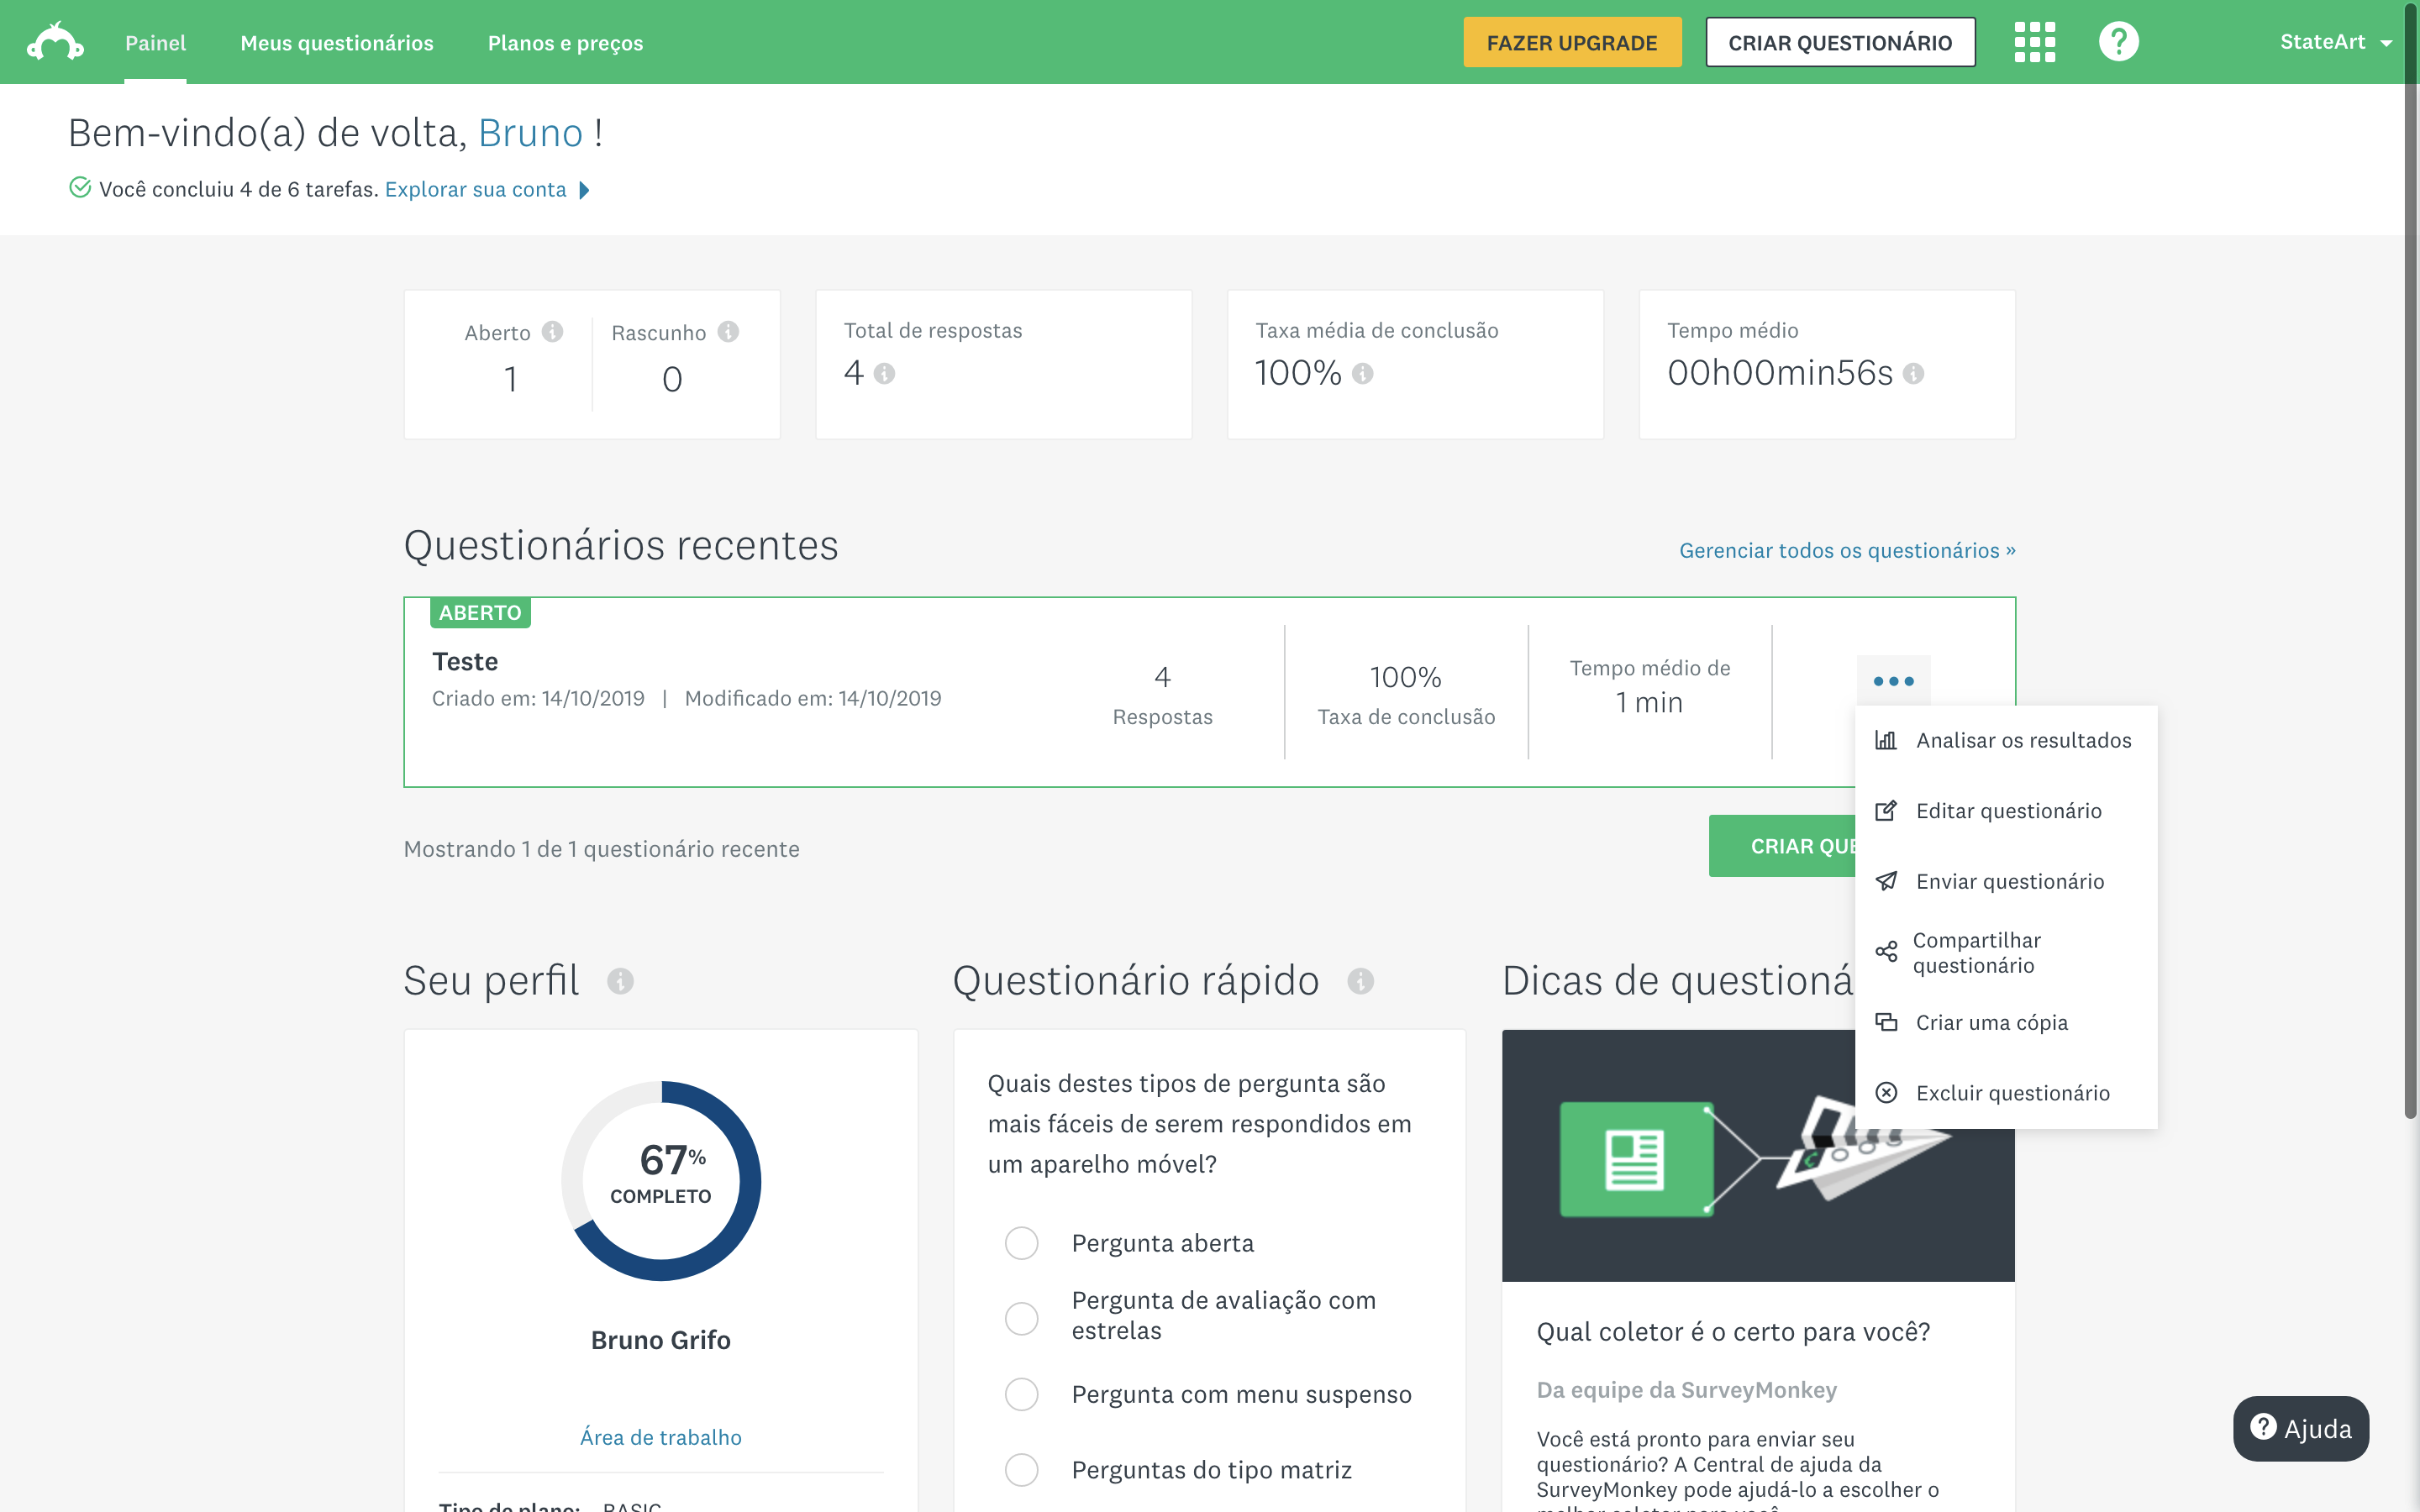
\includegraphics[width=1\textwidth]{img/sm/survey-dashboard}
		\caption{SurveyMonkey - Painel de Controle }
		\label{fig:survey-dashboard}
	\end{center}
\end{figure}

\newpage

\begin{figure}[ht!]
	\begin{center}
		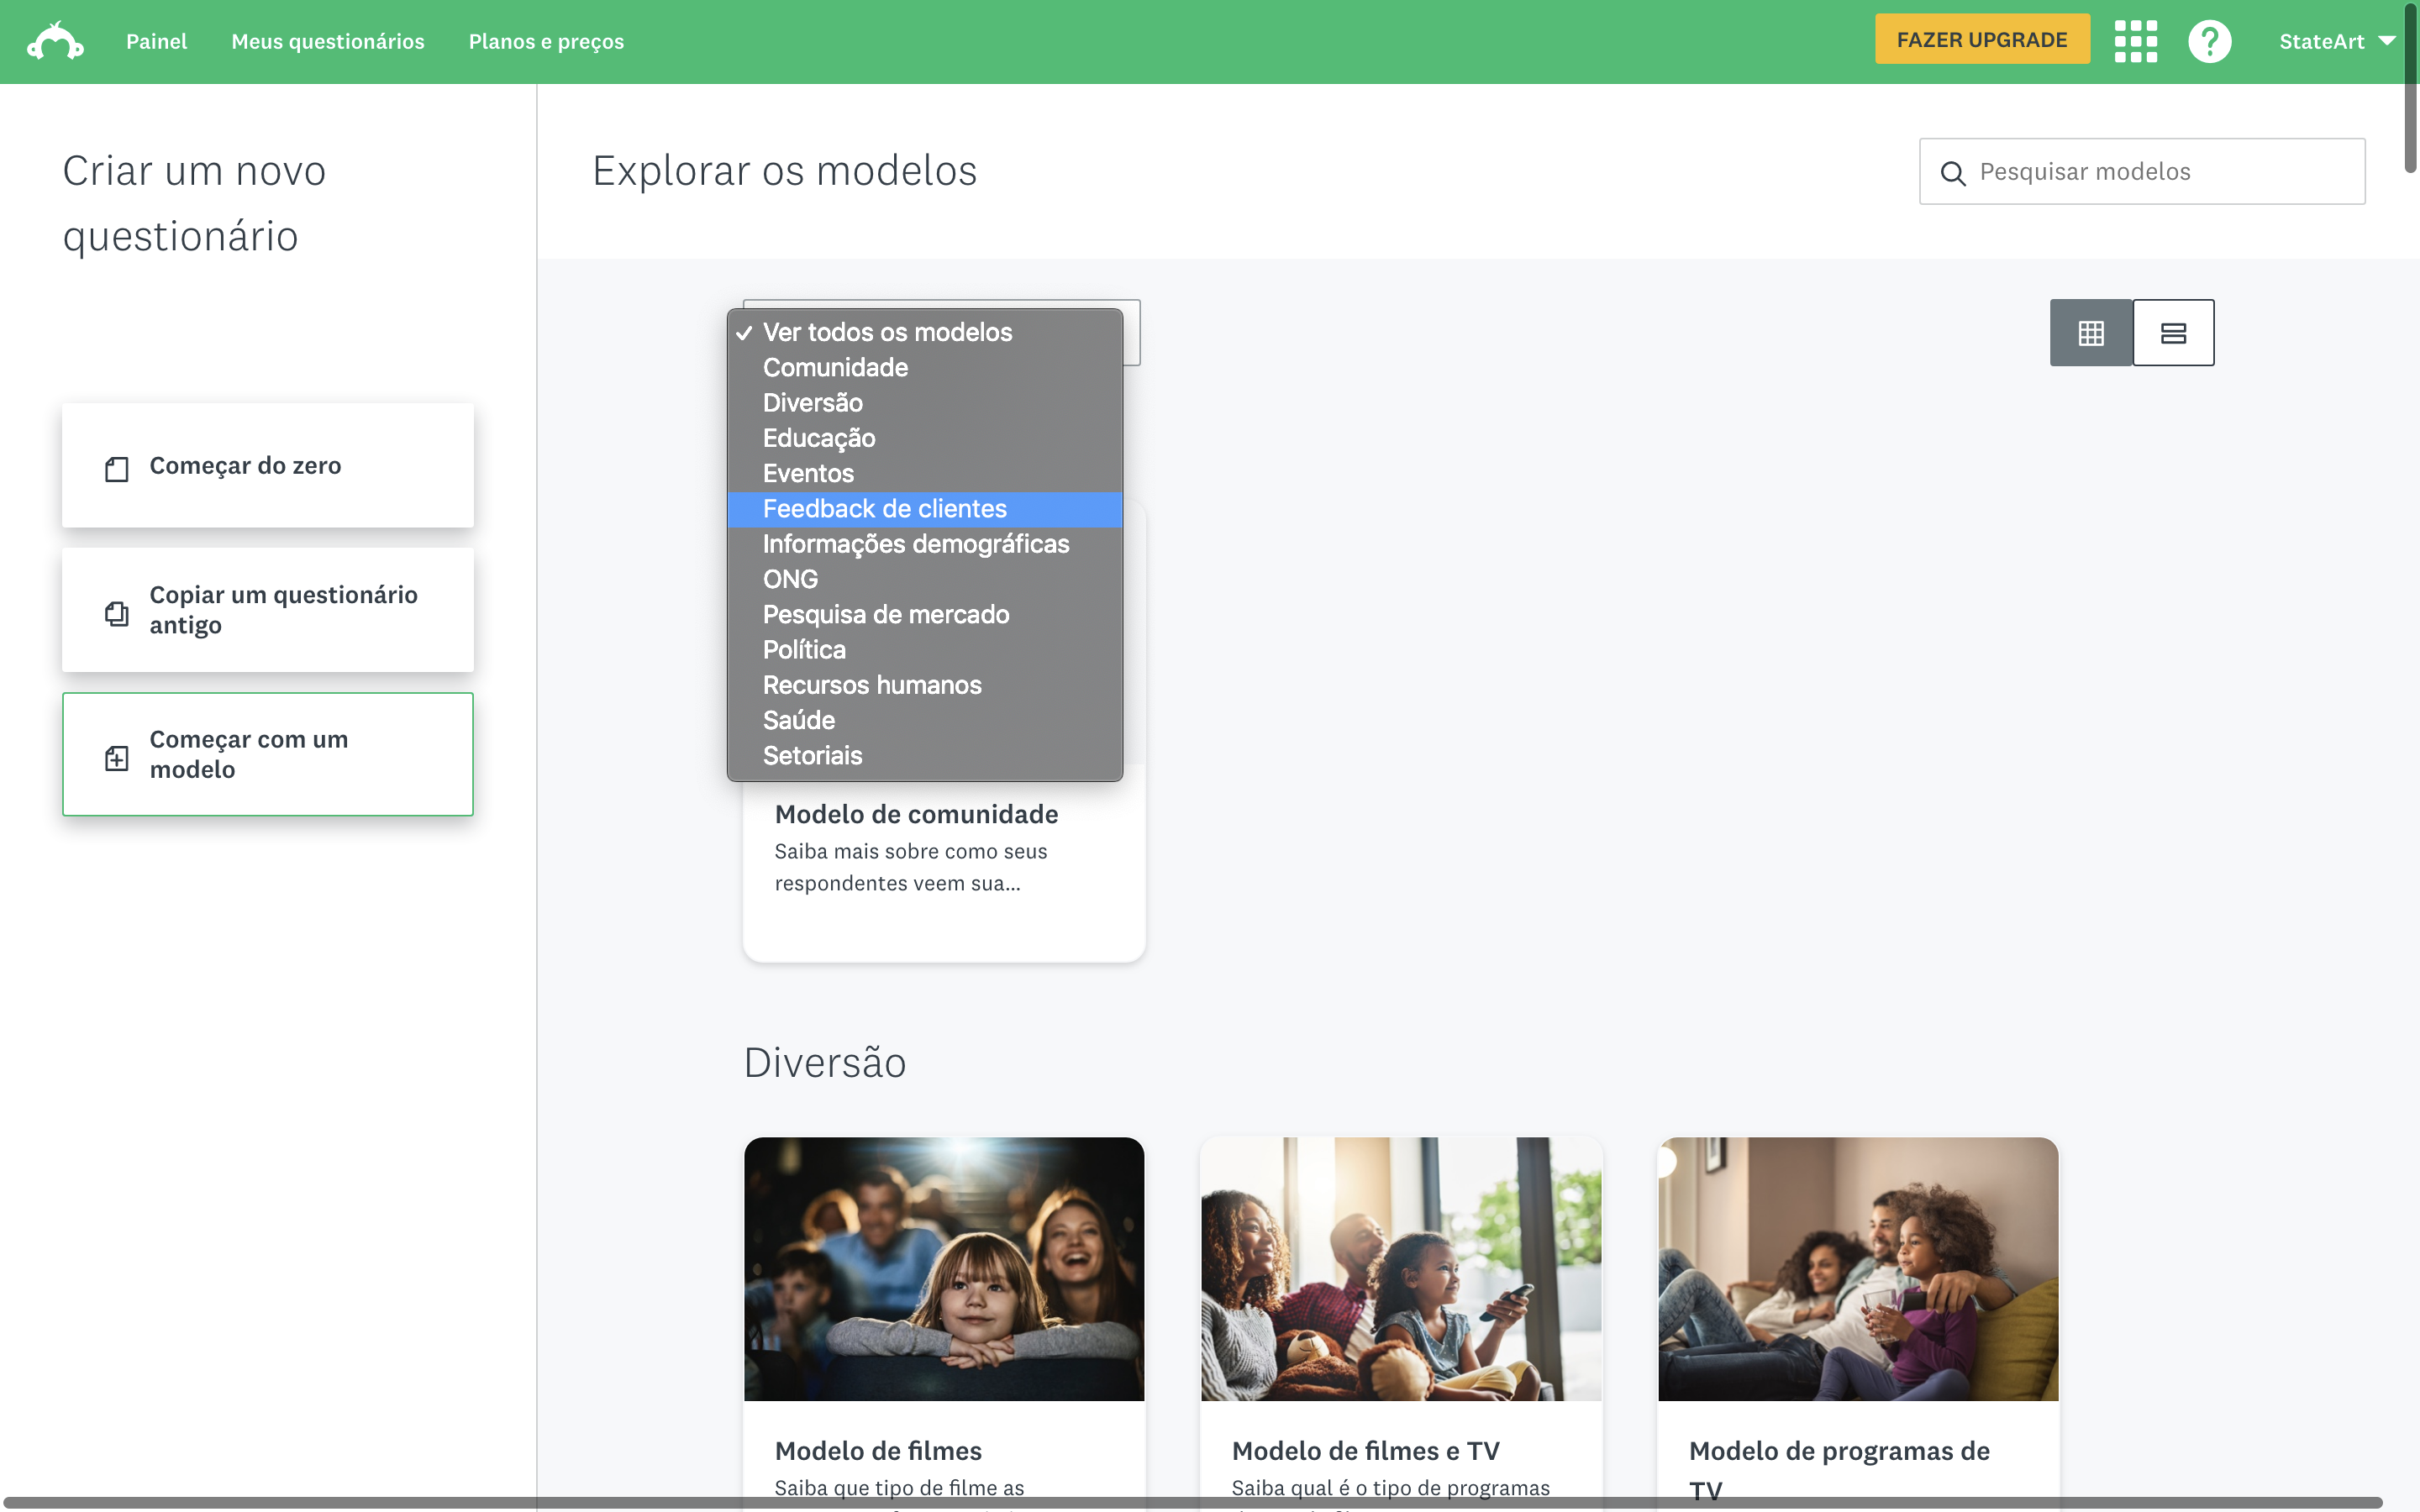
\includegraphics[width=1\textwidth]{img/sm/survey-form-create}
		\caption{SurveyMonkey - Formulários modelo }
		\label{fig:survey-form-create}
	\end{center}
\end{figure}

Quando se inicializa a criação de um novo formulário, a plataforma dá opção de começar do zero ou de utilizar um formulário modelo como podemos ver na Figura \ref{fig:survey-form-create}. Começando um formulário do zero como podemos ver na Figura \ref{fig:survey-form-banck2}, temos acesso a uma série de funcionalidades que vamos explorar e analisar em seguida.

\begin{figure}[ht!]
	\begin{center}
		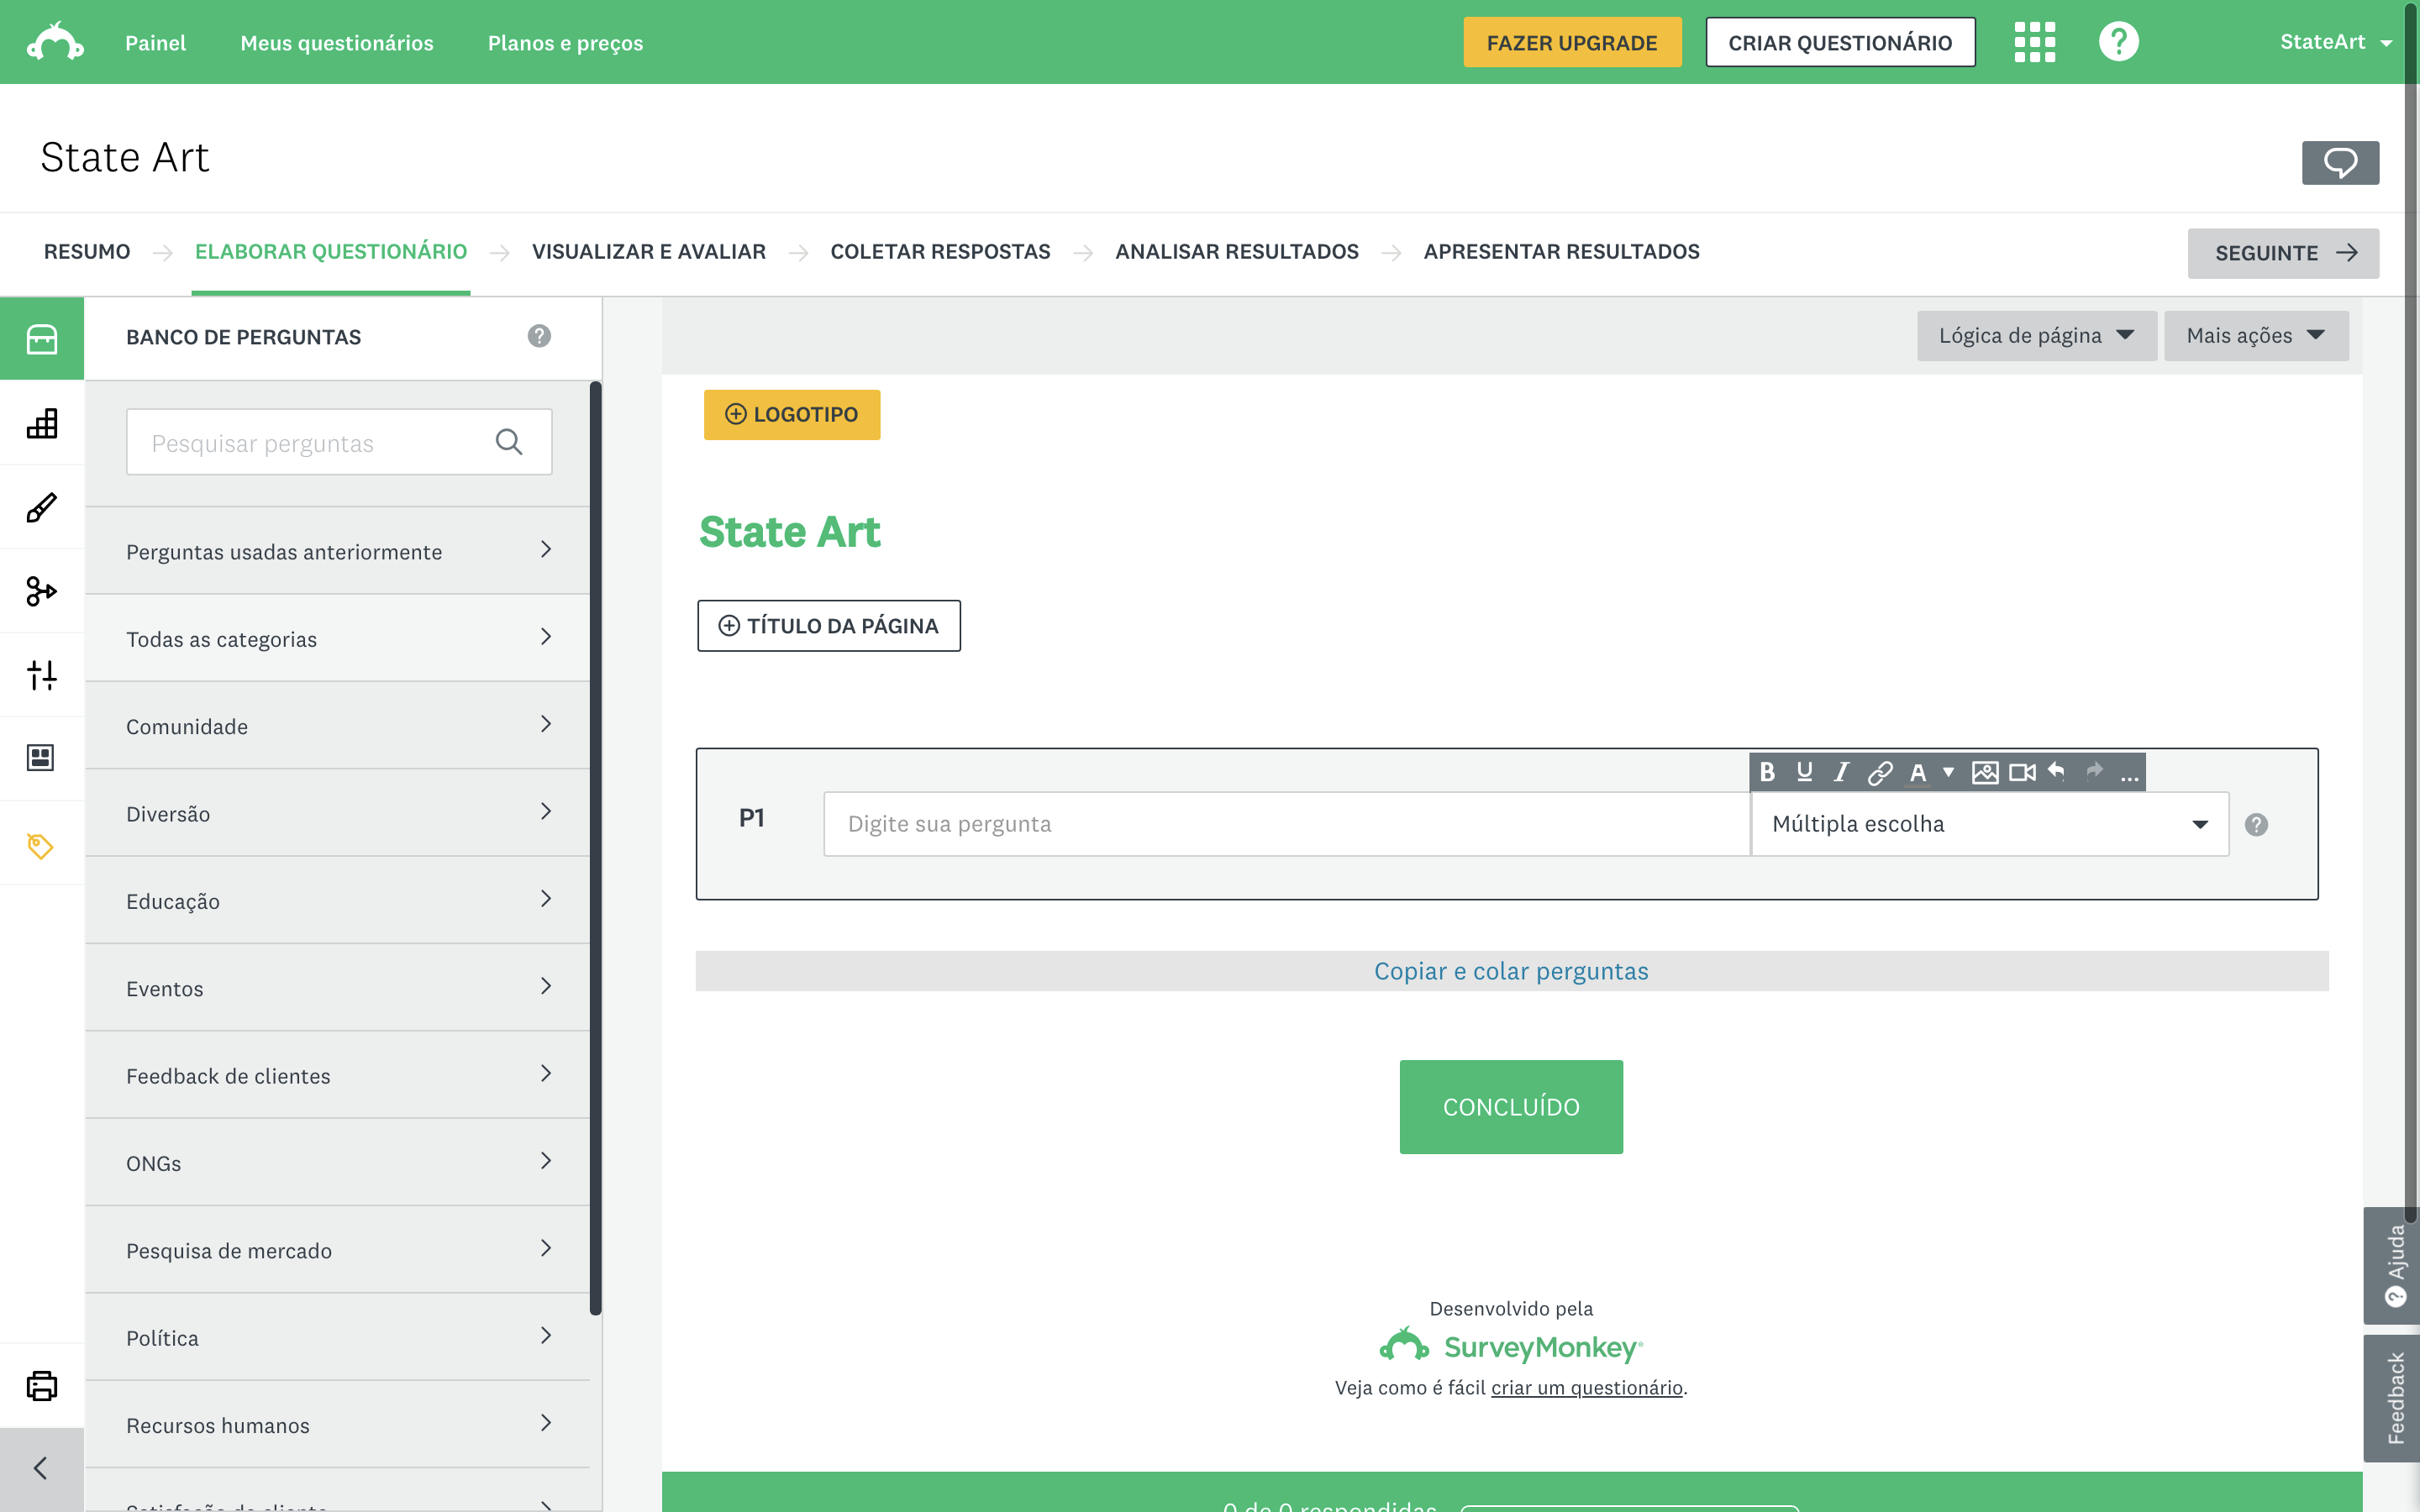
\includegraphics[width=1\textwidth]{img/sm/survey-form-bank2}
		\caption{SurveyMonkey -  Perguntas Modelo}
		\label{fig:survey-form-banck2}
	\end{center}
\end{figure}


\begin{figure}[ht!]
	\begin{center}
		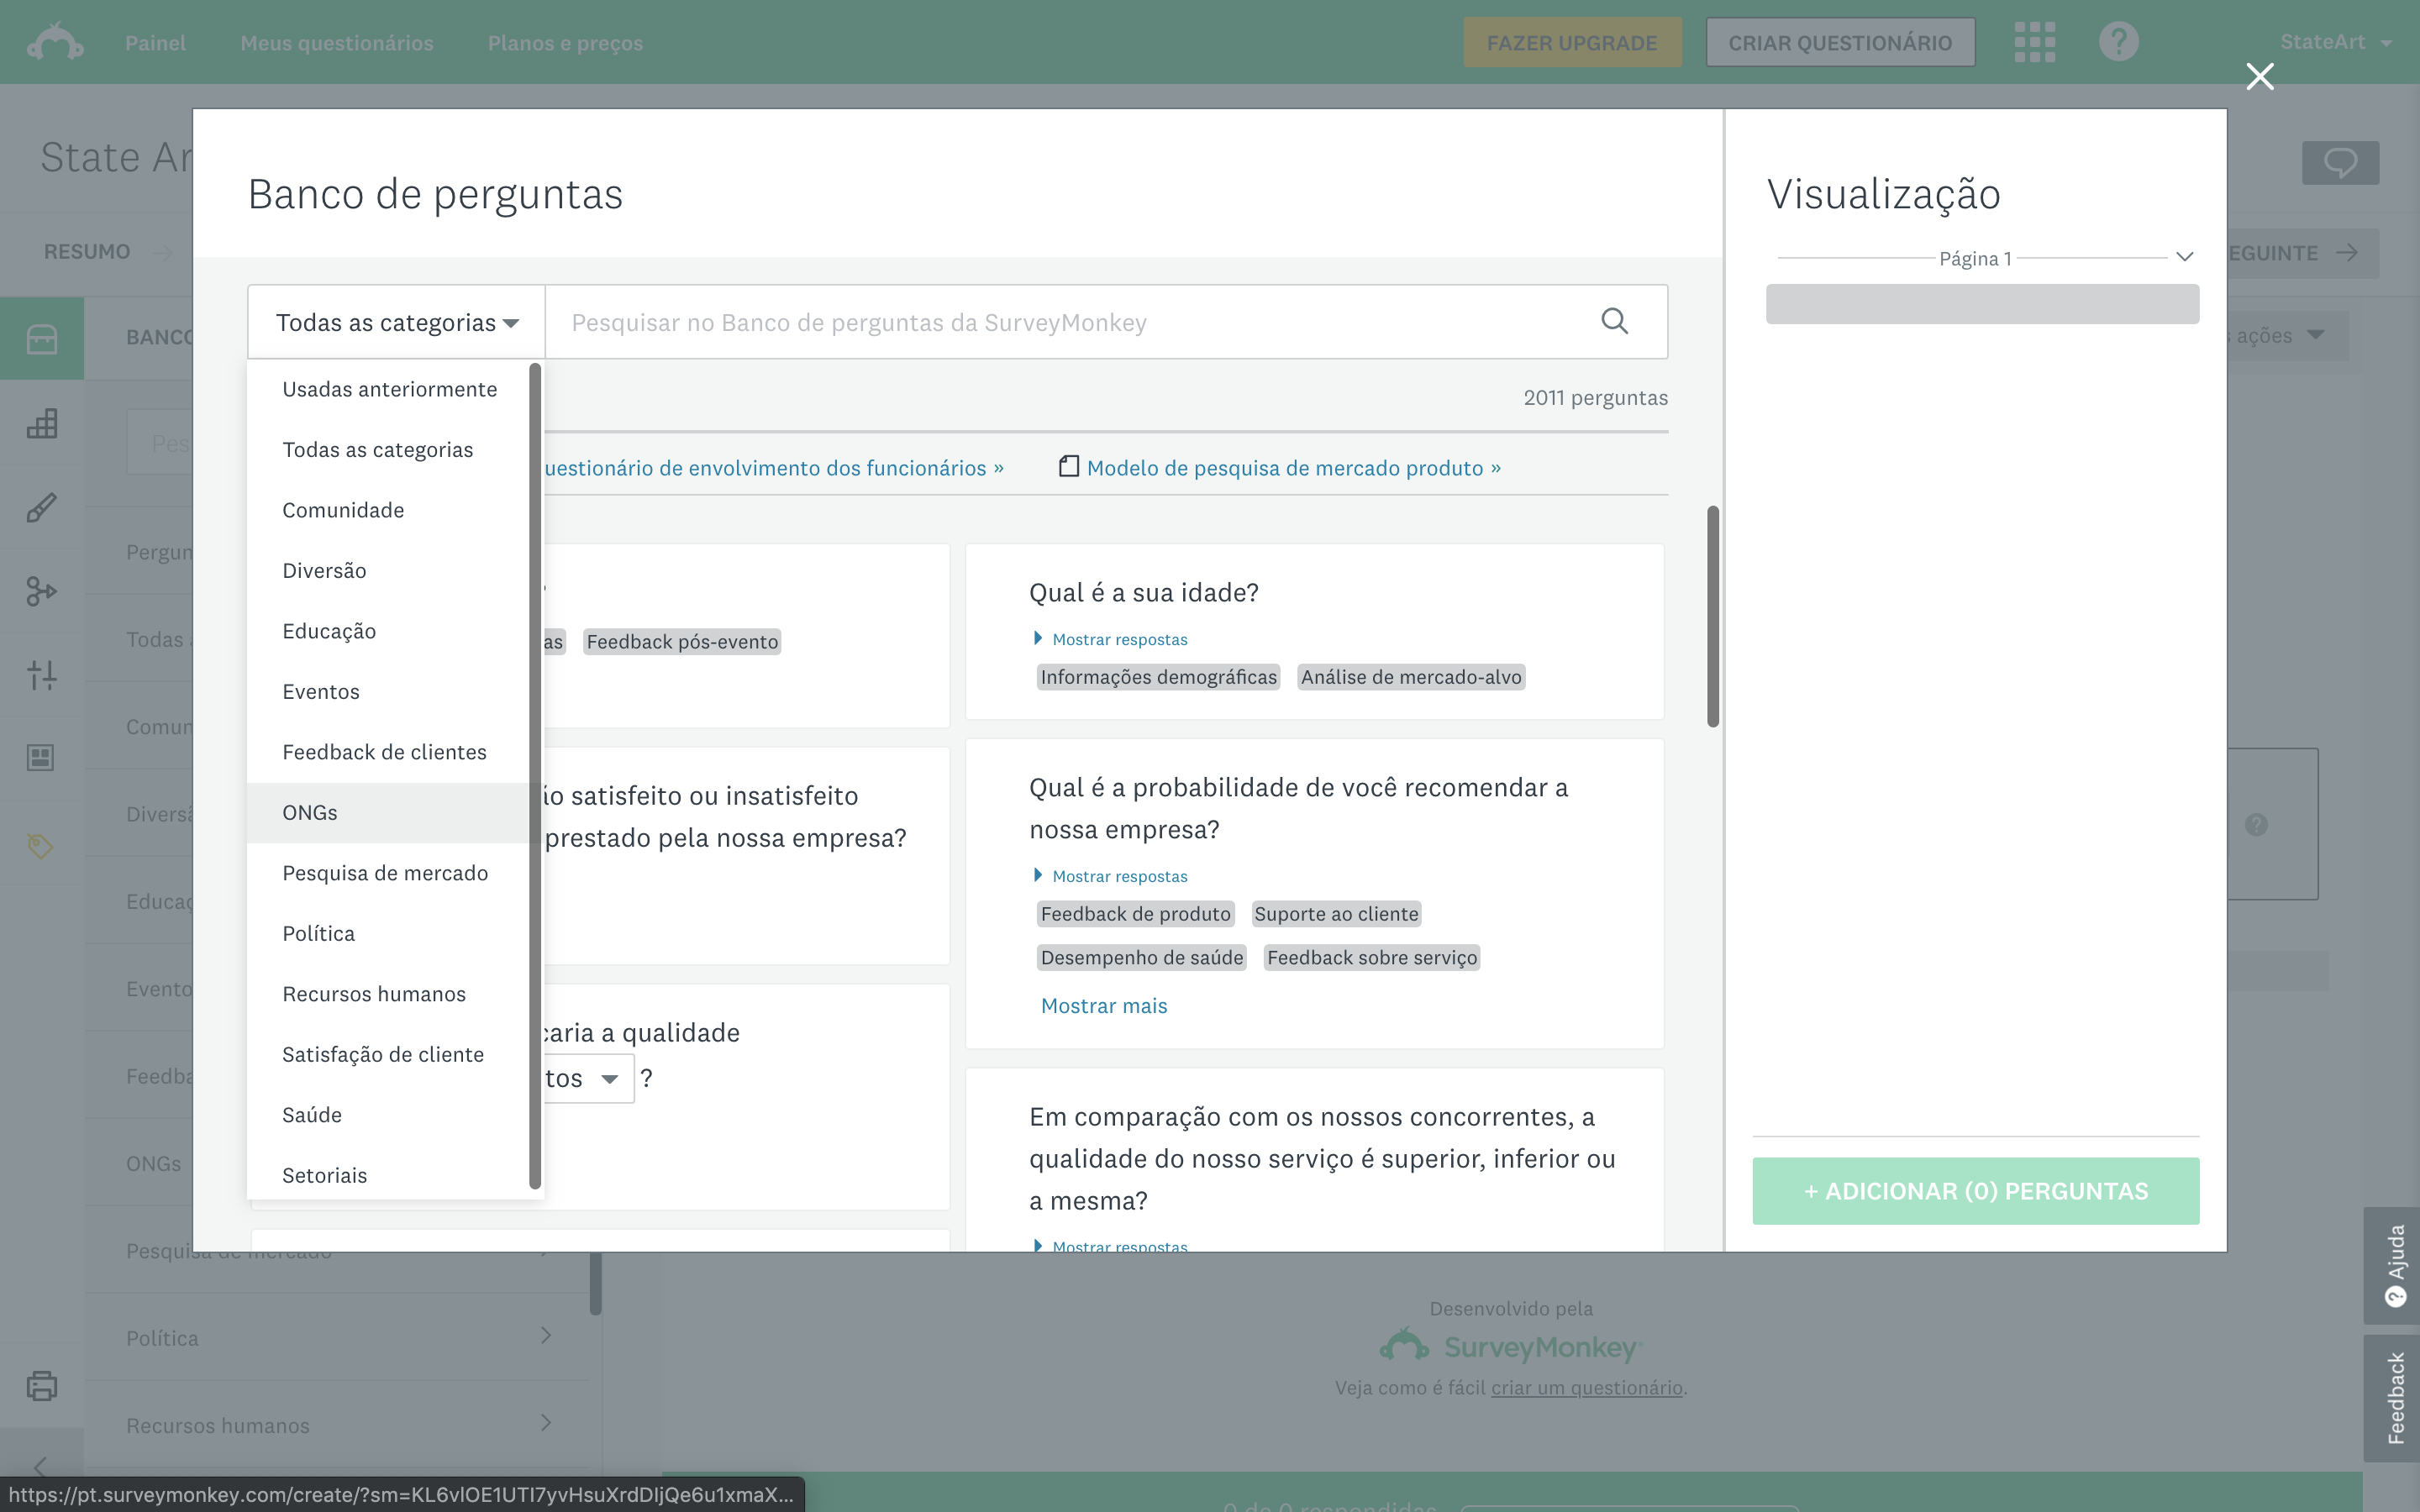
\includegraphics[width=1\textwidth]{img/sm/survey-form-bank1}
		\caption{SurveyMonkey - Perguntas Modelo }
		\label{fig:survey-form-banck1}
	\end{center}
\end{figure}

\newpage

São diversos os elementos que se podem adicionar ou arrastar para o formulário (i. e. perguntas, escolha multipla, imagens...) como representado na Figura \ref{fig:surveymonkey-form-element} e há também um banco de perguntas modelo/recomendações já construídas, organizadas por categorias como podemos ver na Figura \ref{fig:survey-form-banck2} e \ref{fig:survey-form-banck1}.


\begin{figure}[ht!]
	\begin{center}
		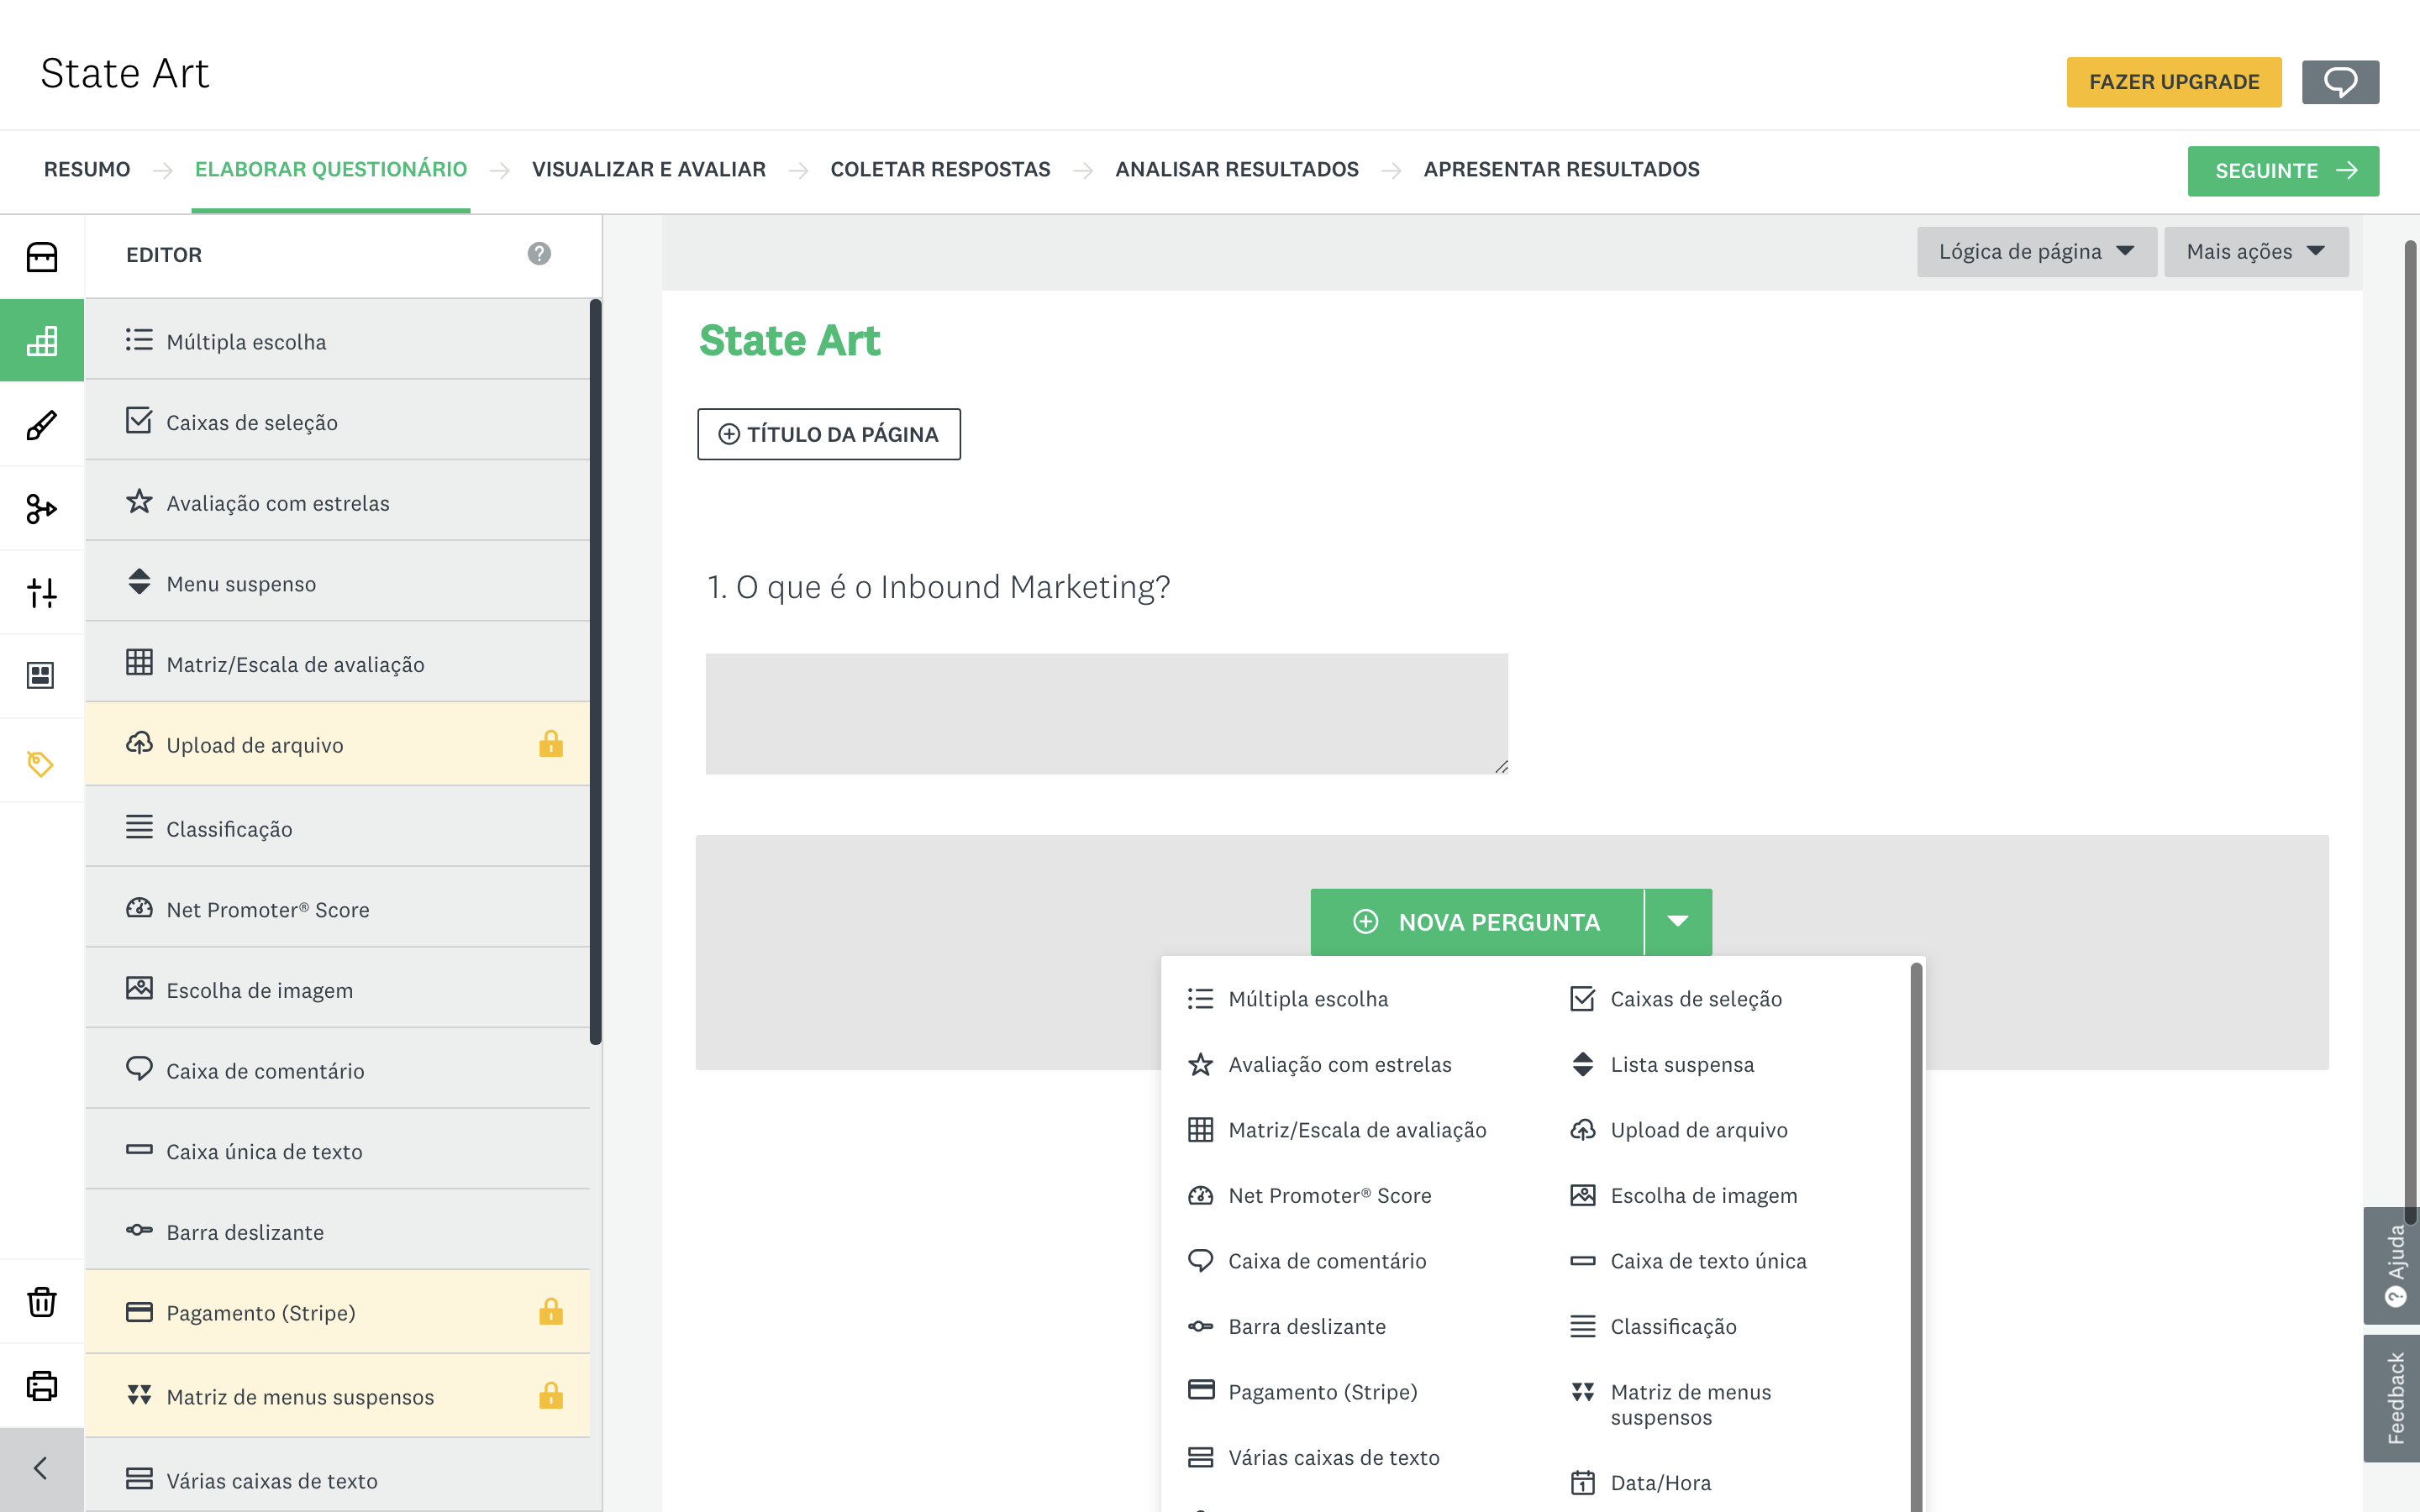
\includegraphics[width=1\textwidth]{img/sm/surveymonkey-form-element}
		\caption{SurveyMonkey - Elementos }
		\label{fig:surveymonkey-form-element}
	\end{center}
\end{figure}
\newpage

\begin{figure}[ht!]
	\begin{center}
		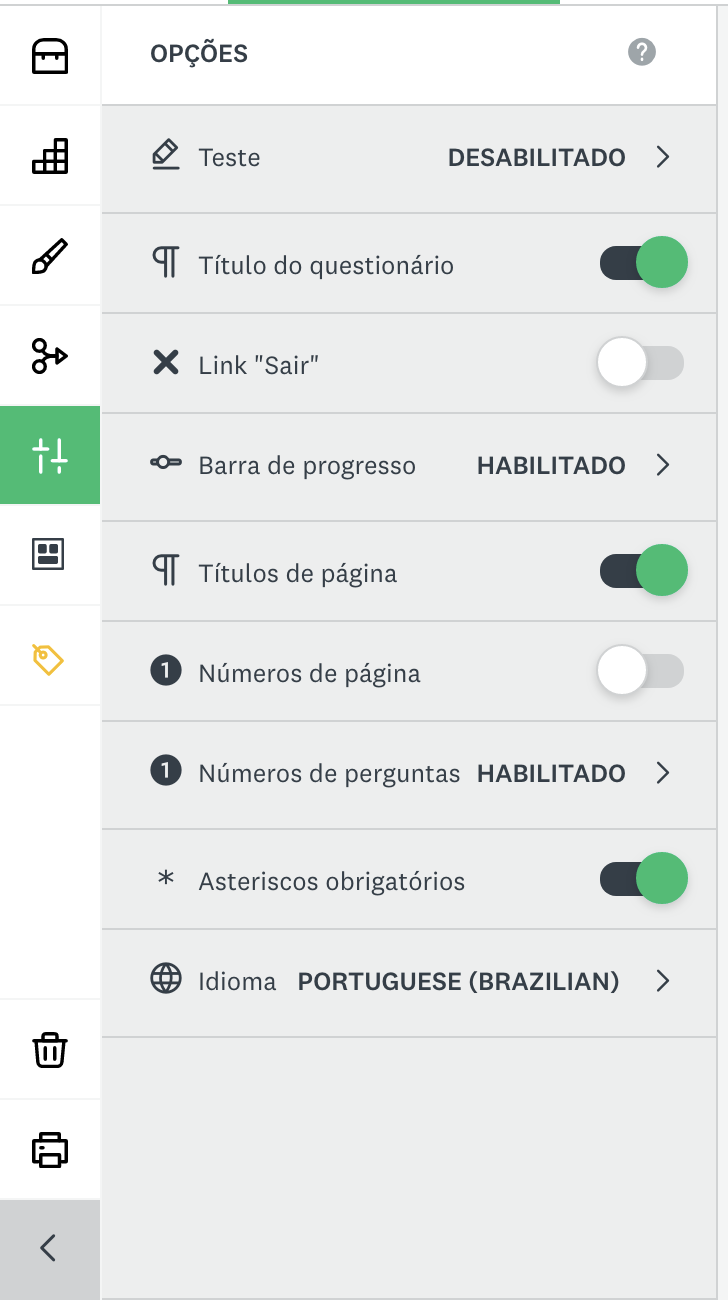
\includegraphics[height=.35\textheight]{img/sm/surveymonkey-form-opcoes}
		\caption{SurveyMonkey - Opções}
		\label{fig:surveymonkey-form-opcoes}
	\end{center}
\end{figure}

\begin{figure}[ht!]
	\begin{center}
		\begin{minipage}{0.45\textwidth}
			\begin{center}
				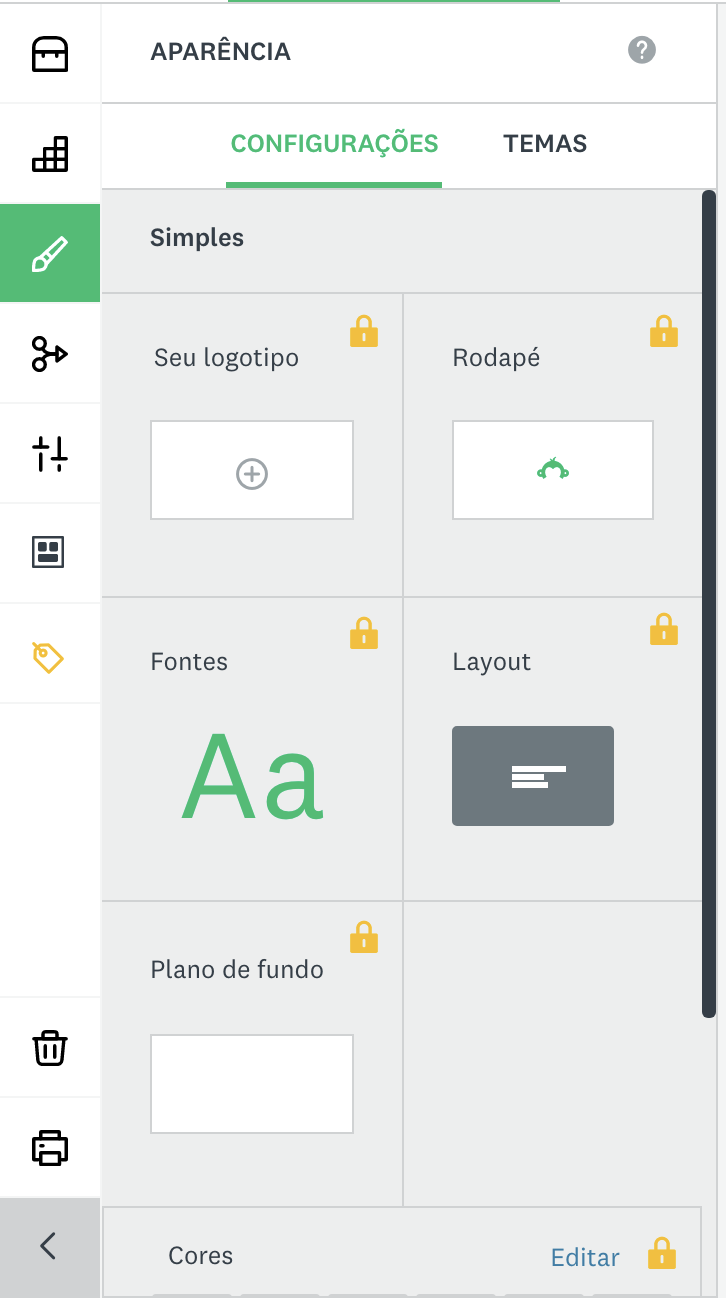
\includegraphics[height=.35\textheight]{img/sm/surveymonkey-form-aparencia}
				\caption{SurveyMonkey - Aparência}
				\label{fig:surveymonkey-form-aparencia}
			\end{center}
		\end{minipage}
		\hspace{1cm}
		\begin{minipage}{0.45\textwidth}
			\begin{center}
				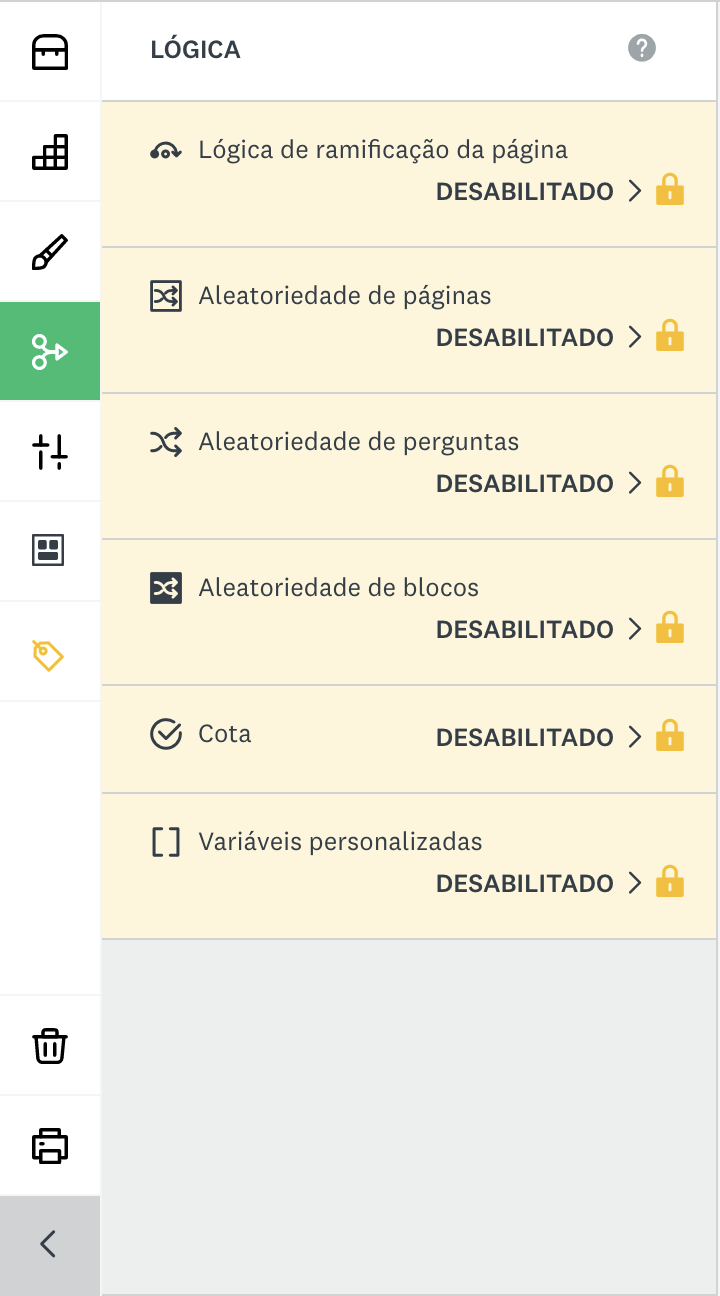
\includegraphics[height=.35\textheight]{img/sm/surveymonkey-form-logica}
				\caption{SurveyMonkey - Lógica}
				\label{fig:surveymonkey-form-logica}
			\end{center}
		\end{minipage}
	\end{center}
\end{figure}

O SurveyMonkey permite também realizar algumas operações de personalização do formulário. Nas Figuras \ref{fig:surveymonkey-form-opcoes}, \ref{fig:surveymonkey-form-aparencia} e \ref{fig:surveymonkey-form-logica} estão representaçãs as opções, aparência e lógica do formulário, respetivamente, que permite costumizar formulários ao público alvo. 
Depois de realizado o formulário esta plataforma permite a visualização do mesmo, em diferentes tipos de dispositivos, como se pode ver nas Figuras \ref{fig:surveymonkey-form-test-pc} e \ref{fig:surveymonkey-form-test-phone}, para verificar se tudo está conforme planeado para se poder prosseguir para a recolha de dados. 
\newpage

\begin{figure}[ht!]
	\begin{center}
		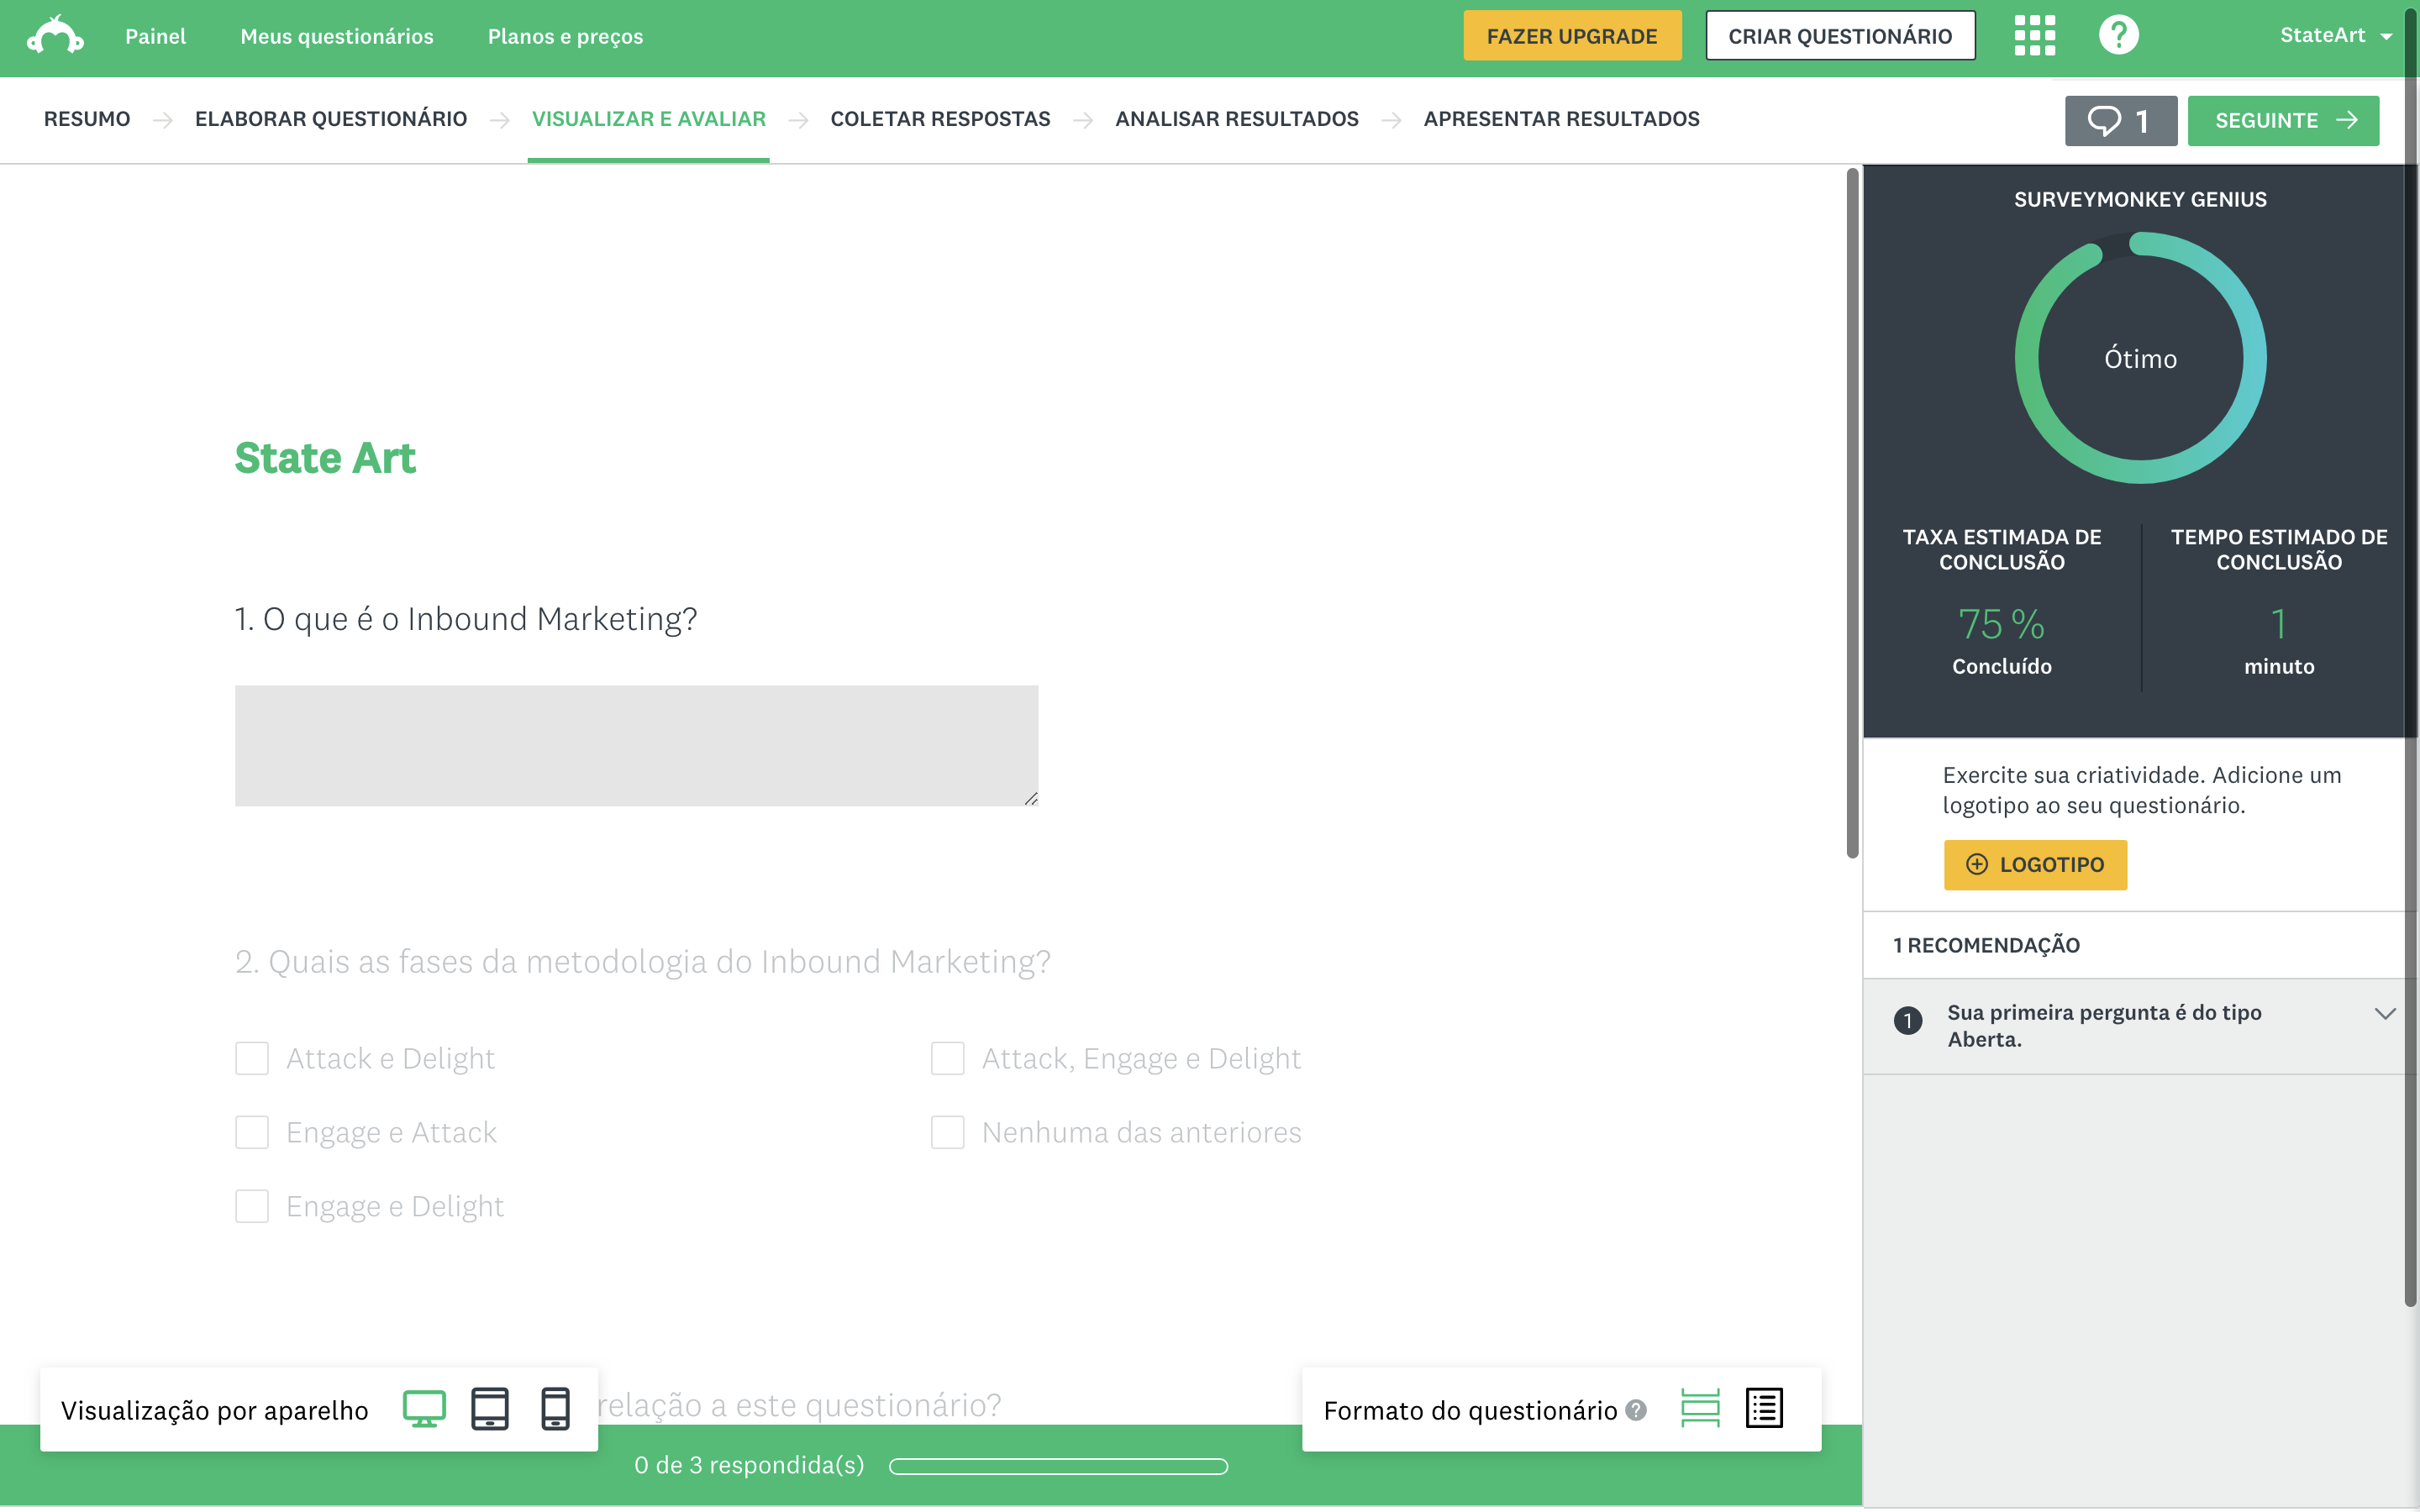
\includegraphics[width=1\textwidth]{img/sm/surveymonkey-form-test-pc}
		\caption{SurveyMonkey - Visualização do formulário em computador }
		\label{fig:surveymonkey-form-test-pc}
	\end{center}
\end{figure}

\begin{figure}[ht!]
	\begin{center}
		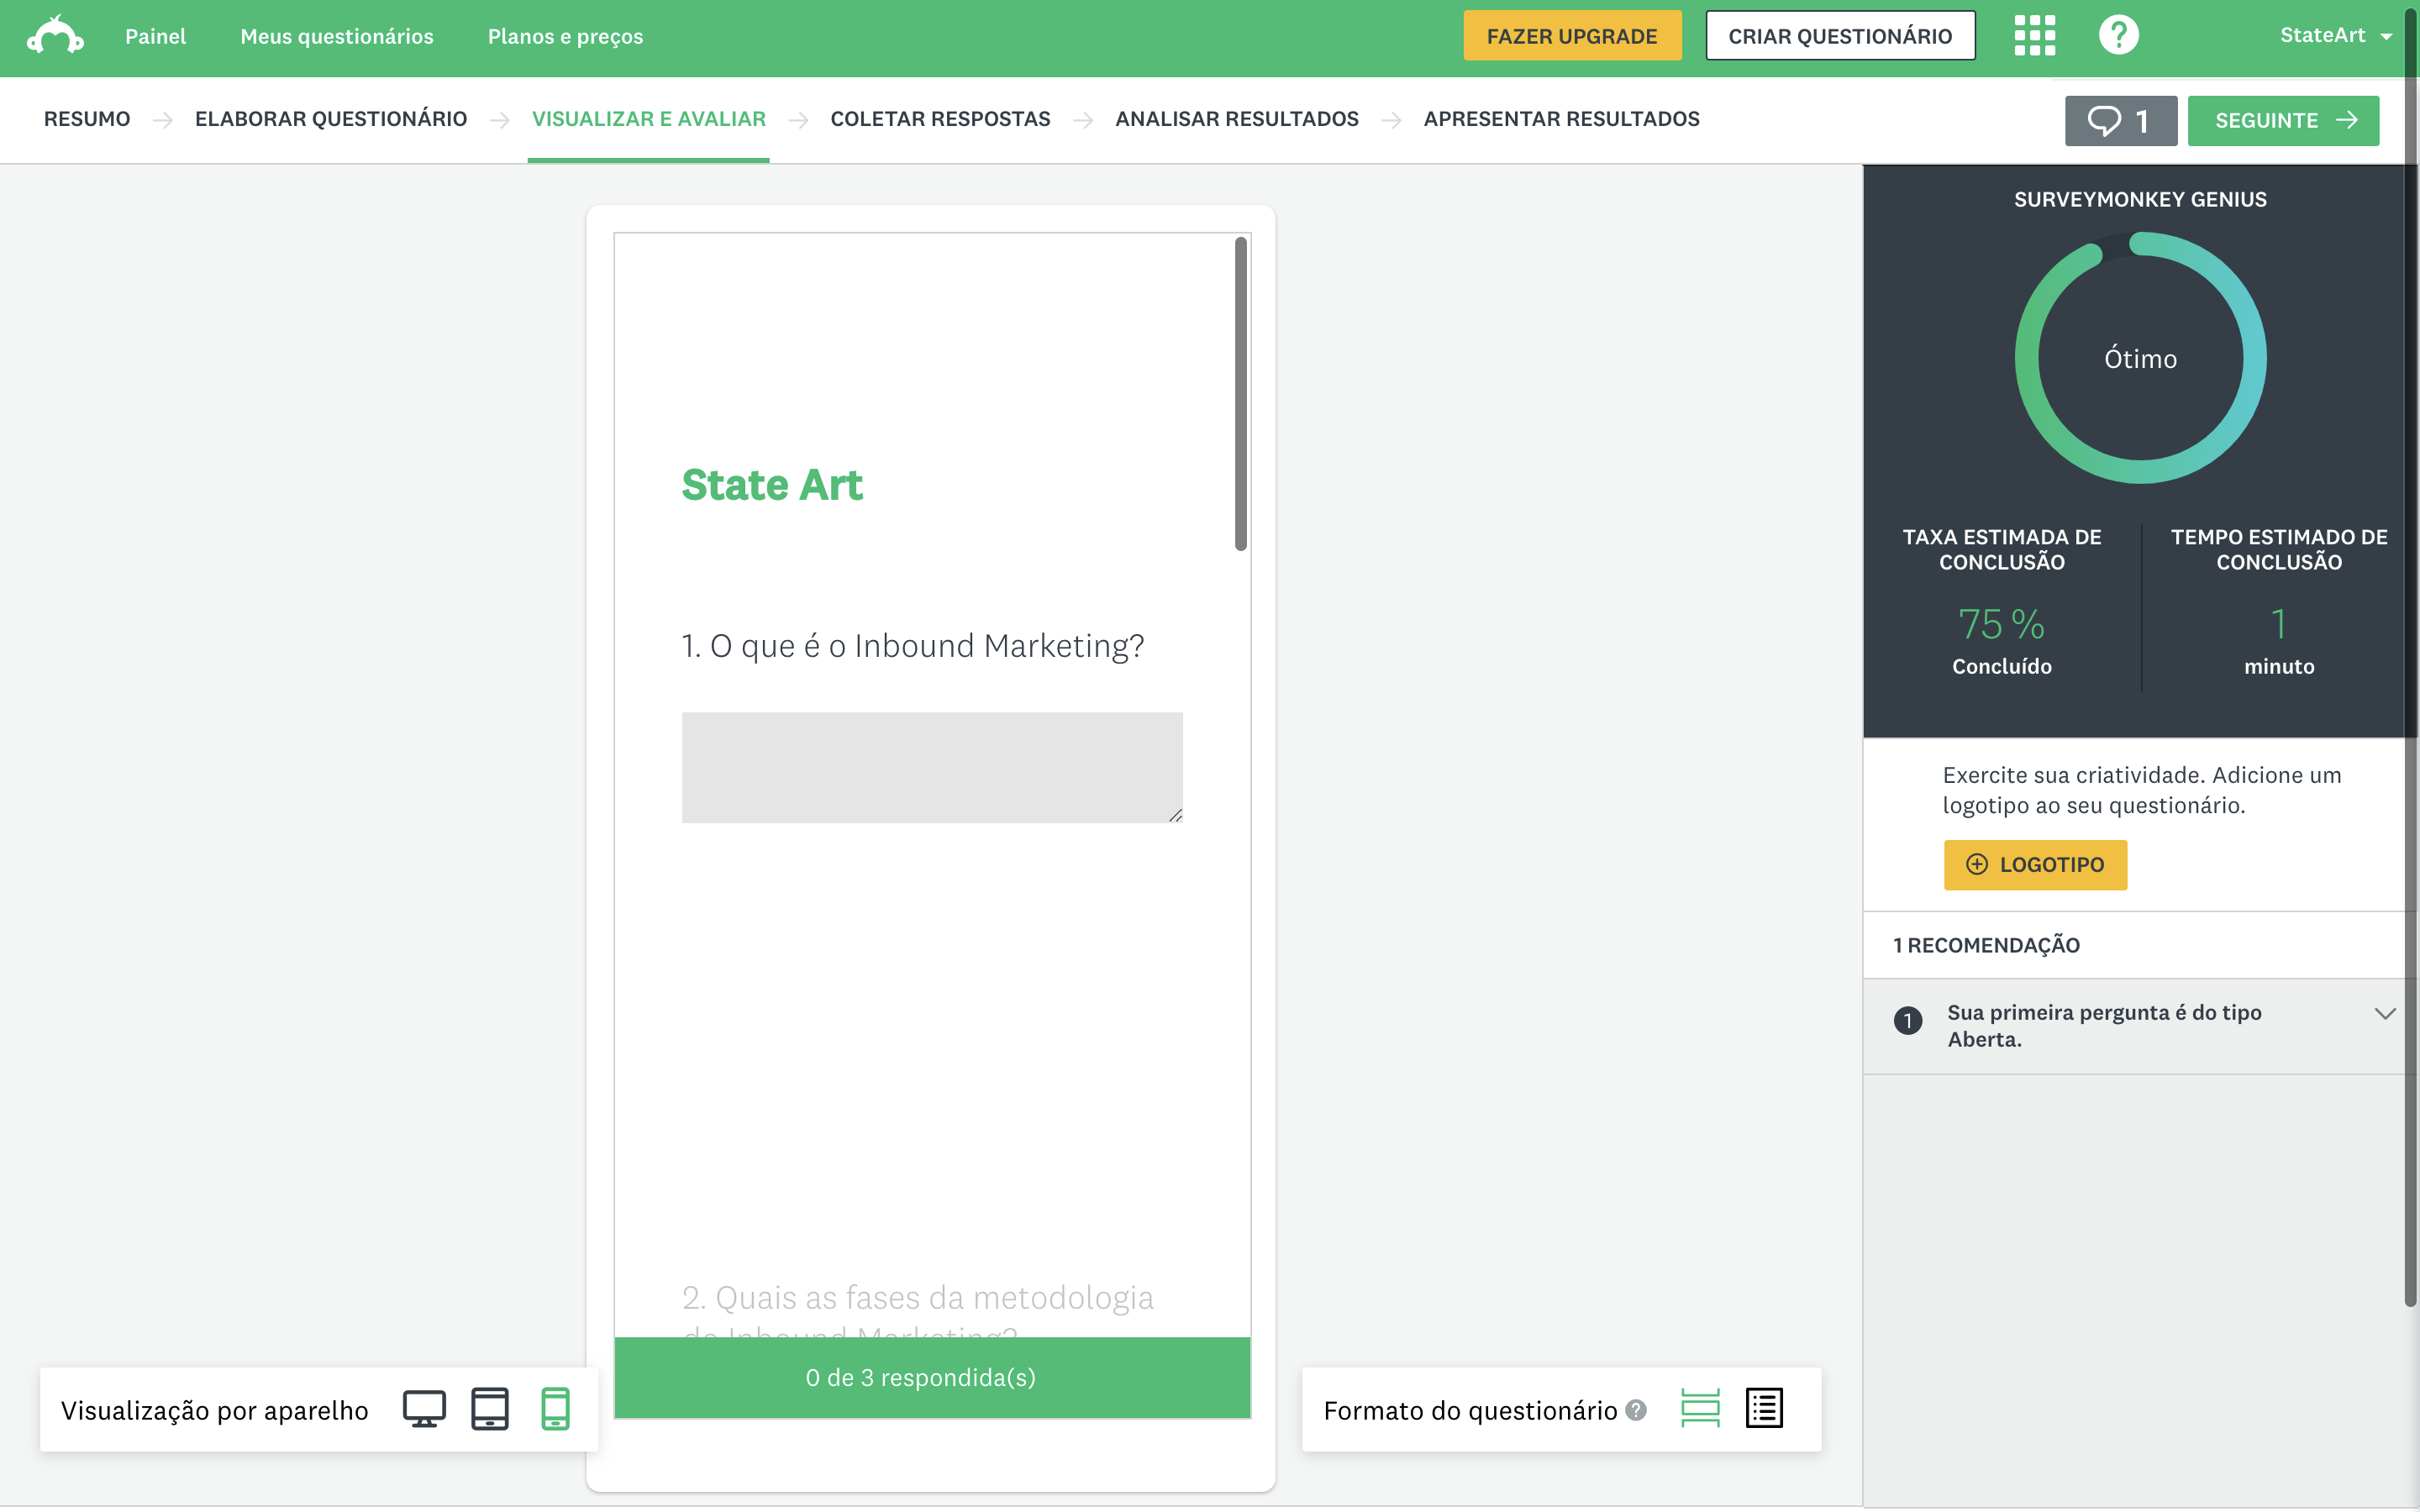
\includegraphics[width=1\textwidth]{img/sm/surveymonkey-form-test-phone}
		\caption{SurveyMonkey - Visualisação do formulário em smartphone }
		\label{fig:surveymonkey-form-test-phone}
	\end{center}
\end{figure}

Depois de garantir que o formulário foi construido como desejado a plataforma fornece vários meios pelo qual se pode partilhar/enviar o formulário, como listado na Figura \ref{fig:surveymonkey-form-share}.

\newpage

\begin{figure}[ht!]
	\begin{center}
		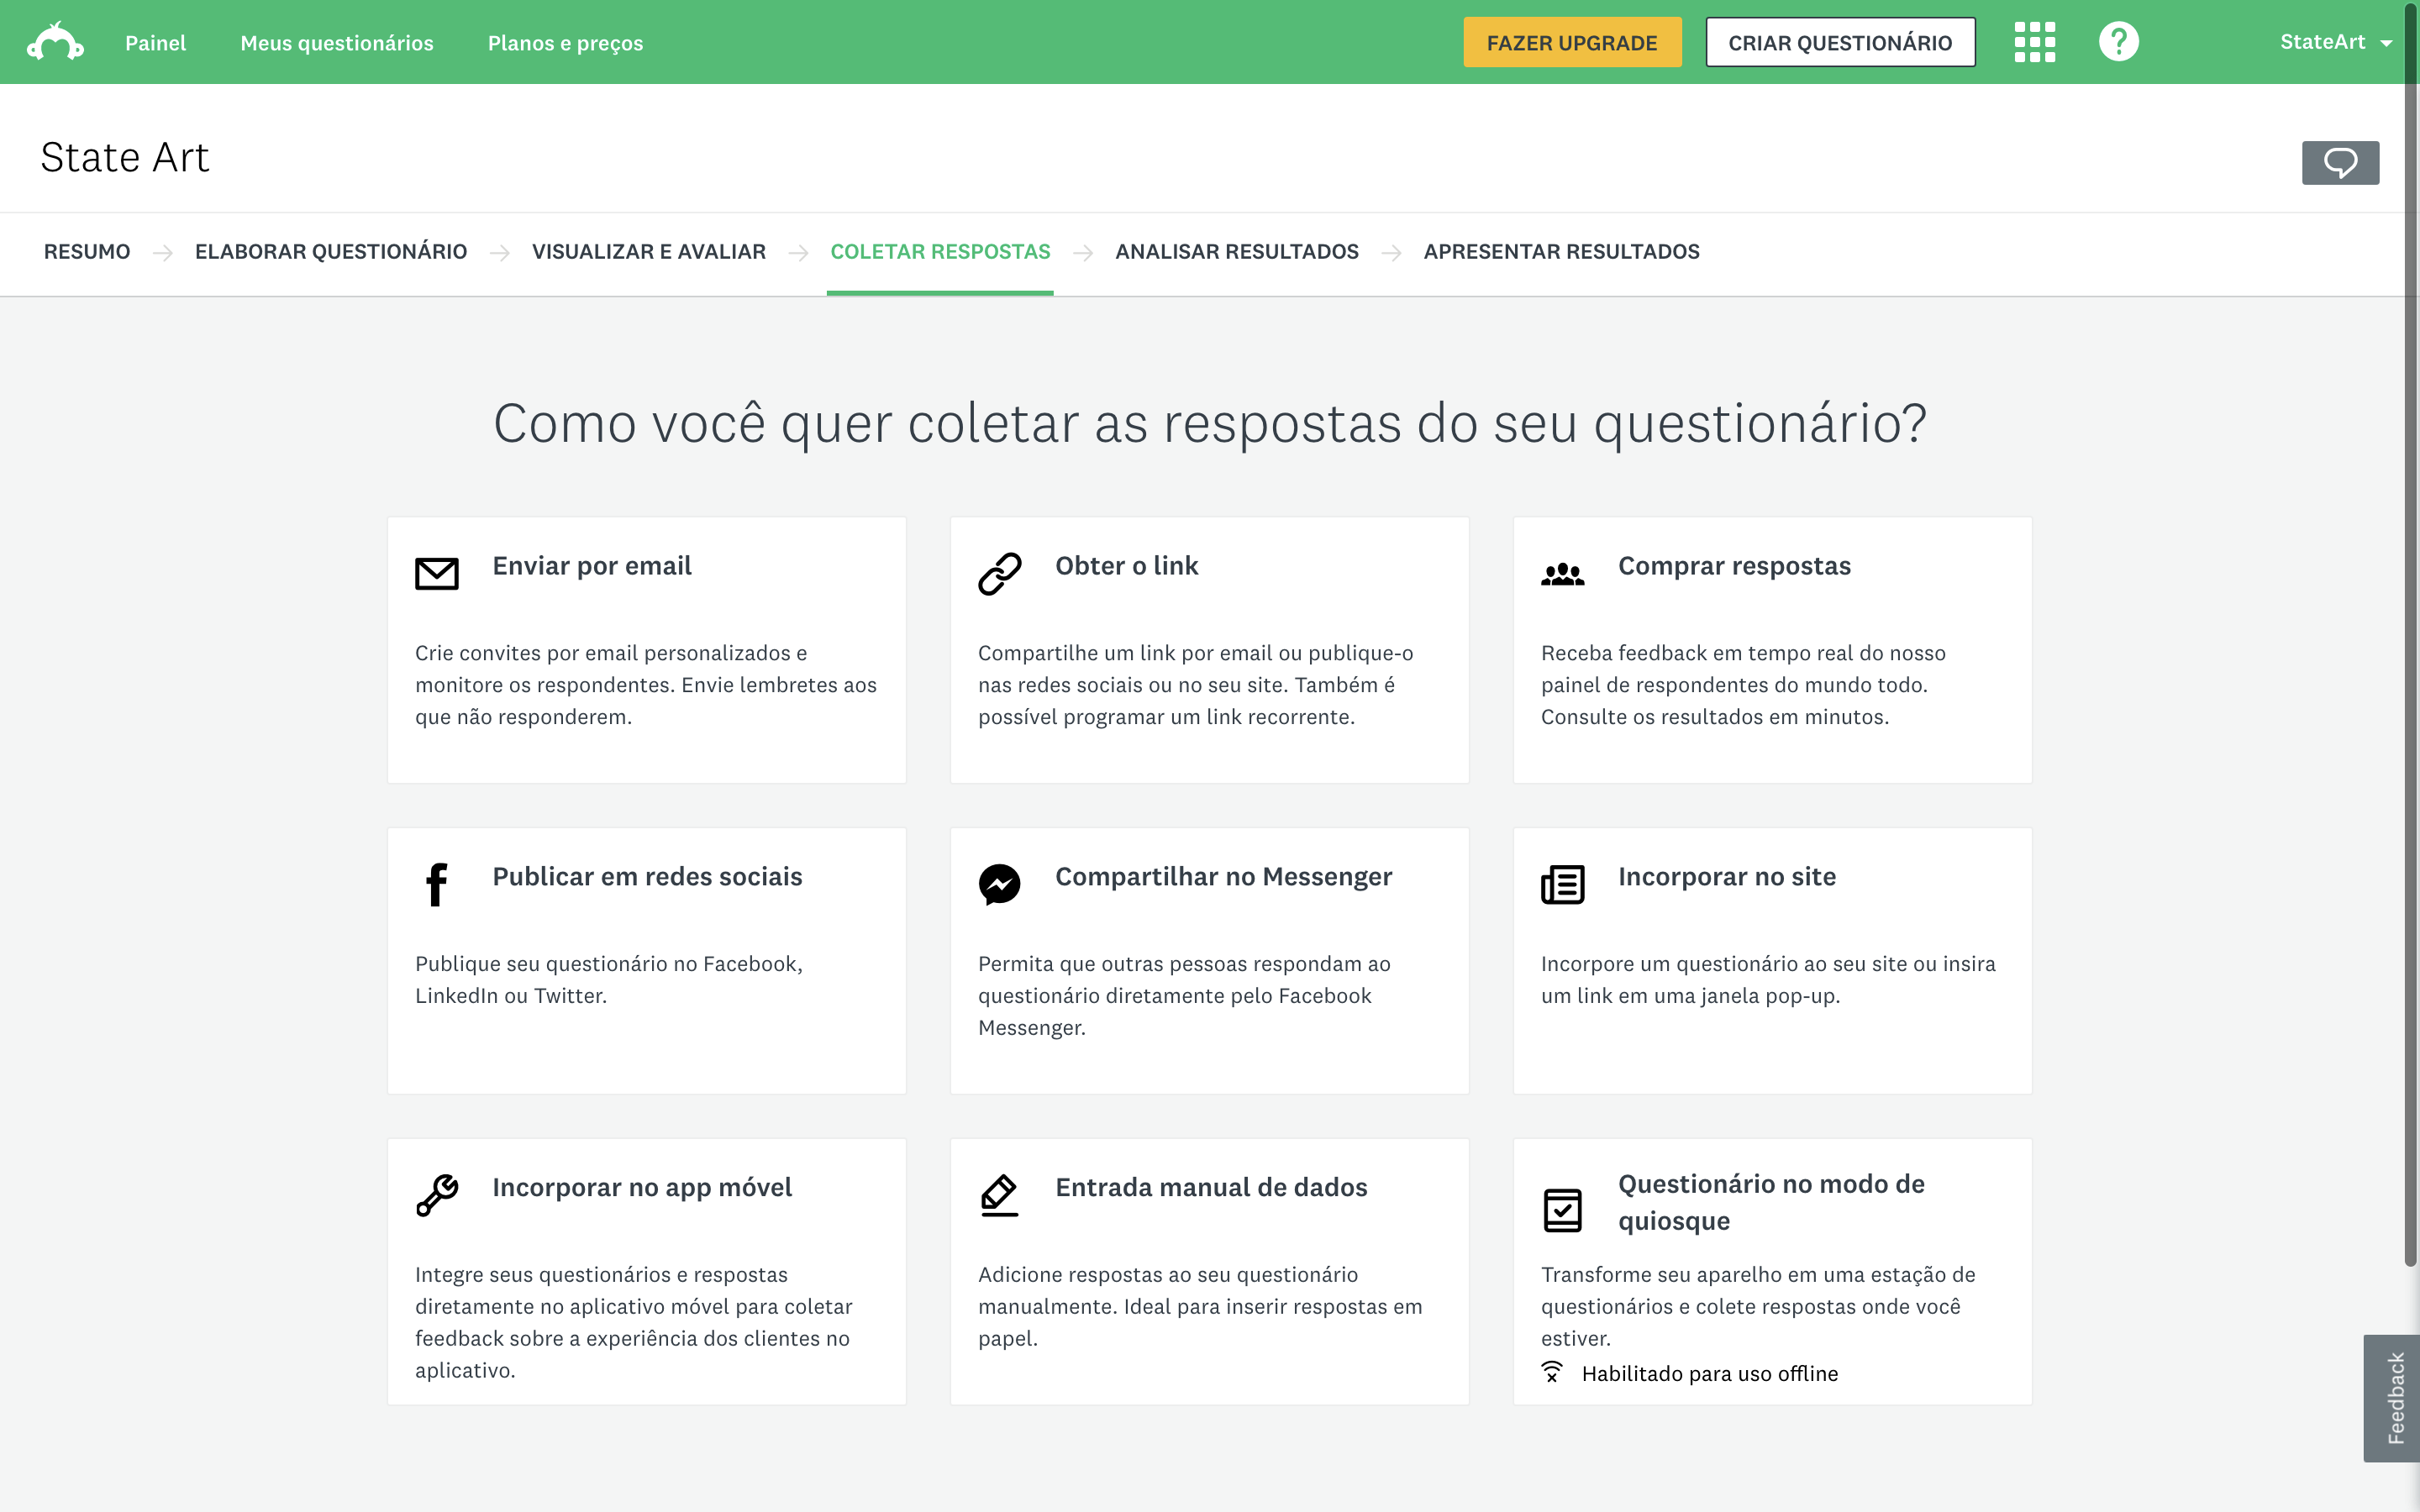
\includegraphics[width=1\textwidth]{img/sm/surveymonkey-form-share}
		\caption{SurveyMonkey - Metodo de partilha do formulário }
		\label{fig:surveymonkey-form-share}
	\end{center}
\end{figure}

Na analise de resultados, é necessário actualizar a página ou aplicar um filtro para que os gráficos e as estatísticas sejam actualizadas. 
O mesmo se passa na página que pode ser gerada para partilhar o sumário dos dados recolhidos, através do formulário. 
Para aplicar um filtro é necessário escolher o tipo de filtro e os elementos ao qual queremos aplicar o filtro como podemos ver nas Figuras \ref{fig:surveymonkey-form-filtro} e \ref{fig:surveymonkey-form-filtro1}. 


\begin{figure}[ht!]
	\begin{center}
		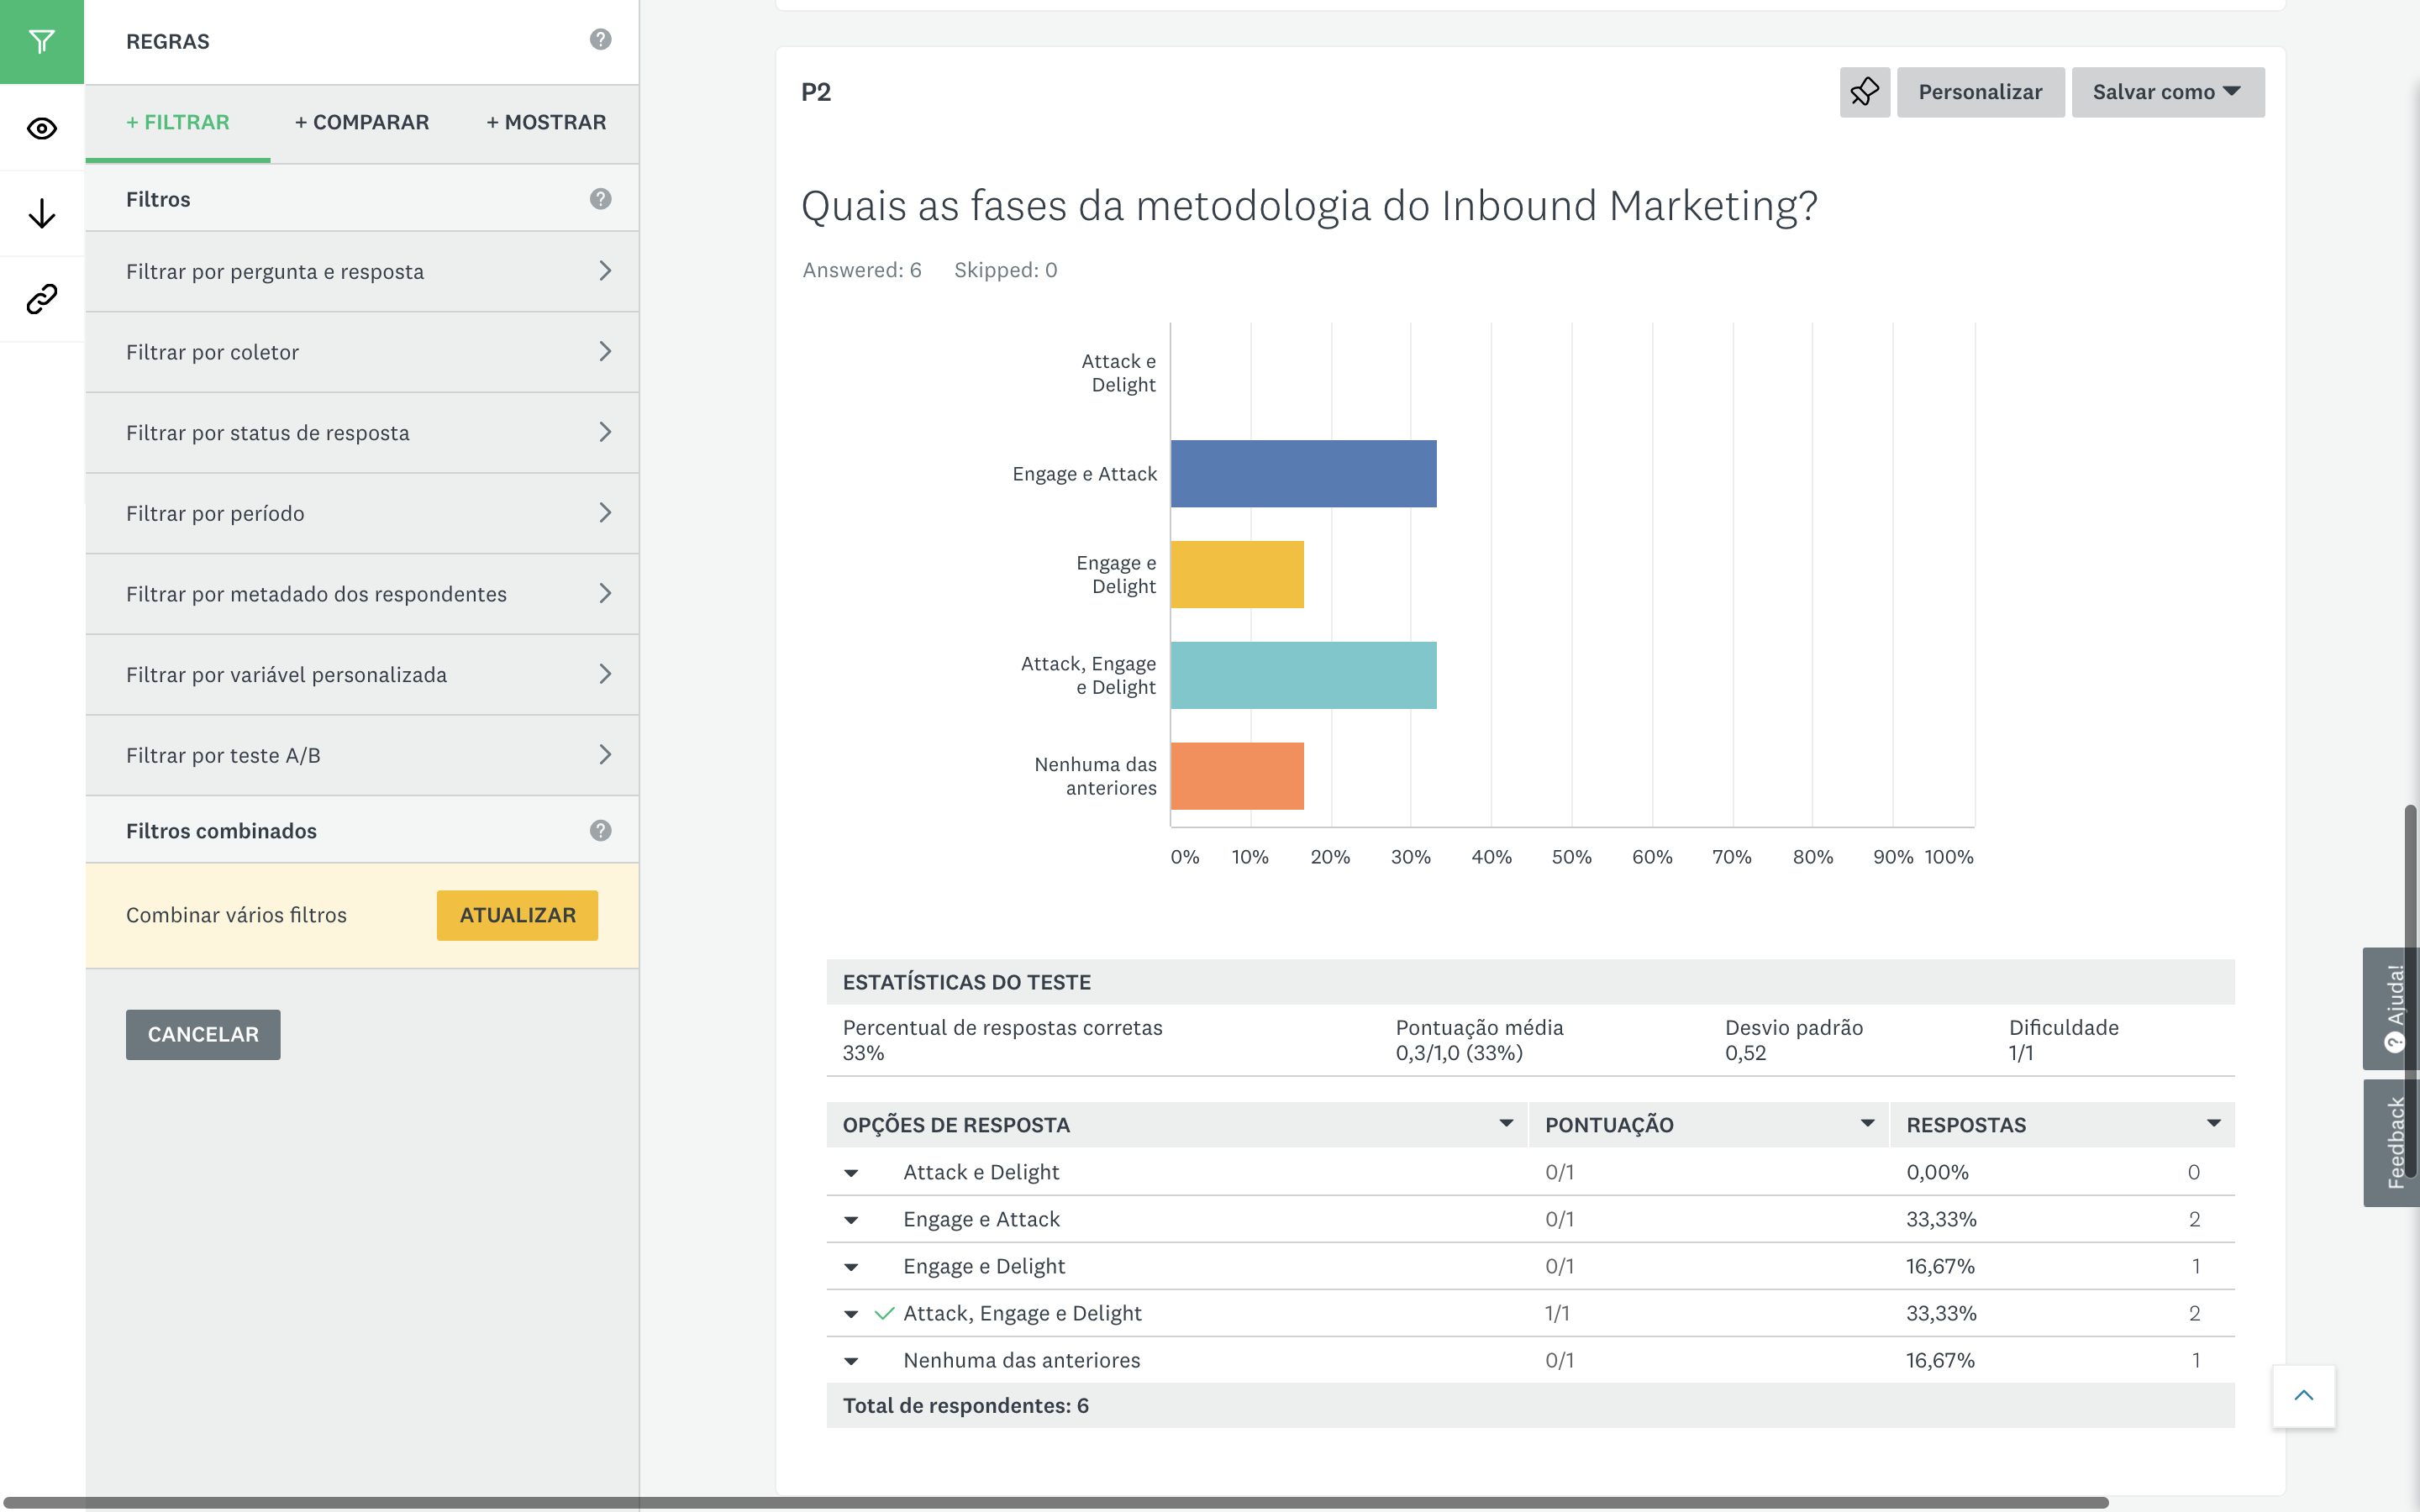
\includegraphics[width=1\textwidth]{img/sm/surveymonkey-form-filtro}
		\caption{SurveyMonkey - Tipos de Filtros }
		\label{fig:surveymonkey-form-filtro}
	\end{center}
\end{figure}



\begin{figure}[ht!]
	\begin{center}
		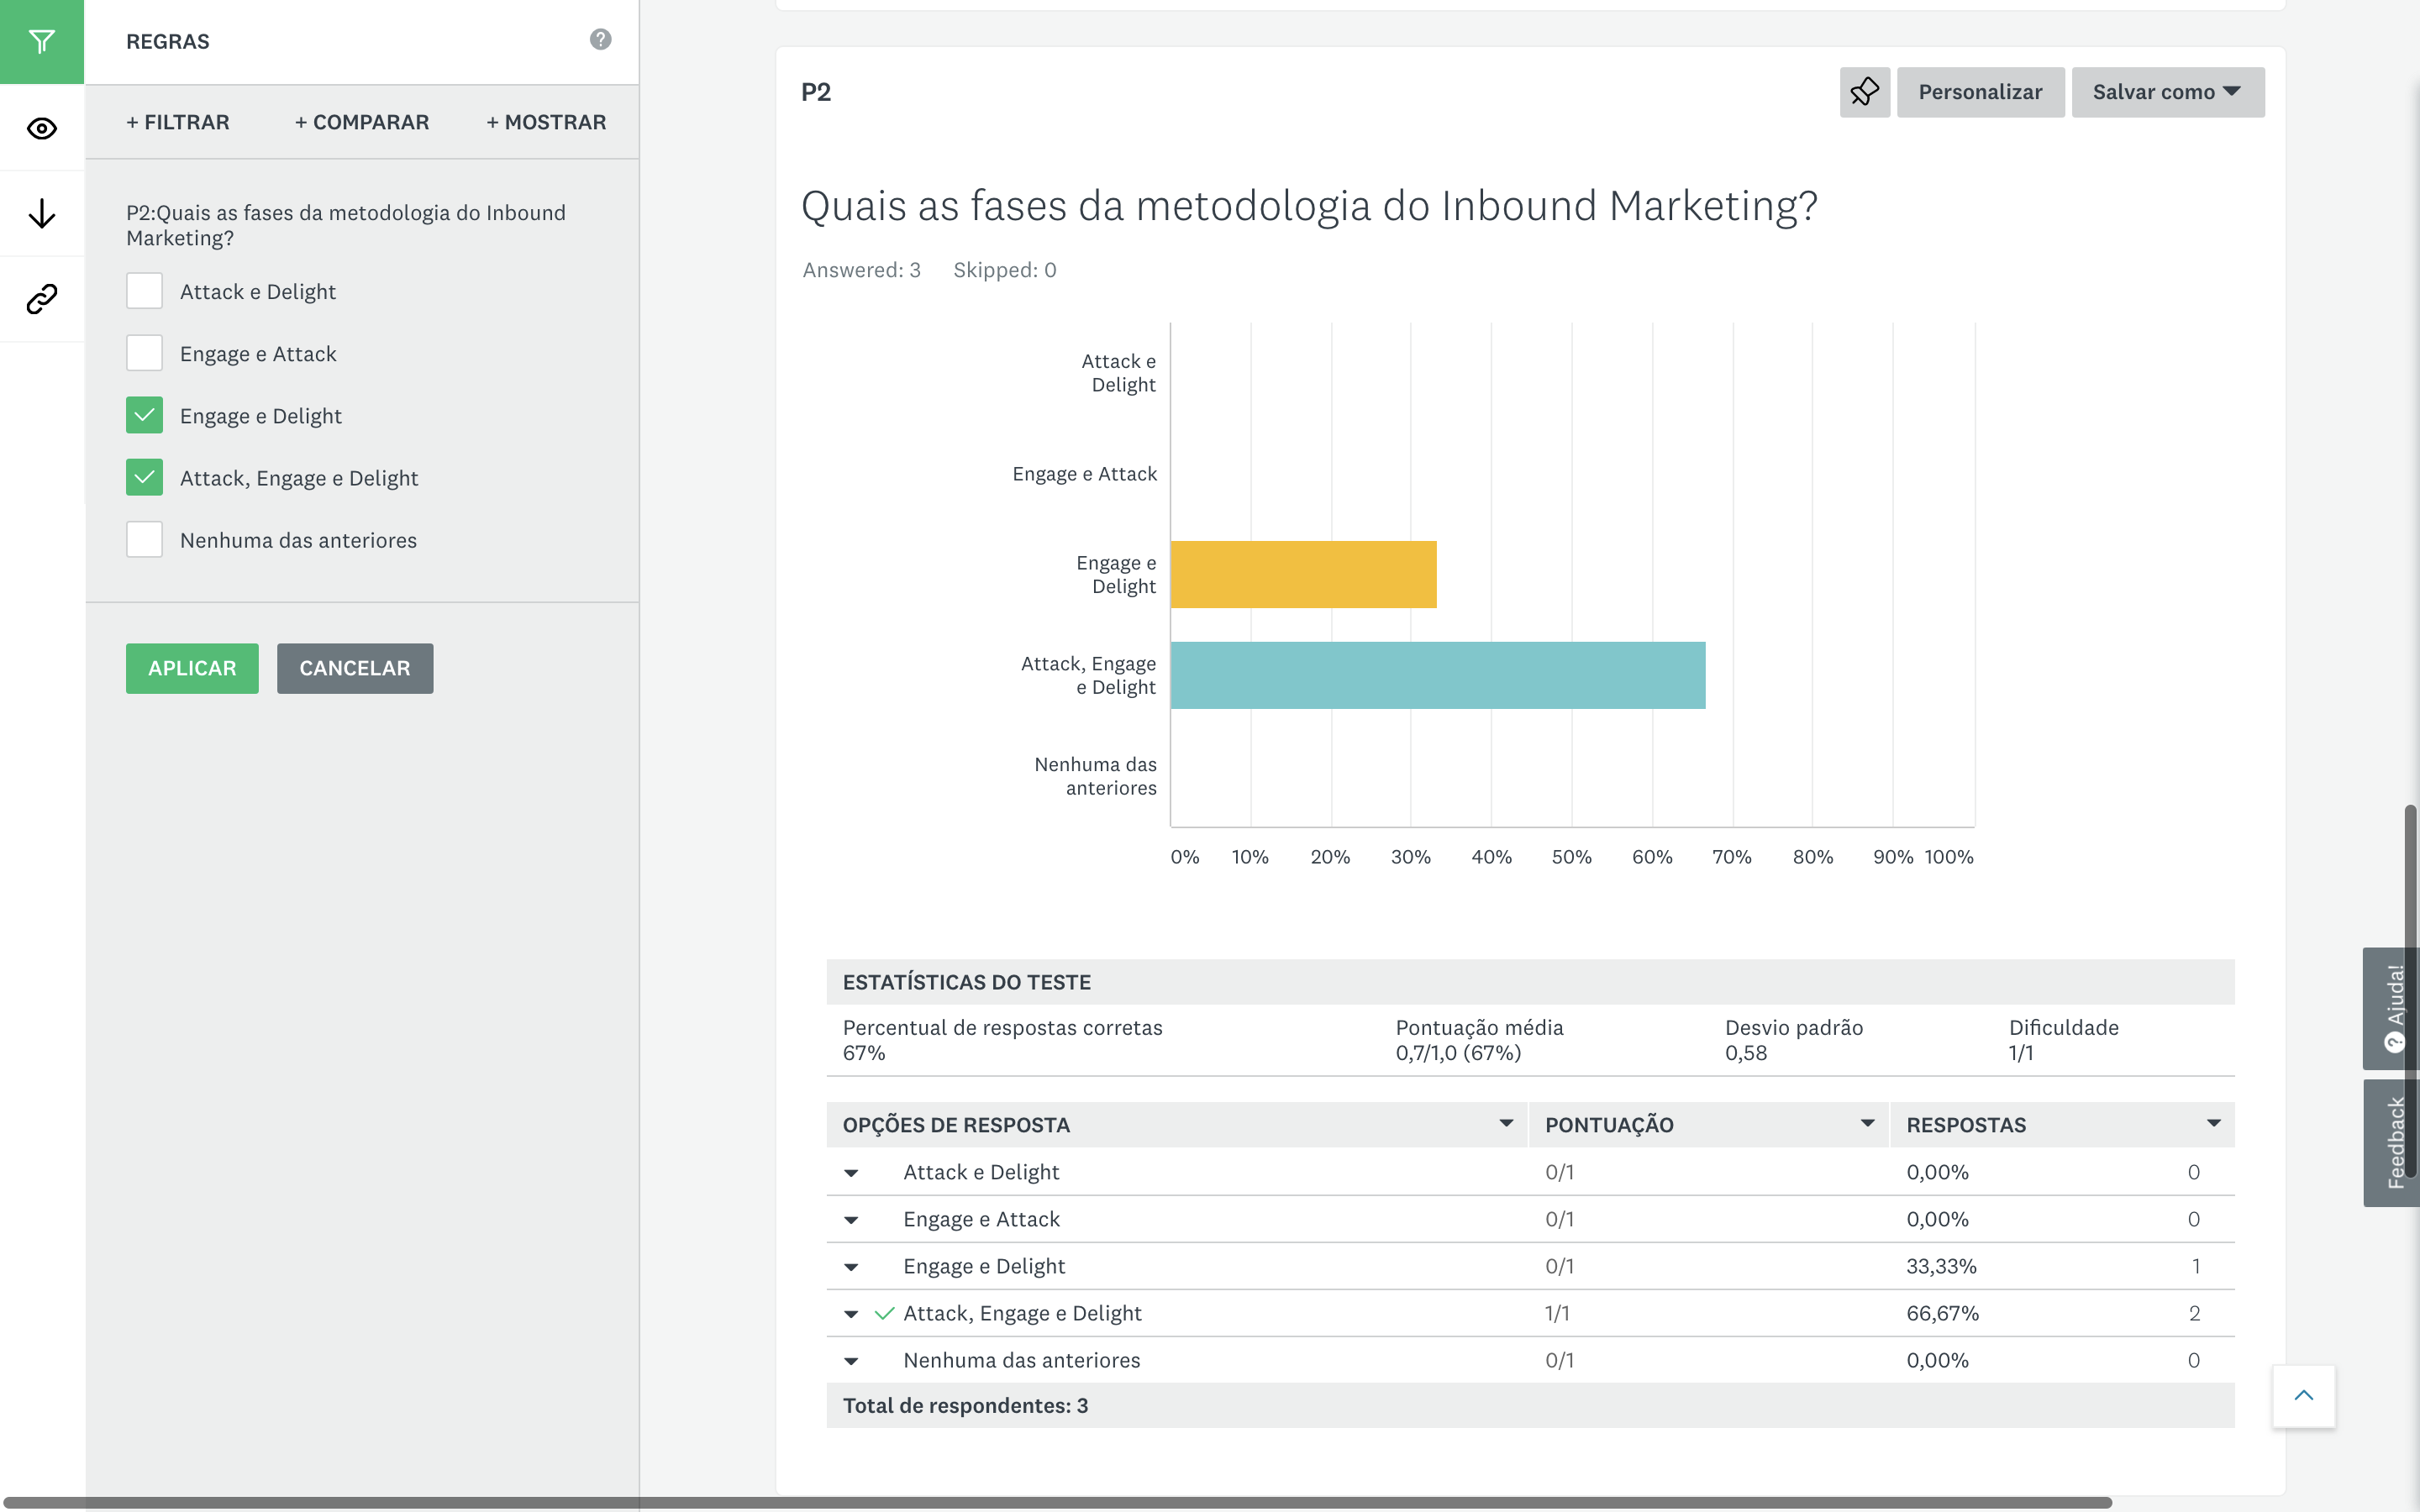
\includegraphics[width=1\textwidth]{img/sm/surveymonkey-form-filtro1}
		\caption{SurveyMonkey - Filtro aplicado na pergunta 2 }
		\label{fig:surveymonkey-form-filtro1}
	\end{center}
\end{figure}

Para finalizar a plataforma SurveyMonkey tem ainda uma funcionalidade que, através da representação dos dados numa linha temporal, permite o utilizador perceber as tendências dos dados.

\section{Typeform}
\label{typeform}

O Typeform é uma plataforma \acrshort{saas} de criação de formulários online. É uma empresa que afirma resolver o problema dos formulários e inquéritos aborrecidos e tem também como proposta de valor o facto de conseguir criar formulários e inquéritos sem ter que programar uma única linhad e código. Esta plataforma permite recolher informações do público alvo através de formulários e inquéritos personalizados e no final visualizar estes dados. 

O Typeform disponilibilisa um pacote gratuito, contudo, é necessário criar conta de utilizador, para aceder ás funcionalidades da plataforma. Tanto o registro como o início de sessão pode ser feito através da \acrfull{api} do Google.

Como podemos ver na Figura \ref{fig:tf-dashboard}, no painel de controlo, podemos criar várias áreas de trabalho. Cada área de trabalho é independente e todos os formulários e inquéritos que forem adicionados ao mesmo podem ser partilhados com mais do que uma pessoa.

\clearpage

\begin{figure}[ht!]
	\begin{center}
		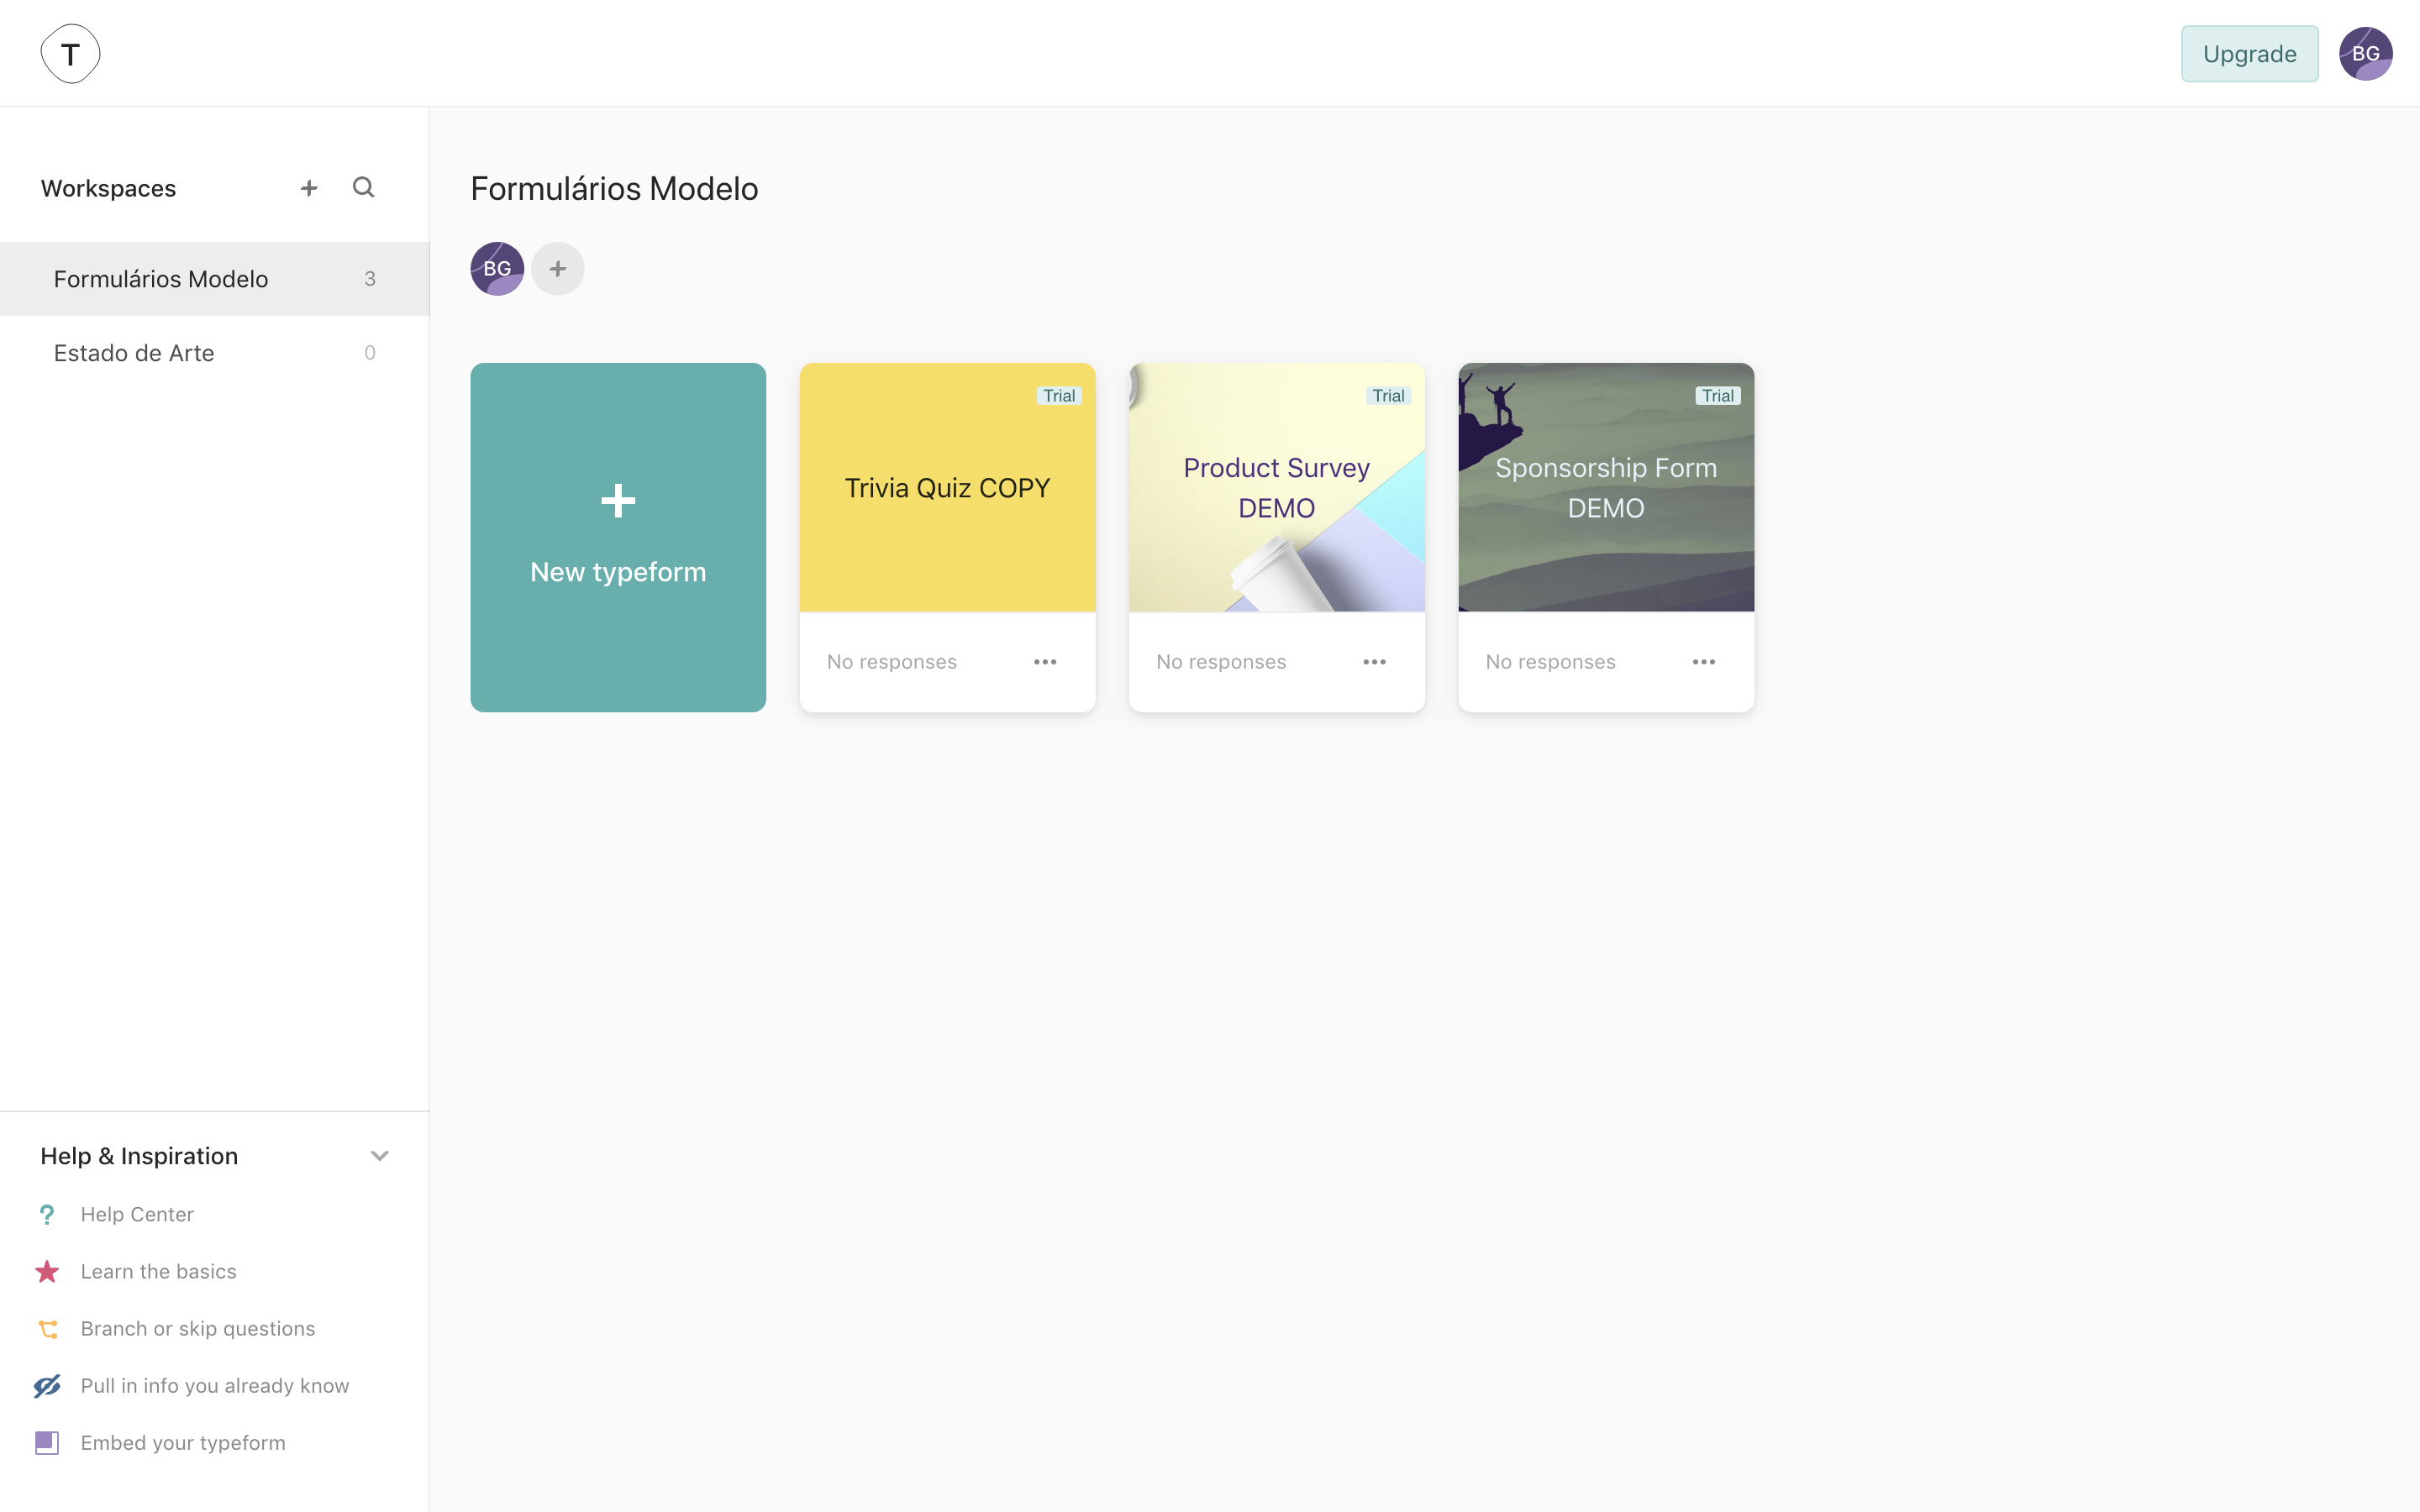
\includegraphics[width=1\textwidth]{img/tf/tf-dashboard}
		\caption{Typeform - Painel de Controlo}
		\label{fig:tf-dashboard}
	\end{center}
\end{figure}

Na criação de um formulário ou inquérito, do zero, a plataforma lista uma séria de templates que se podem filtrar por categorias na coluna à esquerda, como se pode observar na Figura \ref{fig:tf-form-create}.

\begin{figure}[ht!]
	\begin{center}
		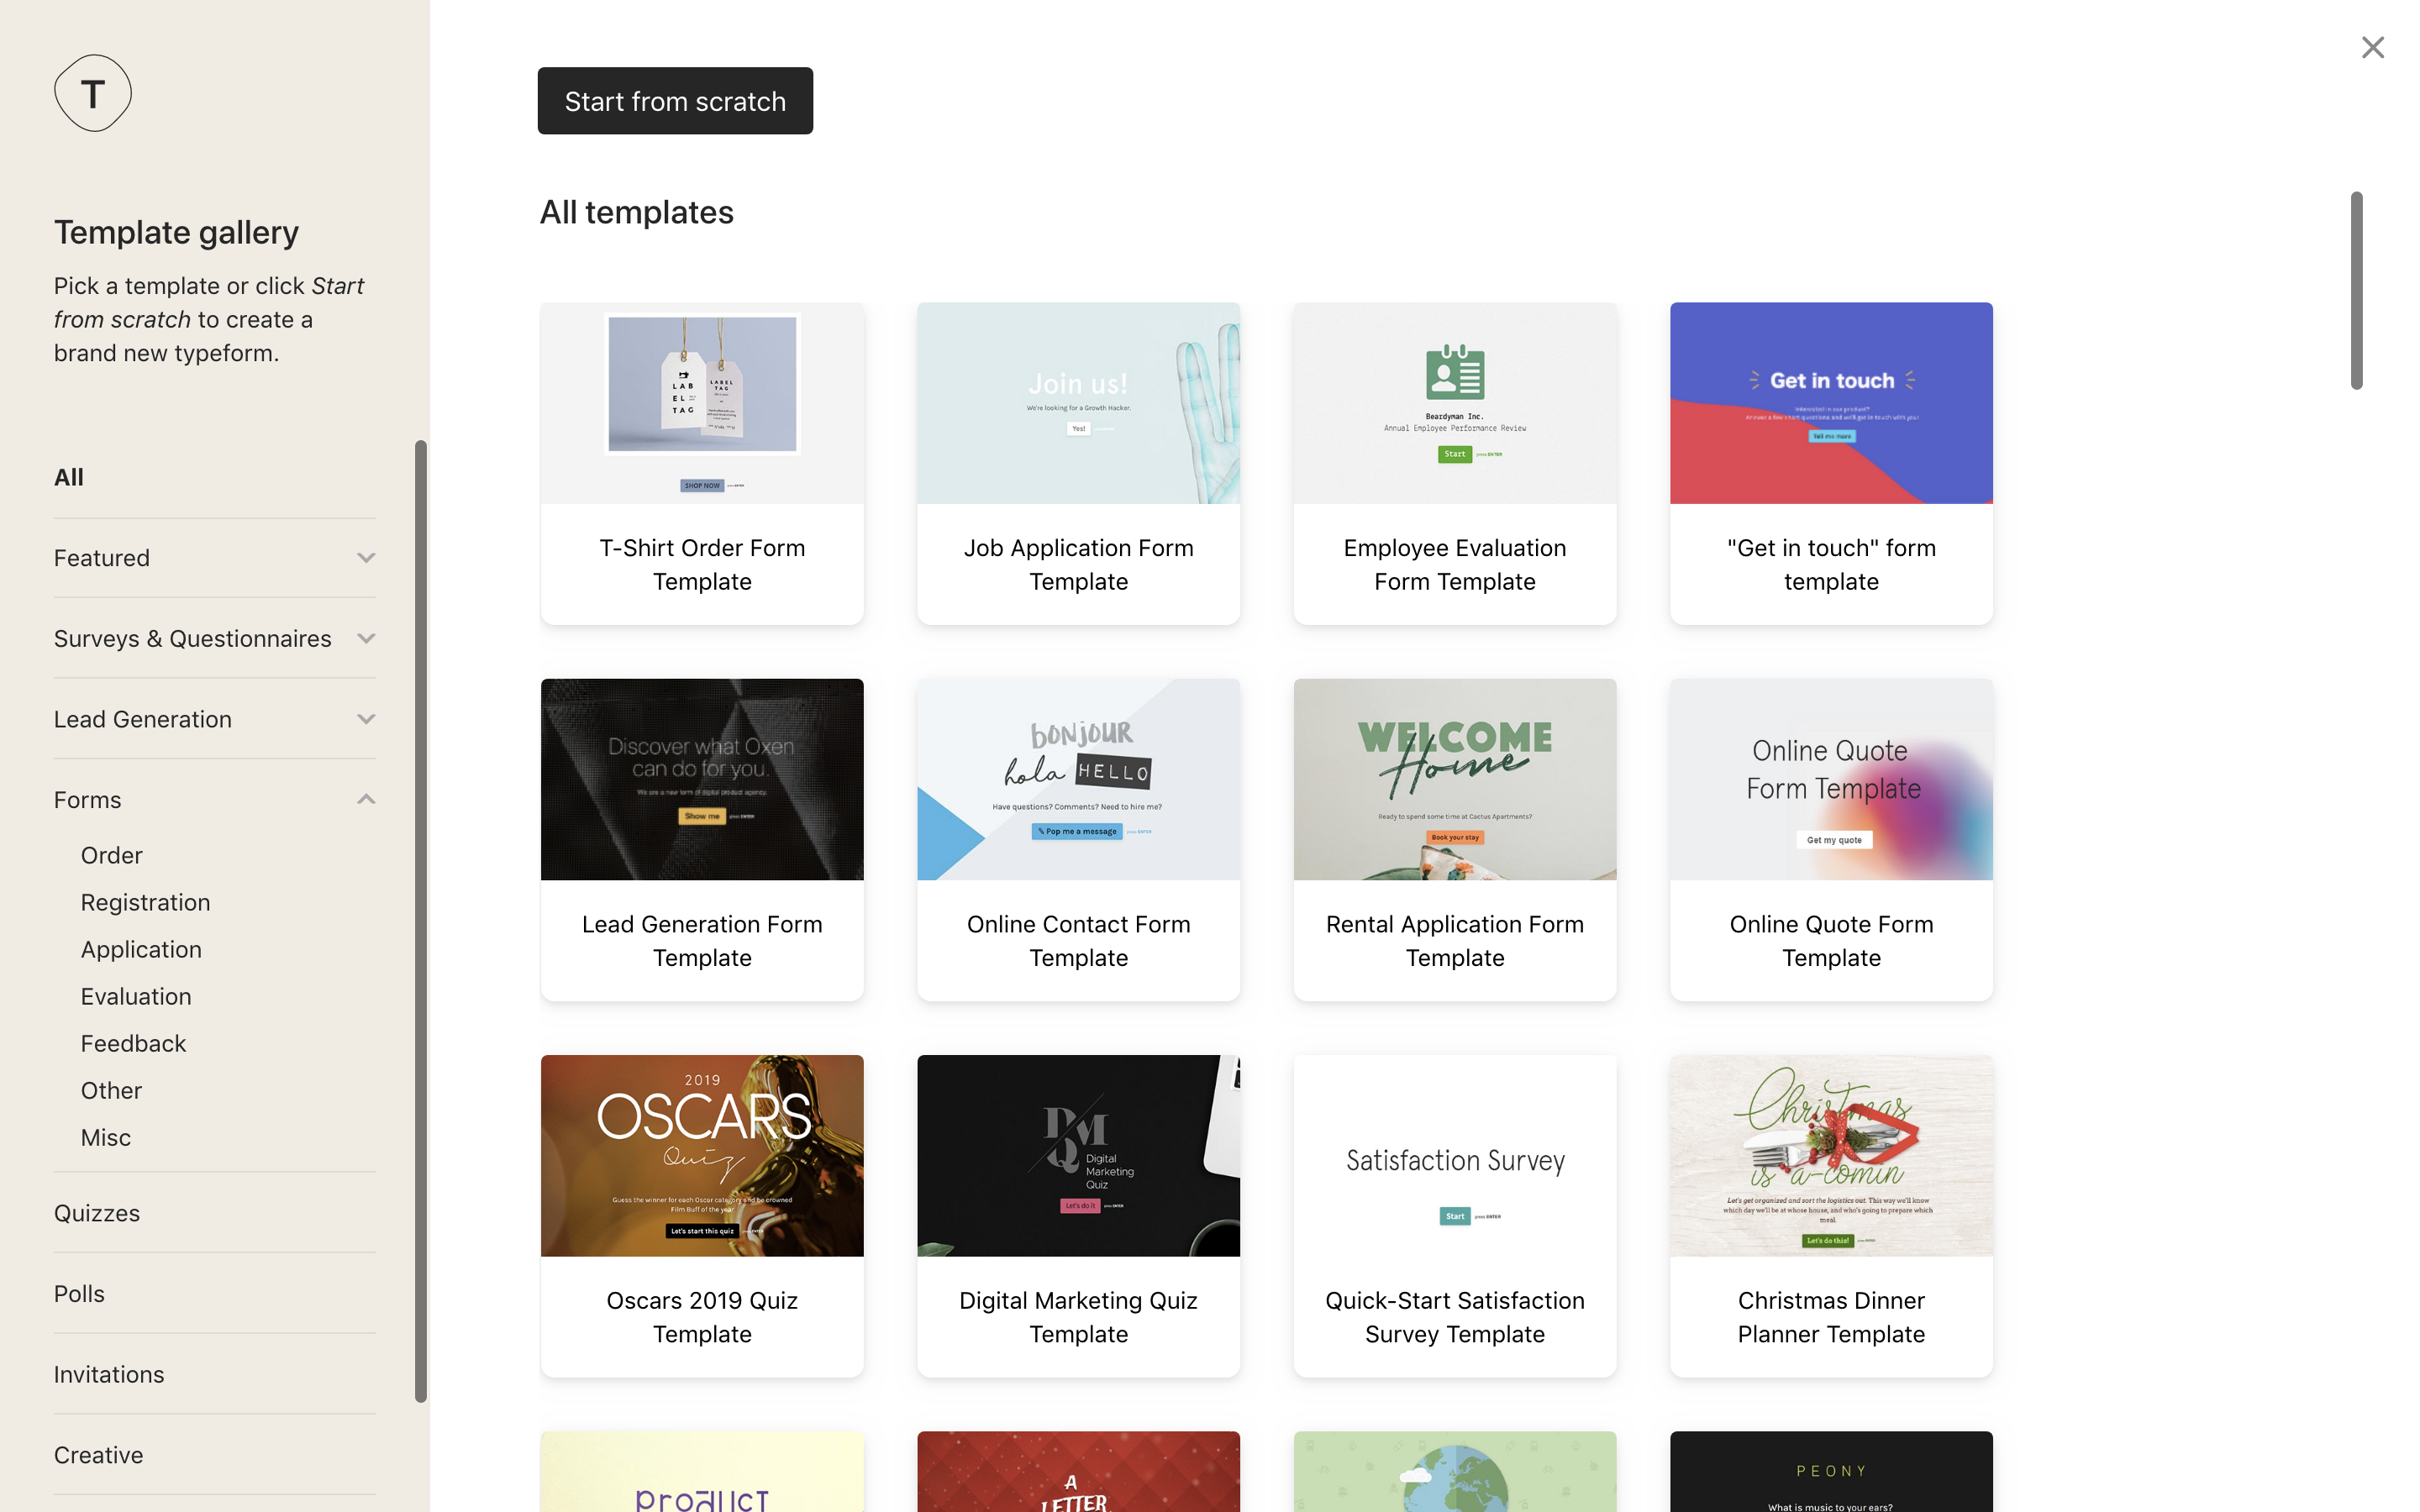
\includegraphics[width=1\textwidth]{img/tf/tf-form-create}
		\caption{Typeform - Criar Formulário}
		\label{fig:tf-form-create}
	\end{center}
\end{figure}
\newpage

\begin{figure}[ht!]
	\begin{center}
		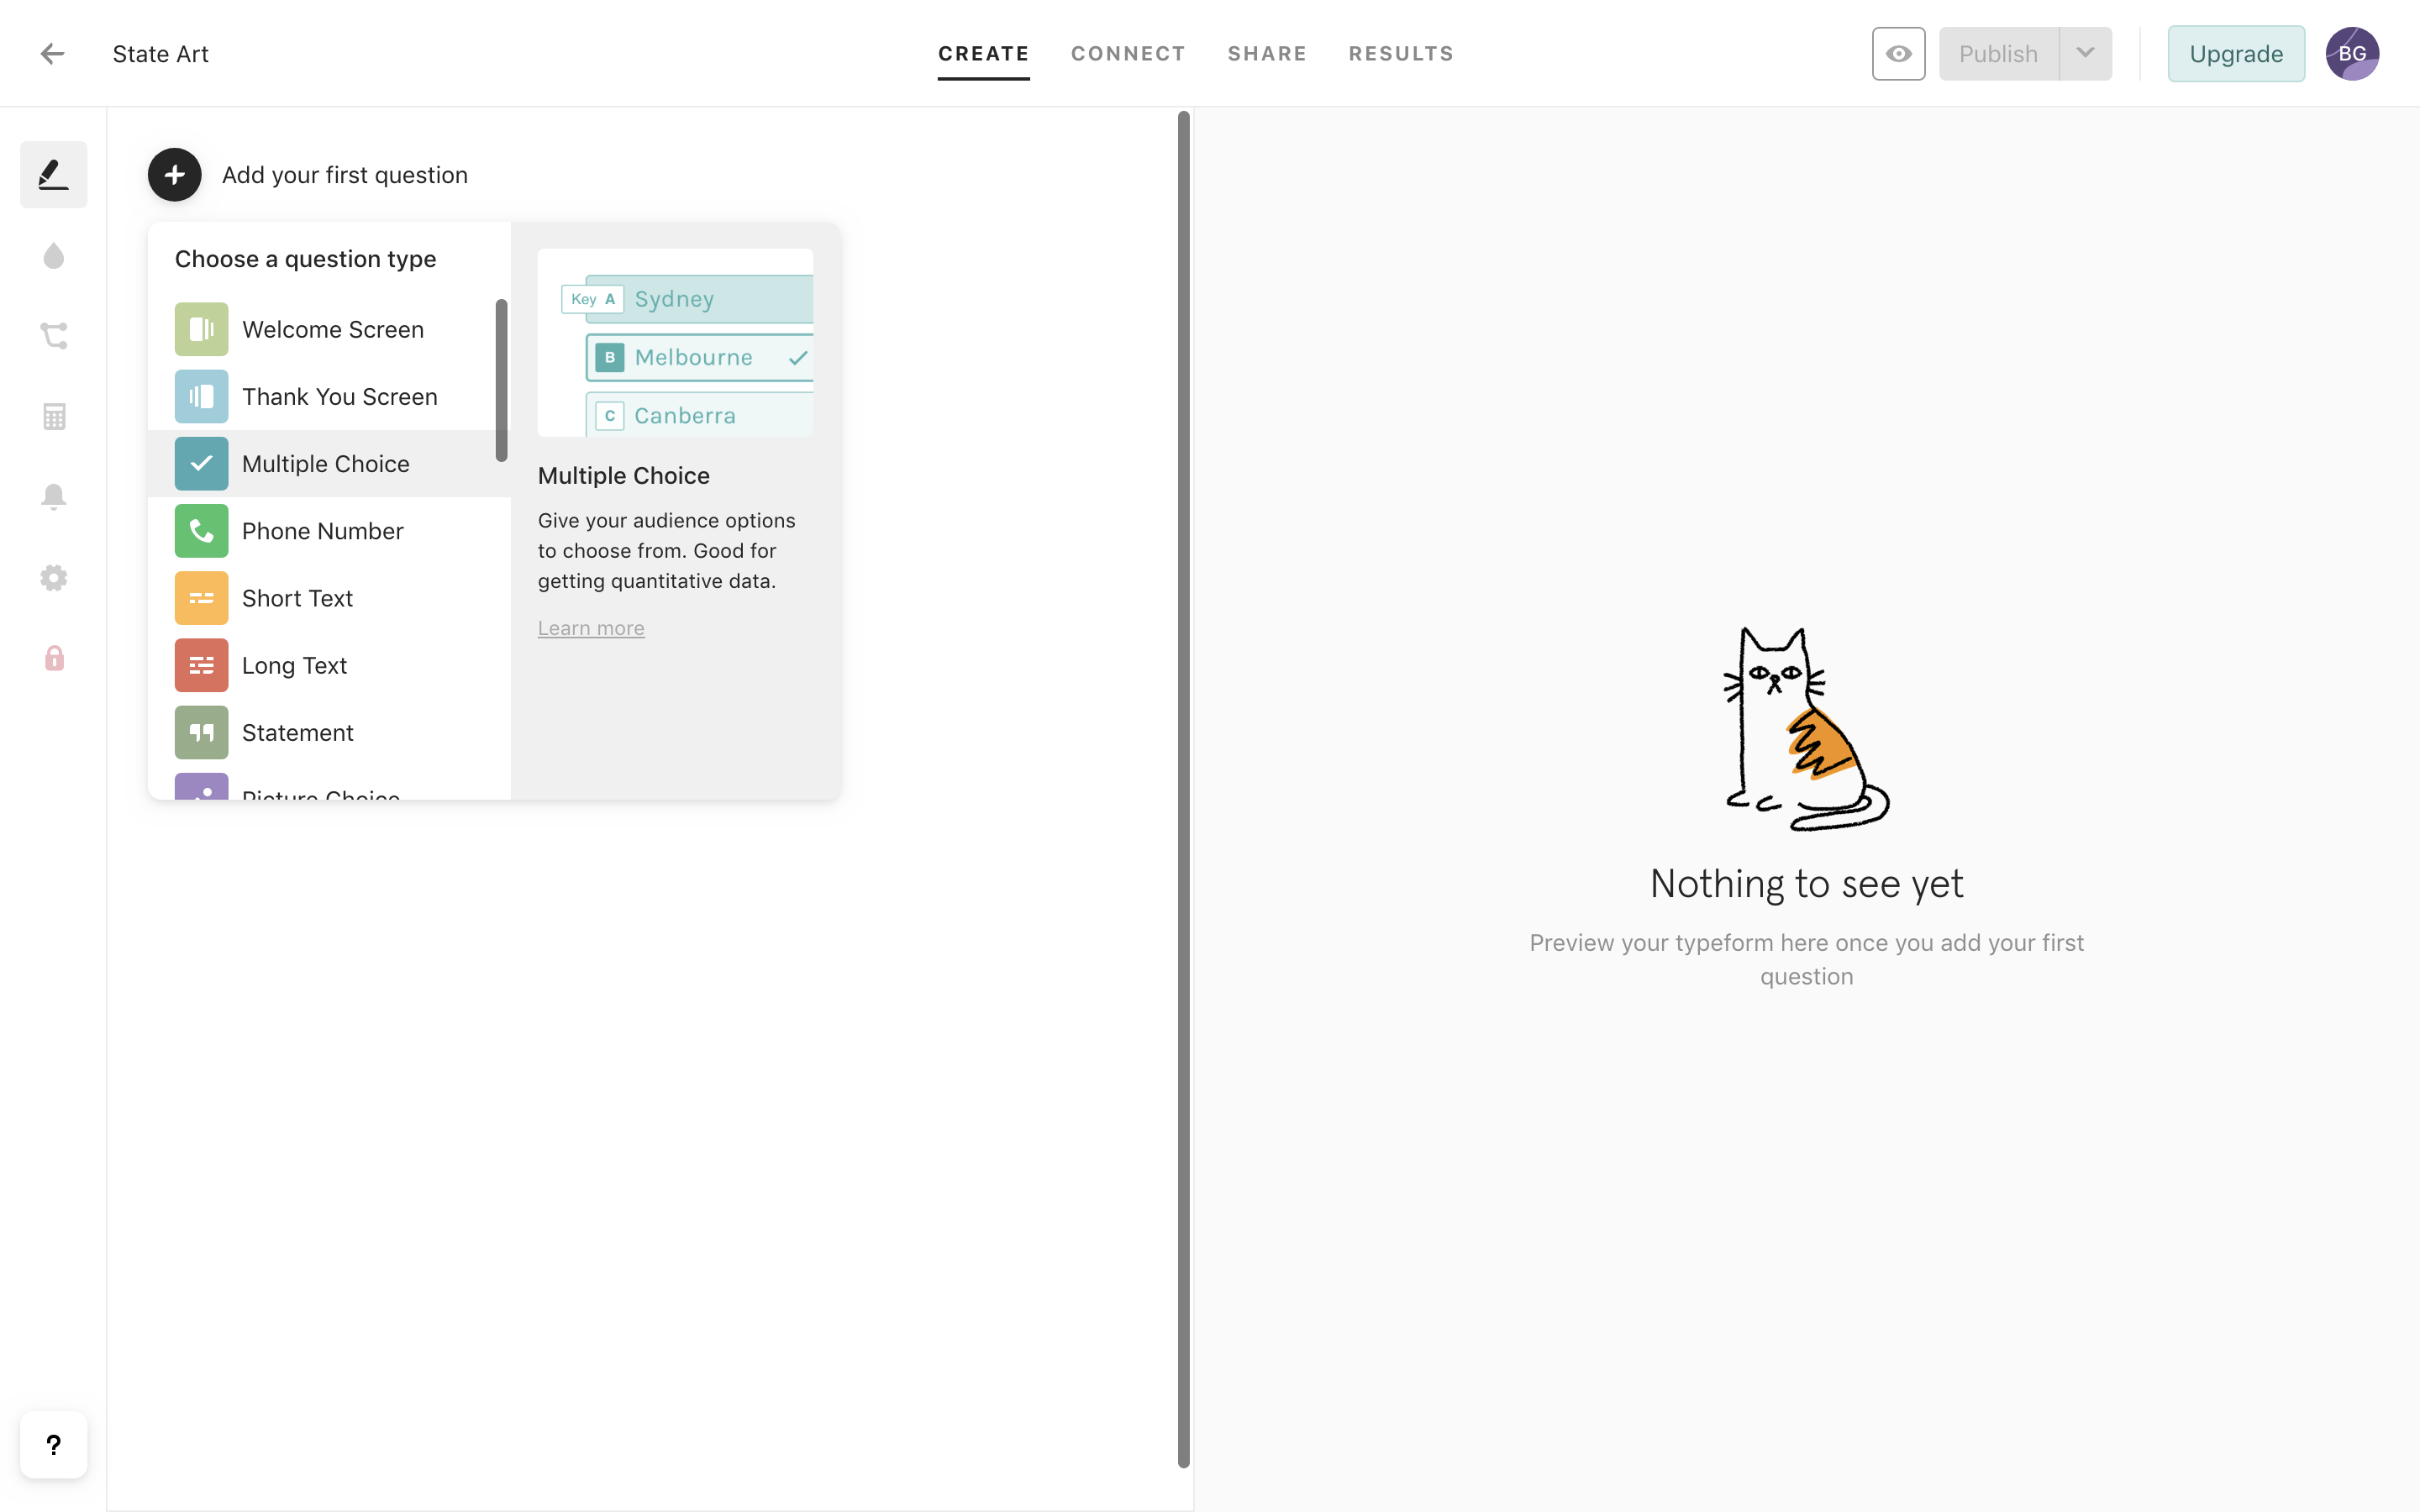
\includegraphics[width=1\textwidth]{img/tf/tf-question-type}
		\caption{Typeform - Tipos de pergunta}
		\label{fig:tf-question-type}
	\end{center}
\end{figure}

Representado na Figura \ref{fig:tf-question-type} temos os tipos de pergunta que a plataforma permite adicionar no formulário. Estas perguntas podem ser personalizaveis tanto a nível estético como funcional como podemos ver nas Figuras \ref{fig:tf-question-opcoes} e \ref{fig:tf-question-custom}, respectivamente. É também possível criar um tema novo para cada pergunta onde se pode escolher a fonte de texto, imagem de fundo e cores da pergunta, respostas, butões e fundo.

\begin{figure}[ht!]
	\begin{center}
		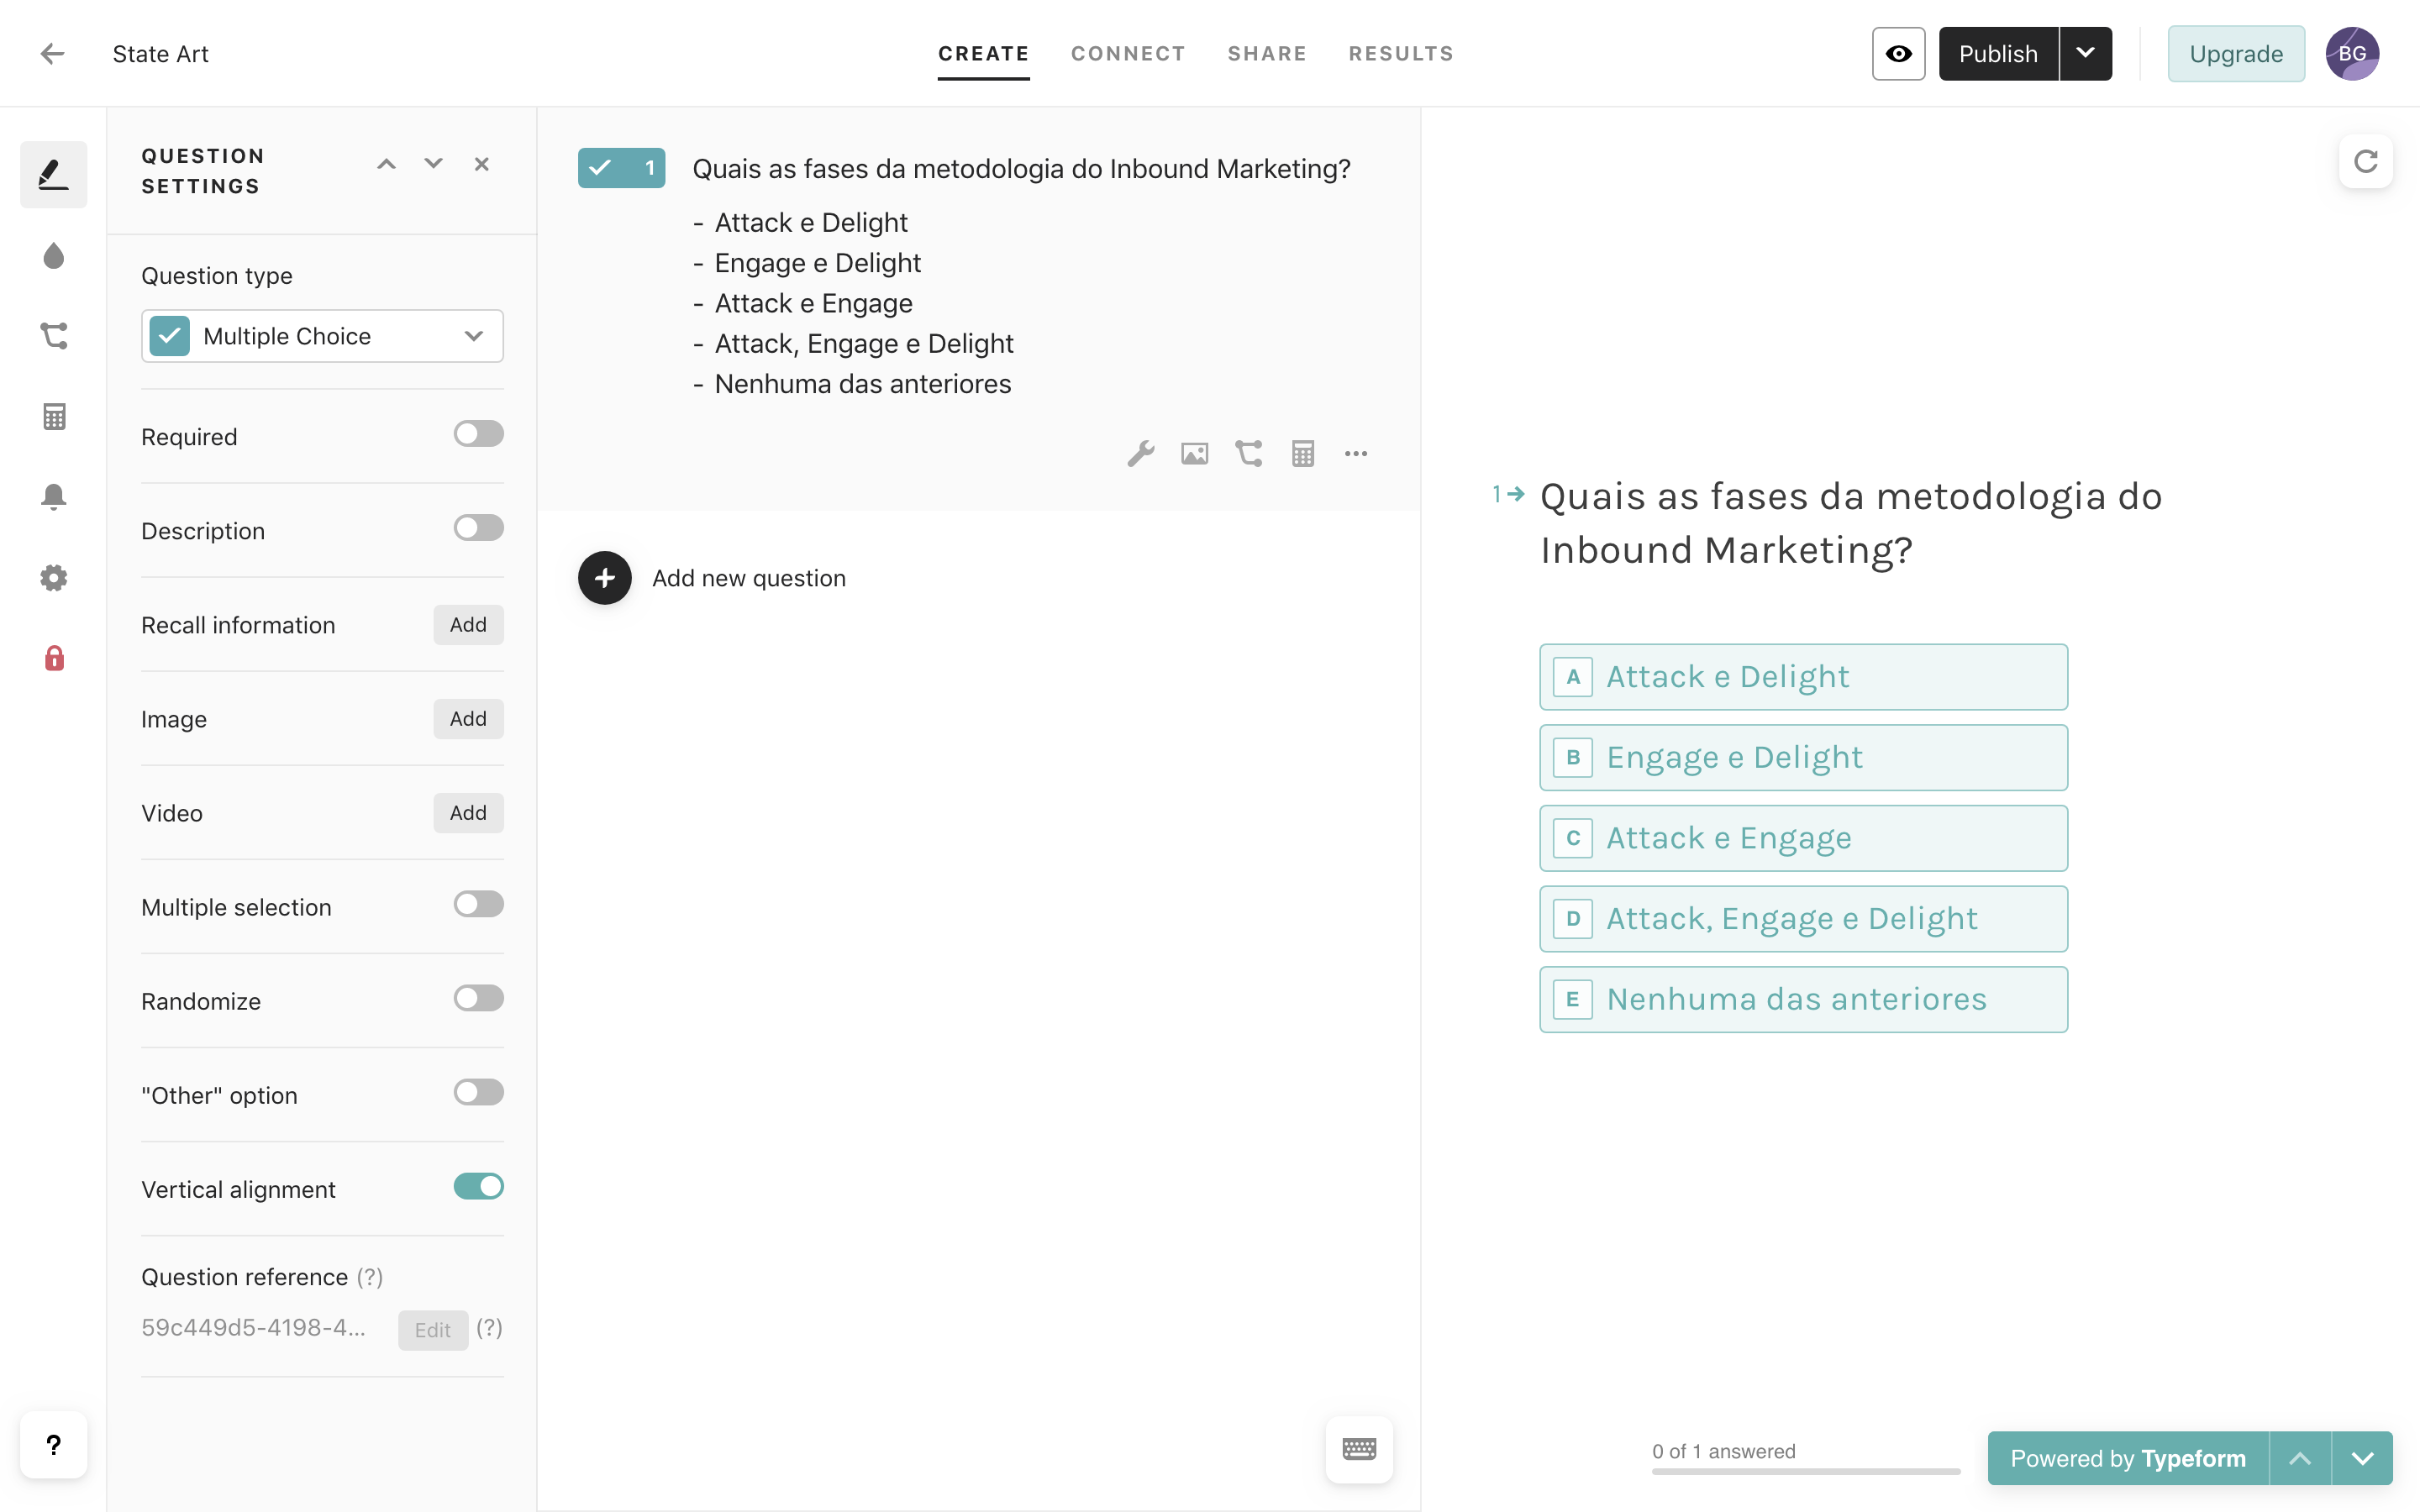
\includegraphics[width=1\textwidth]{img/tf/tf-question-opcoes}
		\caption{Typeform - Opções da pergunta}
		\label{fig:tf-question-opcoes}
	\end{center}
\end{figure}

\begin{figure}[ht!]
	\begin{center}
		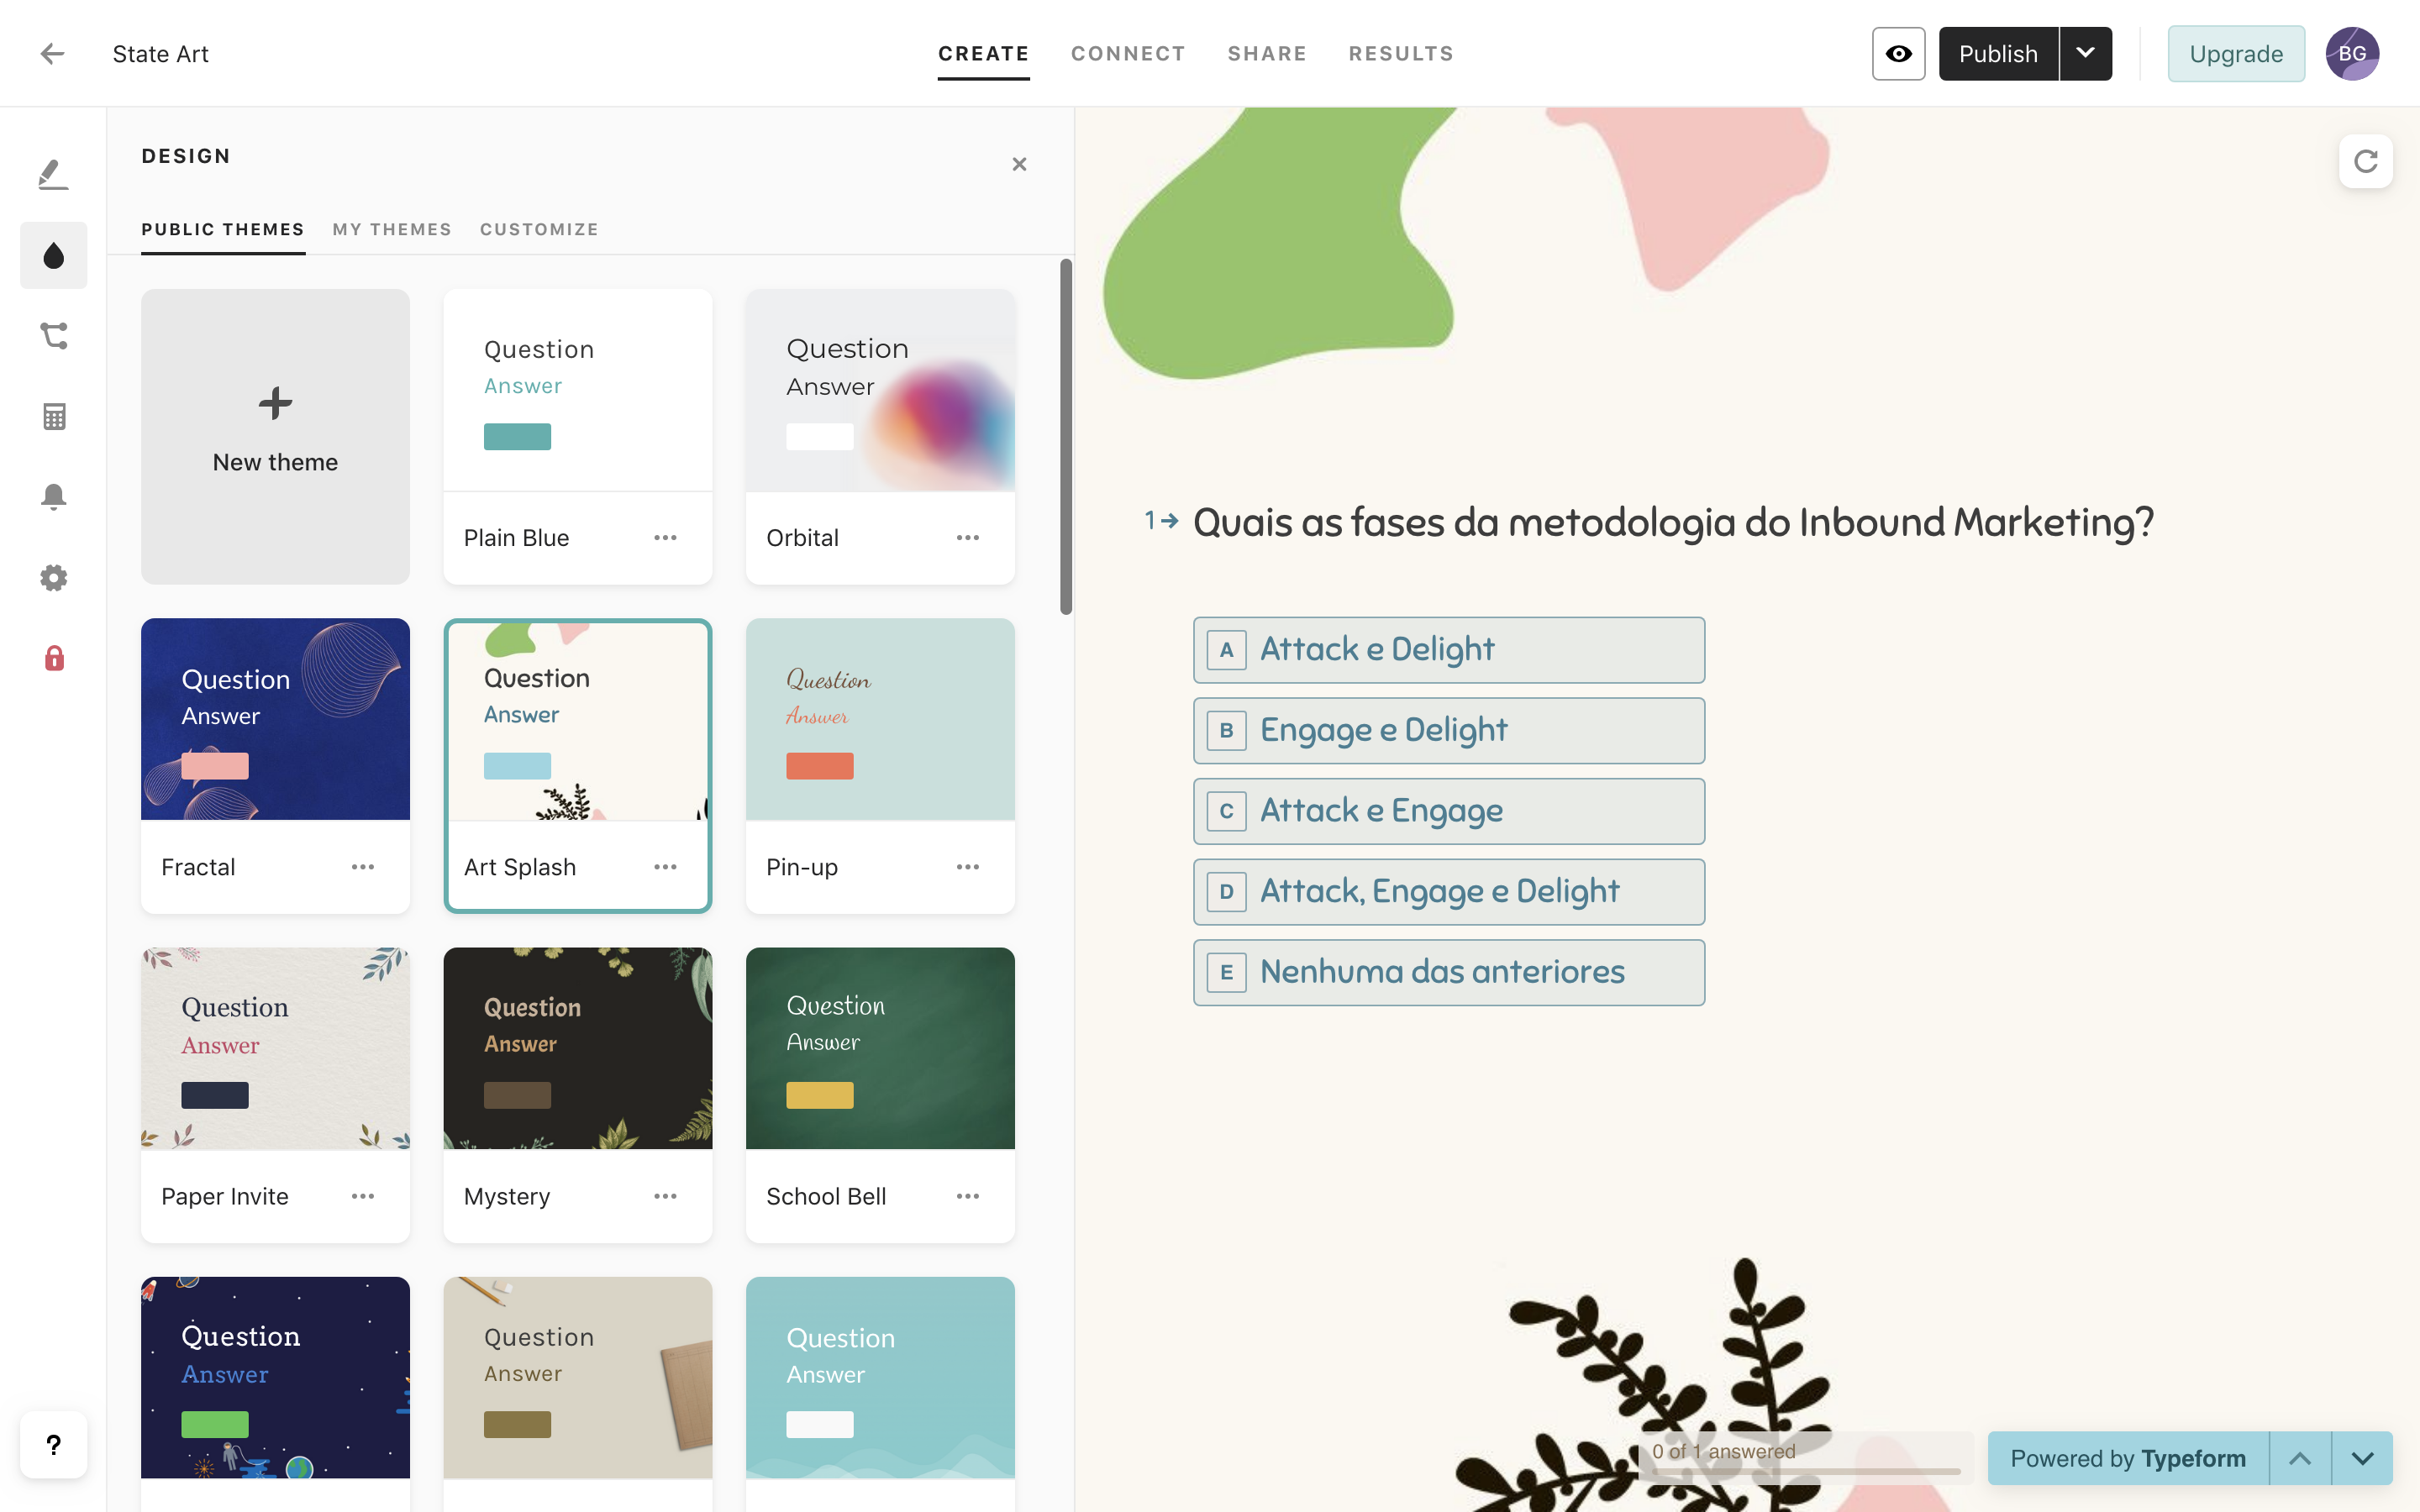
\includegraphics[width=1\textwidth]{img/tf/tf-question-custom}
		\caption{Typeform - Design da pergunta}
		\label{fig:tf-question-custom}
	\end{center}
\end{figure}

A plataforma permite ainda os utilizadores adicionarem lógicas aos seus formulário, como exemplificado na Figura \ref{fig:tf-question-logica} , em que caso a resposta à pergunta 4 seja a especificada, o caminho a tomar será diferente. 



\begin{figure}[ht!]
	\begin{center}
		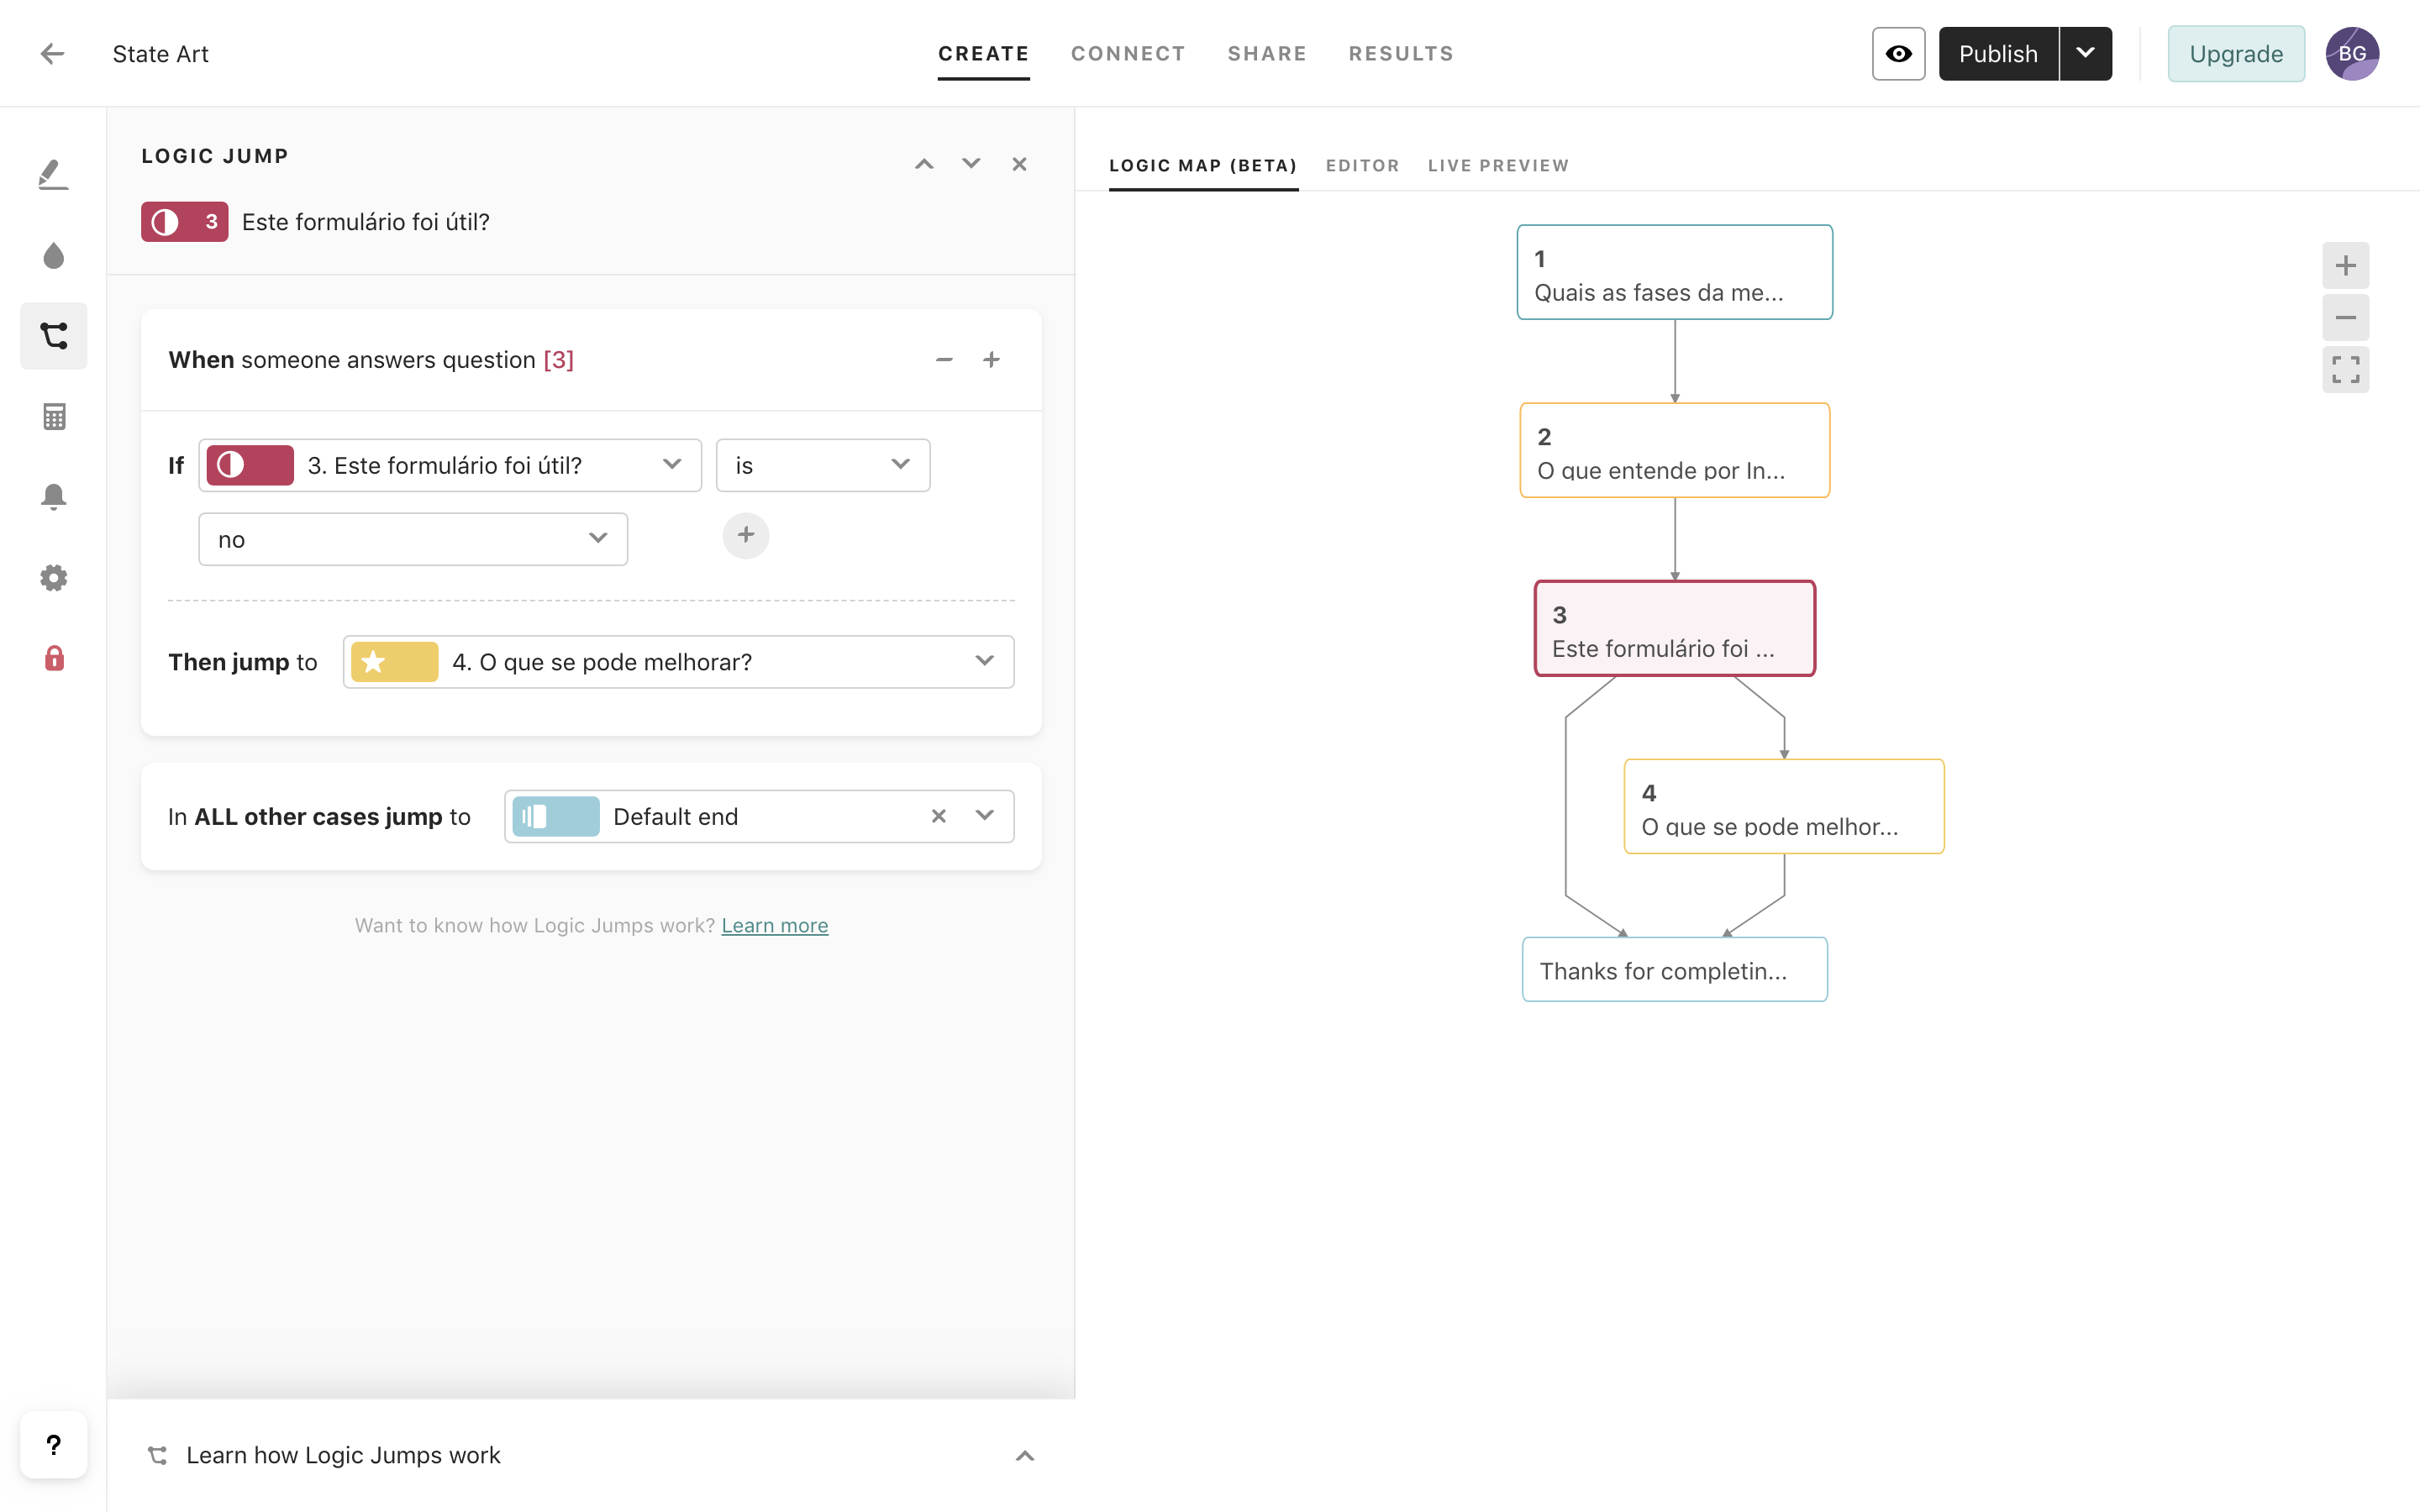
\includegraphics[width=1\textwidth]{img/tf/tf-question-logica}
		\caption{Typeform - Lógica do formulário}
		\label{fig:tf-question-logica}
	\end{center}
\end{figure}

\newpage

A funcionalidade de visualizar o formulário está disponivel no canto superior direito, no lado esquerdo do botão de publicar, que permite o autor verificar se tudo está feito conforme planeado e assim poder publicar e partilhar.

O Typeform permite também a integração de serviços externos com o formulário, como podemos ver na Figura \ref{fig:tf-question-integration} , em que, por exemplo, utilizando o Google Sheets\cite{googlesheets}, os resultados são exportados directamente para uma \textit{google sheet}


\begin{figure}[ht!]
	\begin{center}
		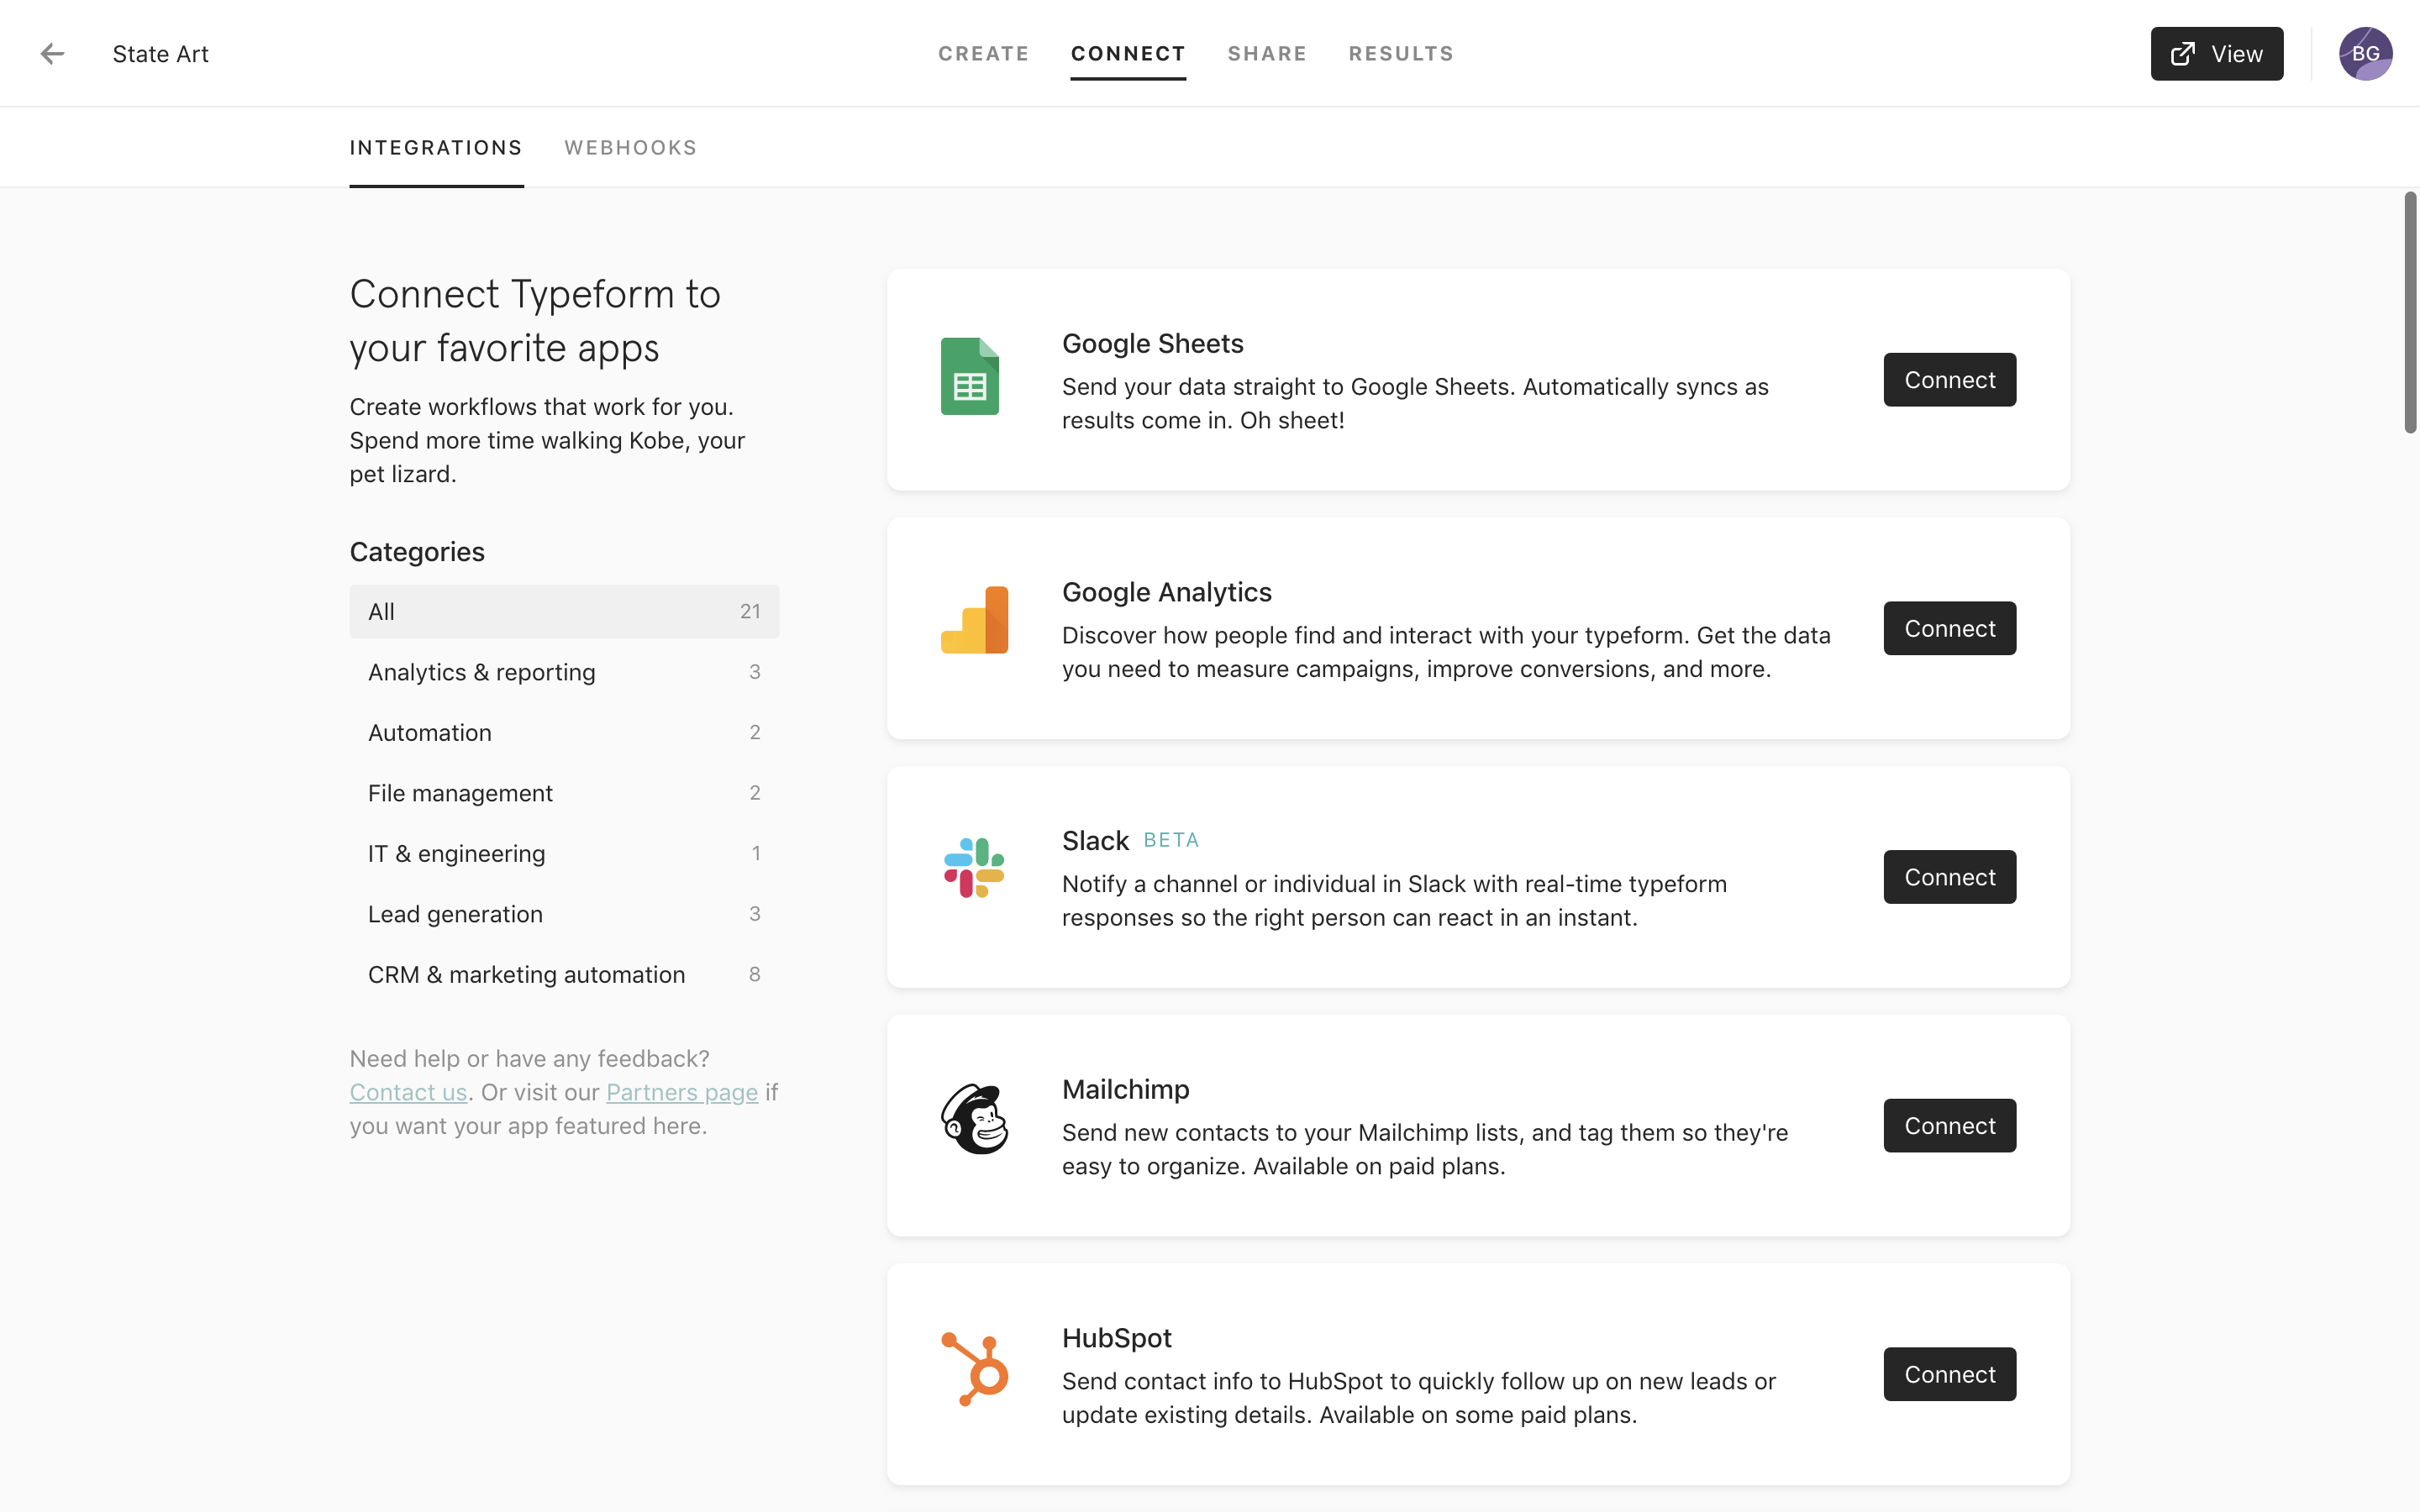
\includegraphics[width=1\textwidth]{img/tf/tf-question-integration}
		\caption{Typeform - Integração com sistemas externos}
		\label{fig:tf-question-integration}
	\end{center}
\end{figure}

Representado na Figura \ref{fig:tf-question-results} , temos a secção de analise de dados da plataforma onde podemos ver uma sumarização dos dados recebidos ou  analisar todas as respostas uma a uma. É também possível gerar um reportório dos dados recebidos e partilhar com alguém em qualquer fase, por exemplo, de uma campanha, uma vez que o mesmo é actualizado automaticamente com as novas respostas recebidas. 

O Typeform não fornece quaisquer filtros para segmentar os dados, contudo, fora as respostas em si, exibe algumas estatísticas/métricas relacionadas com os dispositivos que foram utilizados para responder aos formulários.


\newpage
\begin{figure}[ht!]
	\begin{center}
		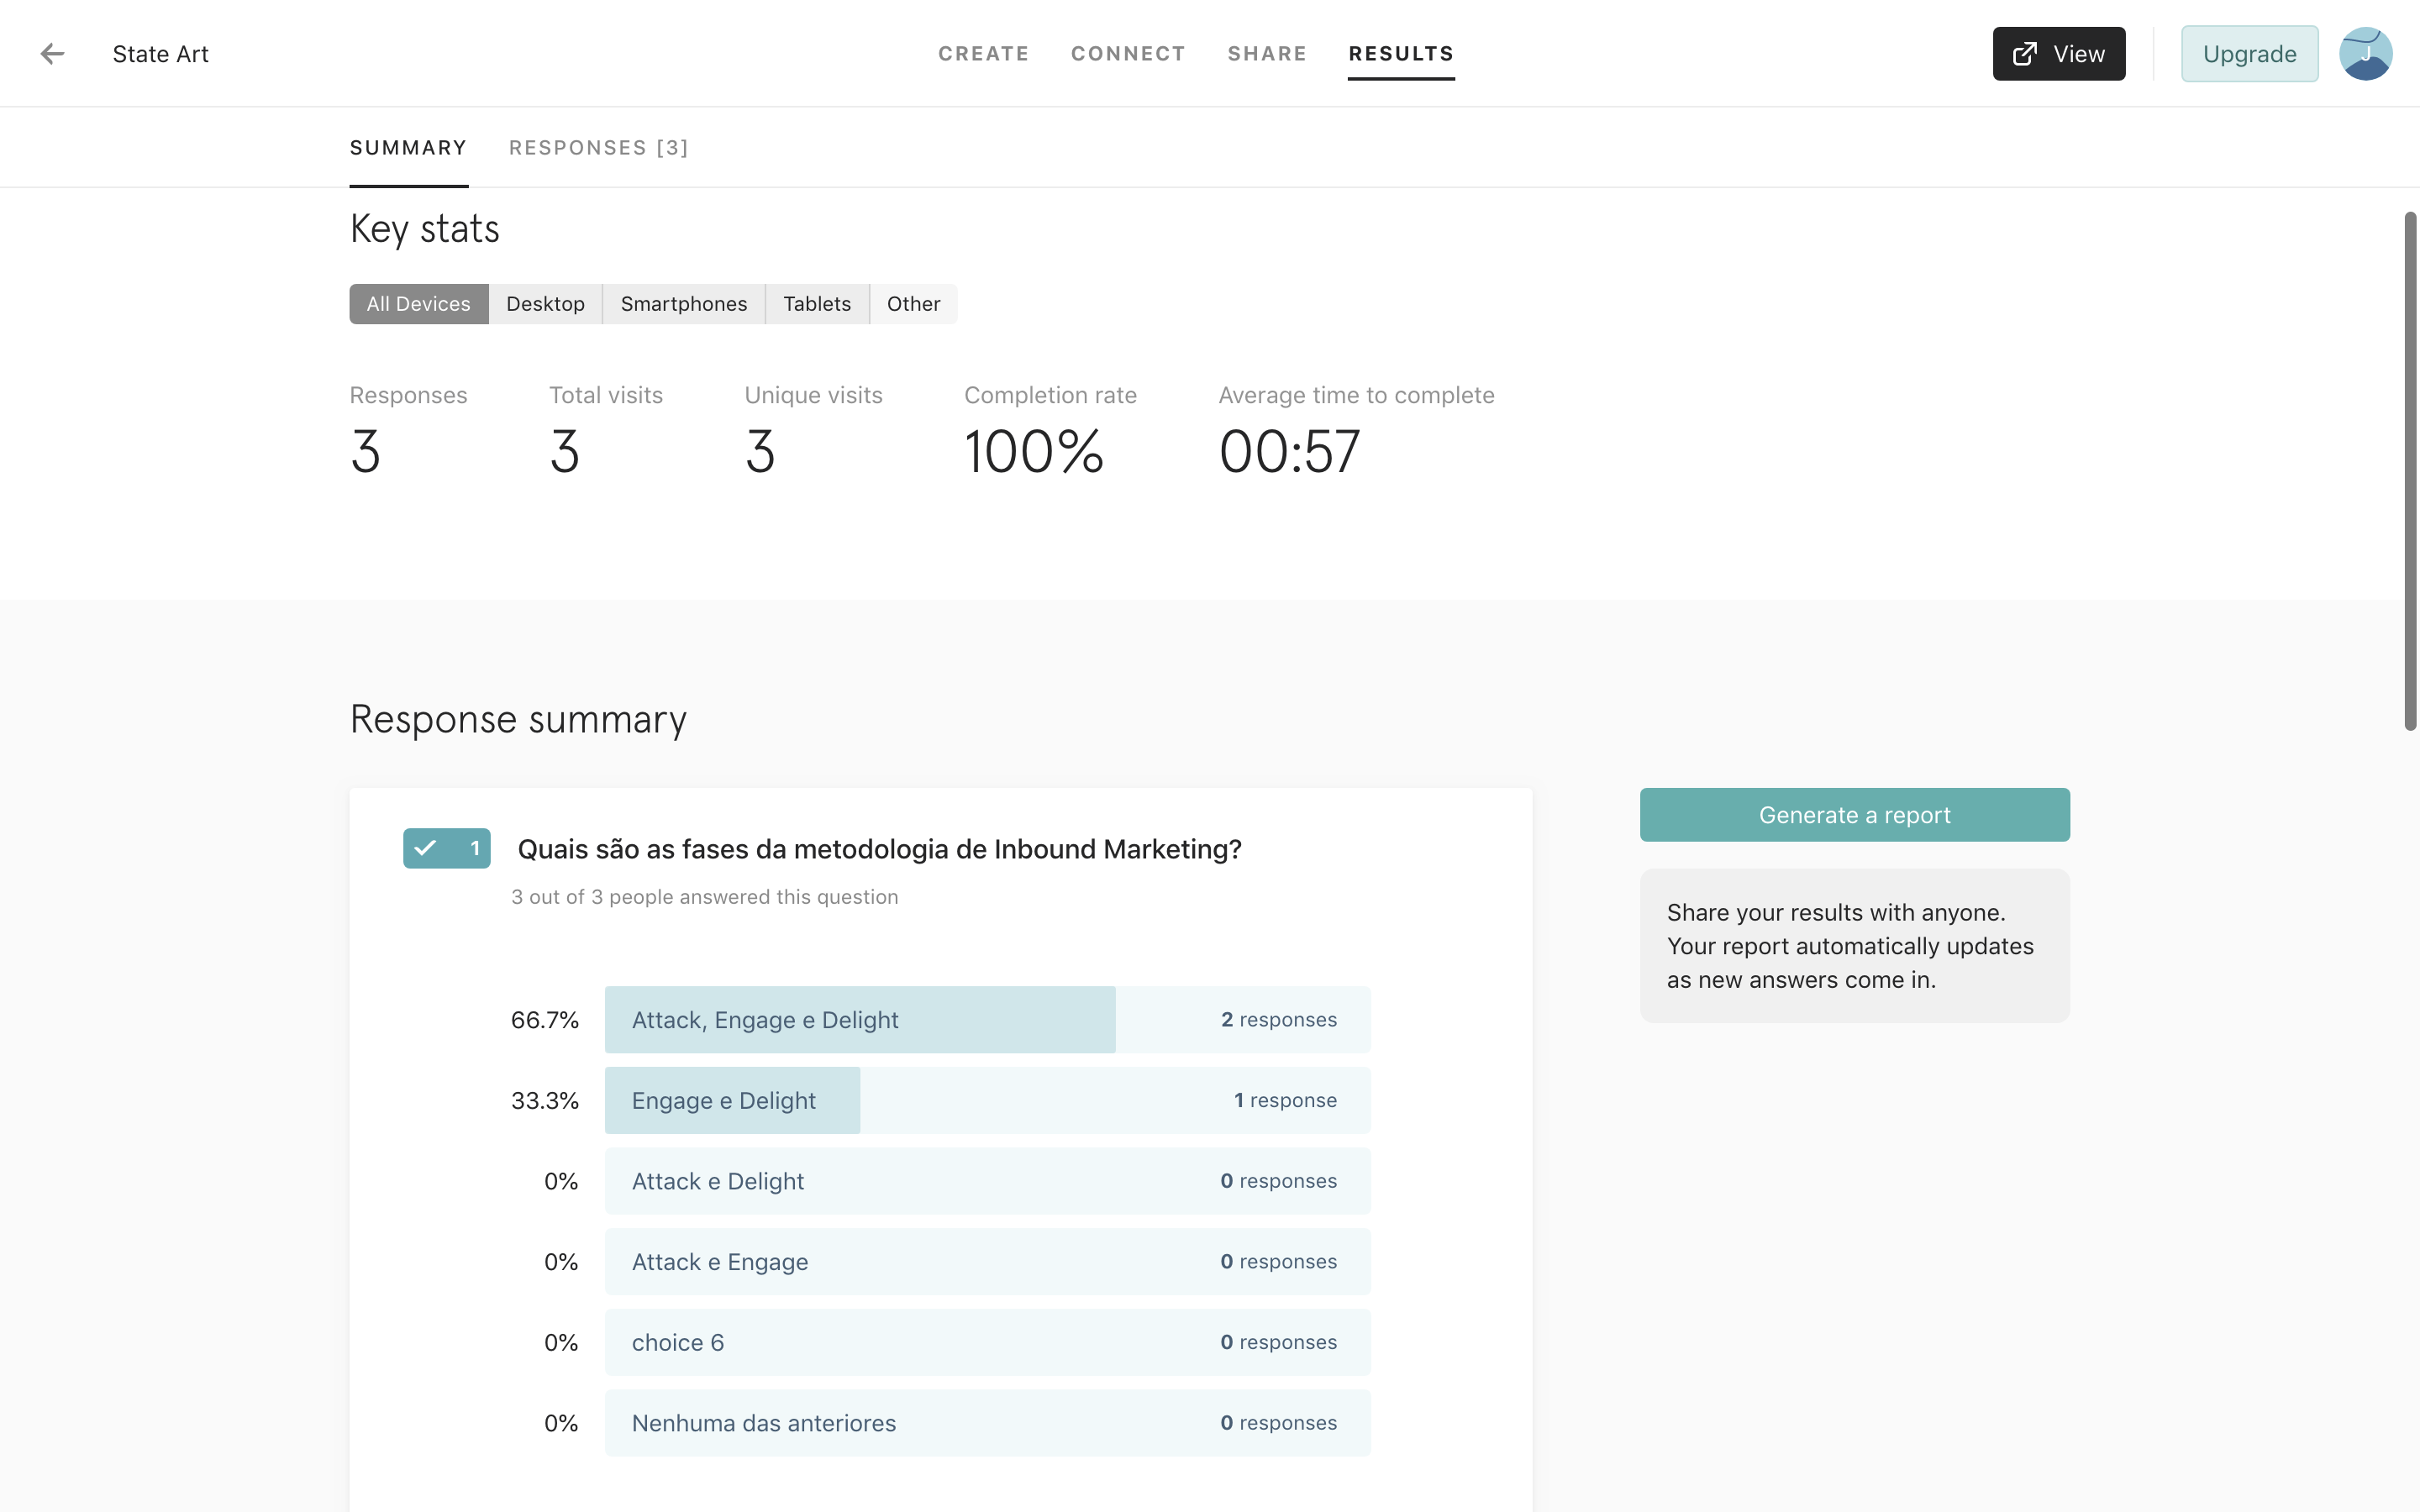
\includegraphics[width=1\textwidth]{img/tf/tf-question-results}
		\caption{Typeform - Analise de resultados}
		\label{fig:tf-question-results}
	\end{center}
\end{figure}

\section{Google Form}
\label{googleform}

O Google Form é uma aplicação de adminstração de inquéritos que está incluída no Google Drive office juntamente com o Google Docs\cite{gdocs}, Google Sheets e Google Slides\cite{gslides}. Esta ferramenta permite recolher informações do público alvo através de formulários e inquéritos personalizados e automaticamente exportar os dados para uma \textit{google sheet}.

Estam aplicação é totalmente gratuita, bastanto apenas criar uma conta Google para poder aceder a todas as funcionalidades da ferramenta.

Representado na Figura \ref{fig:gf-dashboard}, está o painel de controlo da conta de um utilizador, onde o mesmo pode visualizar os formulários com que interagiu recentemente. Por cima dos formulários recentes temos o butão para criar um novo formulário juntamente com alguns \textit{templates}/recomendações de formulários.

\newpage

\begin{figure}[ht!]
	\begin{center}
		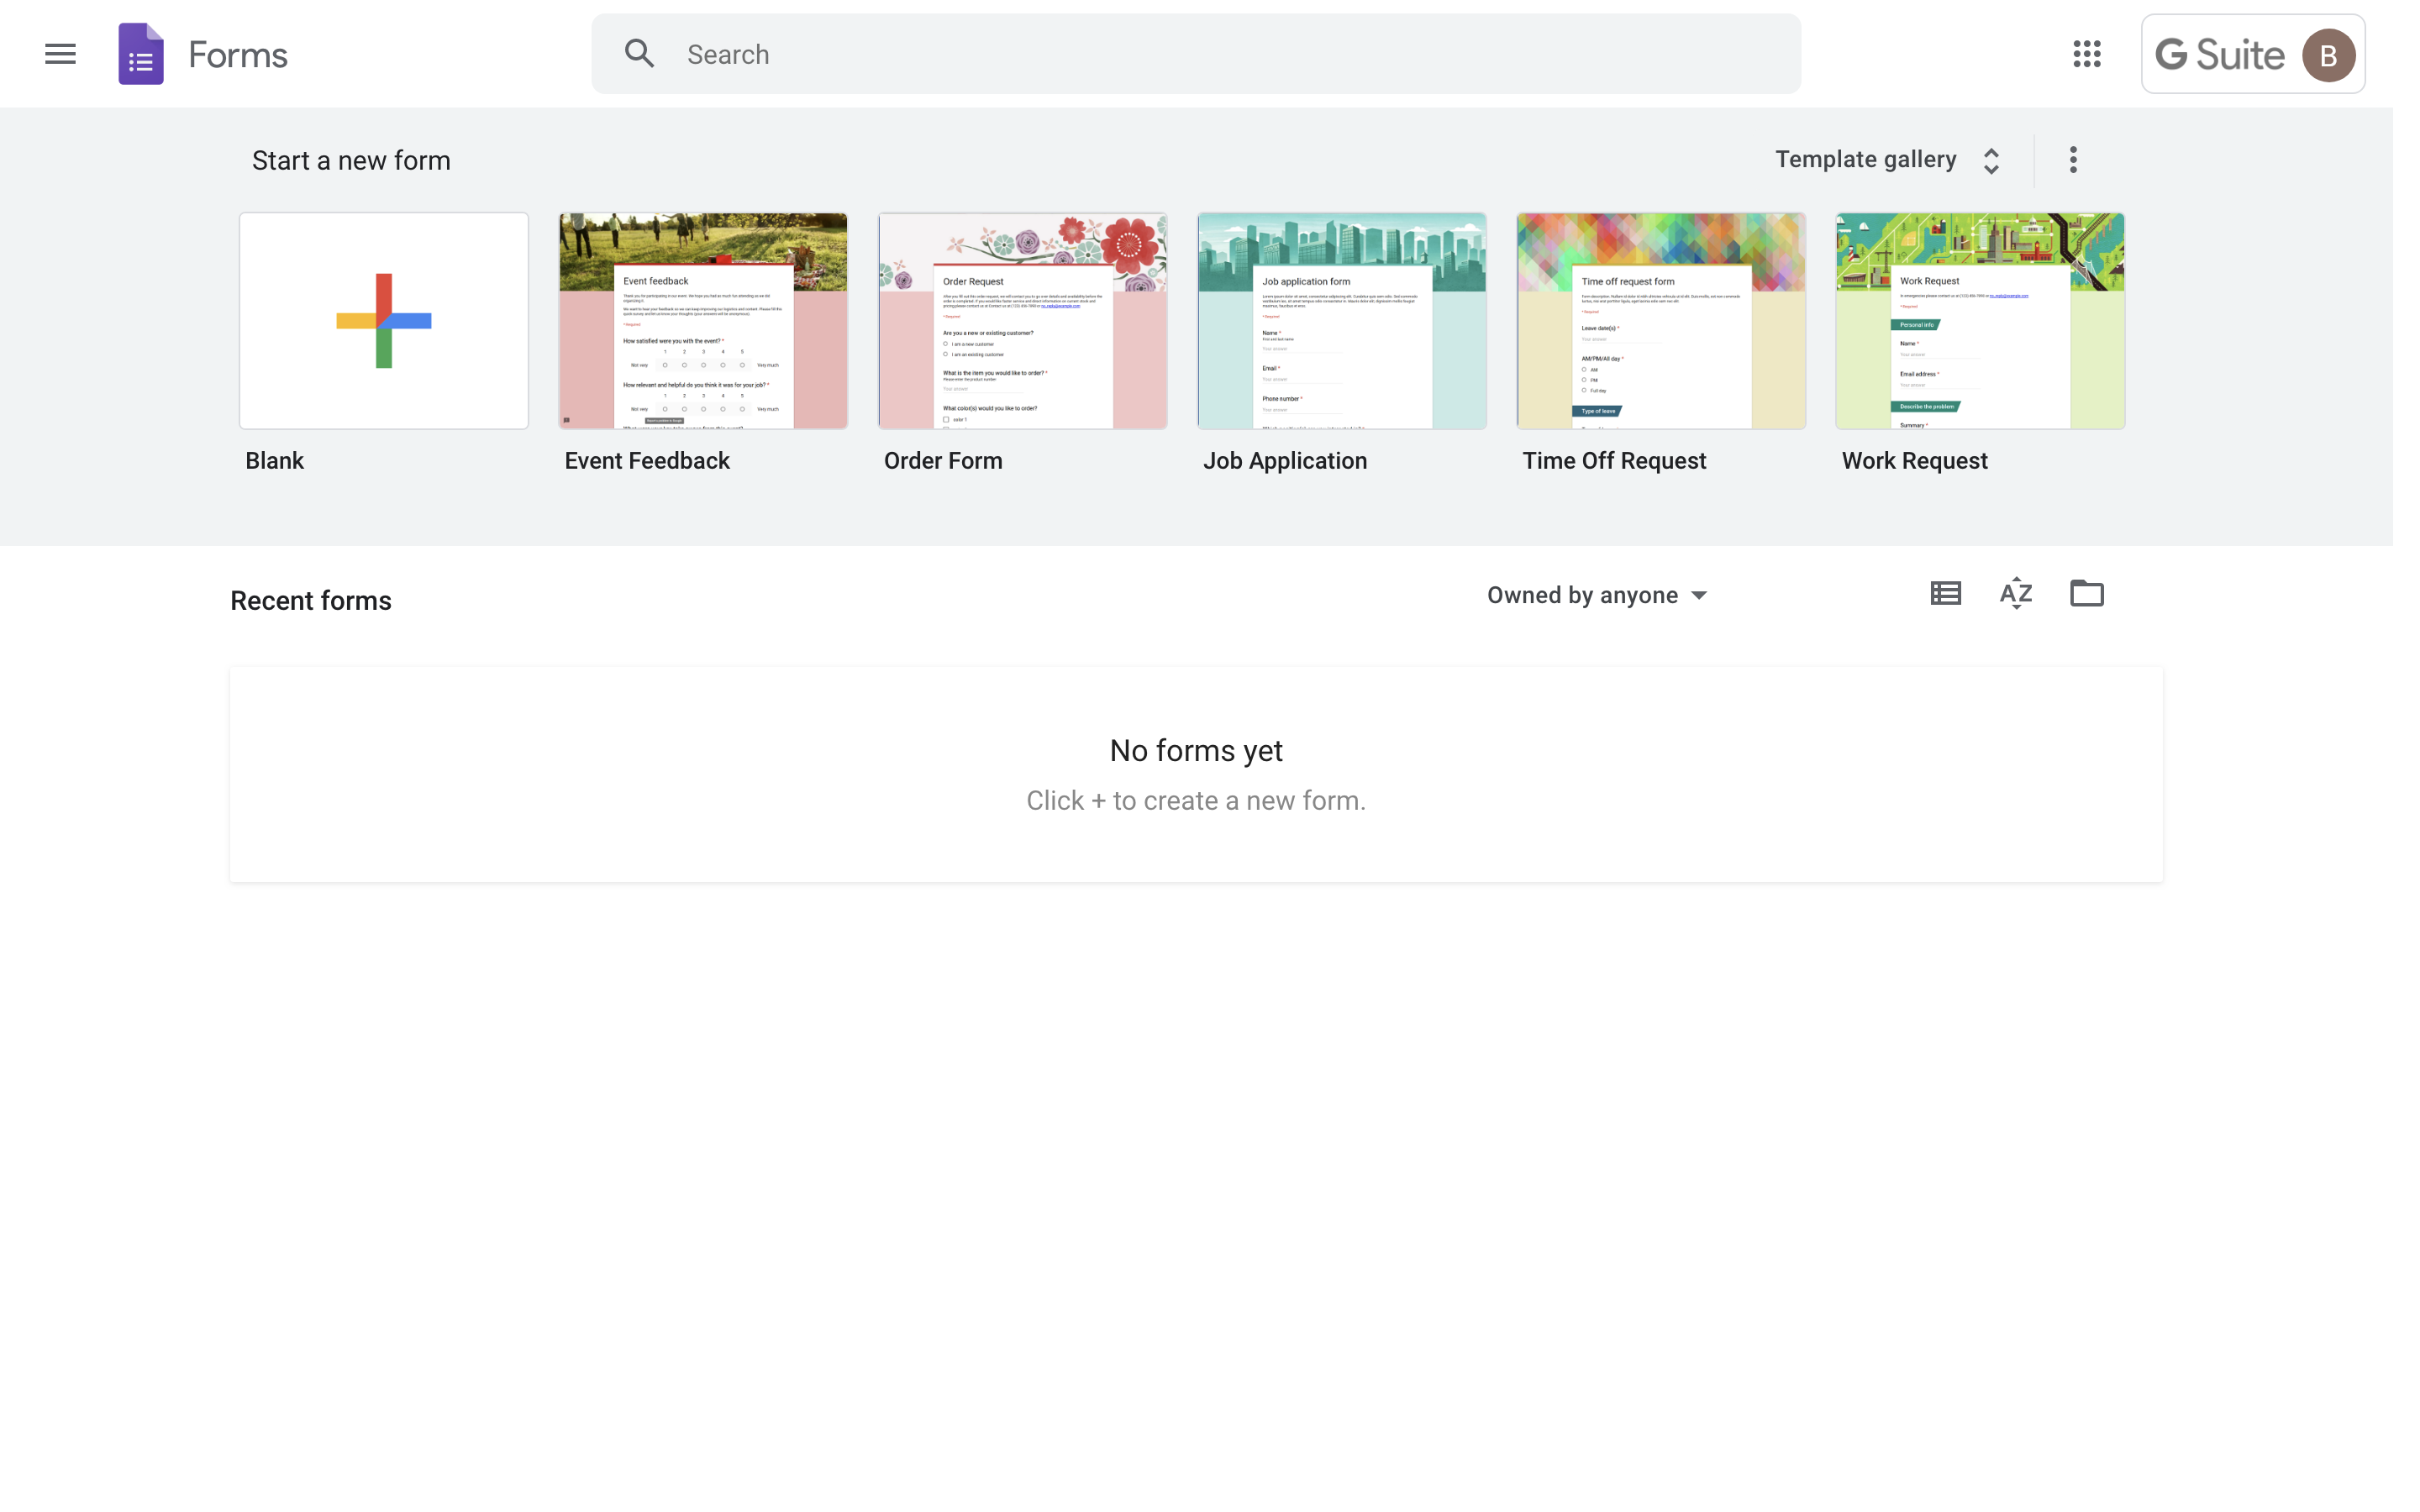
\includegraphics[width=1\textwidth]{img/gf/gf-dashboard}
		\caption{Google Form - Painel de Controlo}
		\label{fig:gf-dashboard}
	\end{center}
\end{figure}


\begin{figure}[ht!]
	\begin{center}
		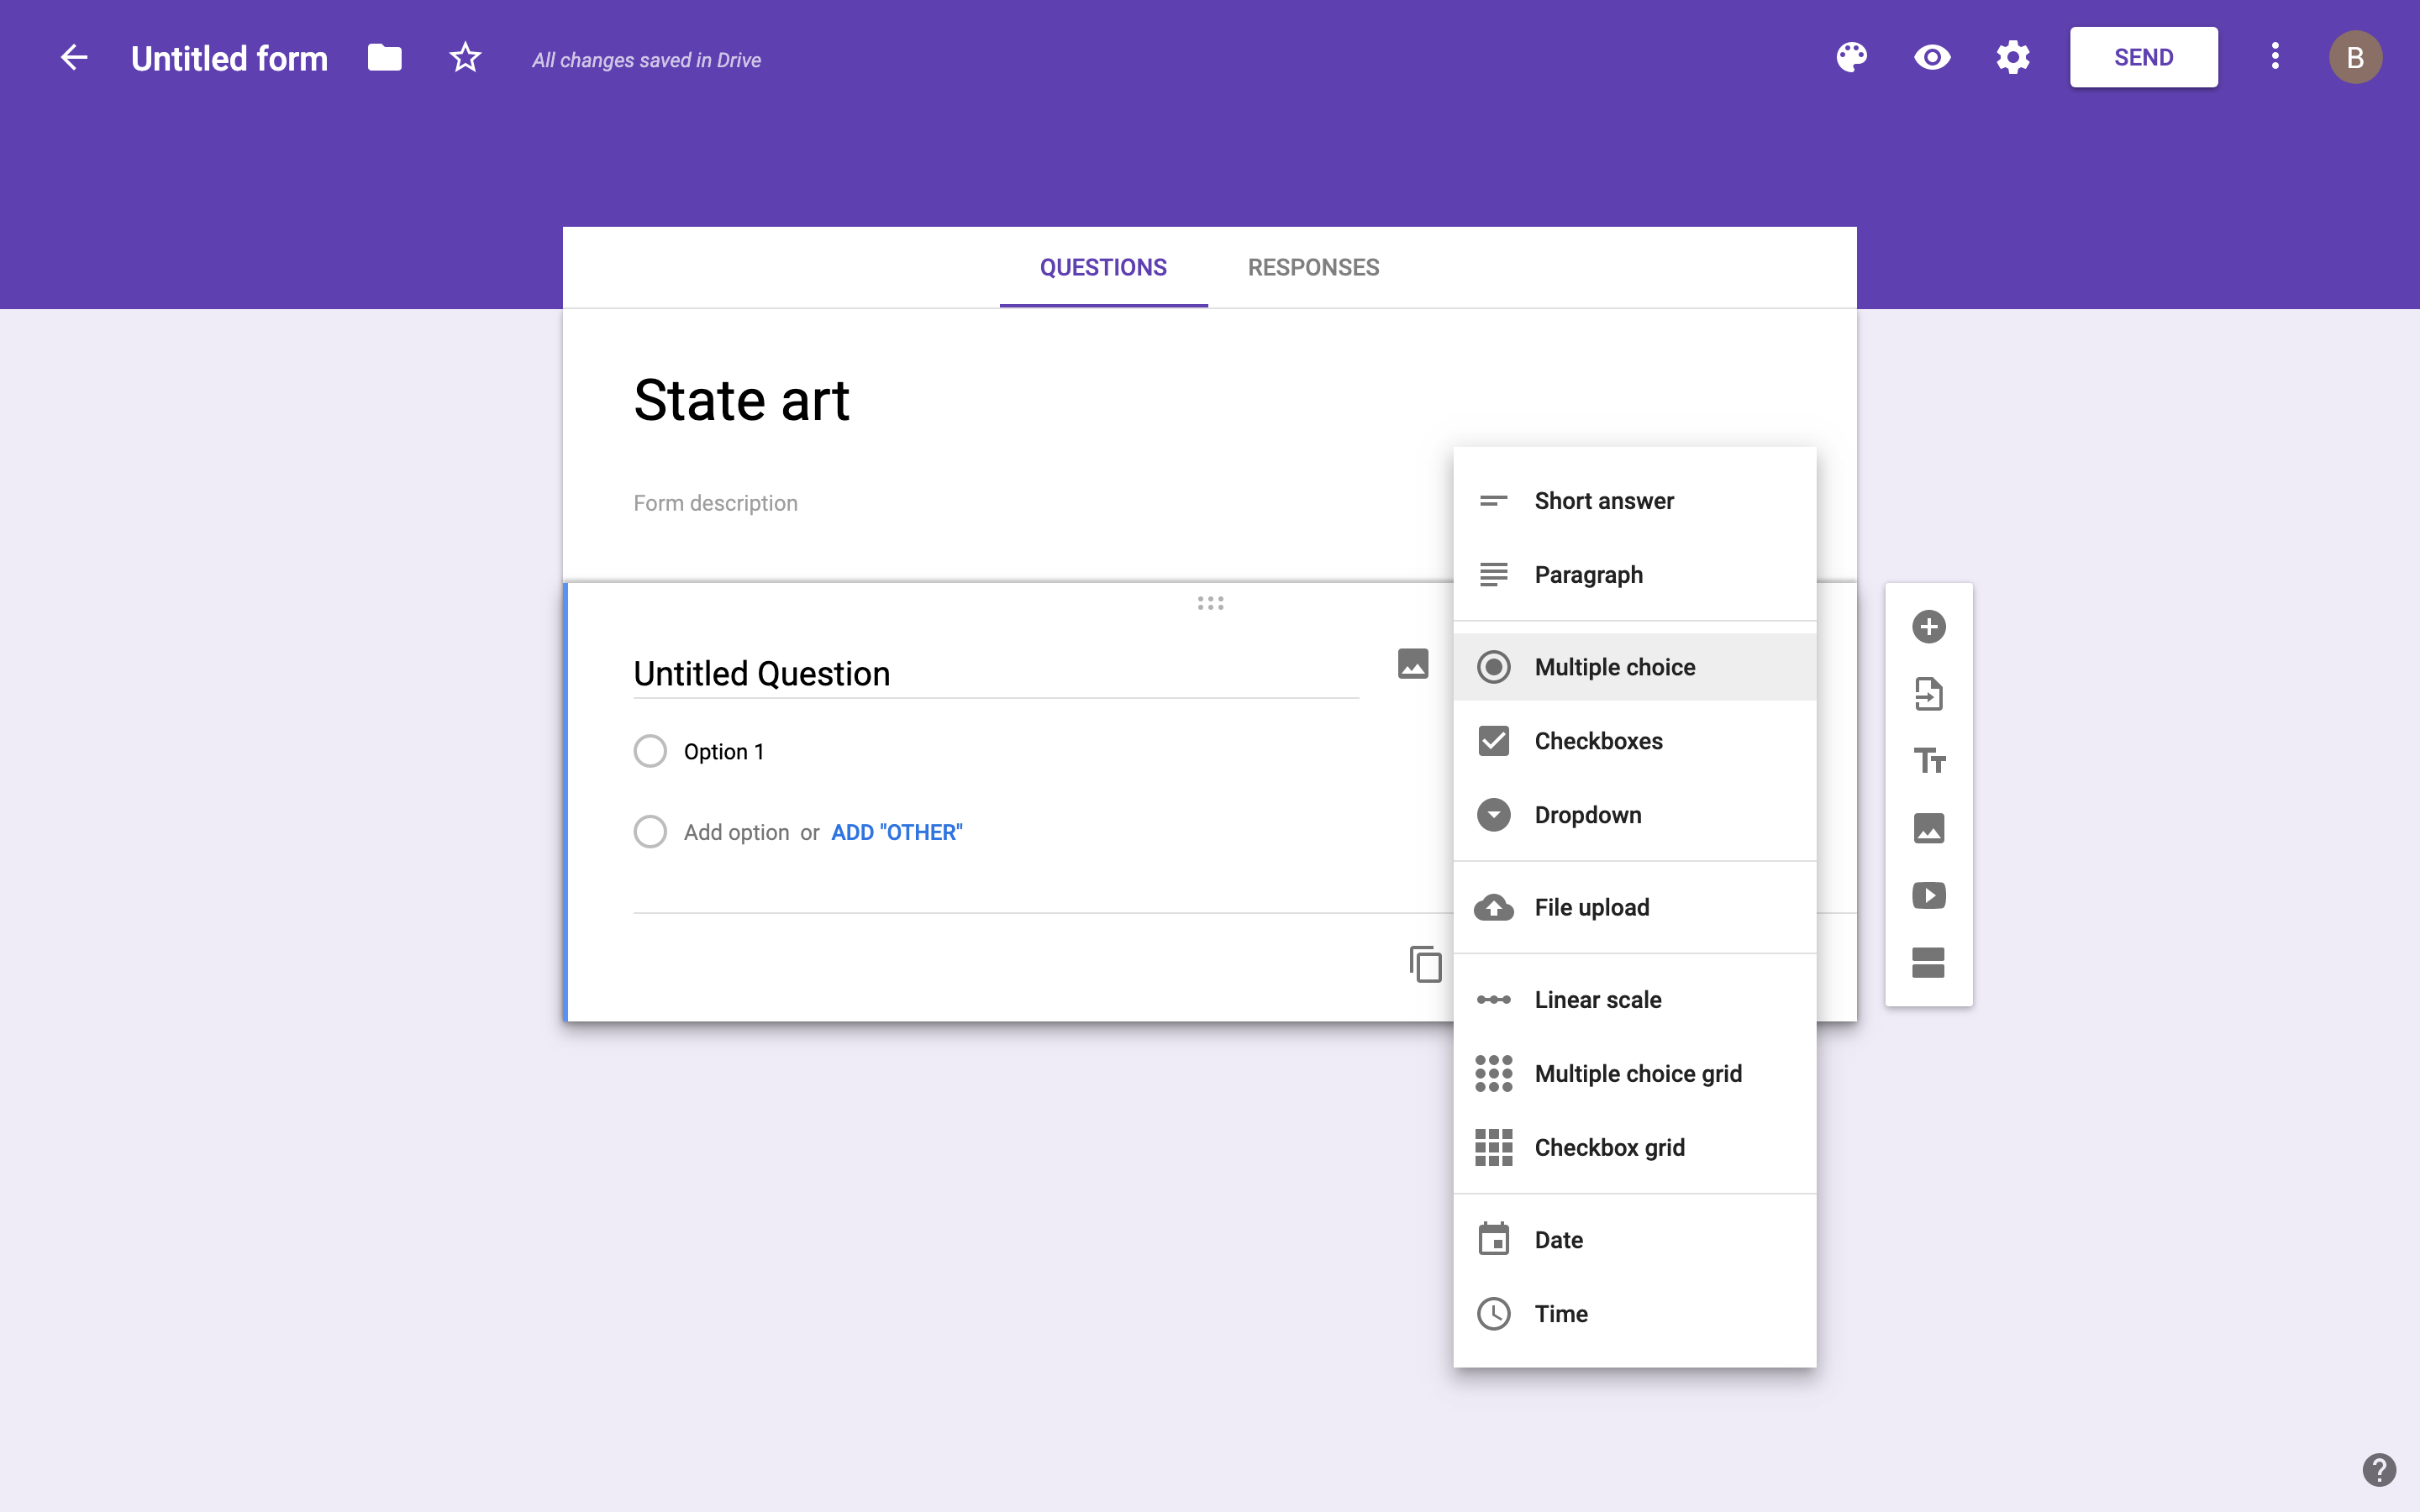
\includegraphics[width=1\textwidth]{img/gf/gf-form-q-type}
		\caption{Google Form - Tipos de perguntas}
		\label{fig:gf-form-q-type}
	\end{center}
\end{figure}

A Figura \ref{fig:gf-form-q-type} demonstra a criação de um formulário do zero. Há vários tipo de perguntas que a aplicação permite adicionar ao formulário e, apesar de se estar a criar um formulário novo, o google form permite importar um ou mais formulários diferentes, ao qual o utilizador tem acesso (i. e. formulários que estão disponíveis na sua área de trabalho), selecionando apenas as perguntas que deseja importar. Como podemos ver nas Figuras \ref{fig:gf-form-import}, \ref{fig:gf-form-import-select} e \ref{fig:gf-form-imported} as perguntas importadas foram colocadas na posição escolhida, que neste caso foi no final do formulário.

\begin{figure}[h!]
	\begin{center}
		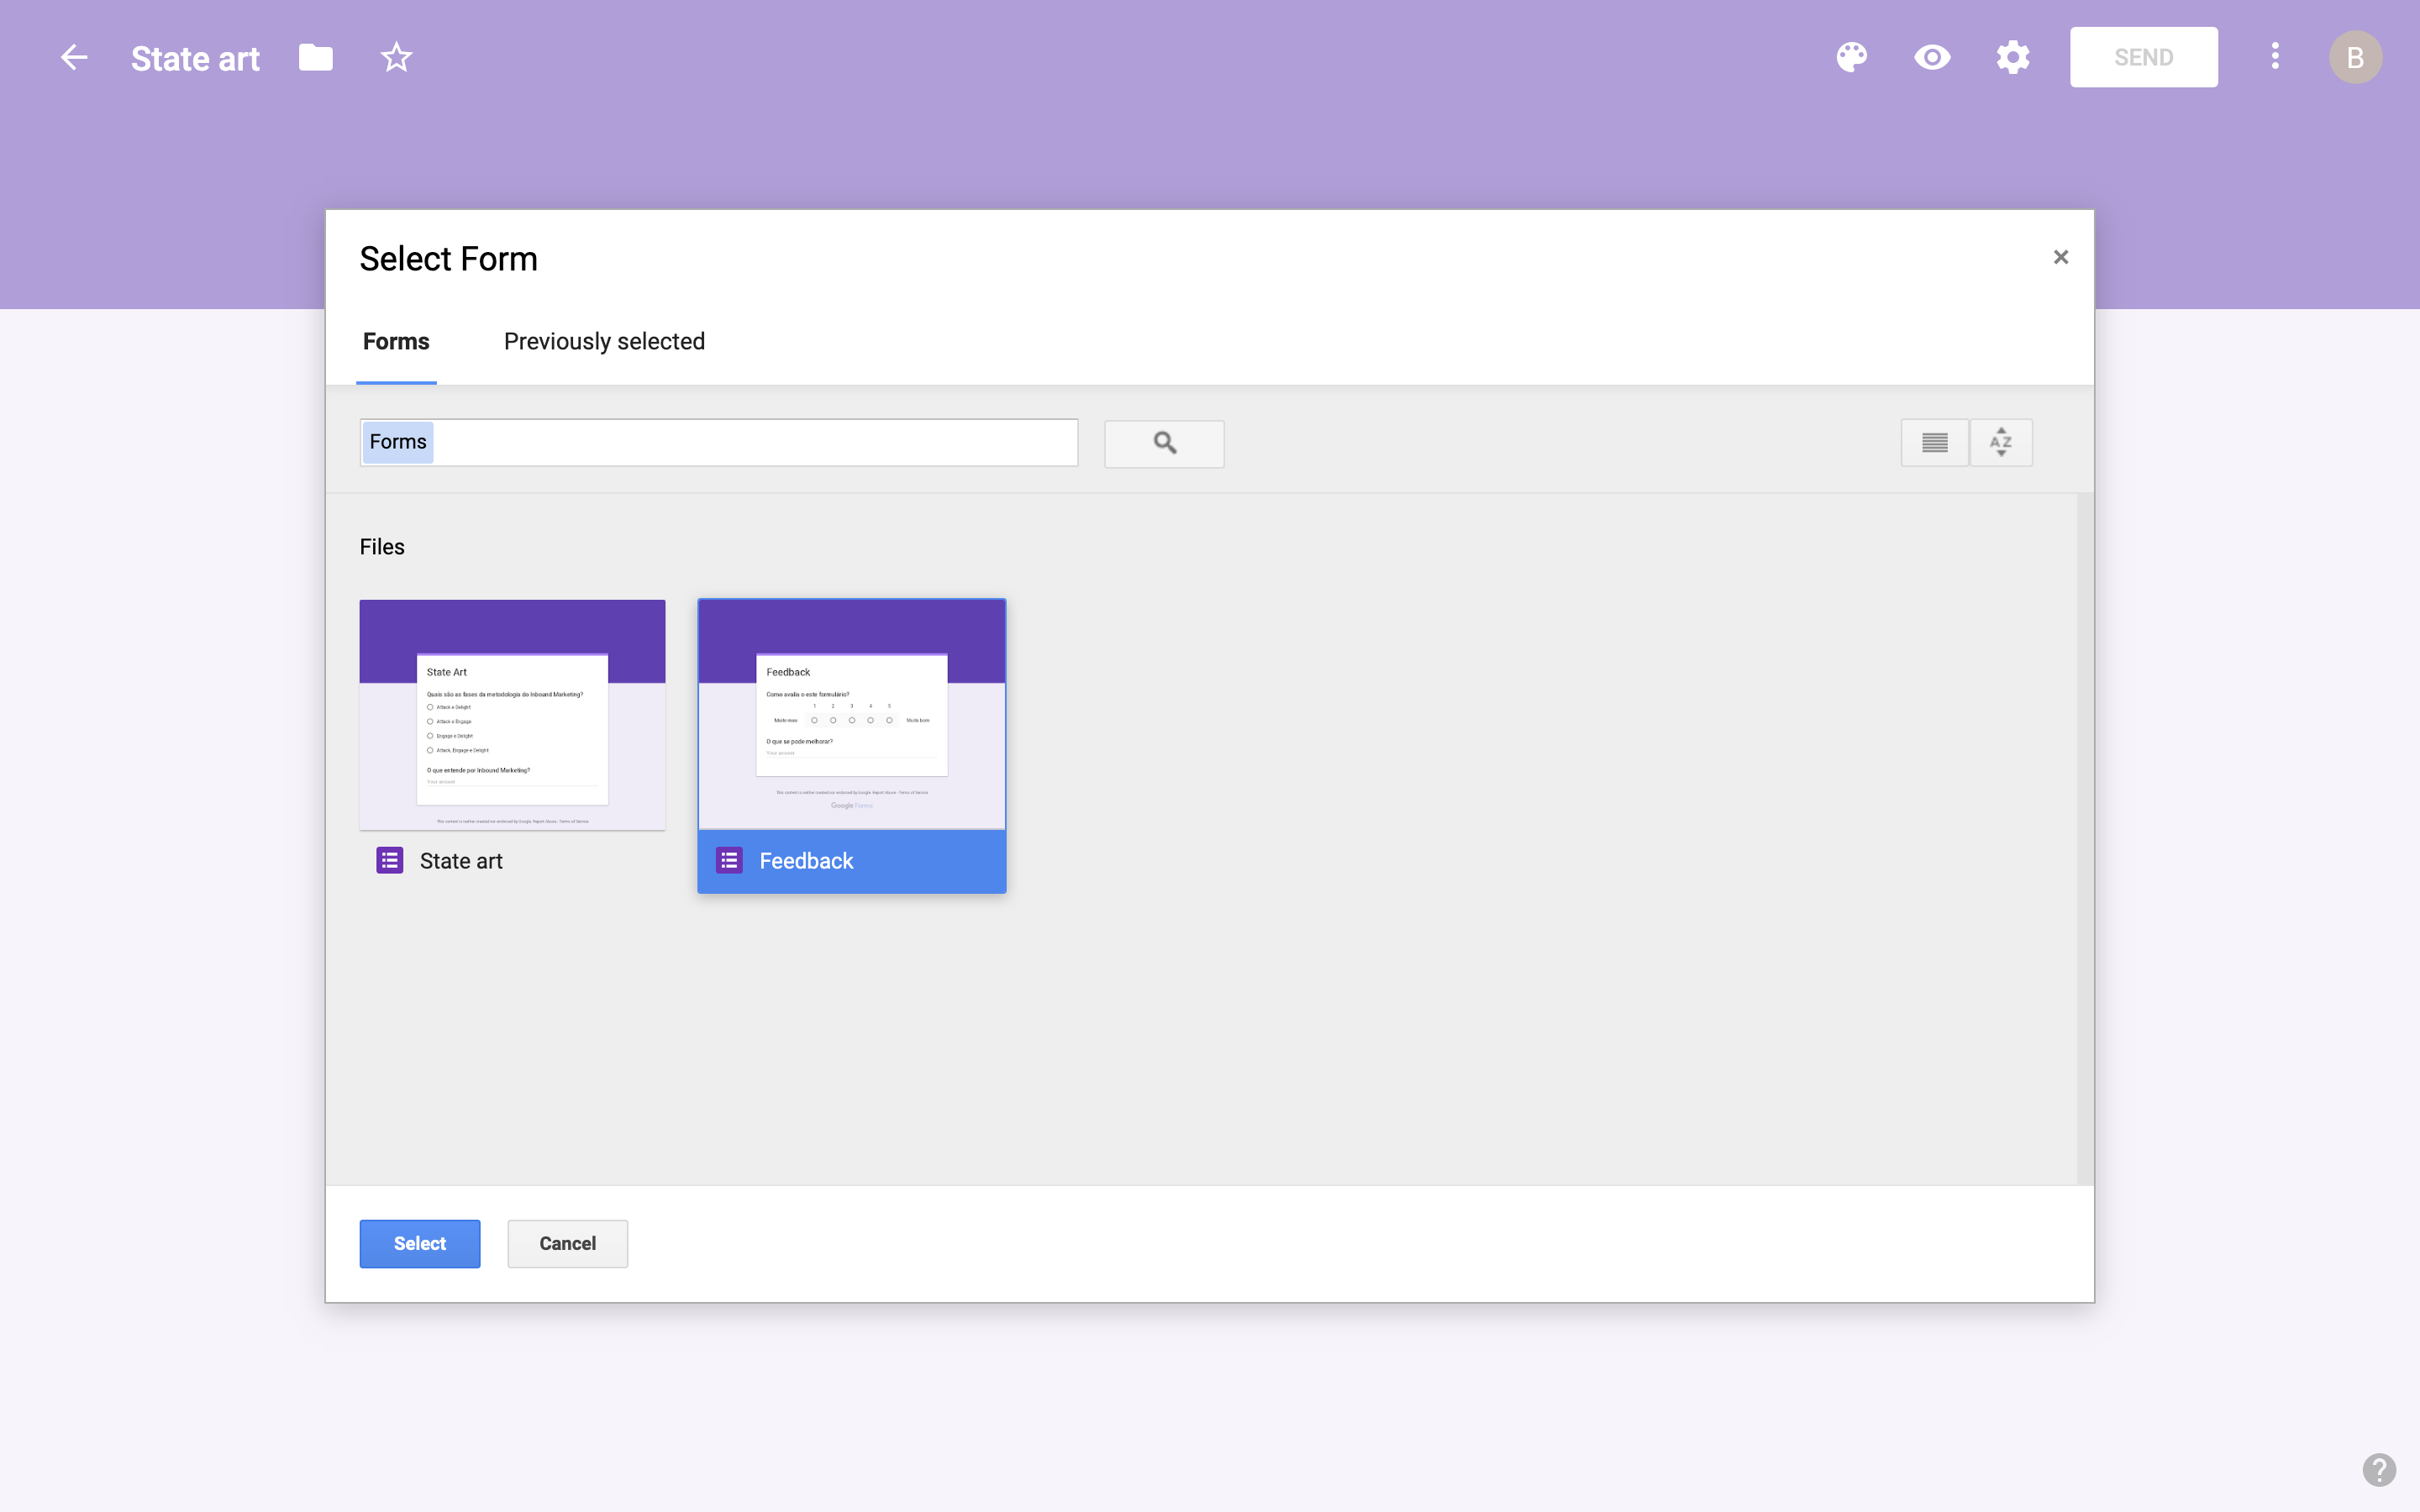
\includegraphics[width=1\textwidth]{img/gf/gf-form-import}
		\caption{Google Form - Importar formulário}
		\label{fig:gf-form-import}
	\end{center}
\end{figure}

\begin{figure}[h!]
	\begin{center}
		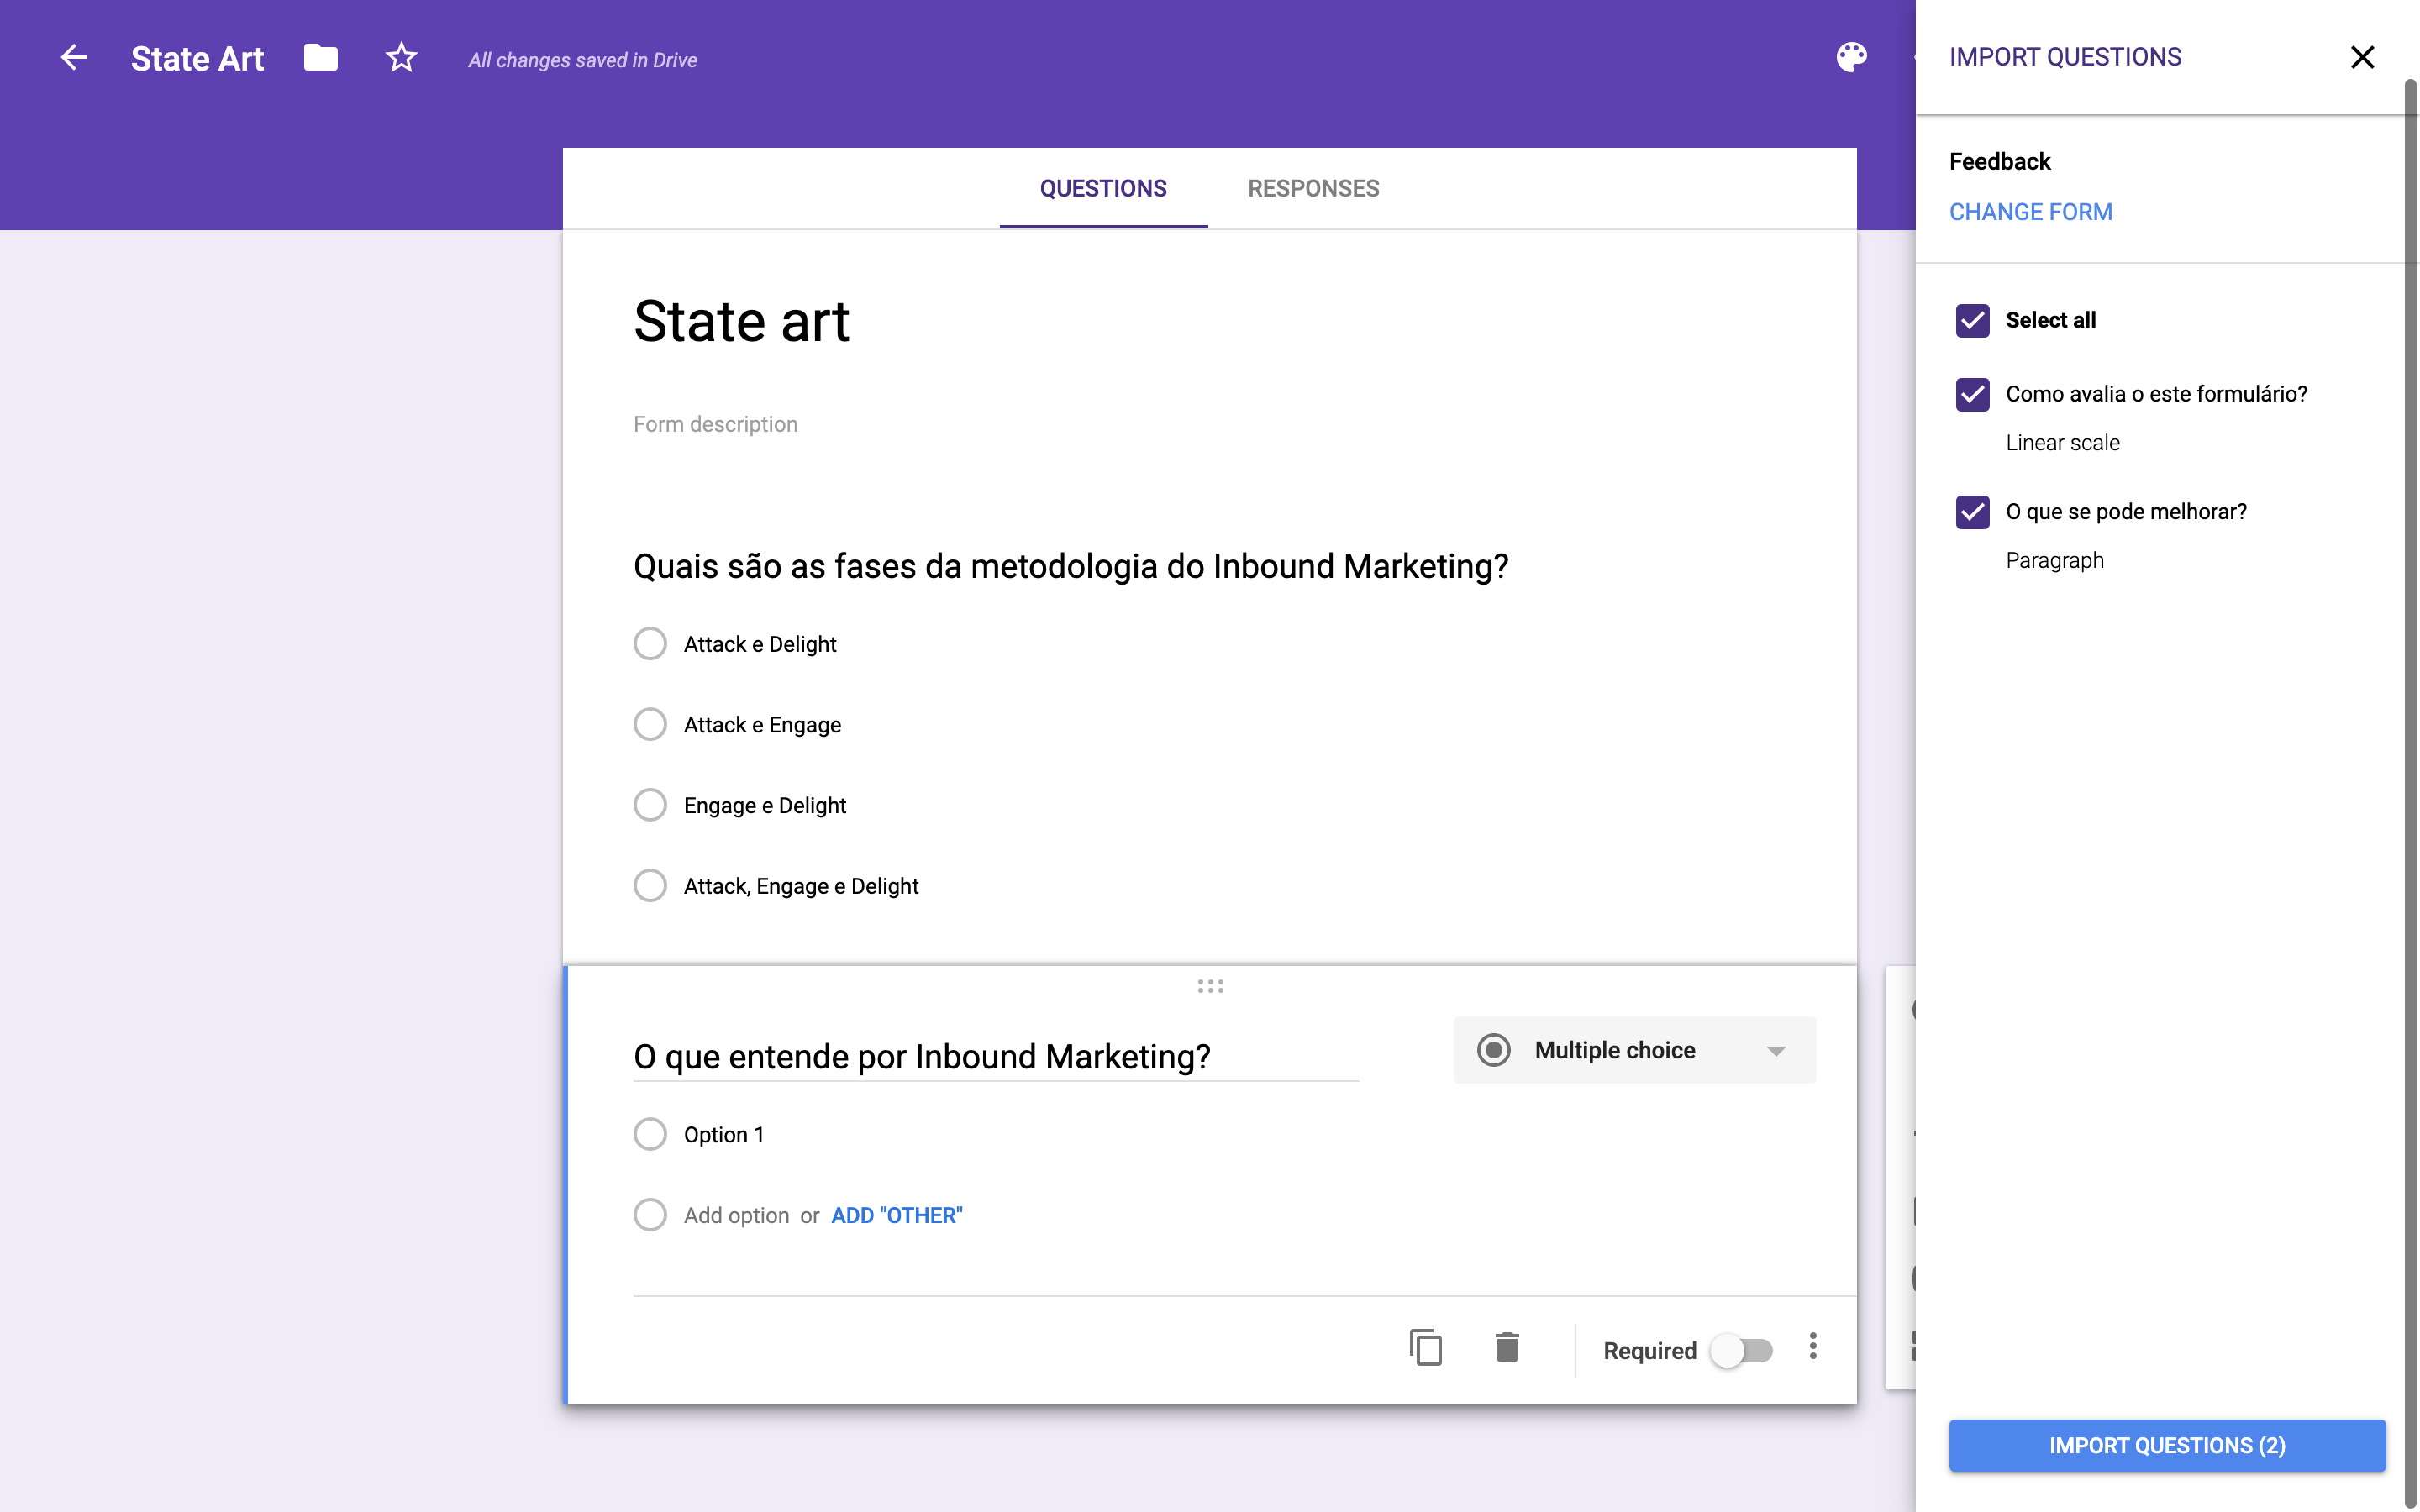
\includegraphics[width=1\textwidth]{img/gf/gf-form-import-select}
		\caption{Google Form - Selecionar perguntas a importar}
		\label{fig:gf-form-import-select}
	\end{center}
\end{figure}

\begin{figure}[h!]
	\begin{center}
		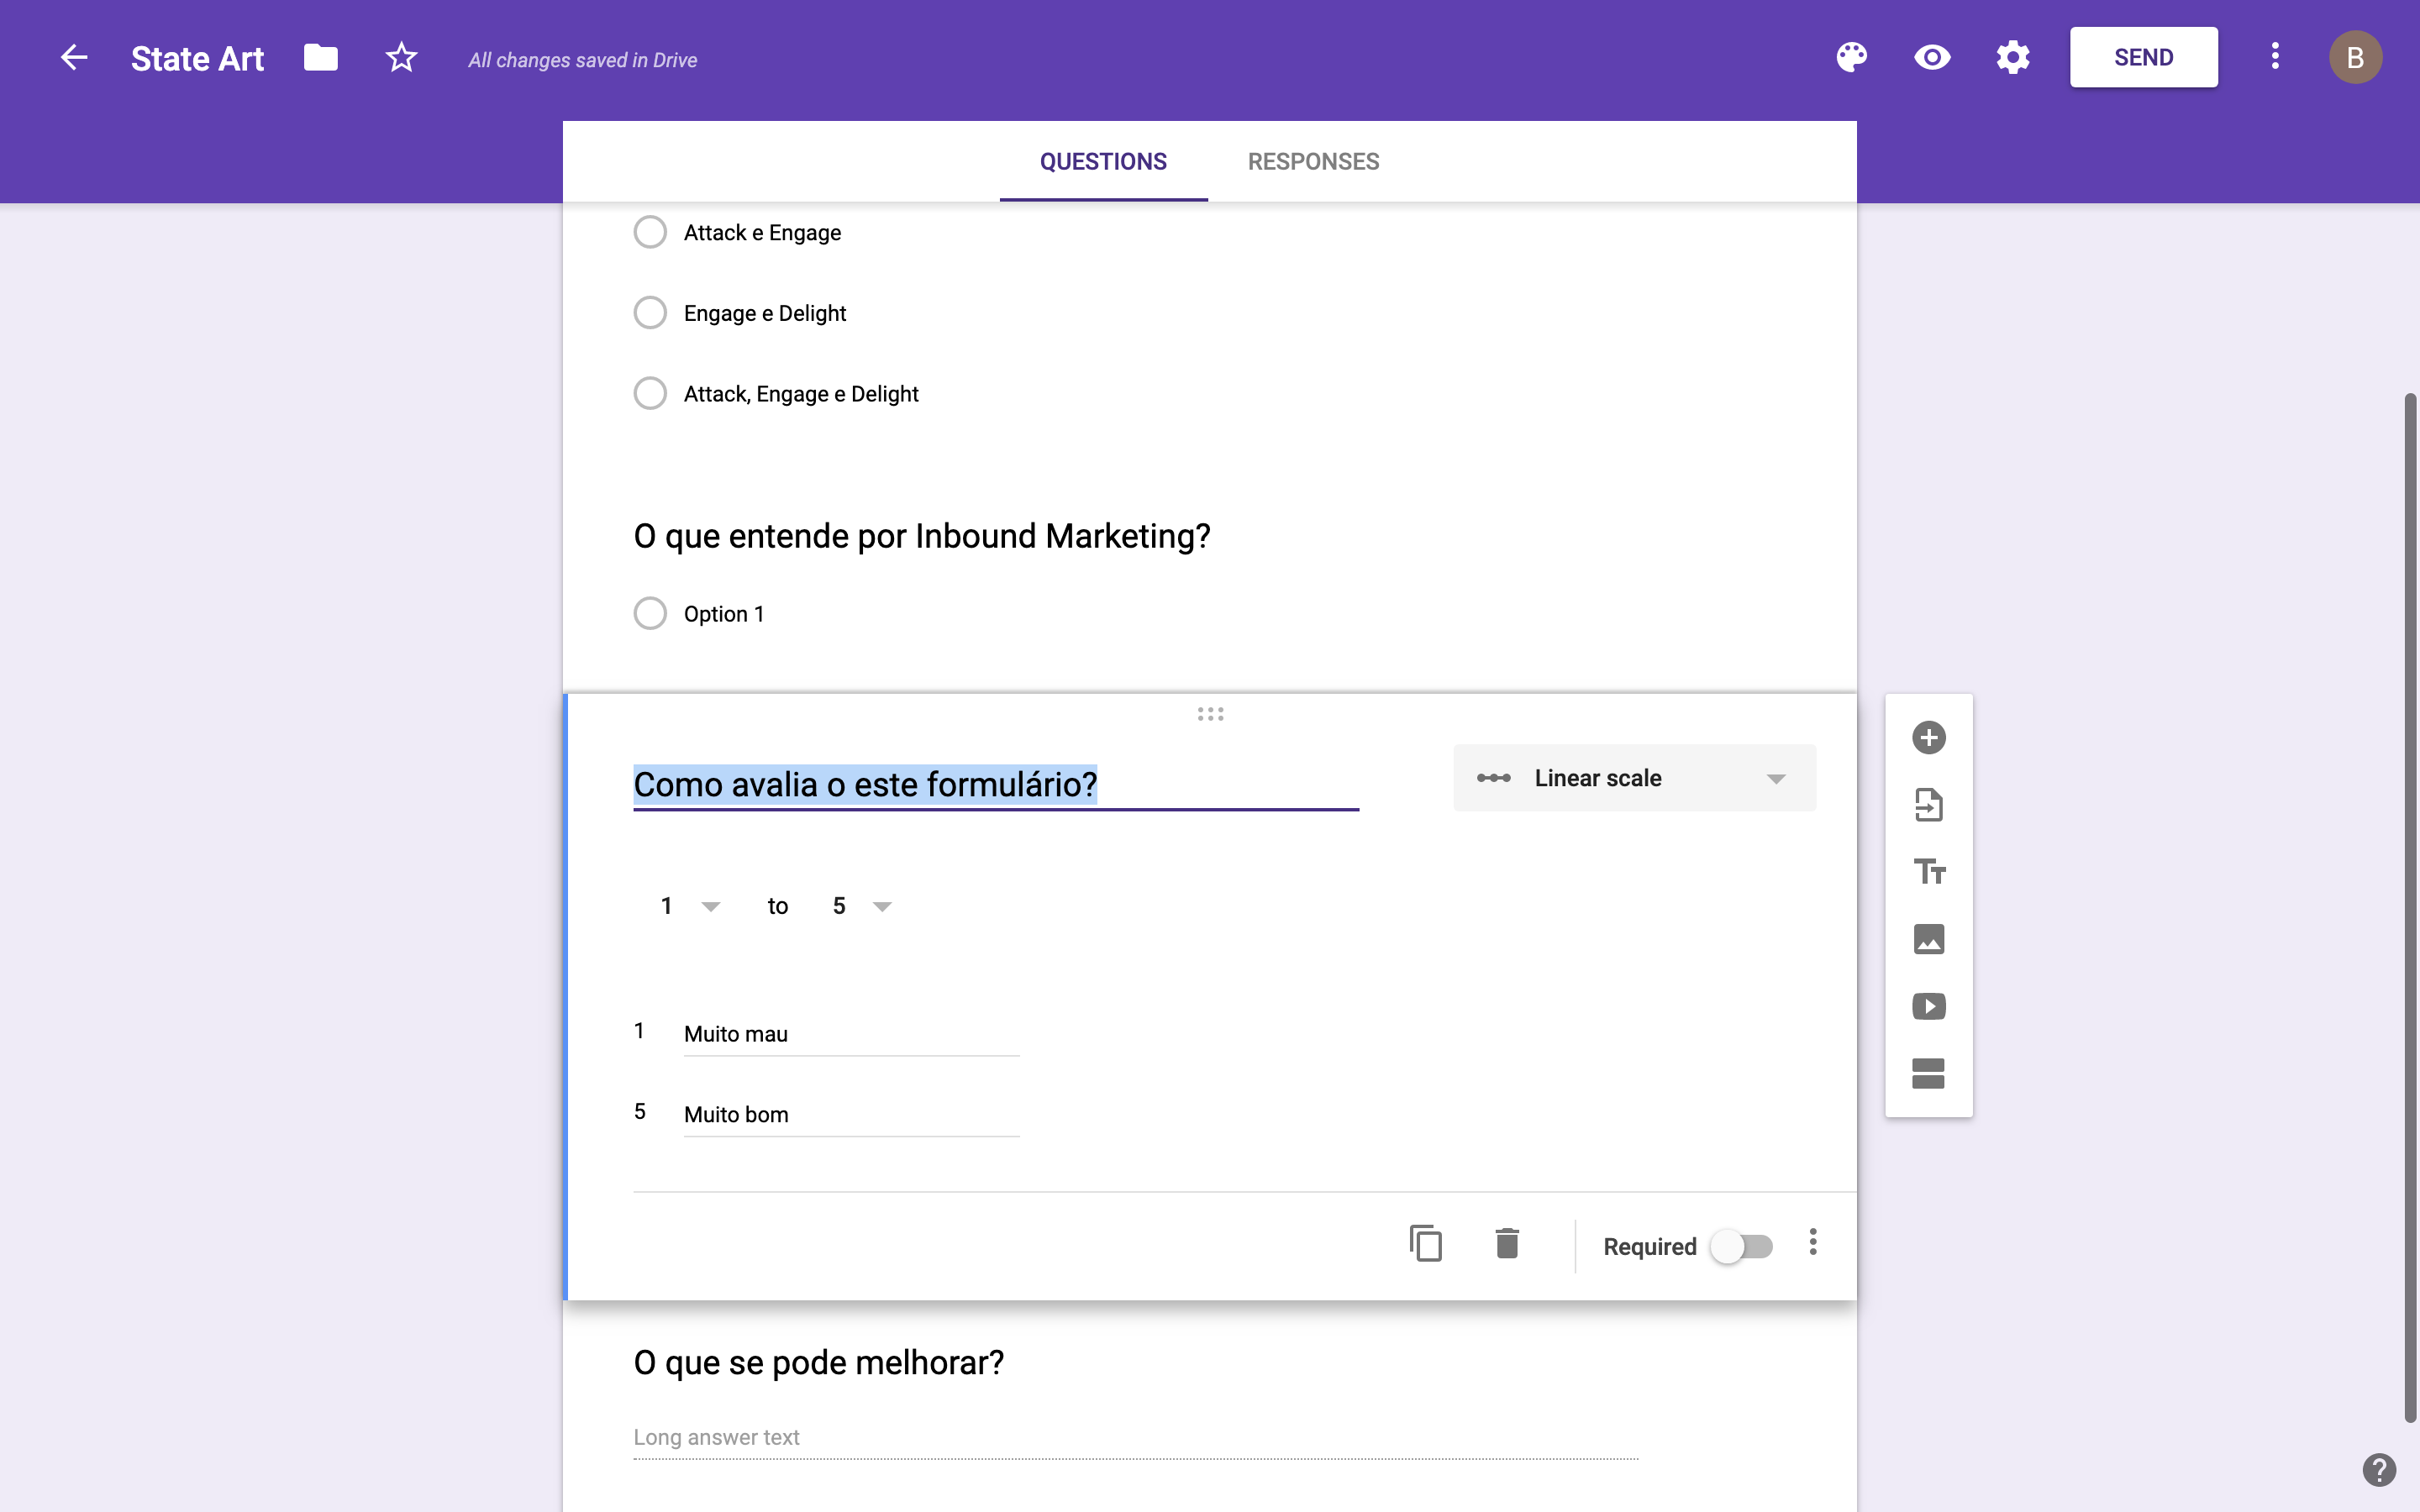
\includegraphics[width=1\textwidth]{img/gf/gf-form-imported}
		\caption{Google Form - Perguntas importadas}
		\label{fig:gf-form-imported}
	\end{center}
\end{figure}


\begin{figure}[h!]
	\begin{center}
		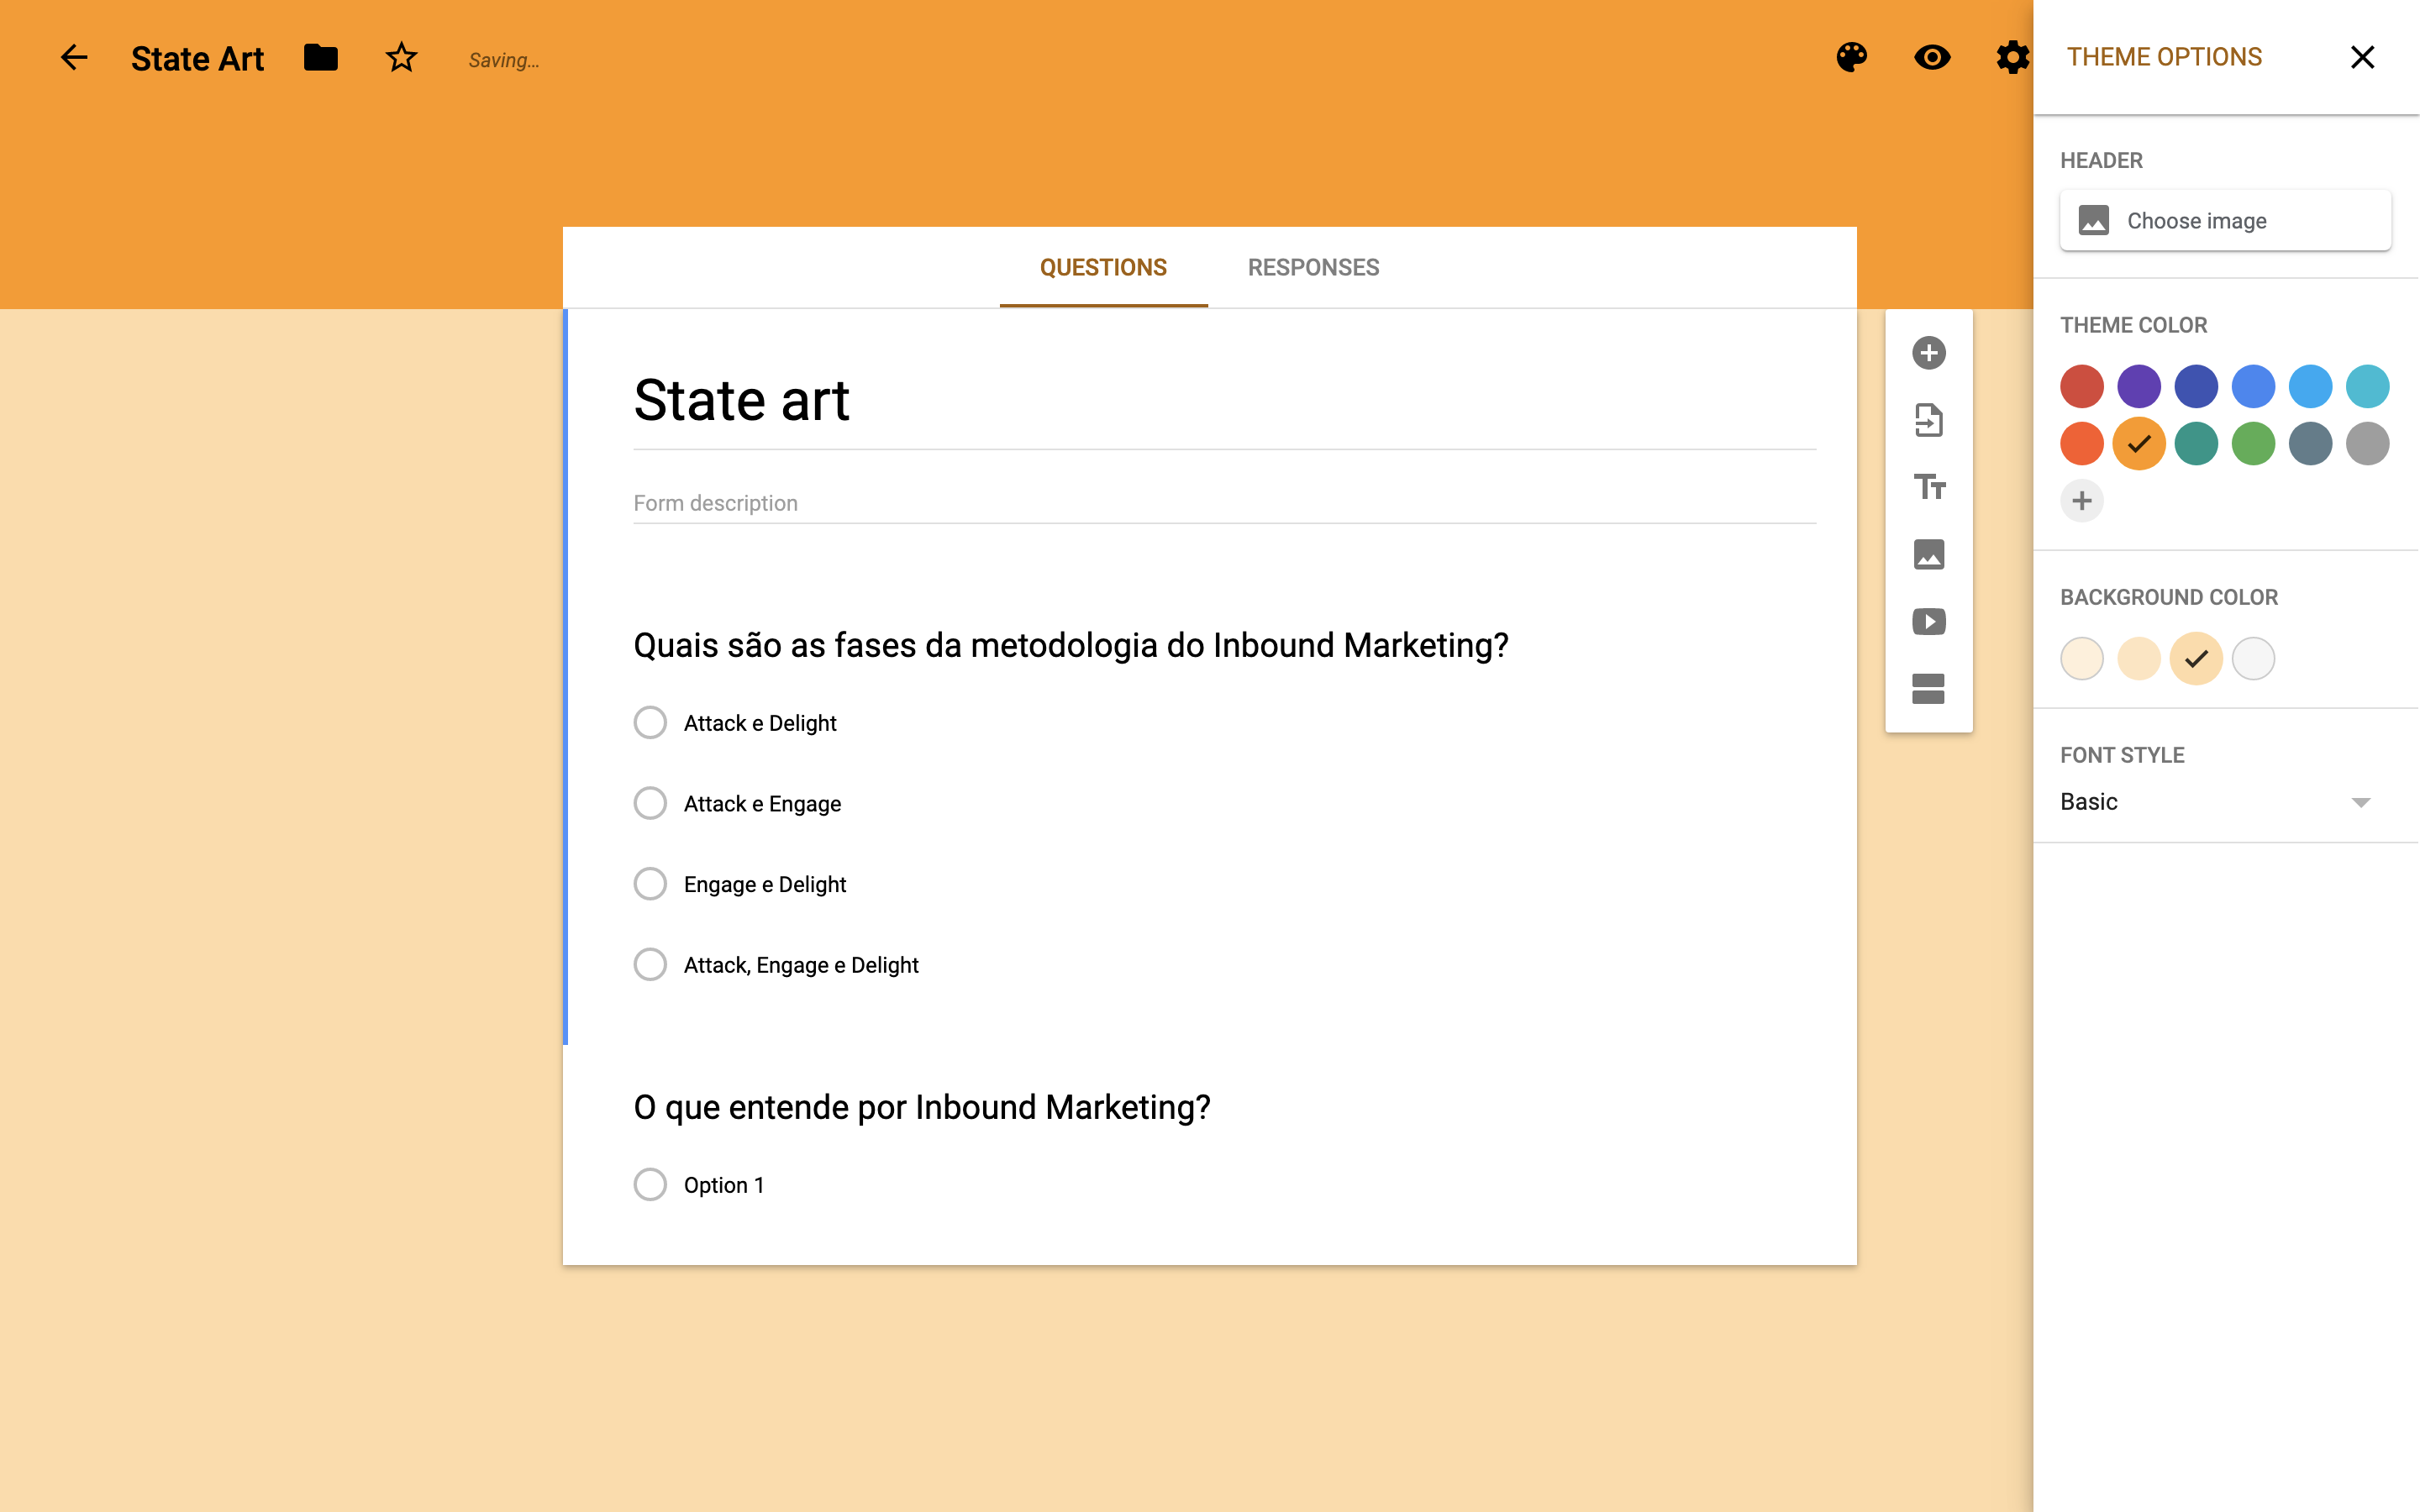
\includegraphics[width=1\textwidth]{img/gf/gf-form-design}
		\caption{Google Form - Alterar design do formulário}
		\label{fig:gf-form-design}
	\end{center}
\end{figure}

\newpage

Grande parte das plataformas e aplicações,no mercado, de criação de formulários permitem personalizar os formulários, ao gosto do utilizador, e o Google Form não é excepção. A aplicação permite alterar as definições padrão do formulário(Figuras \ref{fig:gf-form-set1}, \ref{fig:gf-form-set2} e \ref{fig:gf-form-set3}) e, apesar de se poder também personalidar o \textit{design} do formulário (\ref{fig:gf-form-design}), apens podemos alterar a cor ou imagem de fundo e fonte de texto.

\begin{figure}[ht!]
	\begin{center}
		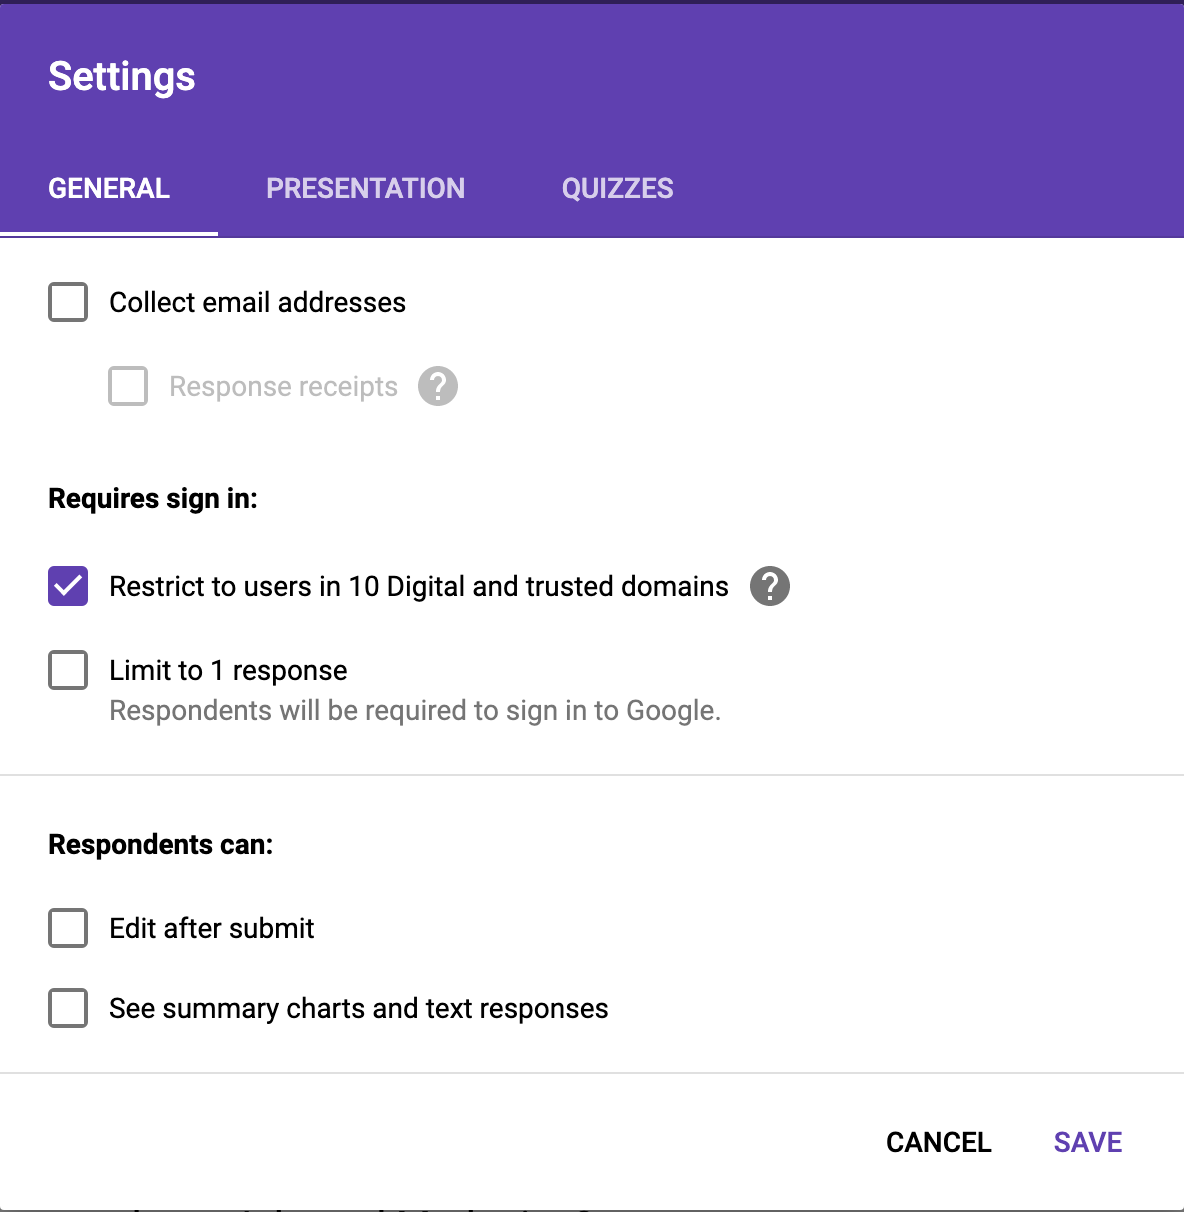
\includegraphics[height=.30\textheight]{img/gf/gf-form-set1}
		\caption{Google Form - Opções}
		\label{fig:gf-form-set1}
	\end{center}
\end{figure}

\begin{figure}[ht!]
	\begin{center}
		\begin{minipage}{0.40\textwidth}
			\begin{center}
				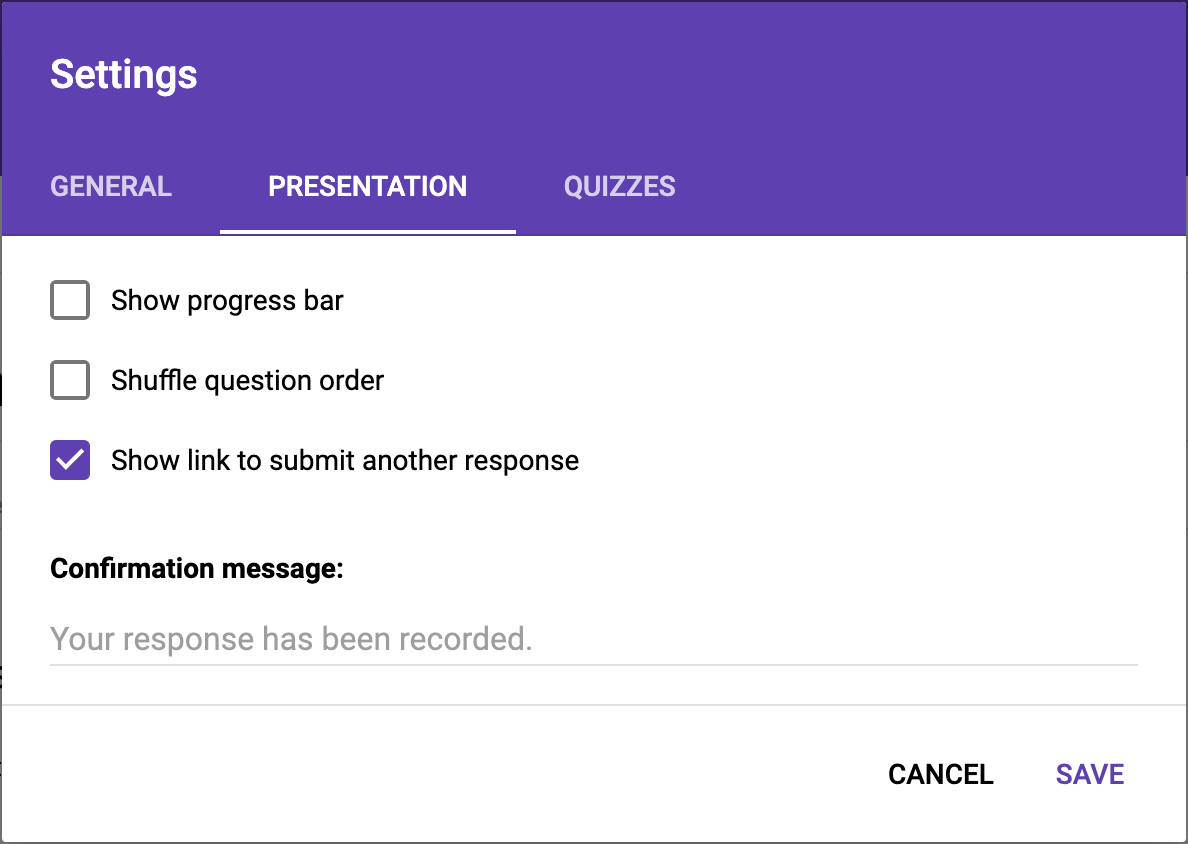
\includegraphics[height=.22\textheight]{img/gf/gf-form-set2}
				\caption{Google Form - Opções}
				\label{fig:gf-form-set2}
			\end{center}
		\end{minipage}
		\hspace{2cm}
		\begin{minipage}{0.40\textwidth}
			\begin{center}
				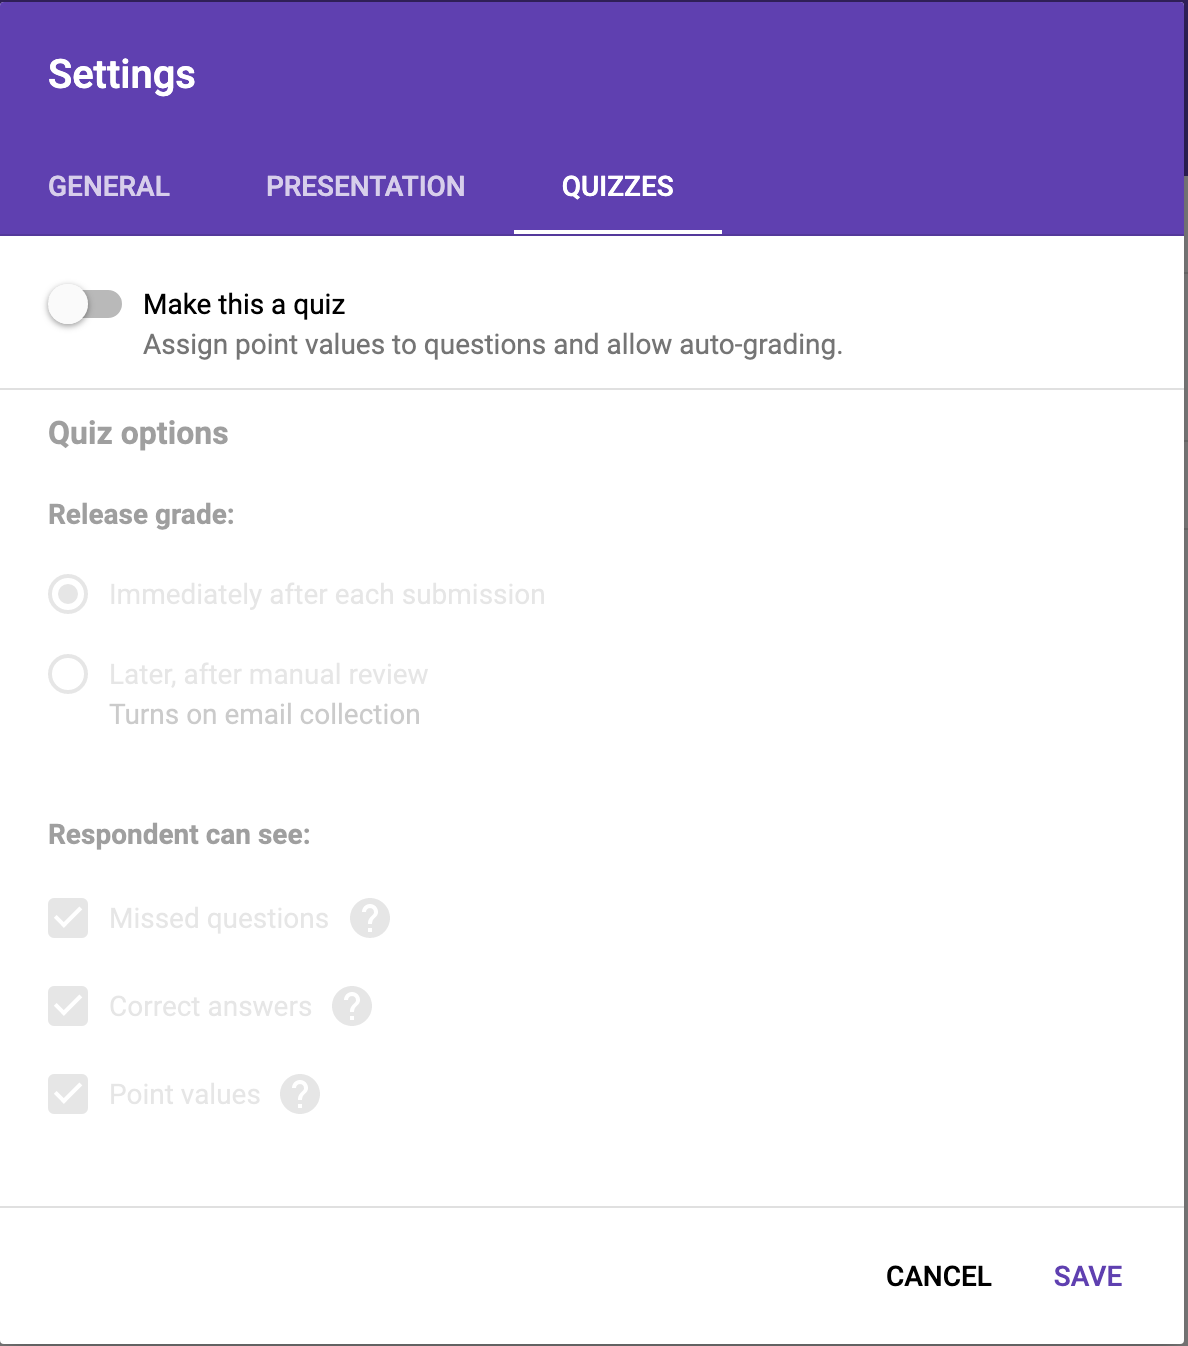
\includegraphics[height=.30\textheight]{img/gf/gf-form-set3}
				\caption{Google Form - Opções}
				\label{fig:gf-form-set3}
			\end{center}
		\end{minipage}
	\end{center}
\end{figure}

Antes de partilhar o formulário, precisamos de verificar se o formulário ficou construido como planeado e para isso a aplicação fornece a funcionalidade: \textit{preview}. O Google Form permite os utilizadores enviarem o formulário através de um link, por email, embebido num pagina web ou partilhando no Facebook ou Tweeter utilizando os botões de partilha rápida.

Na análise de resultados, como podemos ver na Figura \ref{fig:gf-form-results} a aplicação faz uma exibição do resumo das respotas, mostrando alguns gráficos/estatisticas contudo, o utilizador não dispõe de nenhuma funcionalidade que filtra ou segmenta os dados. A unica maneira que o utilizador tem de poder tratar os dados e segmenta-los é, depois de exportar os dados, utilizando o Google Sheets, que já requer algum conhecimento na ferramenta. 

\newpage
\mbox{}

\begin{figure}[ht!]
	\begin{center}
		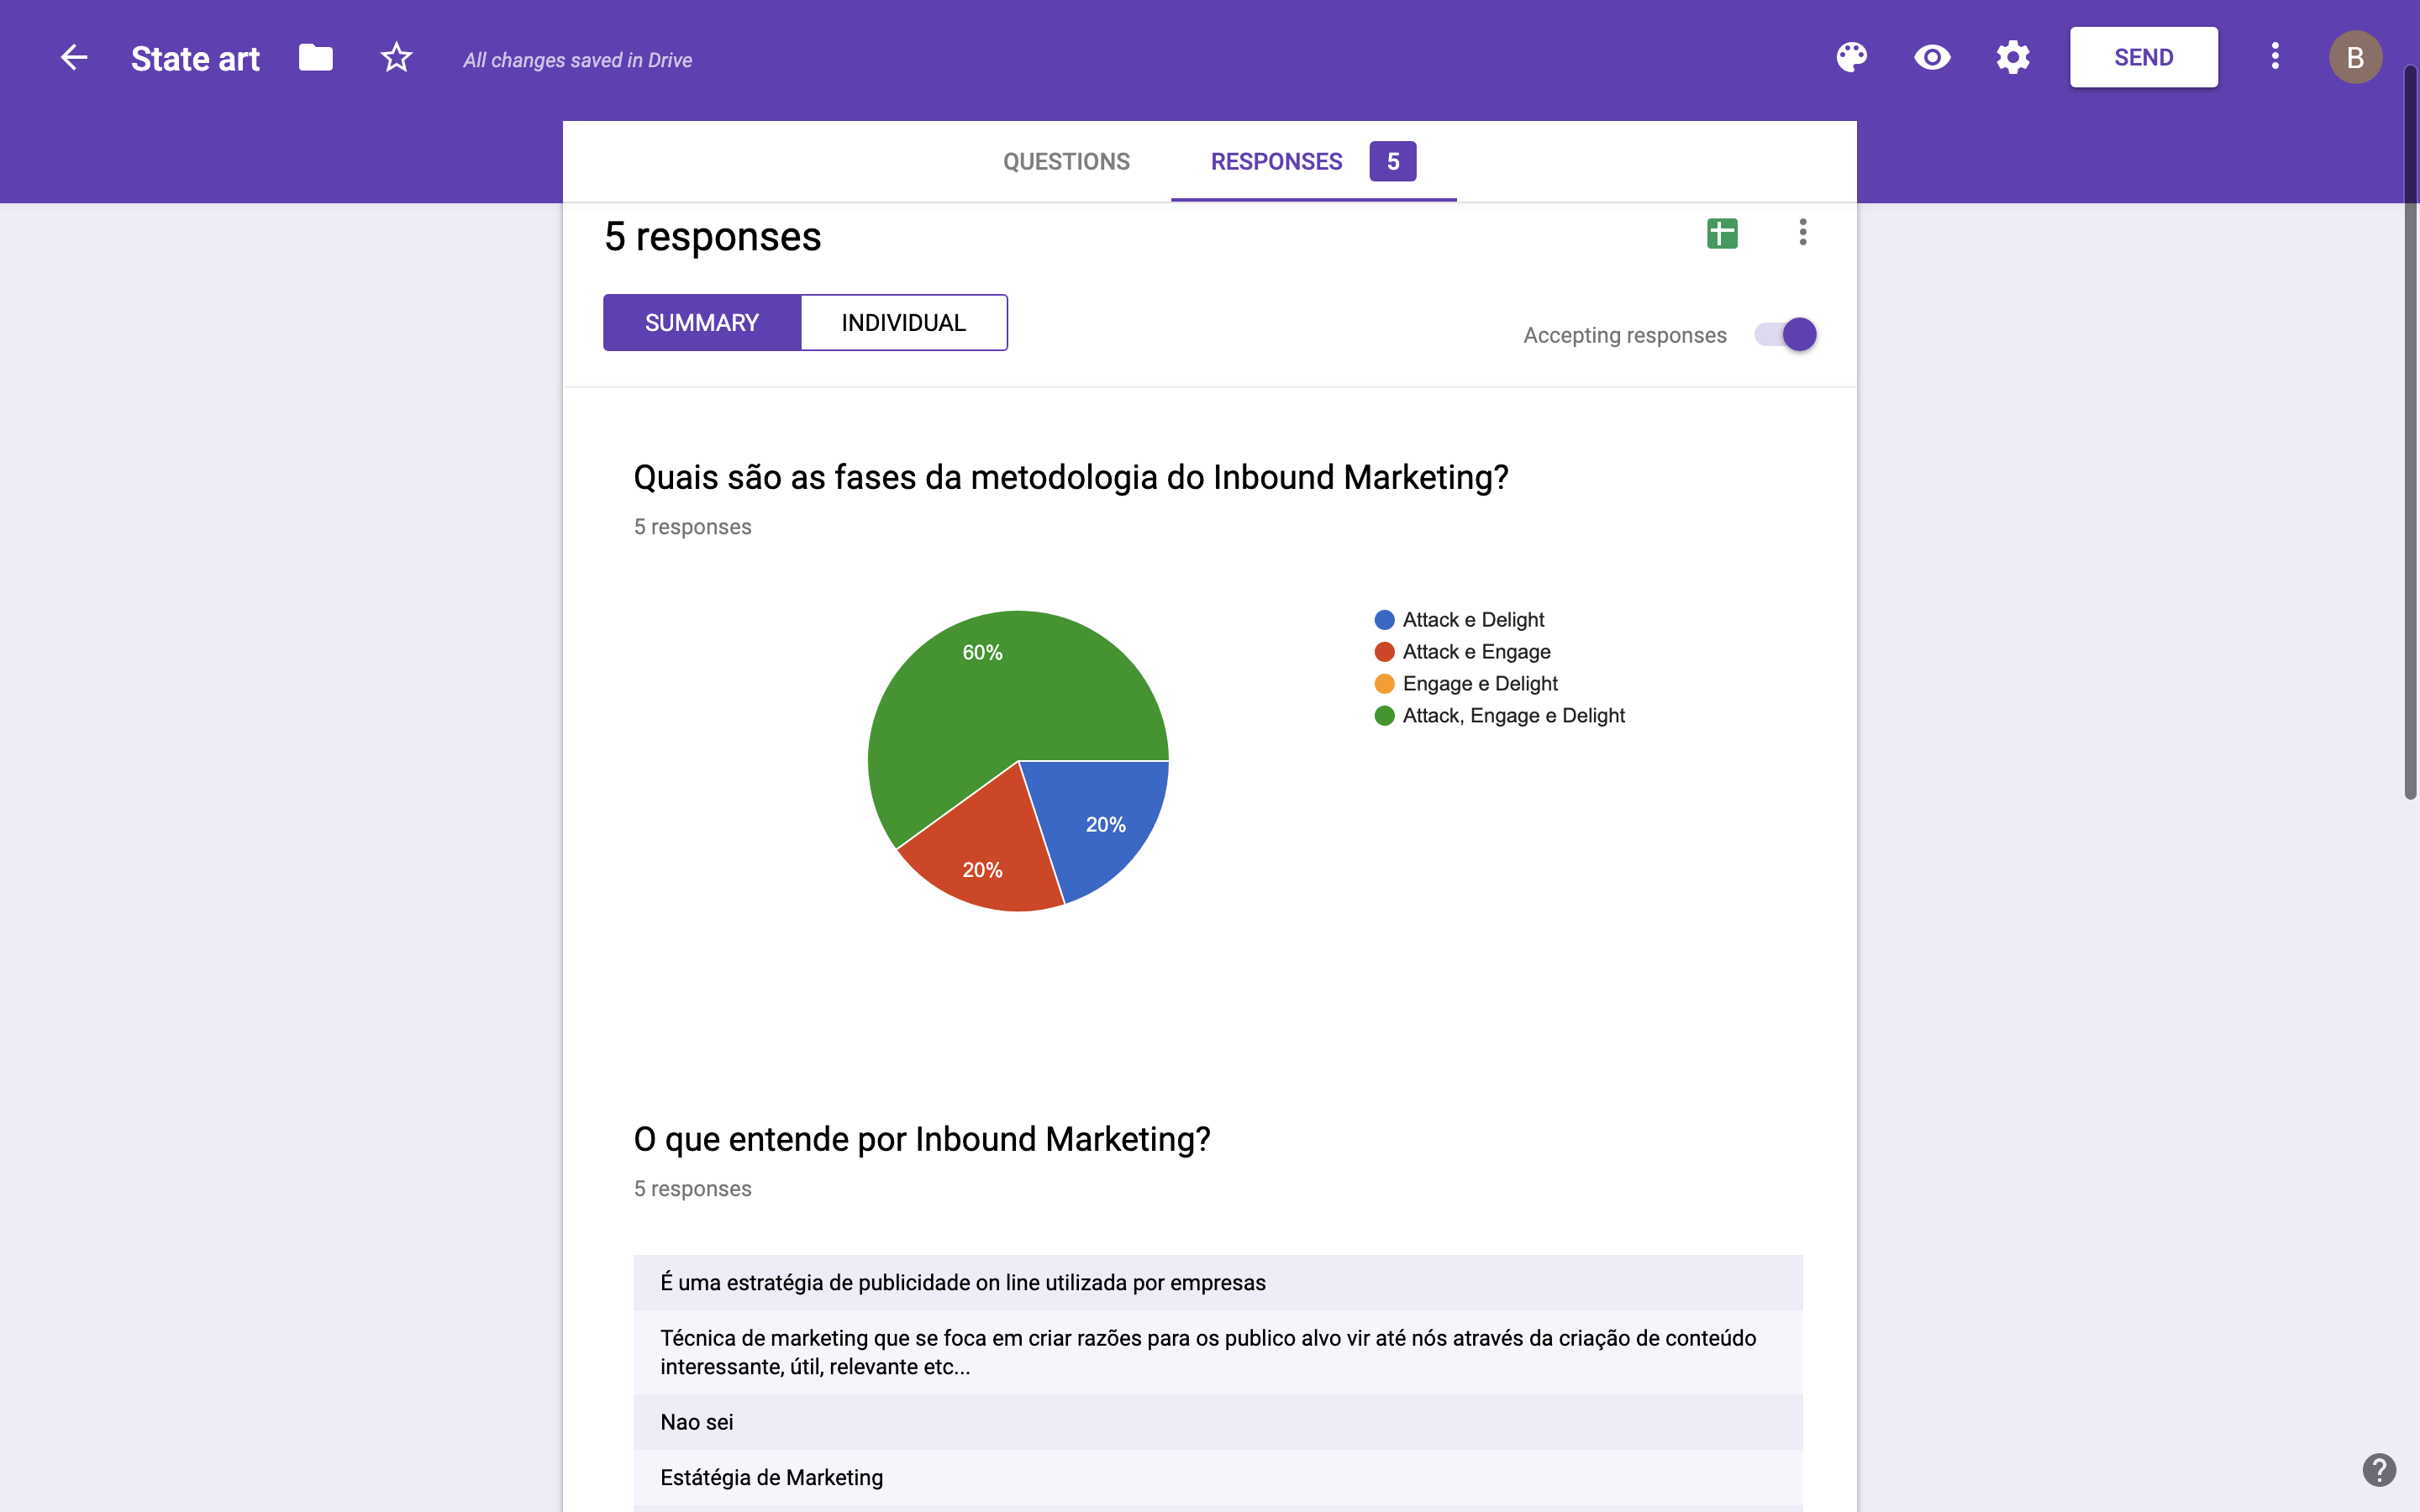
\includegraphics[width=1\textwidth]{img/gf/gf-form-results}
		\caption{Google Form - Sumério dos resultados obtidos}
		\label{fig:gf-form-results}
	\end{center}
\end{figure}

\section{\acrfull{tcg}}
\label{sec:TCG}

O \acrlong{tcg} é um produto actualmente no mercado, desenvolvido pela equipa da 10.digital, que tem como principal objectivo transformar PDFs numa aprendizagem baseada em tentativa erro. O \acrshort{tcg} nasceu de uma forte convicção de que perder apenas 2 minutos por dia numa formação tentativa erro é uma optima forma de aprender, poupando tempo e dinheiro às empresas. Inicialmente muito focado em formação interna, a equipa do \acrshort{tcg} foi-se apercebendo que existem muitos outros problemas (e. g. Consolidação de procedimentos, \textit{Onboarding} de novos colaboradores, Divulgação da cultura da empresa, Divulgação de informações técnicas a parceiros/clientes ...) para o qual a plataforma tem solução (e. g. Assimilação da cultura de empresa e do espírito das marcas, Simplificação do processo de acolhimento, Redução de custos em reuniões periódicas, Facilidade em divulgar aspectos técnicos, que de outra, forma demorariam mais tempo ...).\cite{tcginfo}

O \acrshort{tcg} é um \acrshort{saas} pago que disponibiliza uma demo de 30 dias. Esta demo permite ao utilizador utilizar todas as funcionalidades da plataforma e, tal como nos planos pagos, disponibiliza ainda um tutorial de como efectuar as actividades chaves.

Este produto permite-nos criar utilizadores finais (i. e. quem irá responder à formação), questões e formaçãos. As questões e os utilizadores finais, são categorizados através de tags, optimizando assim a forma como associamos os mesmos a uma formação nova ou já existente, como veremos em diante.

Como podemos ver na Figura \ref{fig:tcg-homepage} na página inicial, a plataforma expõem algumas estatísticas gerais sobre as formações do utilizador.

\newpage


\begin{figure}[ht!]
	\begin{center}
		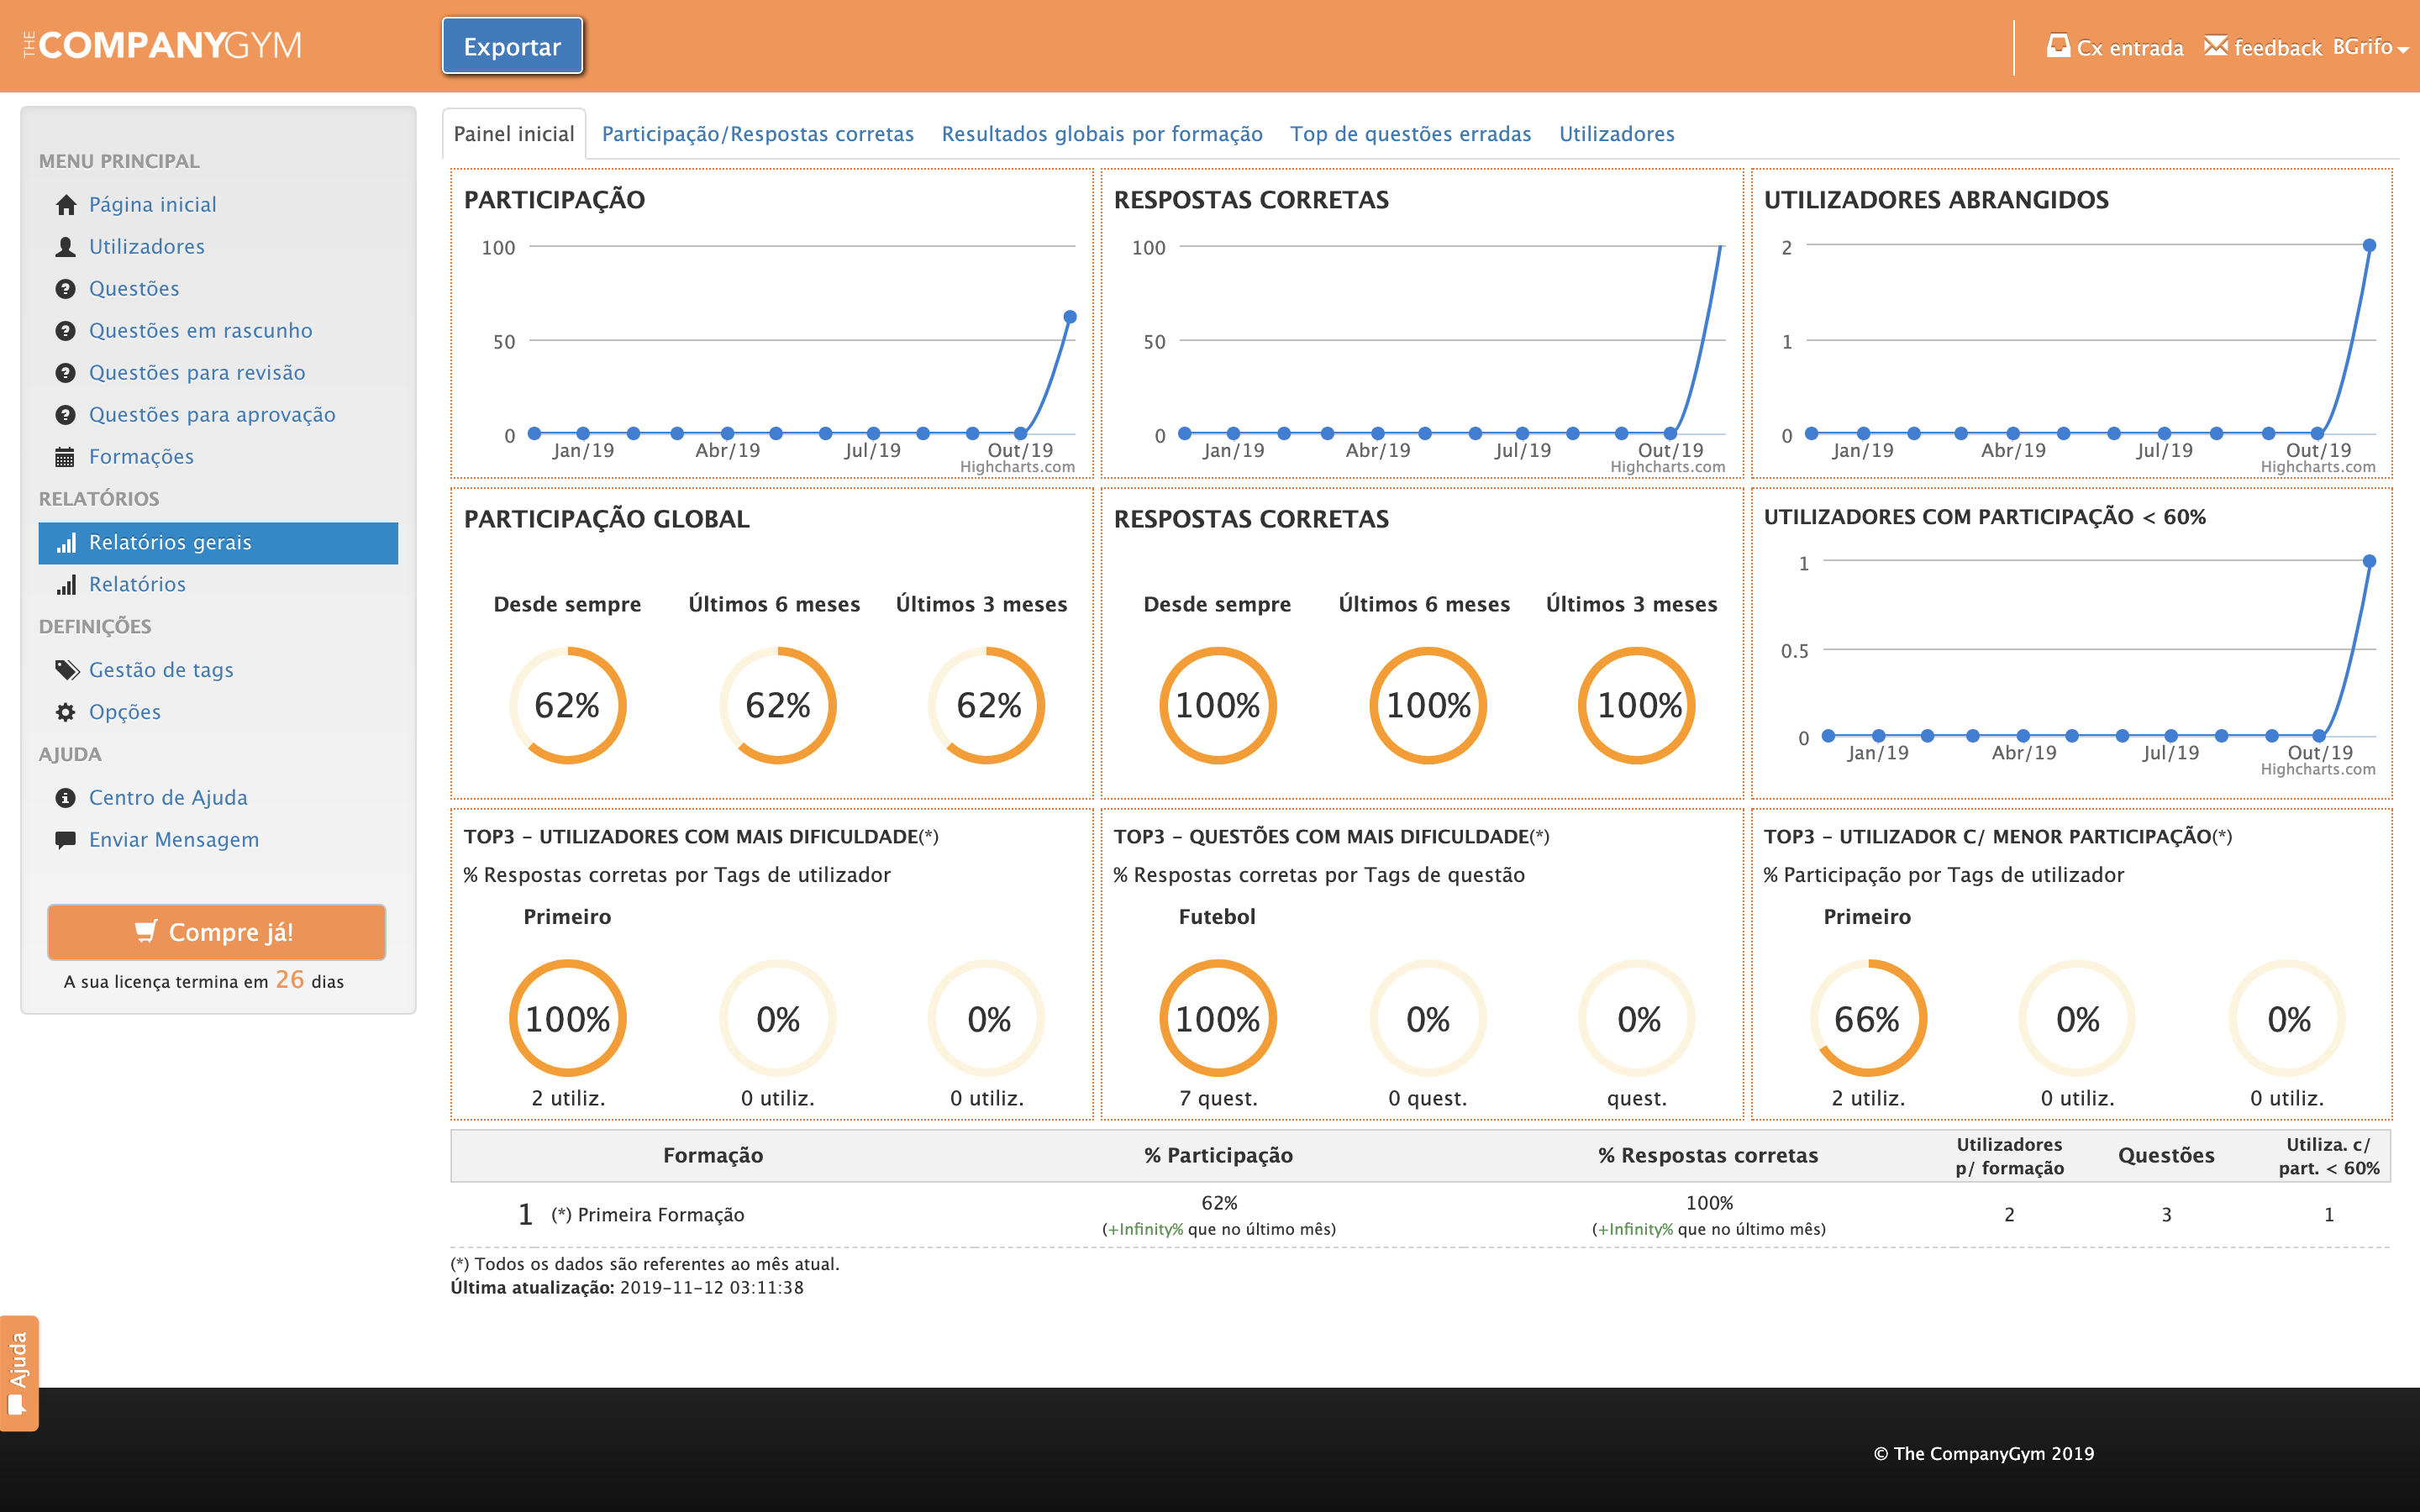
\includegraphics[width=1\textwidth]{img/tcg/tcg-homepage.png}
		\caption{The Company Gym - Página Inicial}
		\label{fig:tcg-homepage}
	\end{center}
\end{figure}

\begin{figure}[ht!]
	\begin{center}
		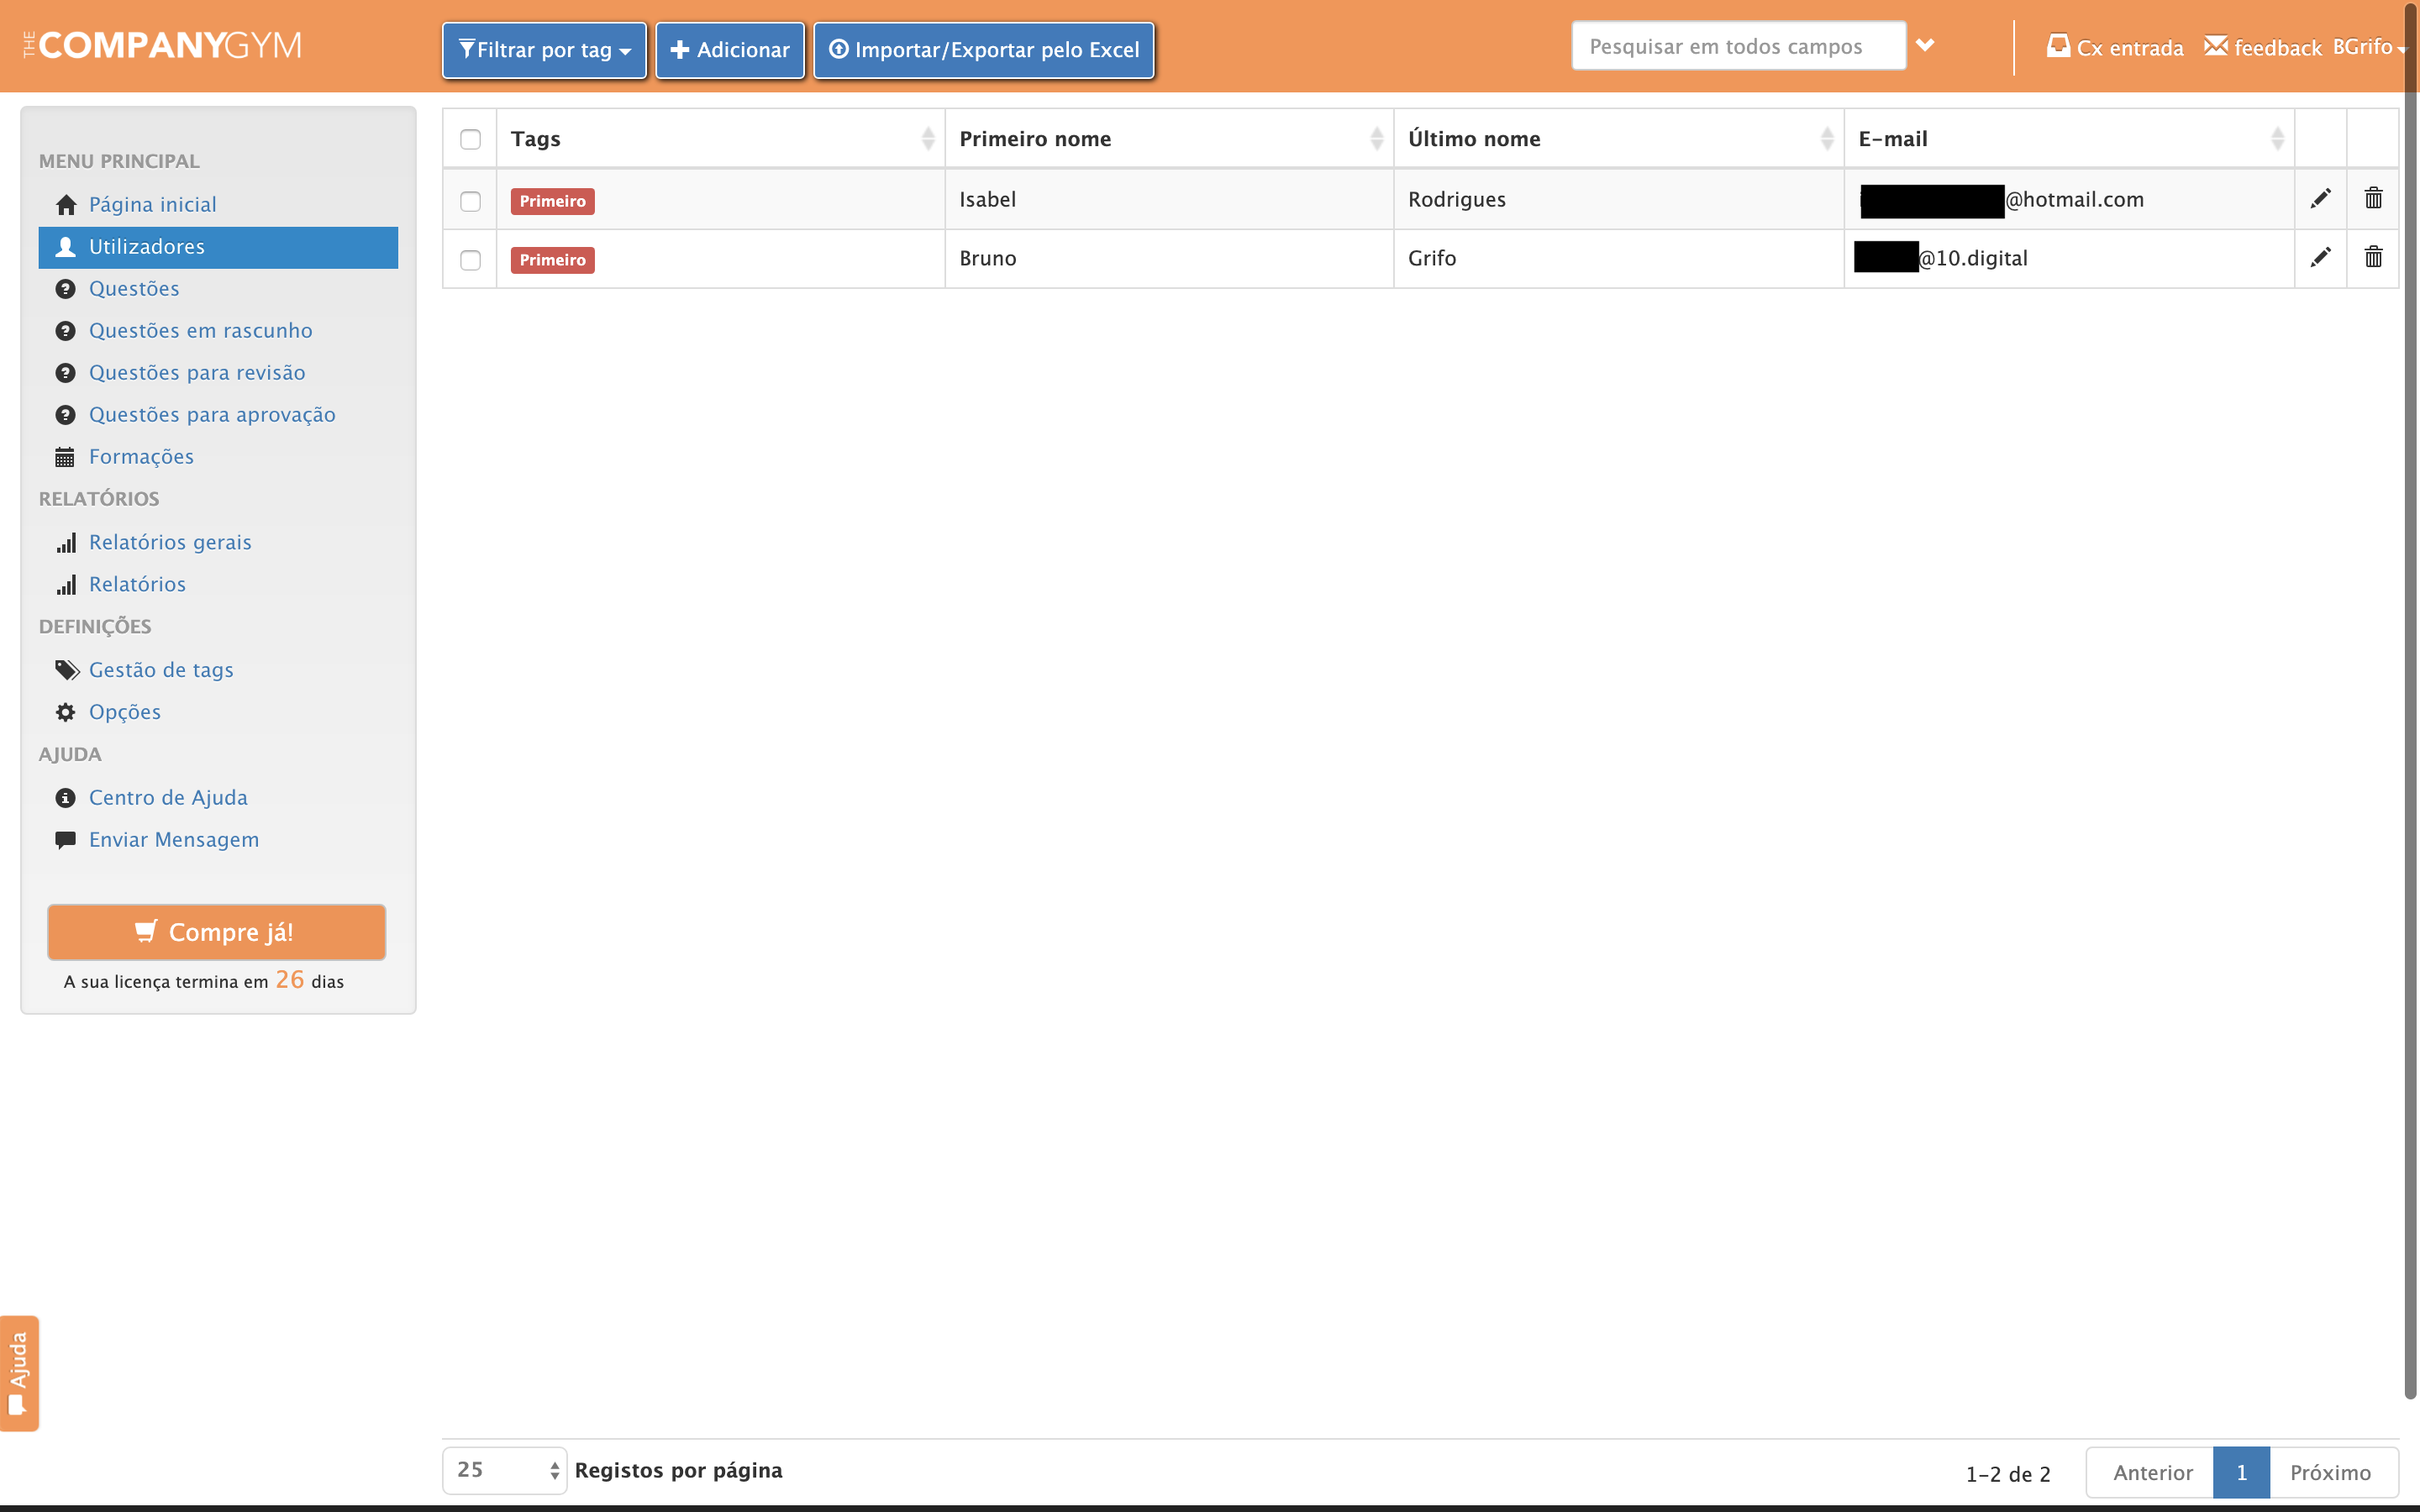
\includegraphics[width=1\textwidth]{img/tcg/tcg-utilizadores.png}
		\caption{The Company Gym - Lista de utilizadores finais}
		\label{fig:tcg-utilizadores}
	\end{center}
\end{figure}

Representado na Figura \ref{fig:tcg-utilizadores} está a lista de utilizadores finais. Para criar um novo utilizador final basta criar no botão "+Adicionar" e introduzir uma(s) tag, nova ou já existente, primeiro e ultimo nome e o e-mail por onde vai receber as formações. Como podemos ver há também um botão que permite importar uma lista de utilizadores finais e exportar a lista de utilizadores finais já adicionados no sistema, numa \textit{spreadsheet}.
\newpage

\begin{figure}[ht!]
	\begin{center}
		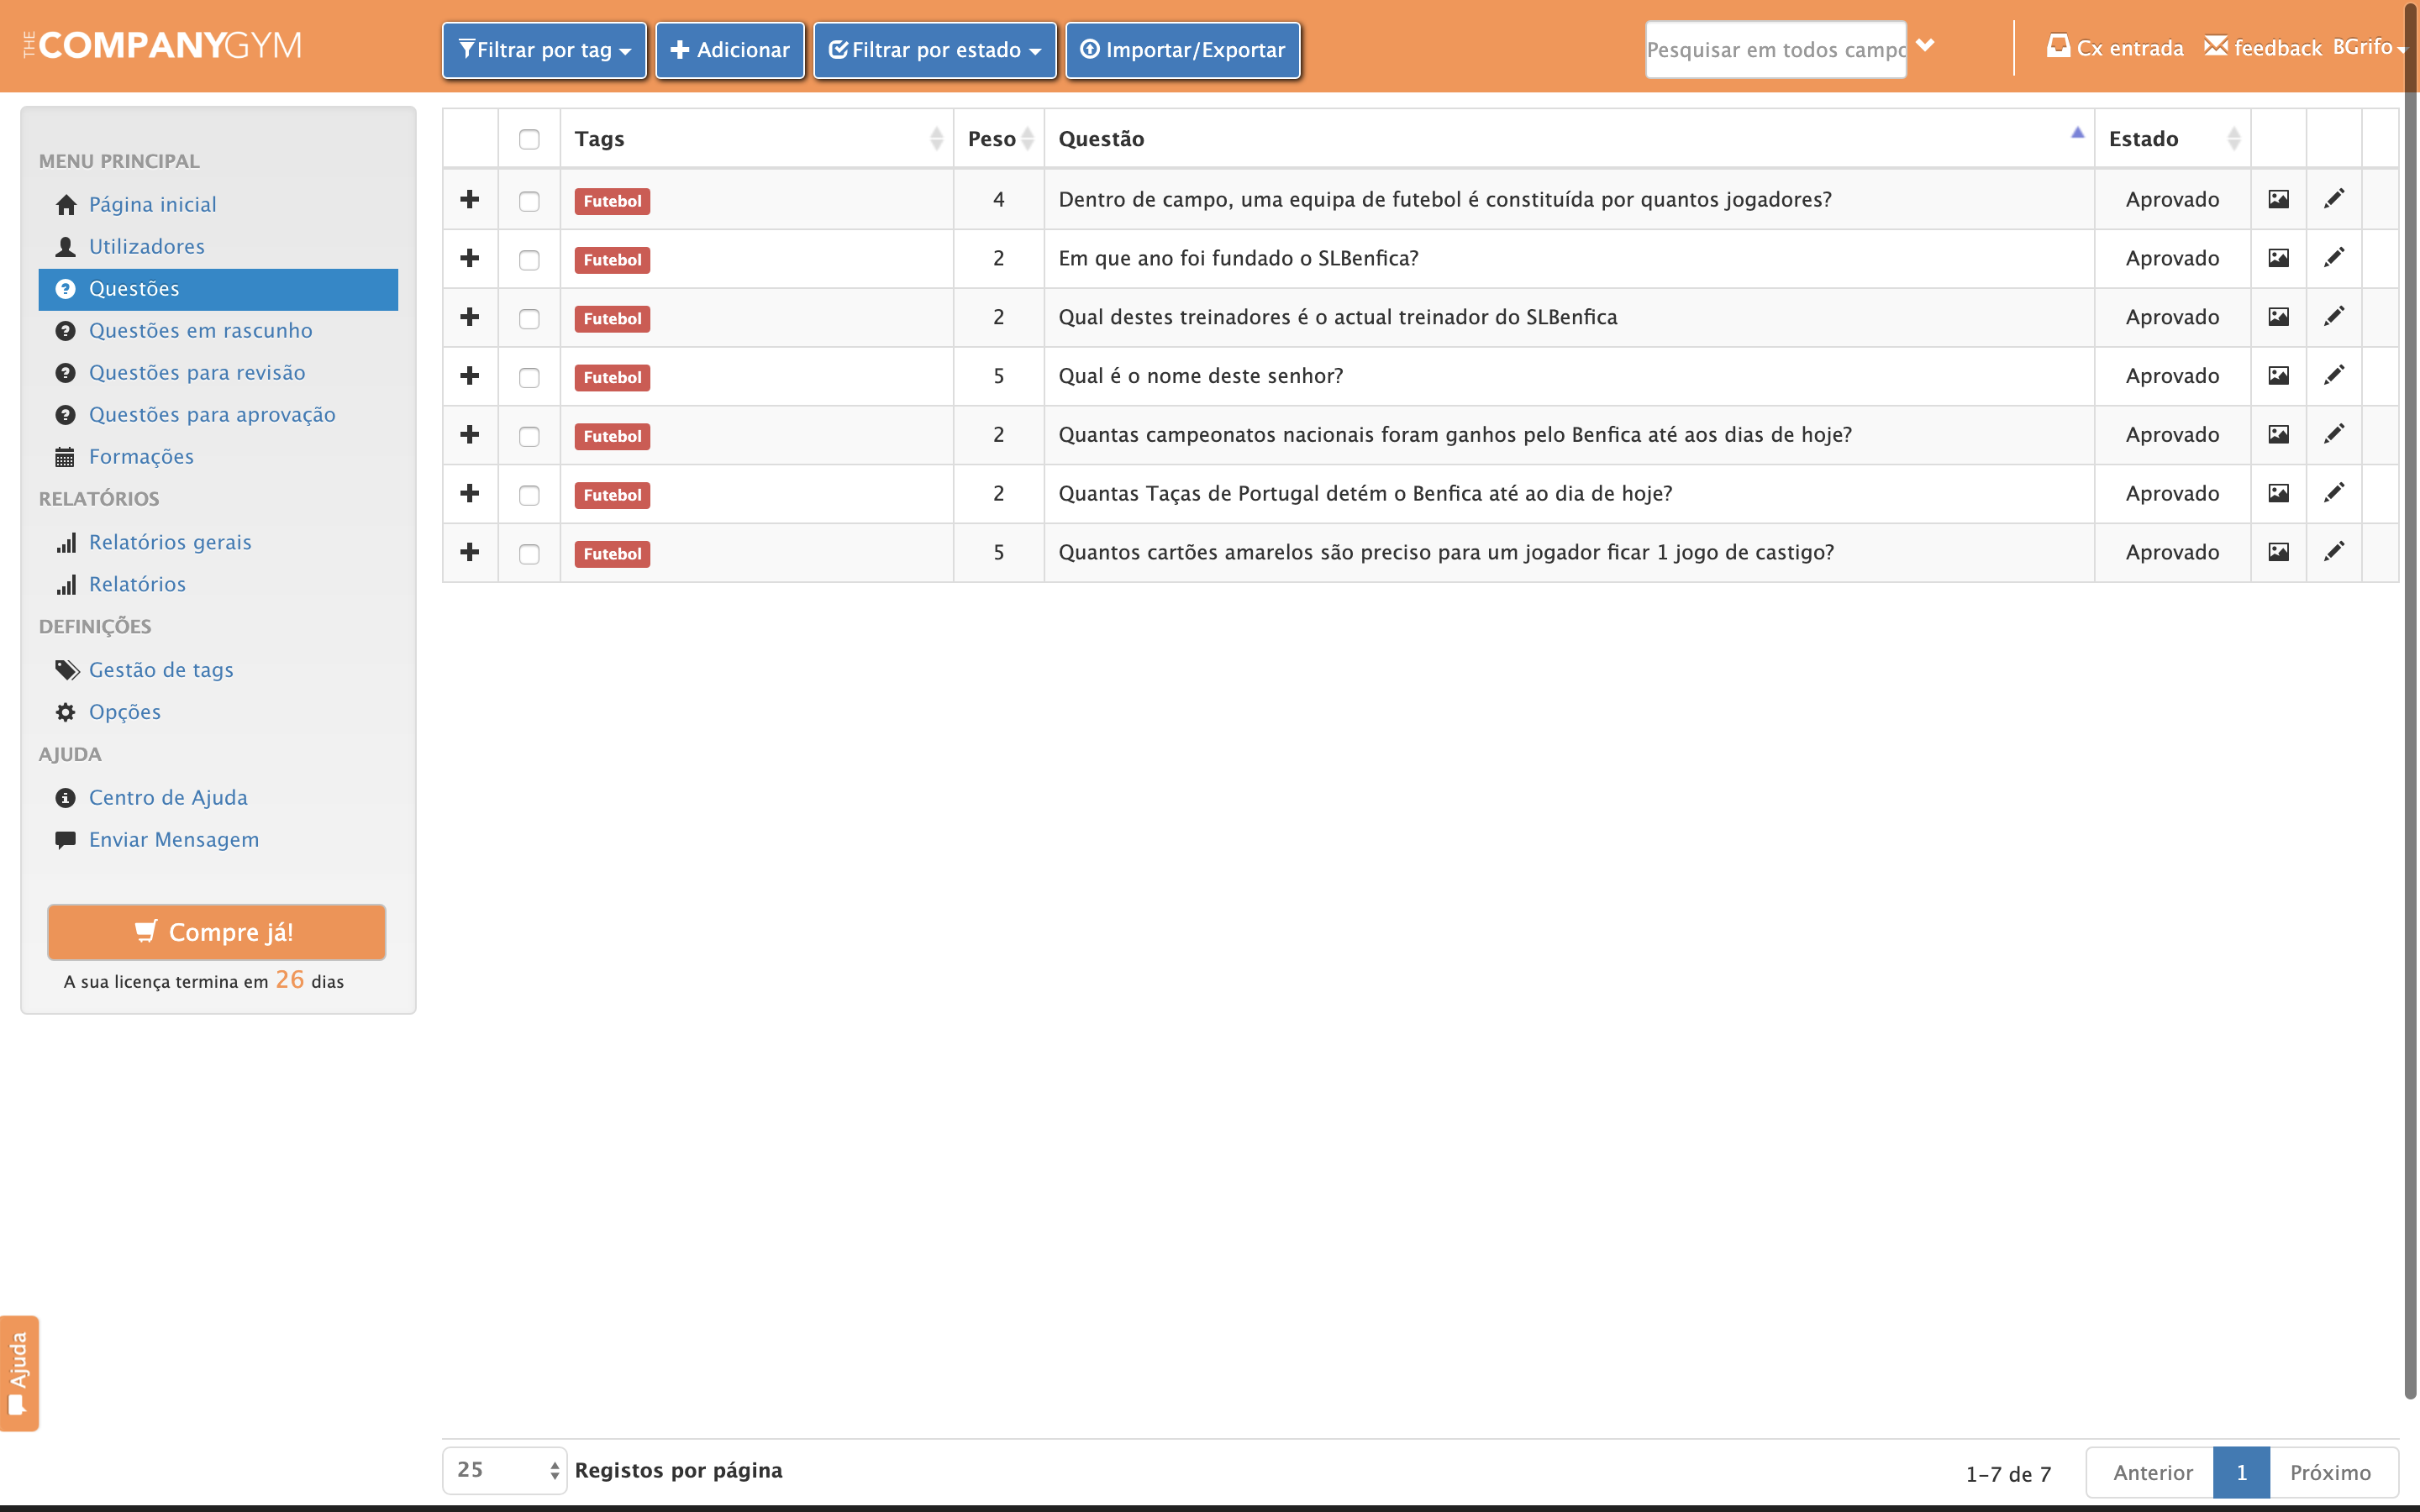
\includegraphics[width=1\textwidth]{img/tcg/tcg-questoes.png}
		\caption{The Company Gym - Lista de questões criadas}
		\label{fig:tcg-questoes}
	\end{center}
\end{figure}

\begin{figure}[ht!]
	\begin{center}
		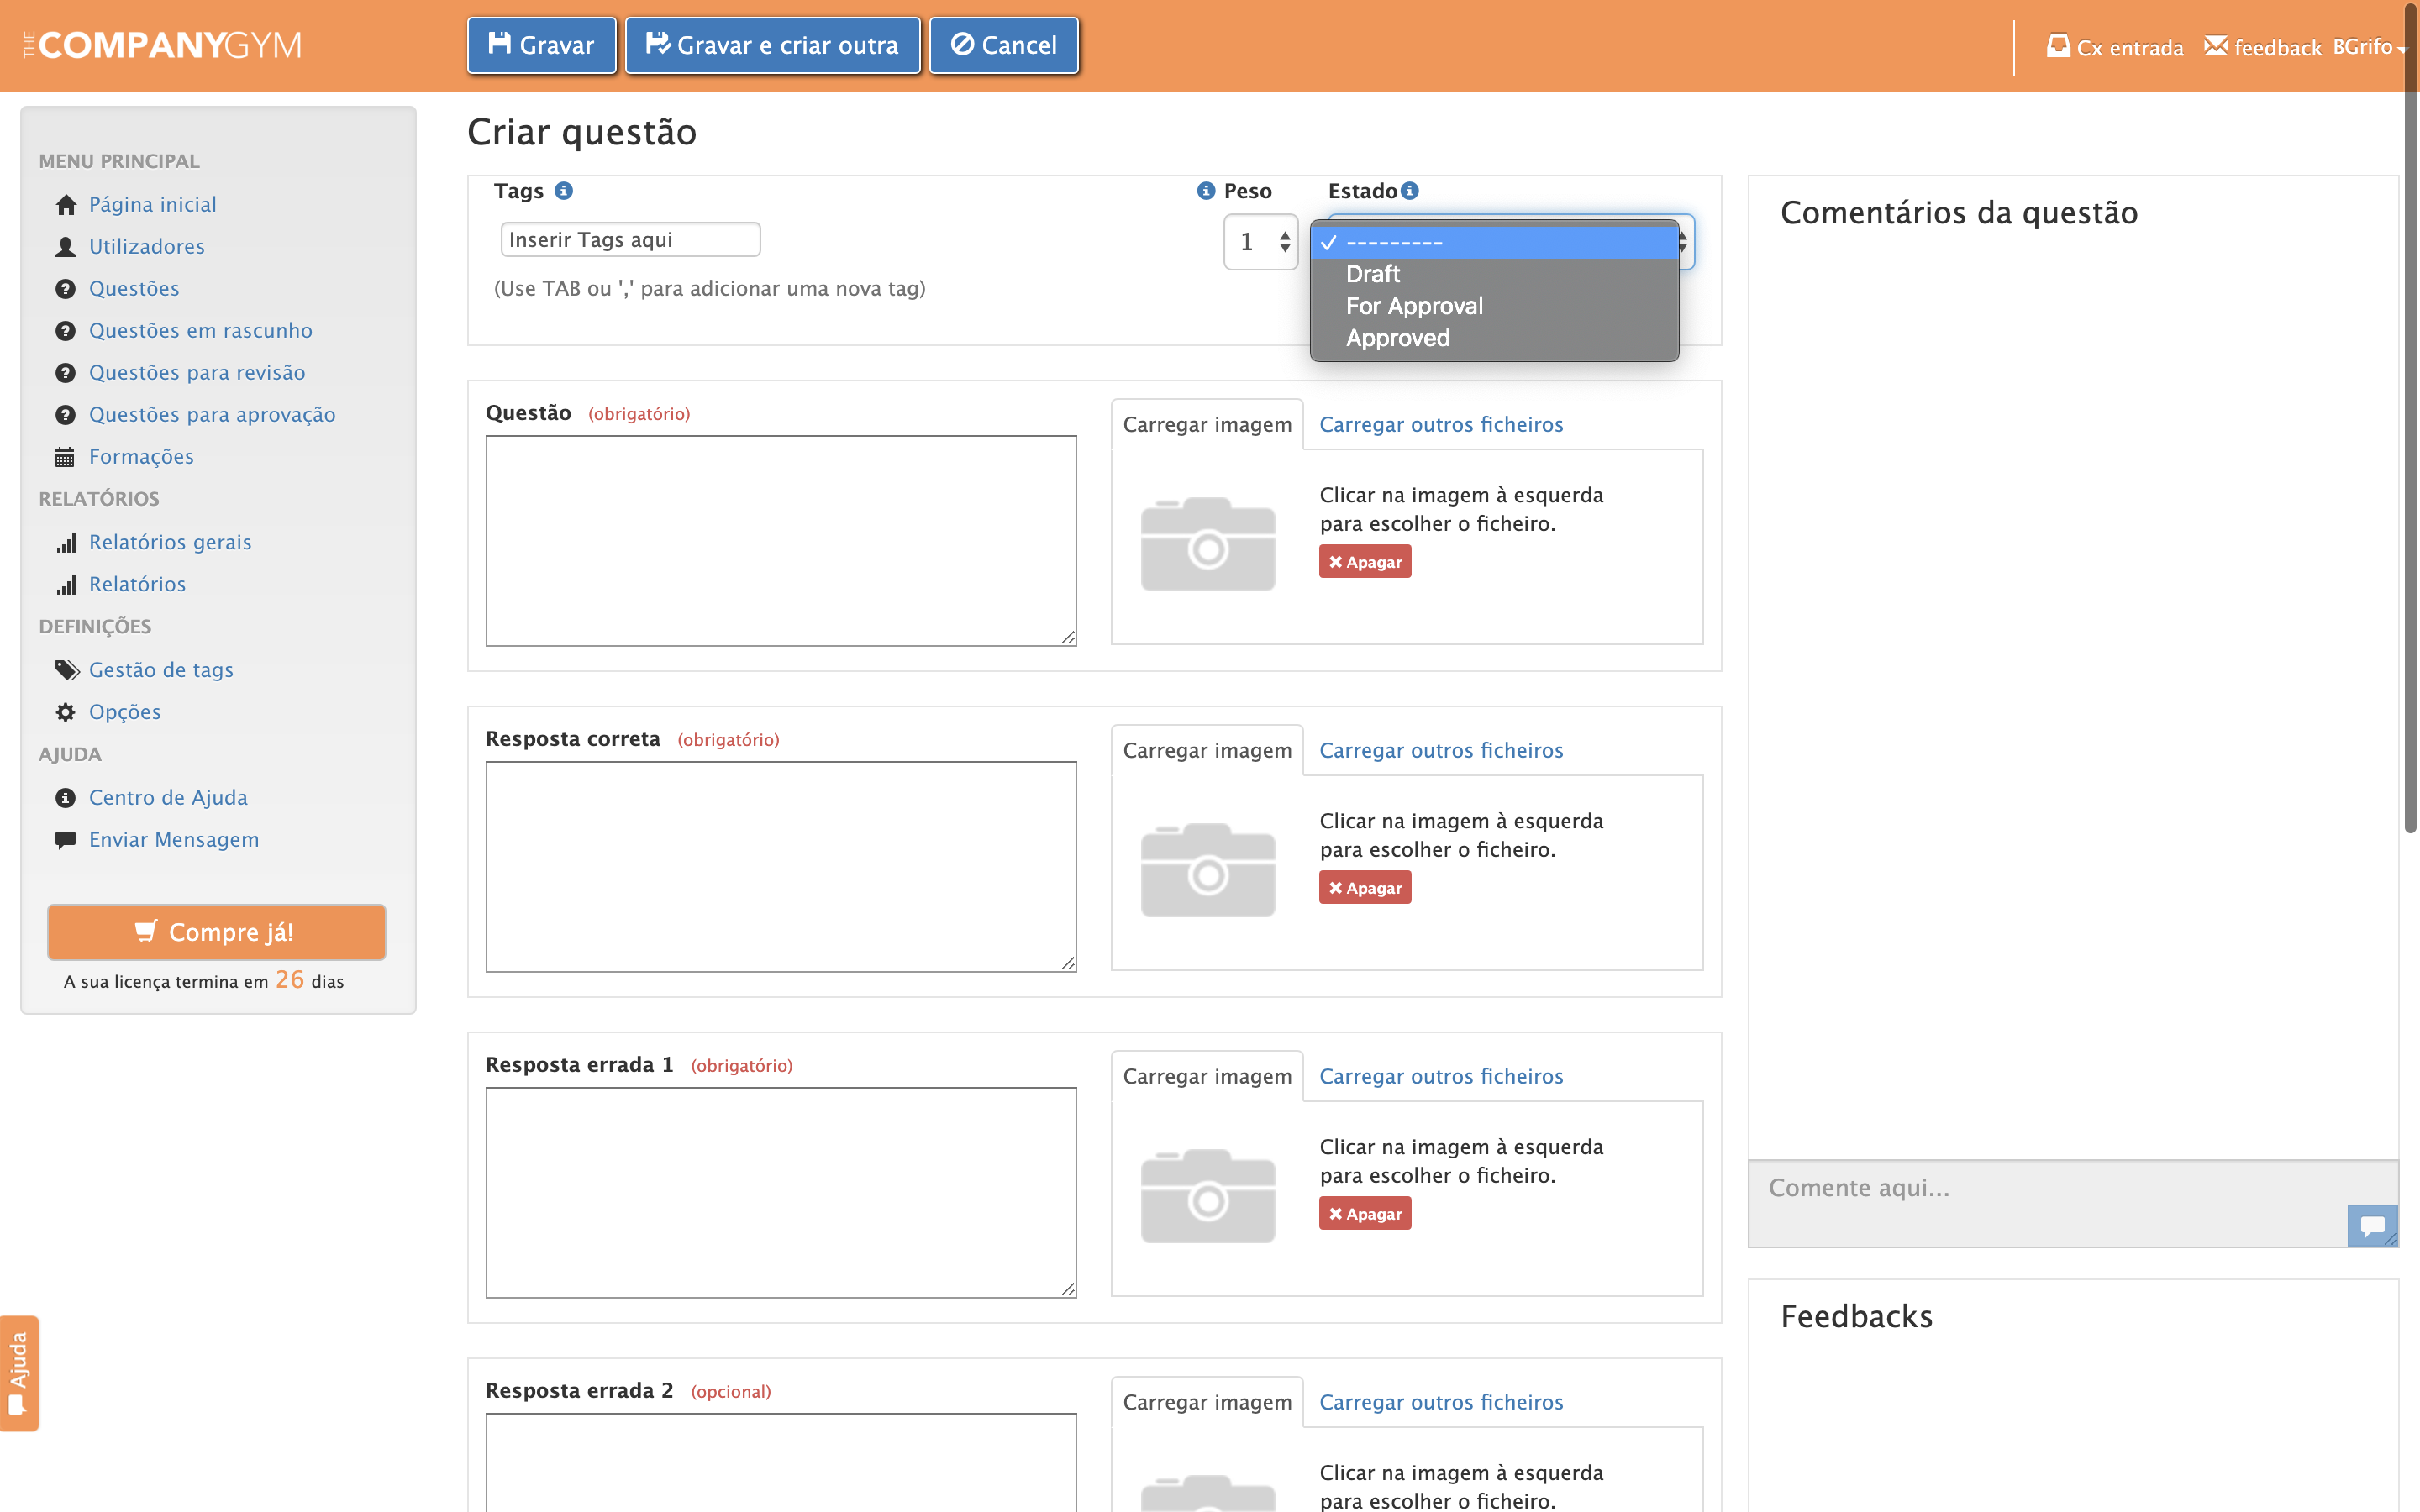
\includegraphics[width=1\textwidth]{img/tcg/tcg-criar-questao.png}
		\caption{The Company Gym - Criar questão}
		\label{fig:tcg-criar-questoes}
	\end{center}
\end{figure}

Na Figura \ref{fig:tcg-questoes} podemos ver que é possível listar todas as questão e filtra-las por \textit{tags} e estado. À semelhança do que acontece com os utilizadores, é também possível importar e exportar questões. Como podemos ver na Figura \ref{fig:tcg-criar-questoes} para criar uma nova questão é necessário atribuir uma(s) \textit{tag}, um peso (i. e. importância), um estado (\textit{draft}, \textit{for aproval} e \textit{aproved}), a questão e pelo menos duas respostas. Alguns alpectos como o anexo (i. e. imagem, video ou fichiero de som) na pergunta e/ou resposta são opcionais. Quando se importa uma serie de pergunas através de uma \textit{spreadsheet} todas as questões automaticamente ficam com estado \textit{draft} e como é de esperar sem anexos. Todas as questões que ficam em estado \textit{for aproval} terão de ser aprovadas pelo gestor de conta.


Nas Figuras \ref{fig:tcg-form}, \ref{fig:tcg-form1} e \ref{fig:tcg-form2} temos todas as fases para a criação de uma formação. Em primeiro lugar, é necessário definir a periocidade da formação.  Depois de escolher o nome é necessário dar um dia para o inicio e o fim da mesma, escolher os dias da semana em que o utilizador final irá receber a formação, a hora do dia a que recebe o mail e a duração (i. e. validade) que o utilizador tem para realizar a formação antes da mesma expirar. É de notar que a o sistema aceita uma duração com um max de horas igual à menor diferença entre os dias da semana escolhidos.

A seleção dos utilizadores finais e das questões faz-se através de tags. Desta forma temos uma forma bastante poderosa de adicionar multiplas questões e ao mesmo tempo escolher exatamente quais as questões que queremos numa formação e sem ter que fazer quaqueis alterações, adicionar e remover questões a qualquer hora. O mesmo se trata para os utilizadores finais. 



\begin{figure}[ht!]
	\begin{center}
		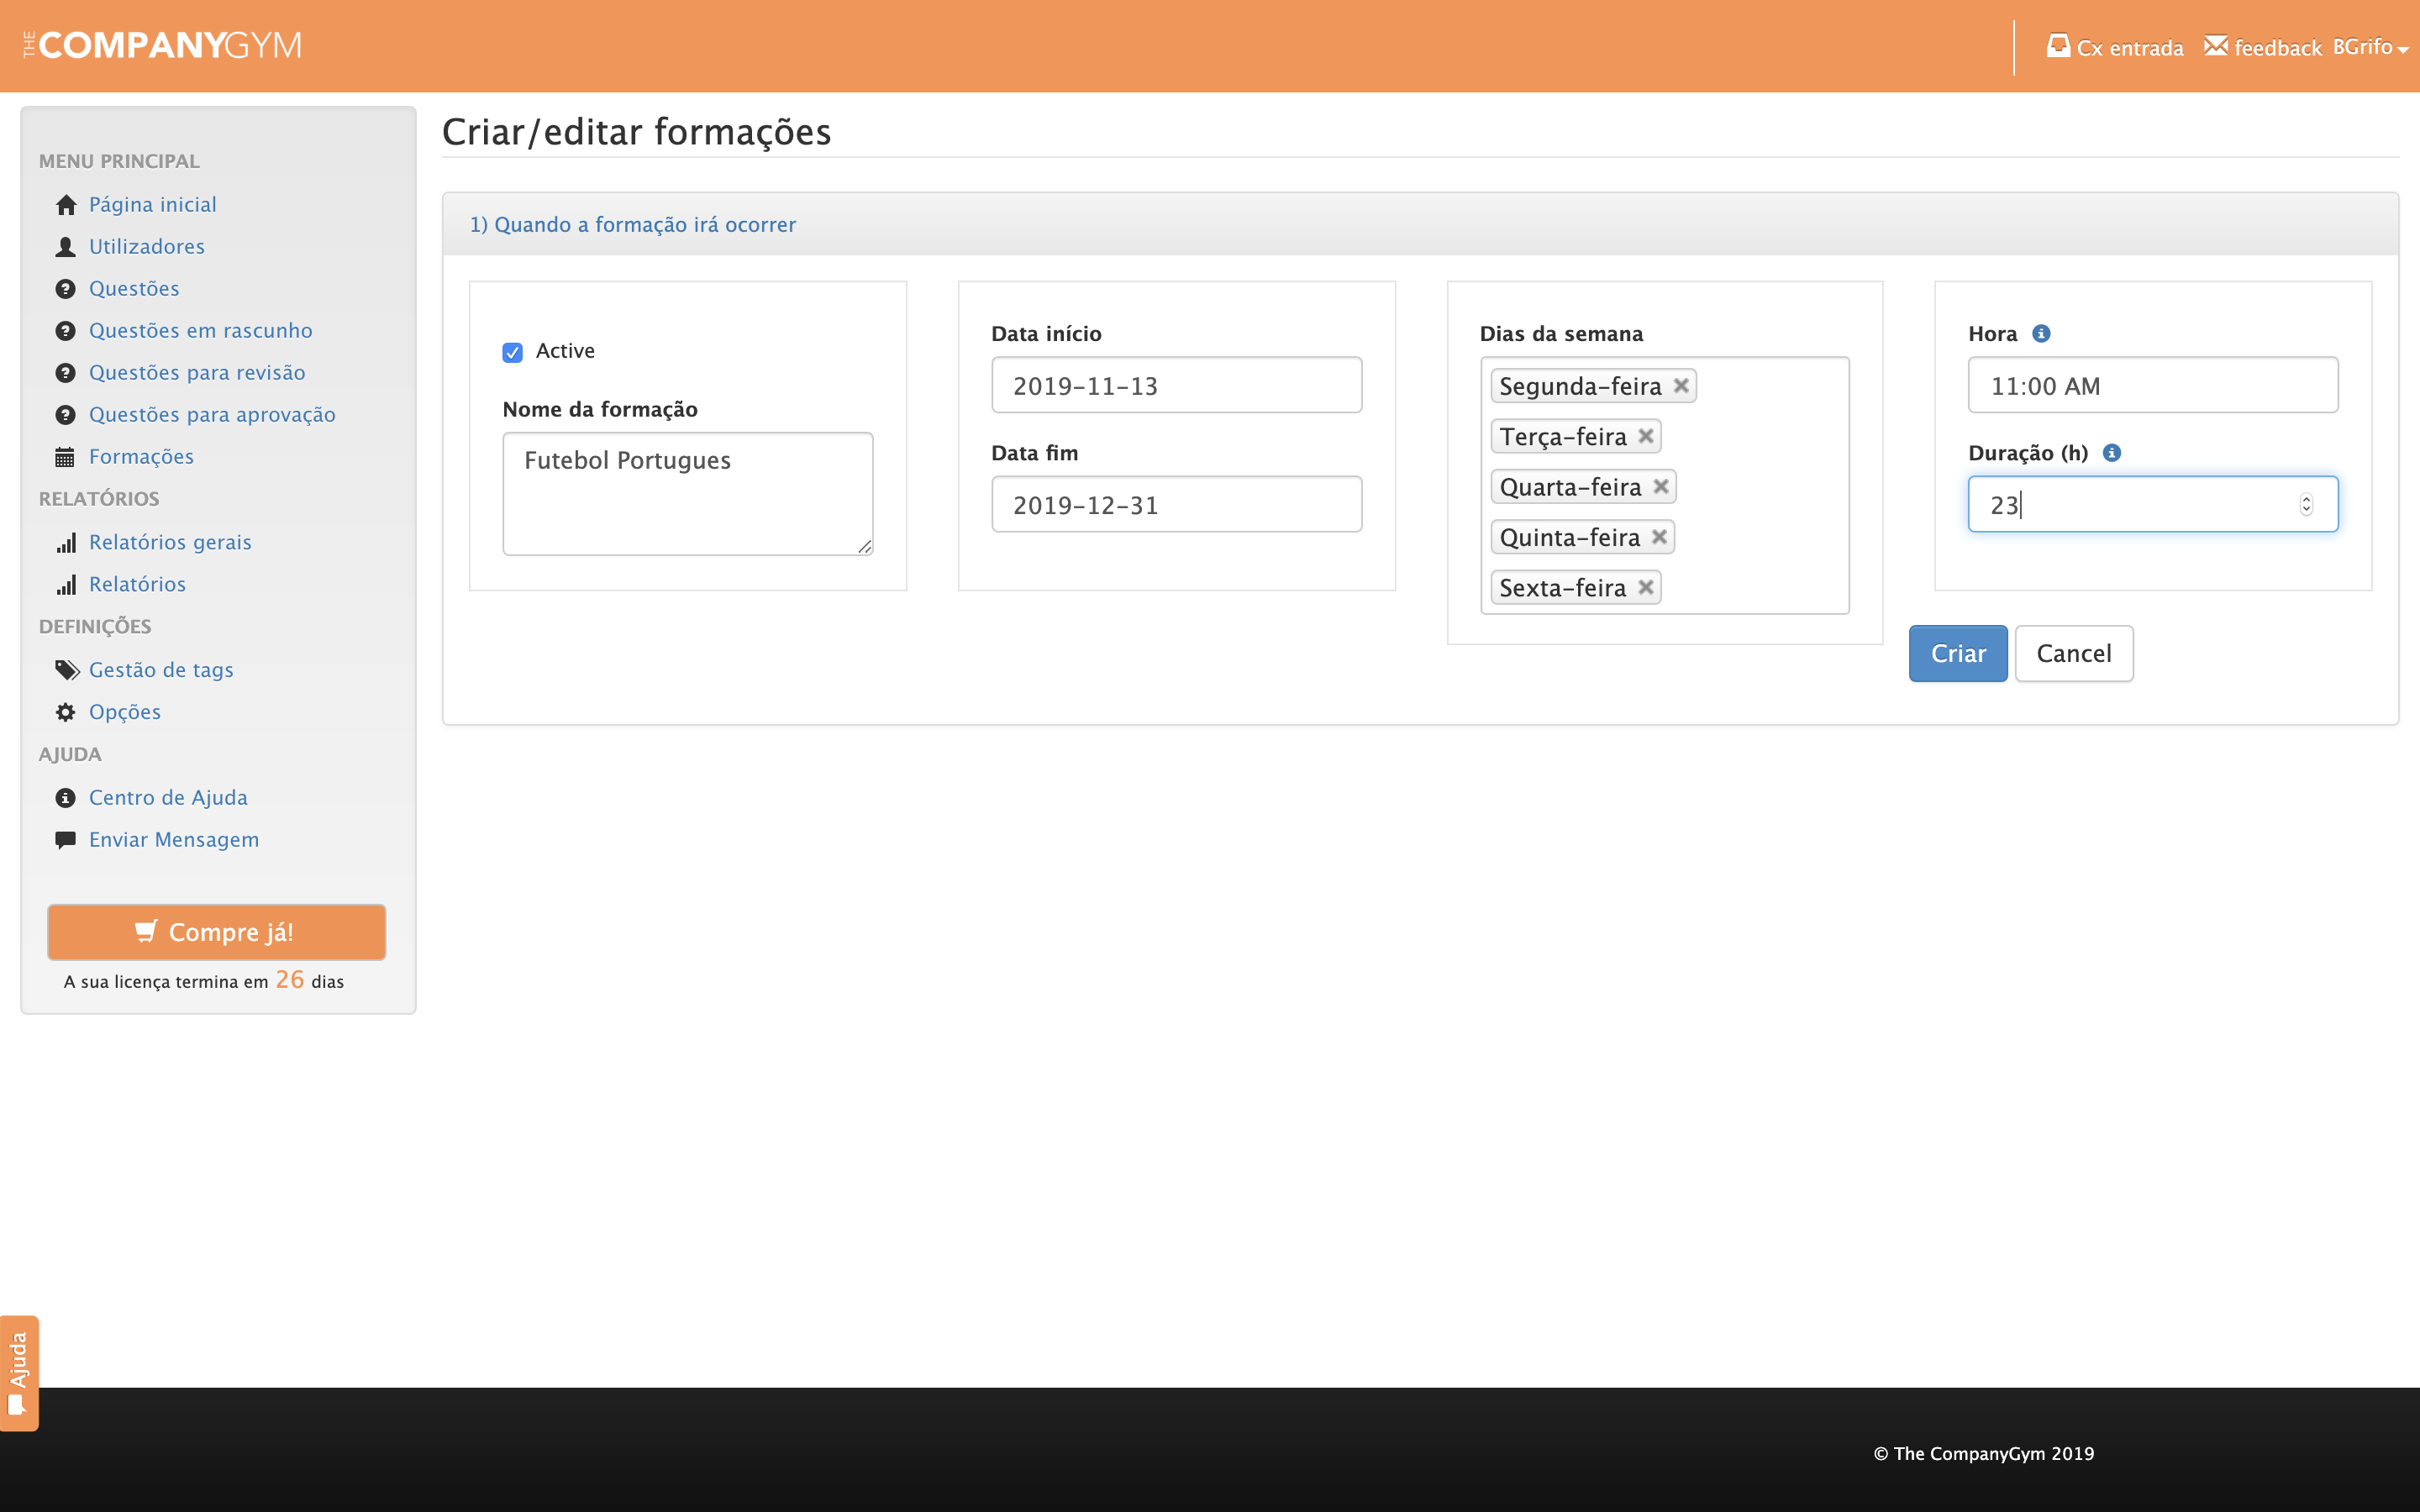
\includegraphics[width=1\textwidth]{img/tcg/tcg-form.png}
		\caption{The Company Gym - Criar Formação (Periodicidade)}
		\label{fig:tcg-form}
	\end{center}
\end{figure}

\newpage


\begin{figure}[ht!]
	\begin{center}
		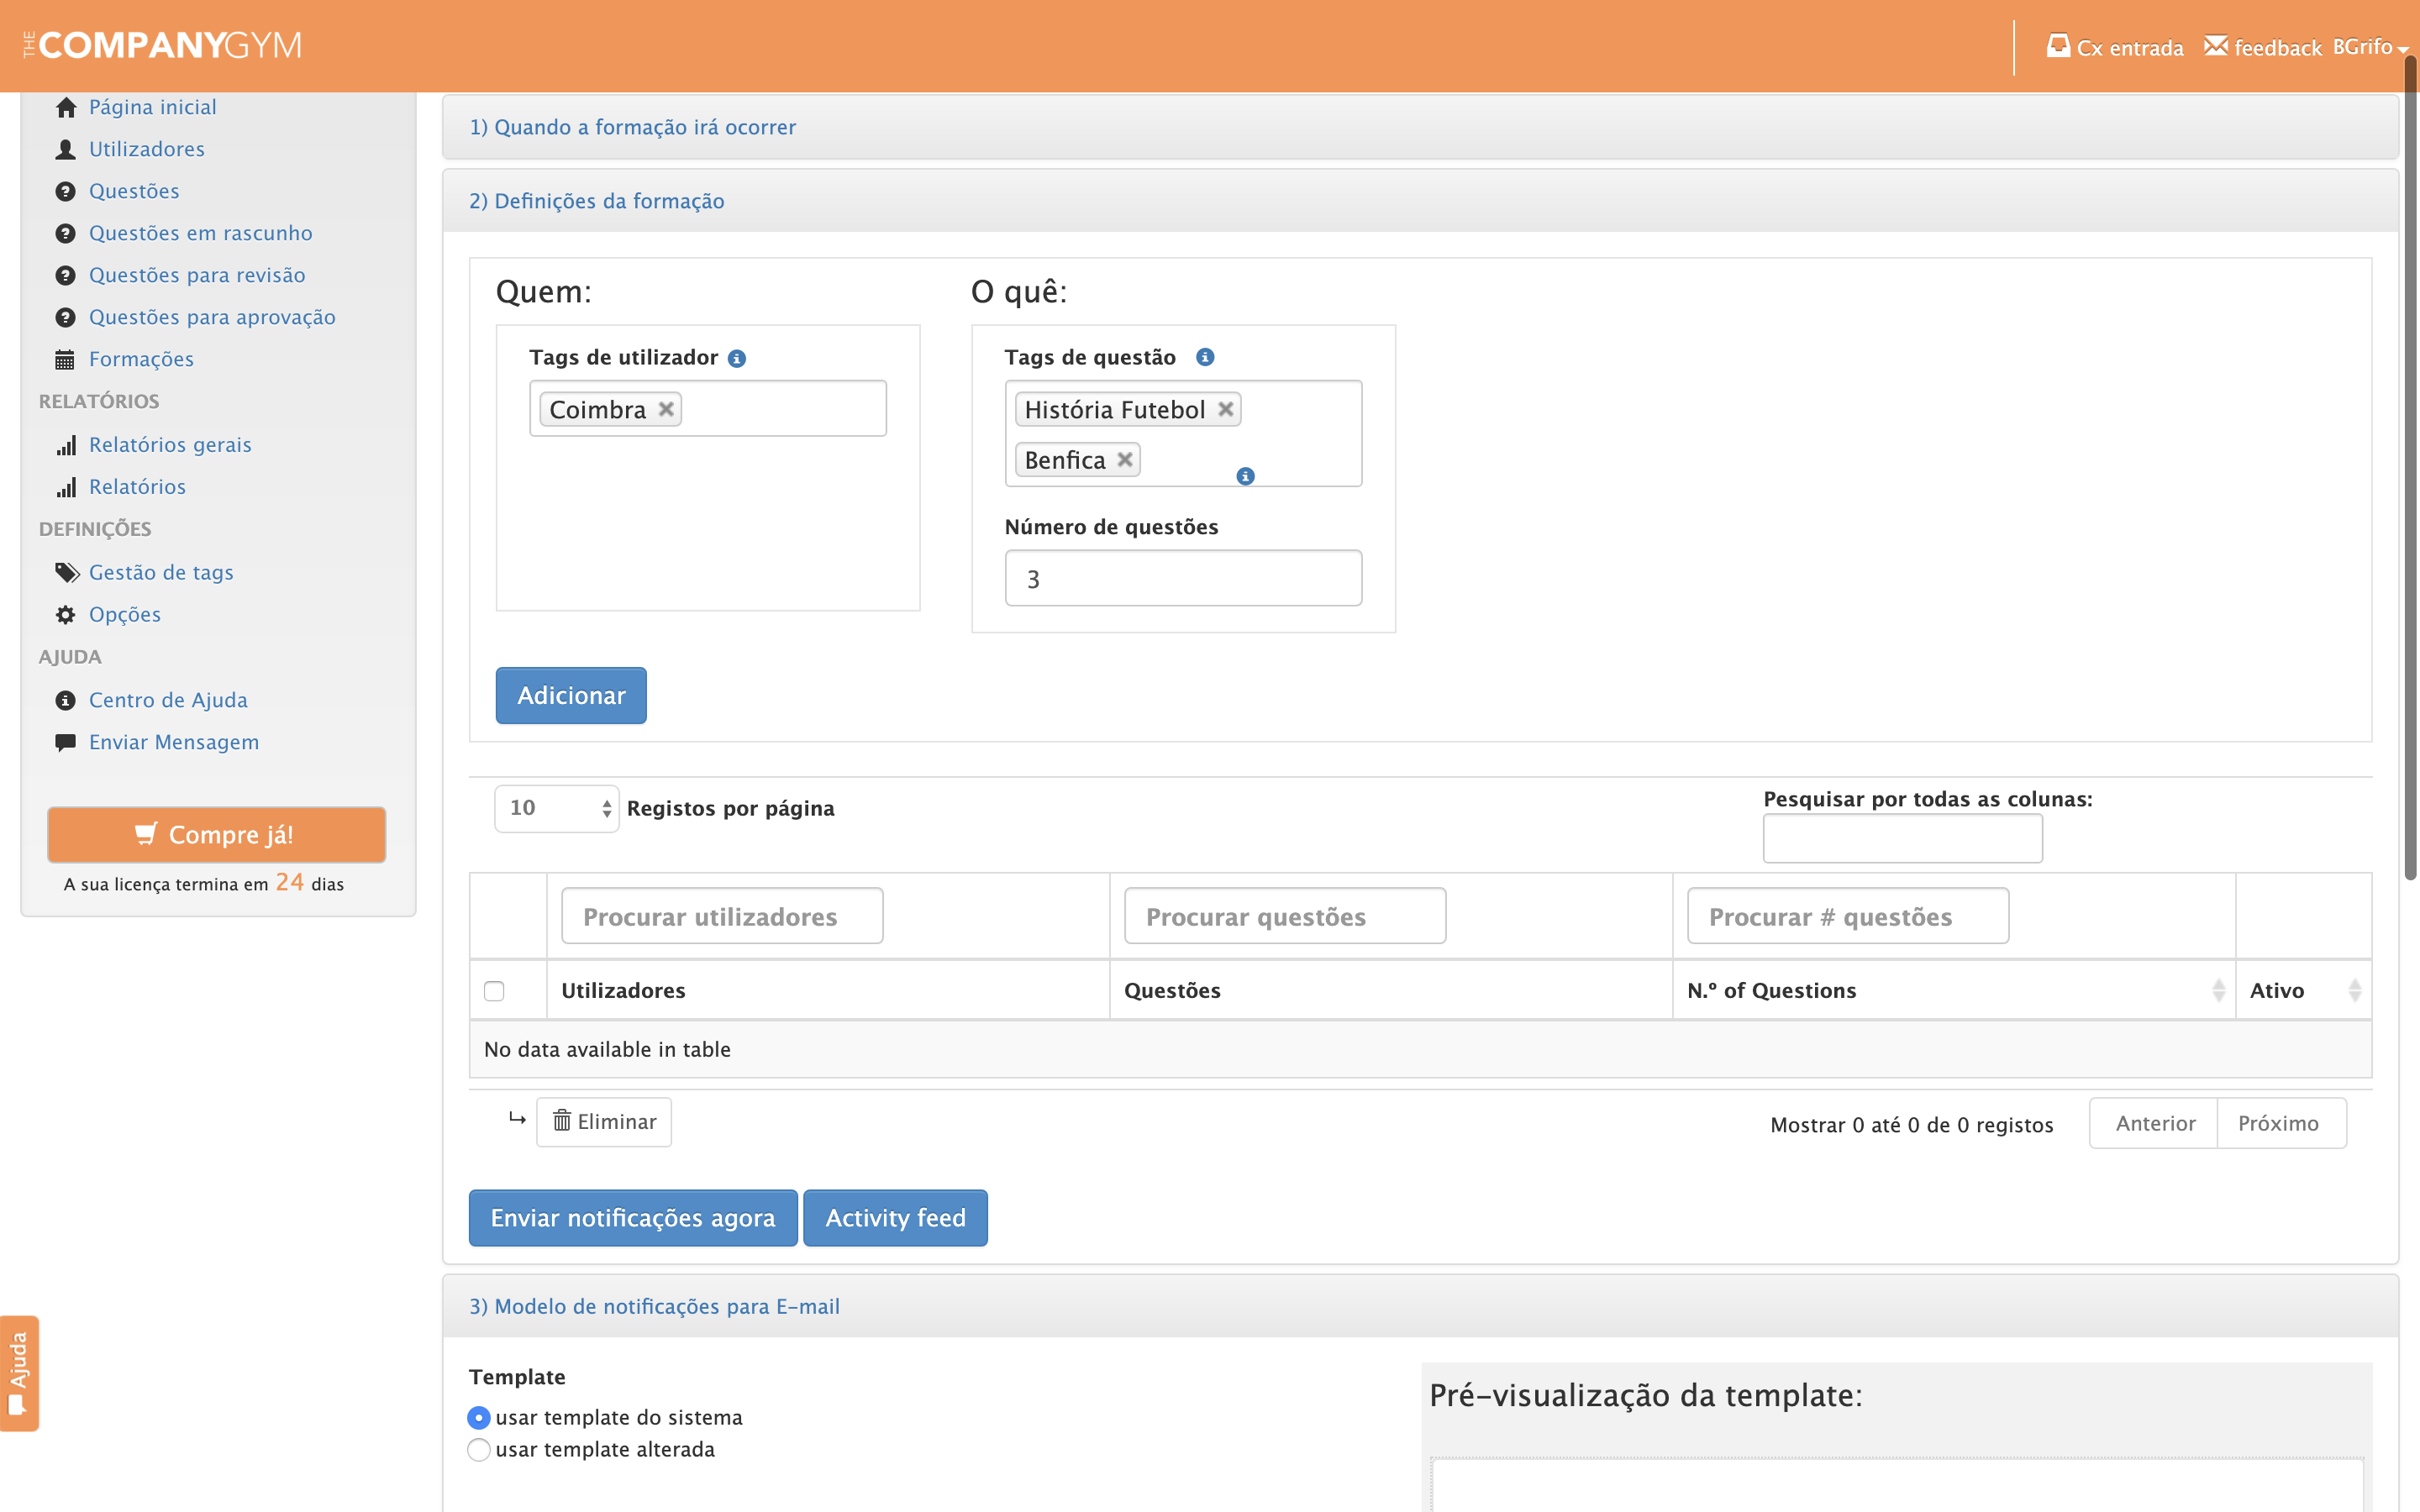
\includegraphics[width=1\textwidth]{img/tcg/tcg-form1.png}
		\caption{The Company Gym - Criar Formação (Definições)}
		\label{fig:tcg-form1}
	\end{center}
\end{figure}

\begin{figure}[ht!]
	\begin{center}
		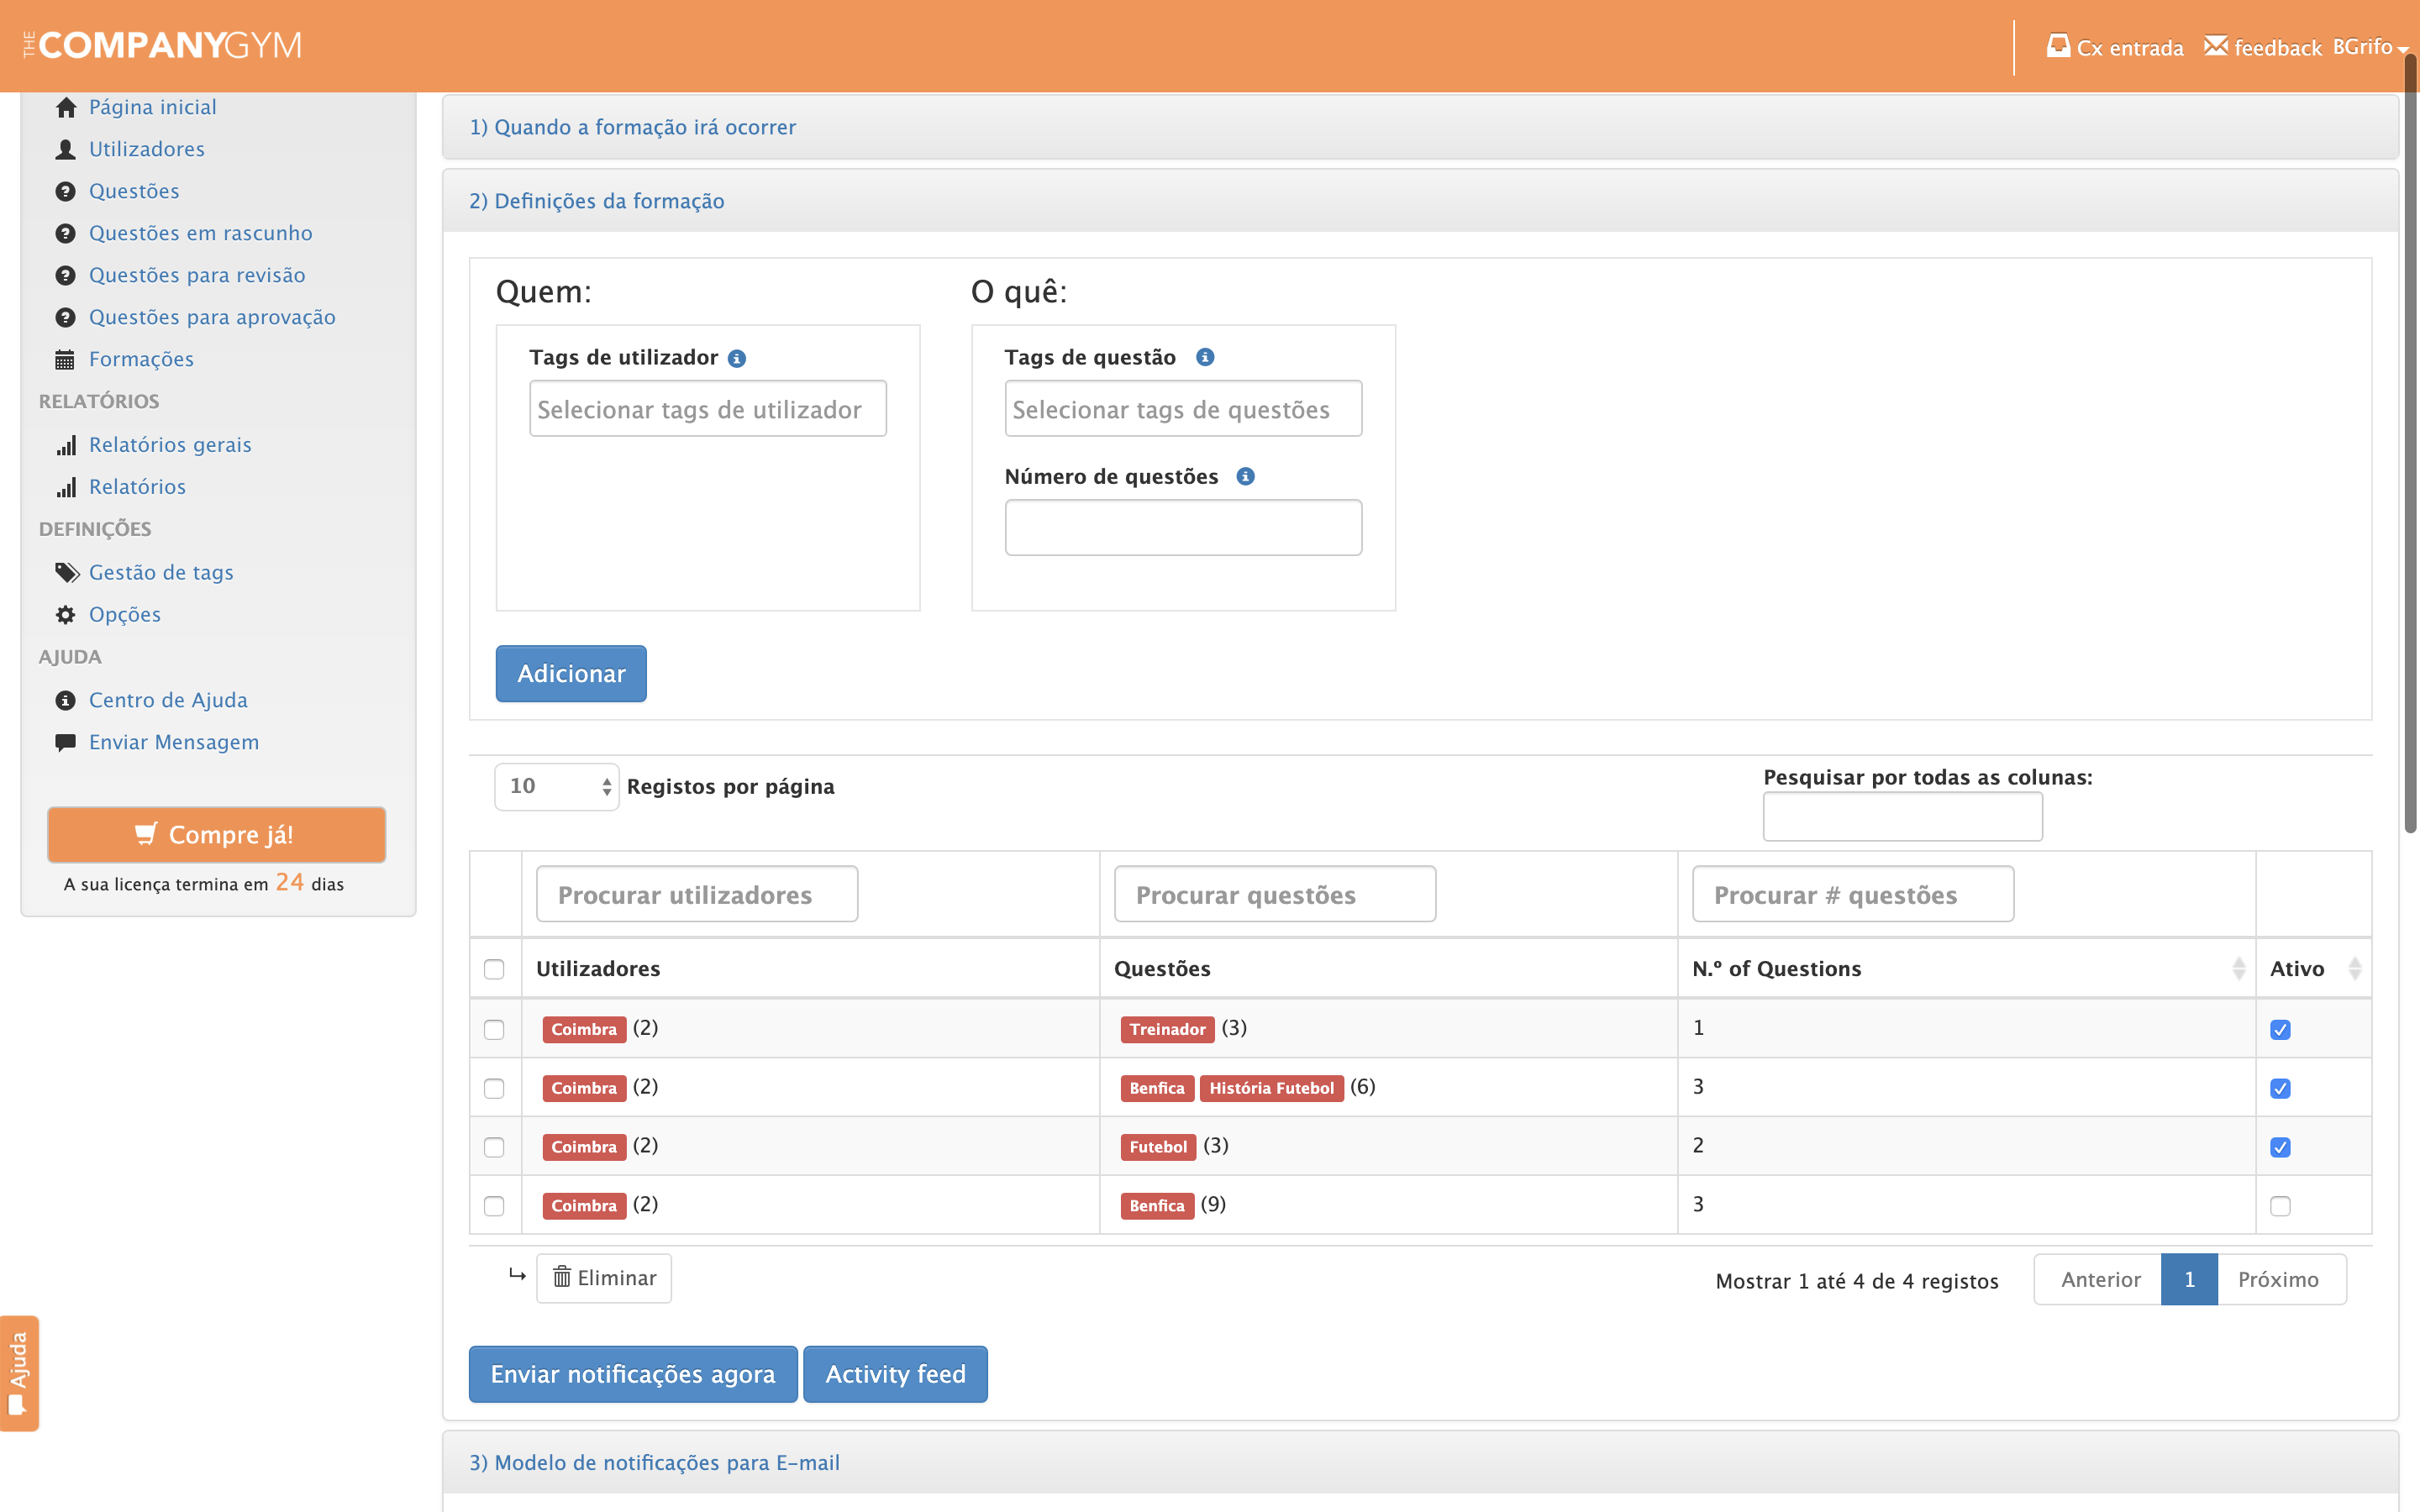
\includegraphics[width=1\textwidth]{img/tcg/tcg-form2.png}
		\caption{The Company Gym - Criar Formação (Gerir Utilizadores e Questões)}
		\label{fig:tcg-form2}
	\end{center}
\end{figure}

O botão "Activity feed" abre uma nova janela com o histórico de actividades da formação como podemos ver na Figura \ref{fig:tcg-feed}. O historico pode ser organizado pelas caracteristica de cada coluna e para cada registo, é possível ver verificar as respostas do utilizador final na formação.


\begin{figure}[ht!]
	\begin{center}
		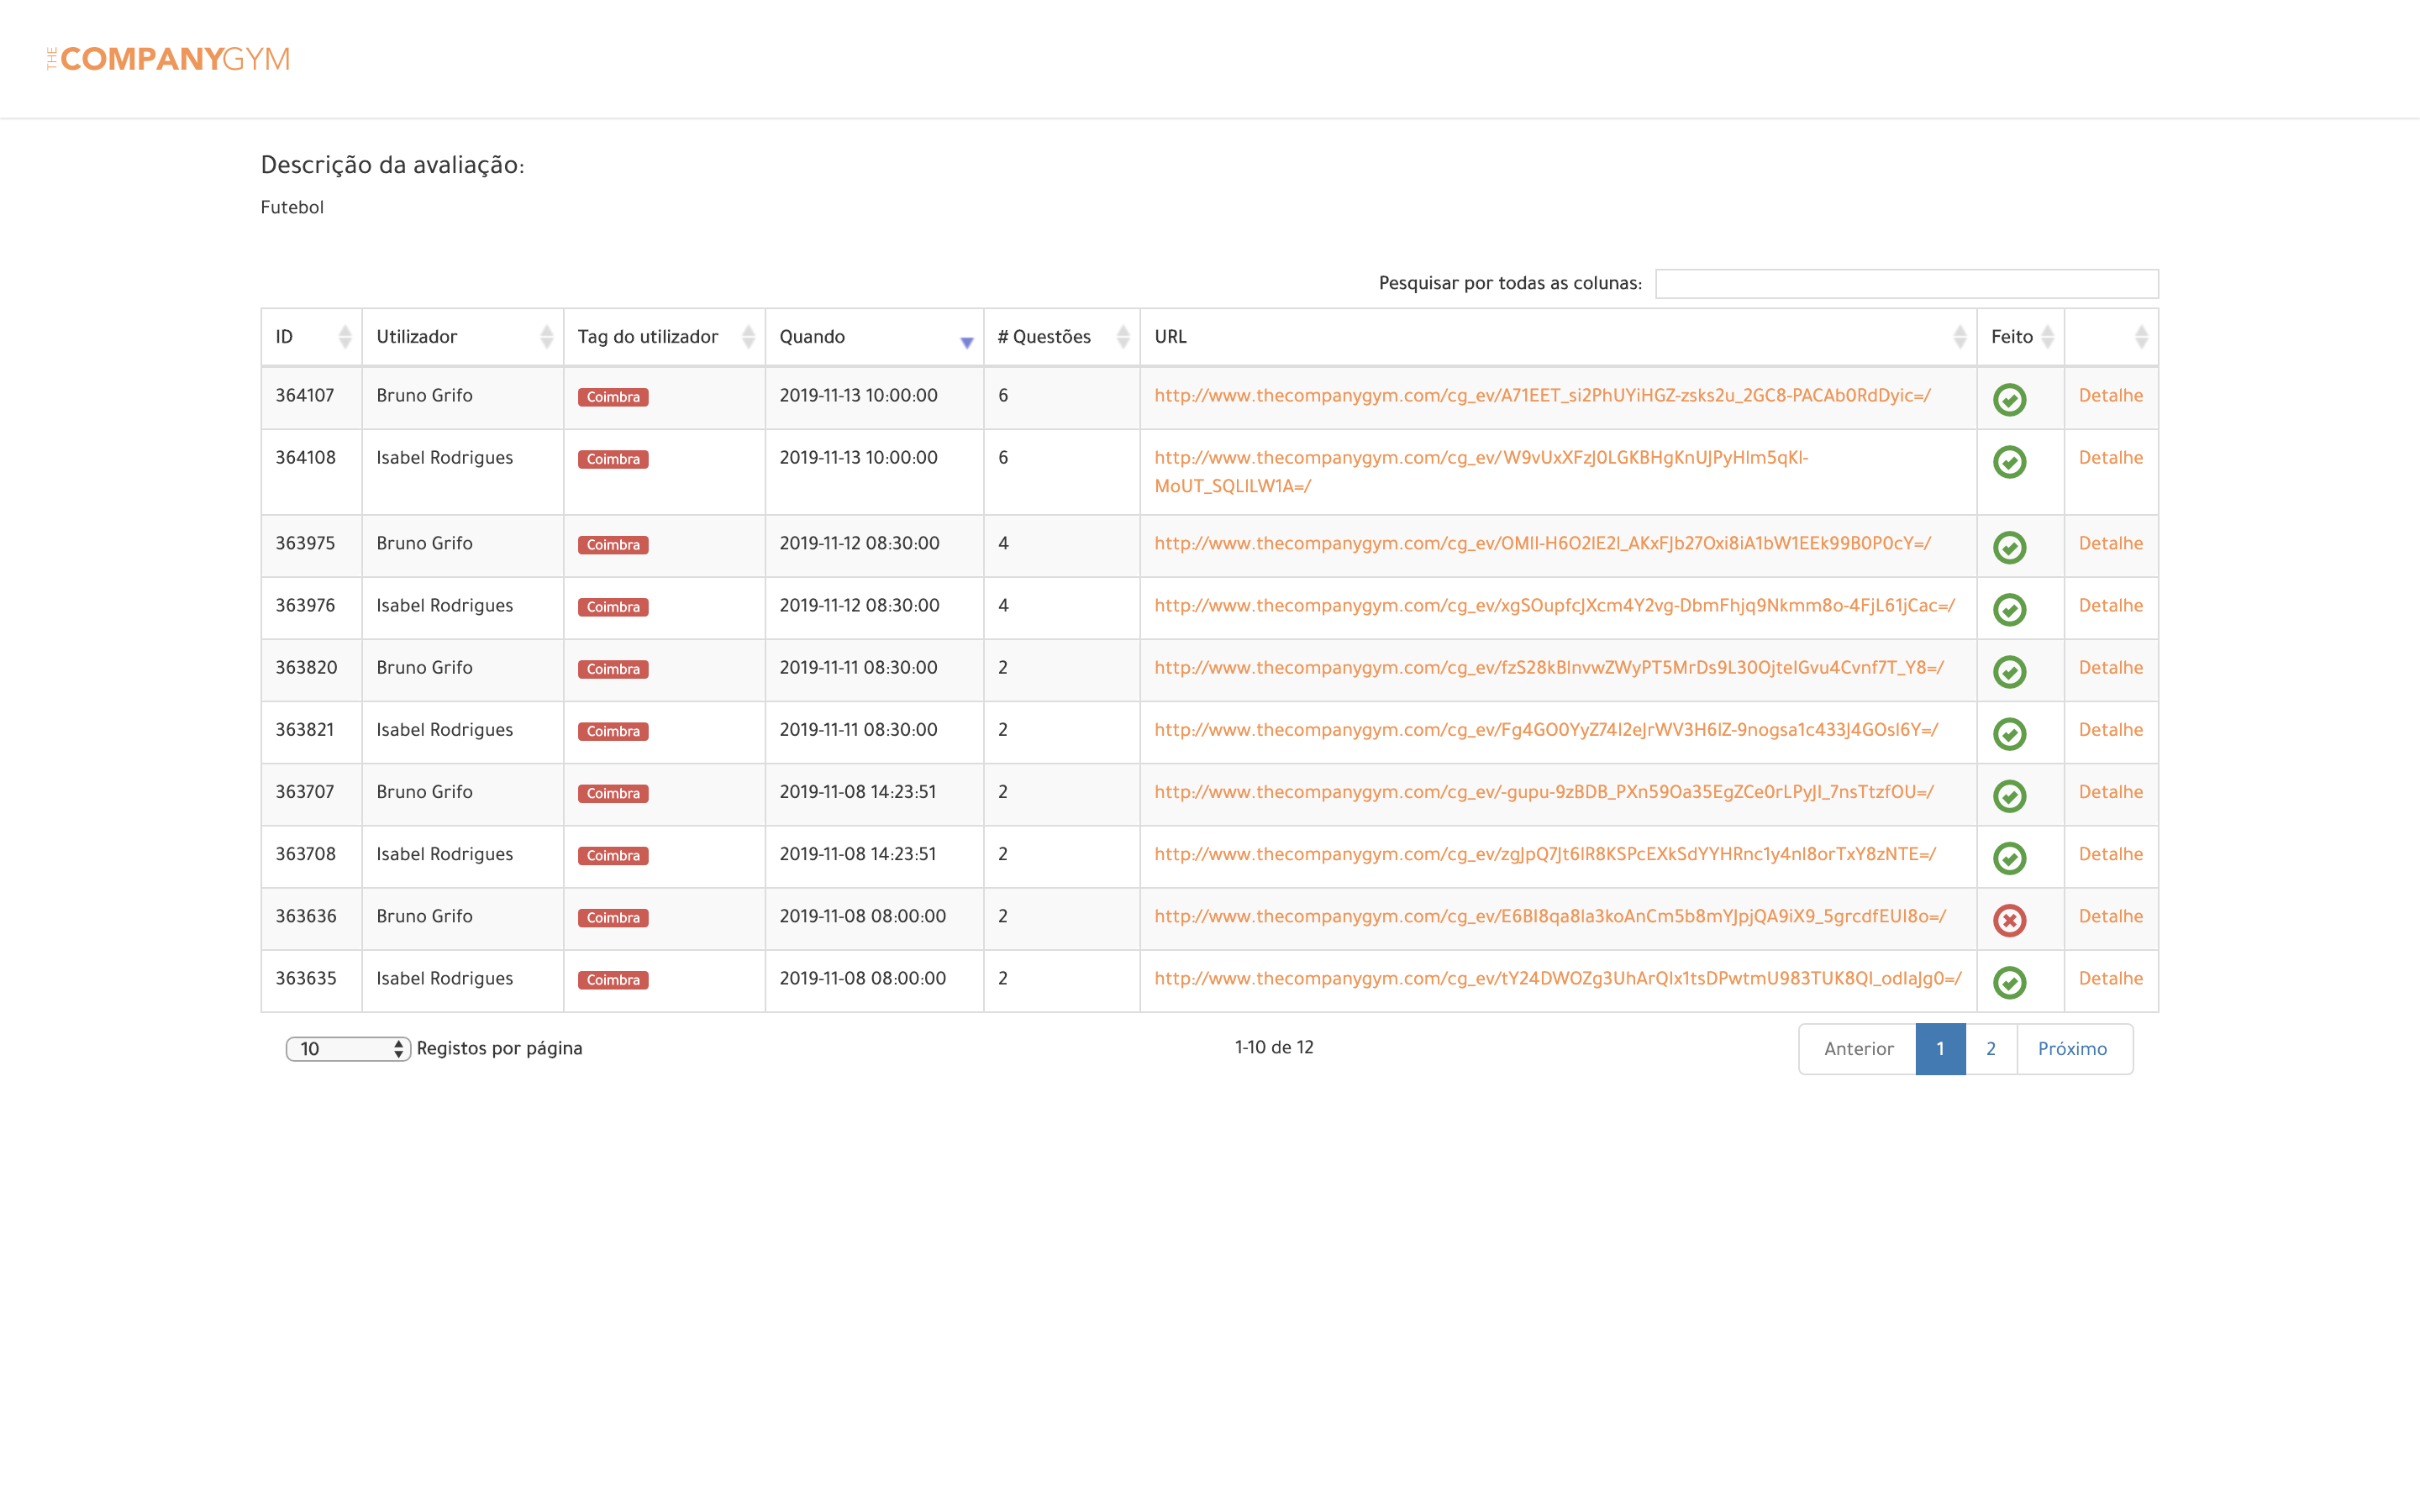
\includegraphics[width=1\textwidth]{img/tcg/tcg-feed.png}
		\caption{The Company Gym - Histórico de actividades}
		\label{fig:tcg-feed}
	\end{center}
\end{figure}

\newpage


\begin{figure}[ht!]
	\begin{center}
		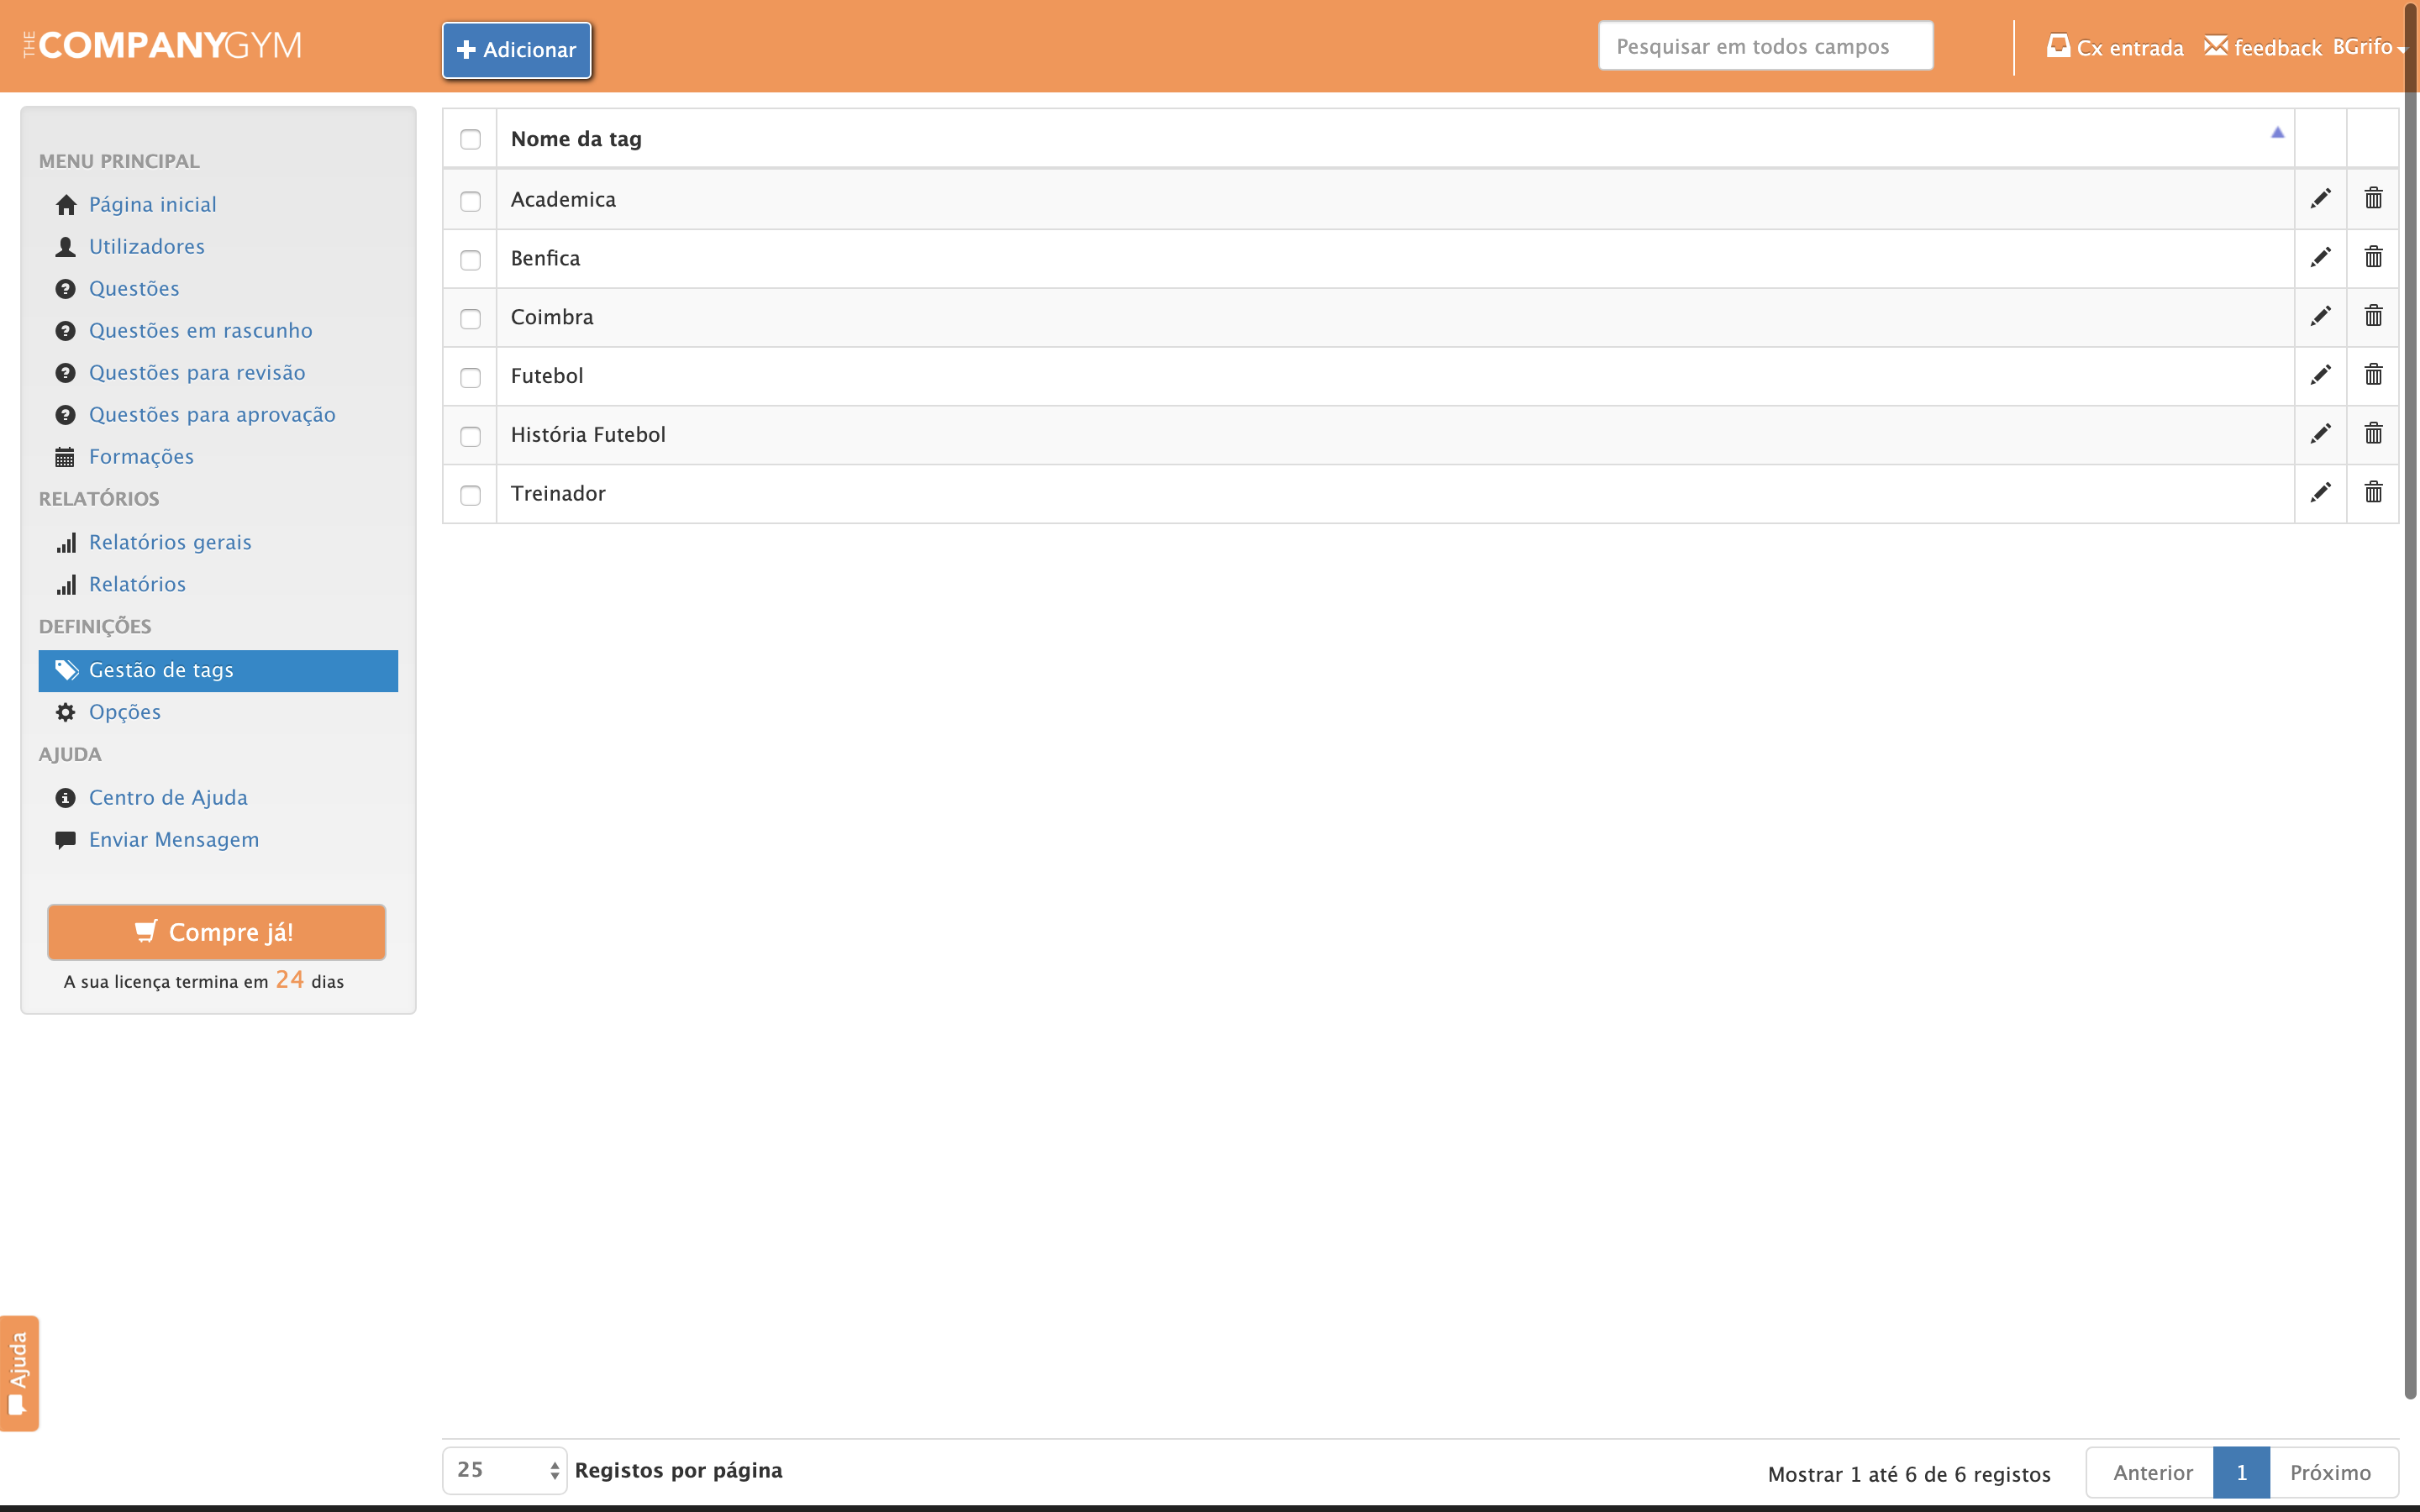
\includegraphics[width=1\textwidth]{img/tcg/tcg-tags.png}
		\caption{The Company Gym - Lista de Tags}
		\label{fig:tcg-tags}
	\end{center}
\end{figure}

É também possivel gerir todas as Tags (i. e. adicionar, editar e remover) adicionadas pelo utilizador no sistema como podemos ver na Figura \ref{fig:tcg-tags} e alterar o template do mail que é enviado para os clientes finais com o link para a formação, representado na Figura \ref{fig:tcg-mail}. 

\begin{figure}[ht!]
	\begin{center}
		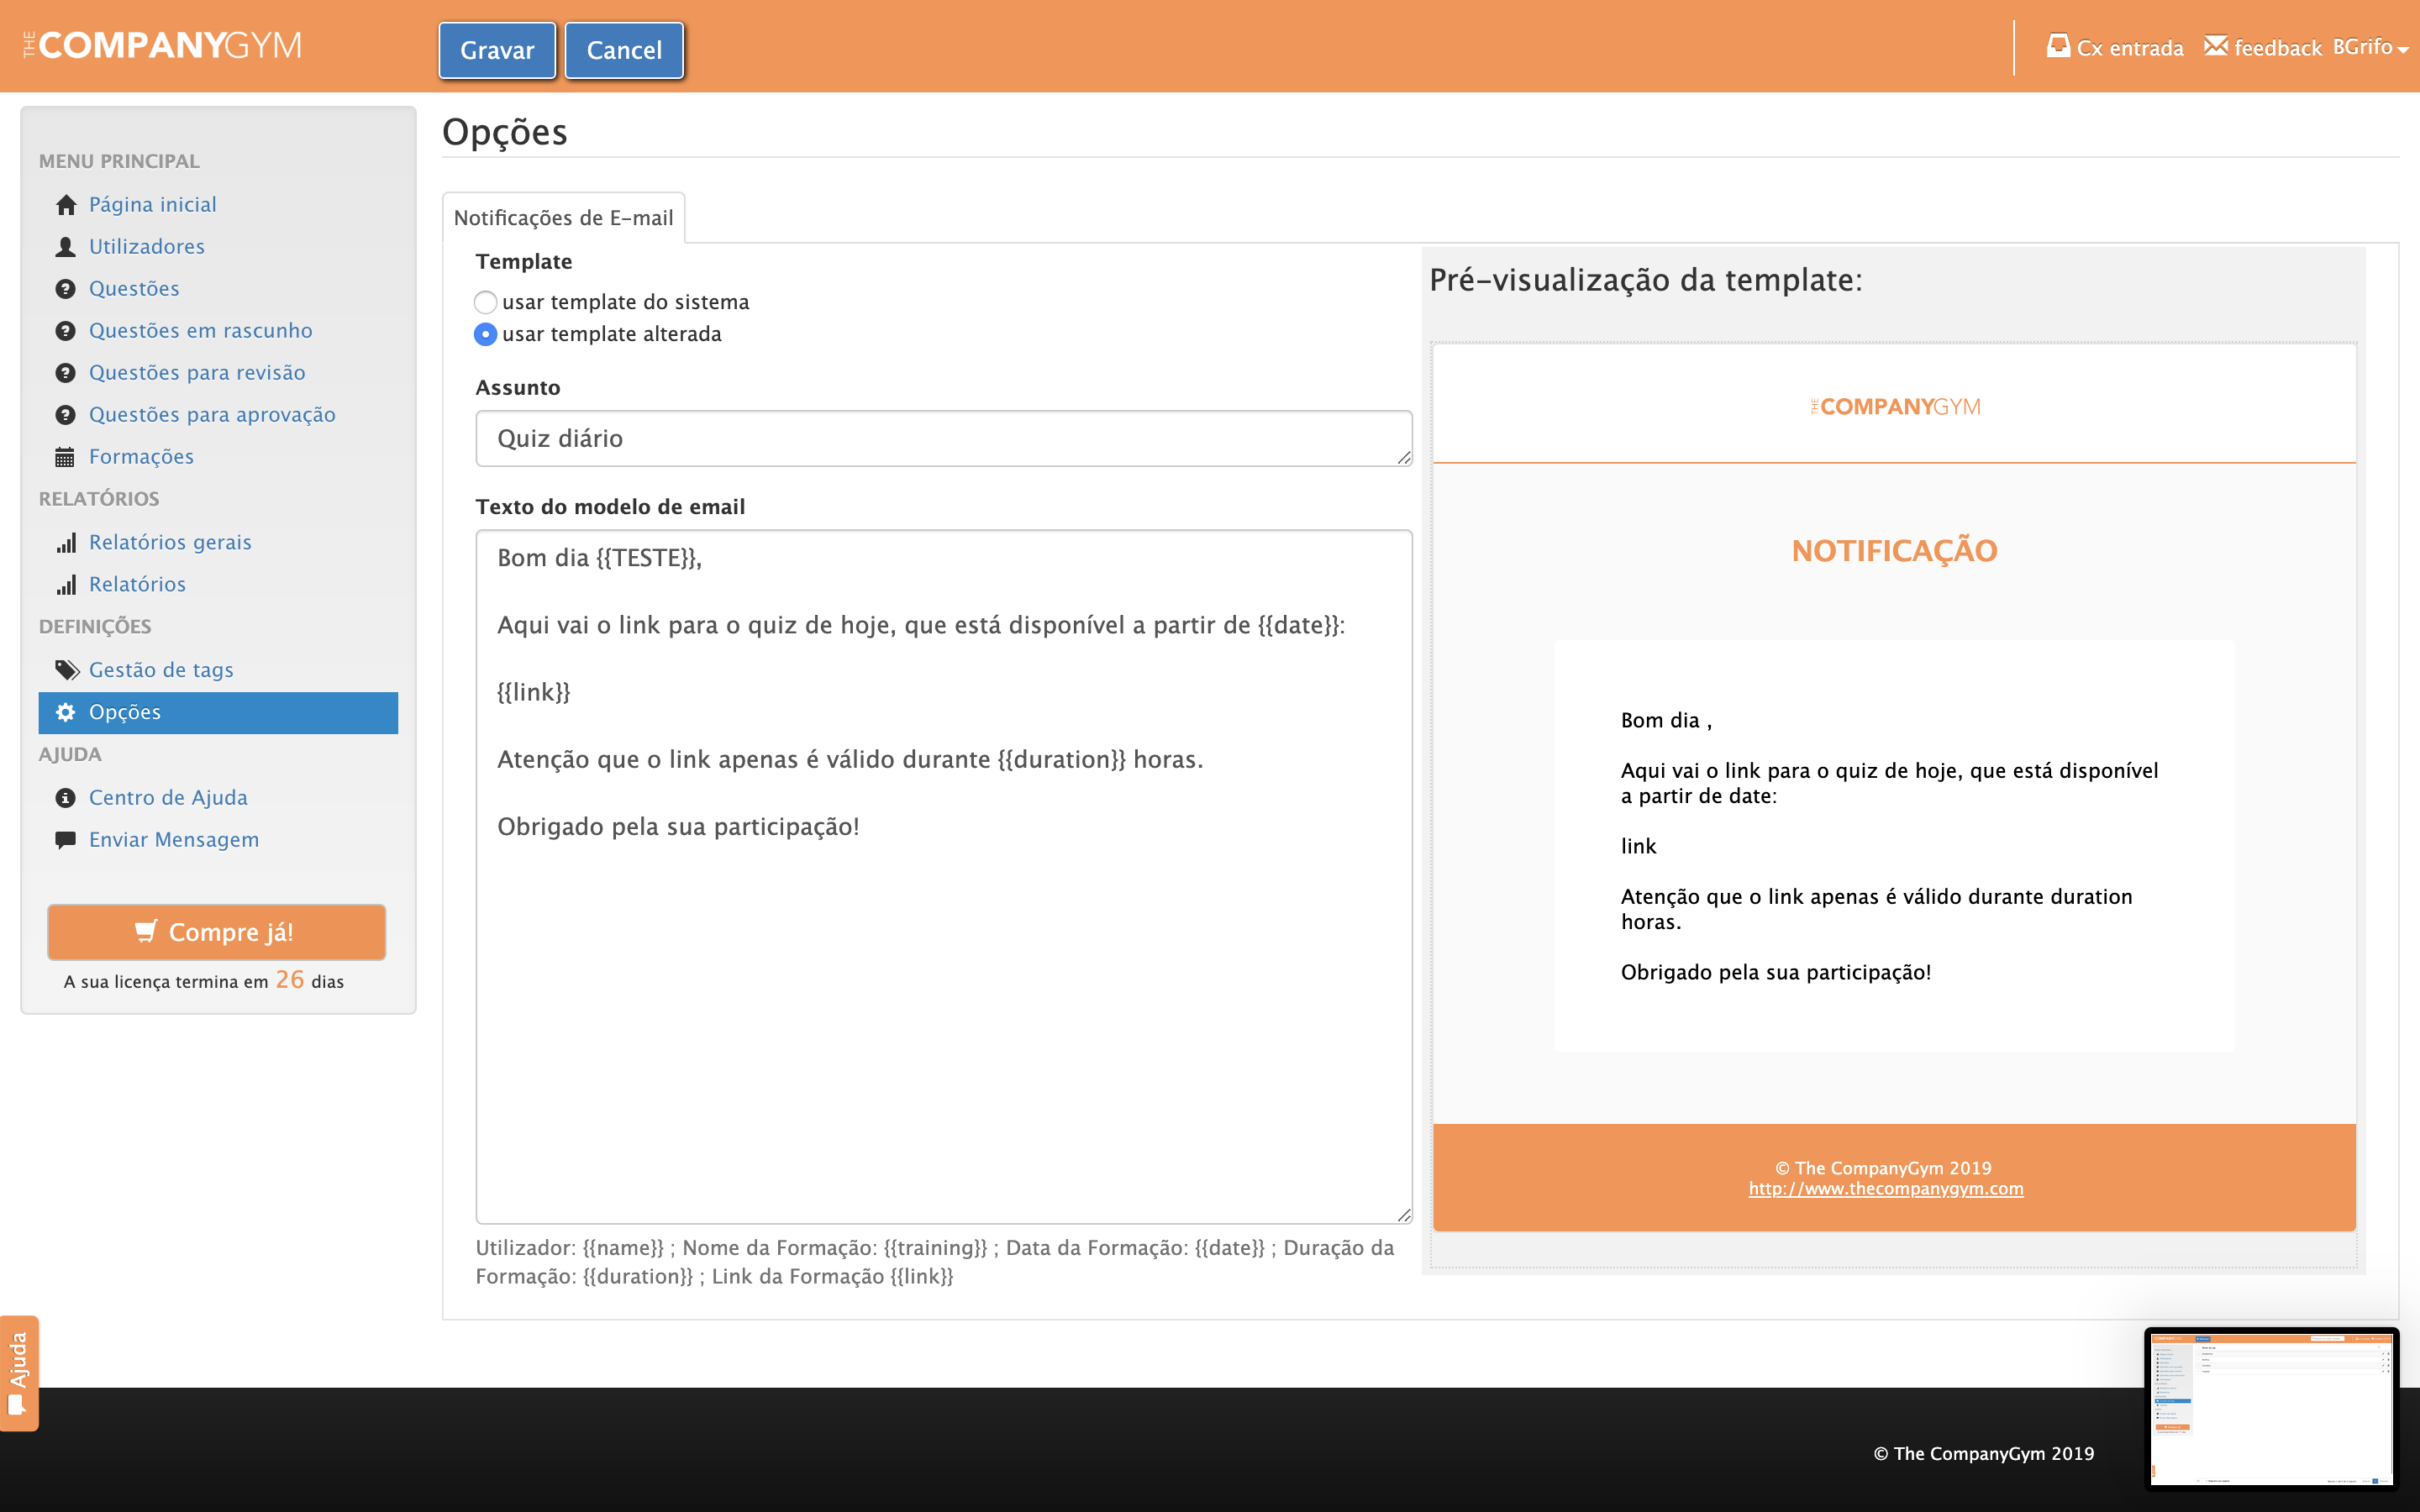
\includegraphics[width=1\textwidth]{img/tcg/tcg-mail.png}
		\caption{The Company Gym - Alterar template do mail}
		\label{fig:tcg-mail}
	\end{center}
\end{figure}

\newpage

Na analise de resultados, podemos gerar relatórios gerais (i. e. relatórios com estatísticas de todas as formações, questões e utilizadores), como podemos ver na Figura \ref{fig:tcg-data}  e relatórios para uma formação em especifico (i. e. relatórios com estatísticas apenas das formações, questões e utilizadores adicionados a essa formação). 

\begin{figure}[ht!]
	\begin{center}
		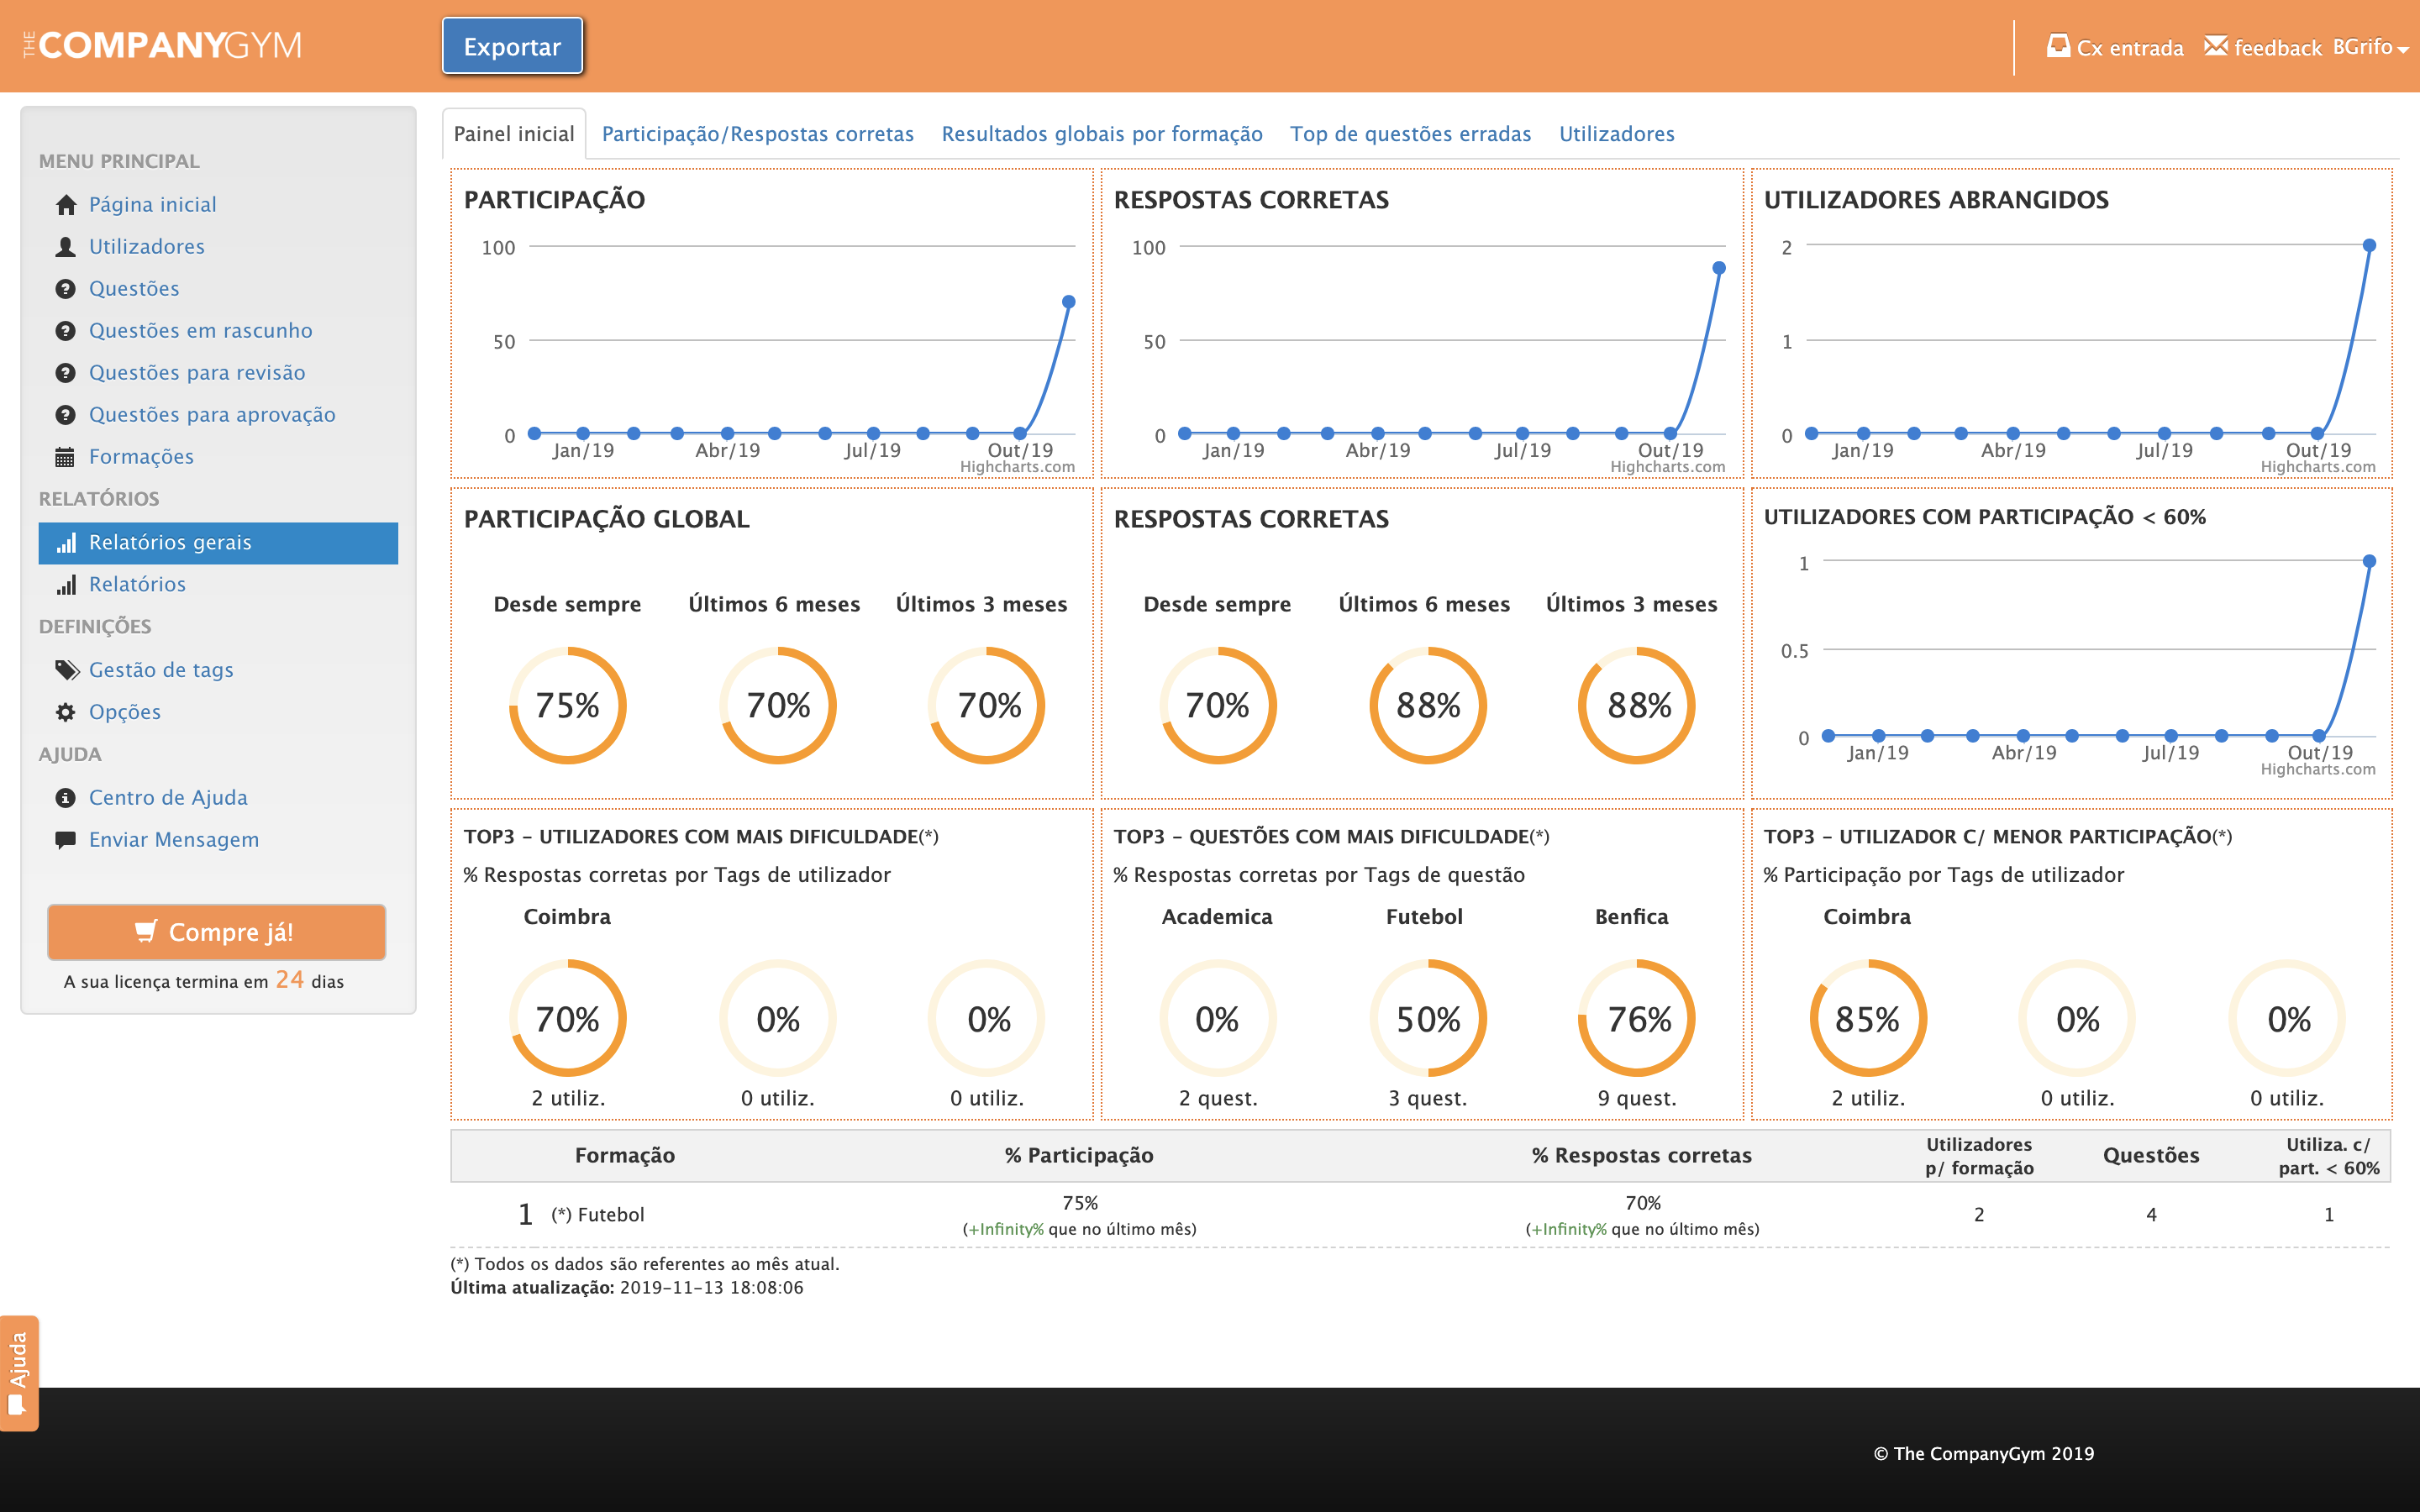
\includegraphics[width=1\textwidth]{img/tcg/tcg-data.png}
		\caption{The Company Gym - Relatório geral (Painel inicial)}
		\label{fig:tcg-data}
	\end{center}
\end{figure}

\newpage

\begin{figure}[ht!]
	\begin{center}
		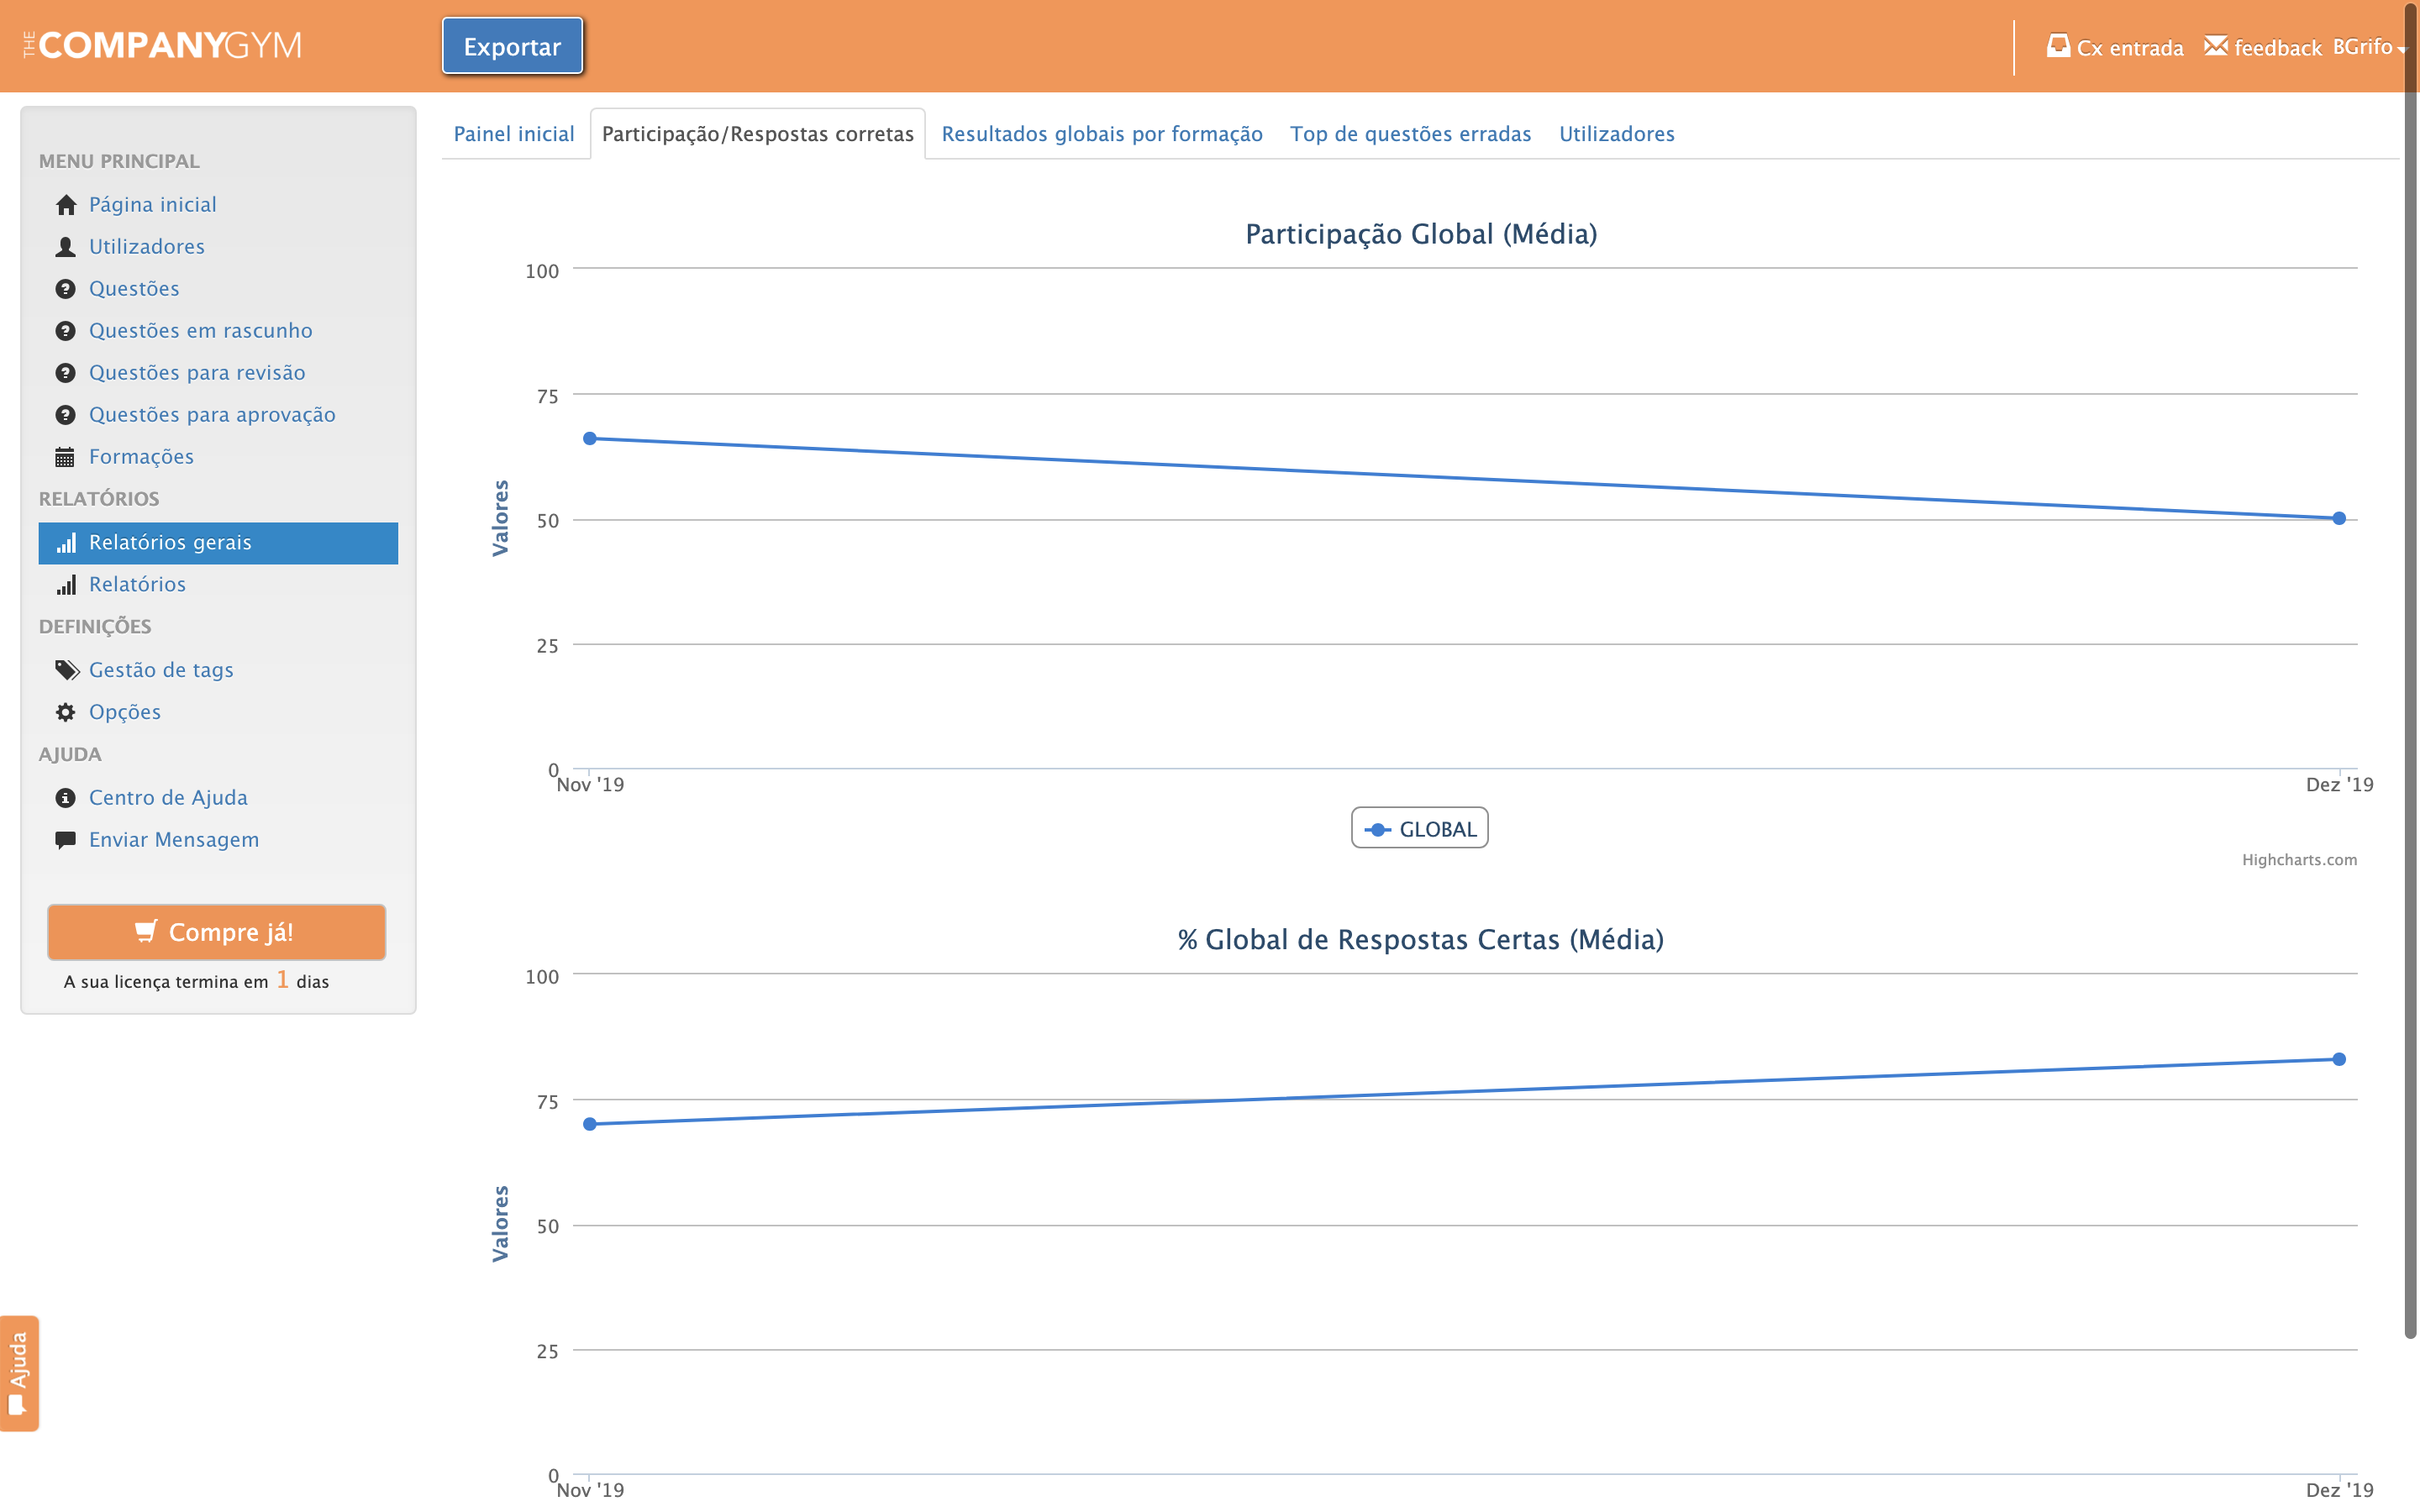
\includegraphics[width=1\textwidth]{img/tcg/tcg-data1.png}
		\caption{The Company Gym - Relatório geral (Participação/Respostas correctas)}
		\label{fig:tcg-data1}
	\end{center}
\end{figure}

Nas Figuras \ref{fig:tcg-data1} e \ref{fig:tcg-data2} temos reprentados a participação/respostas correctas de todas as formações e os resultados globais por formação, respectivamente.

\begin{figure}[ht!]
	\begin{center}
		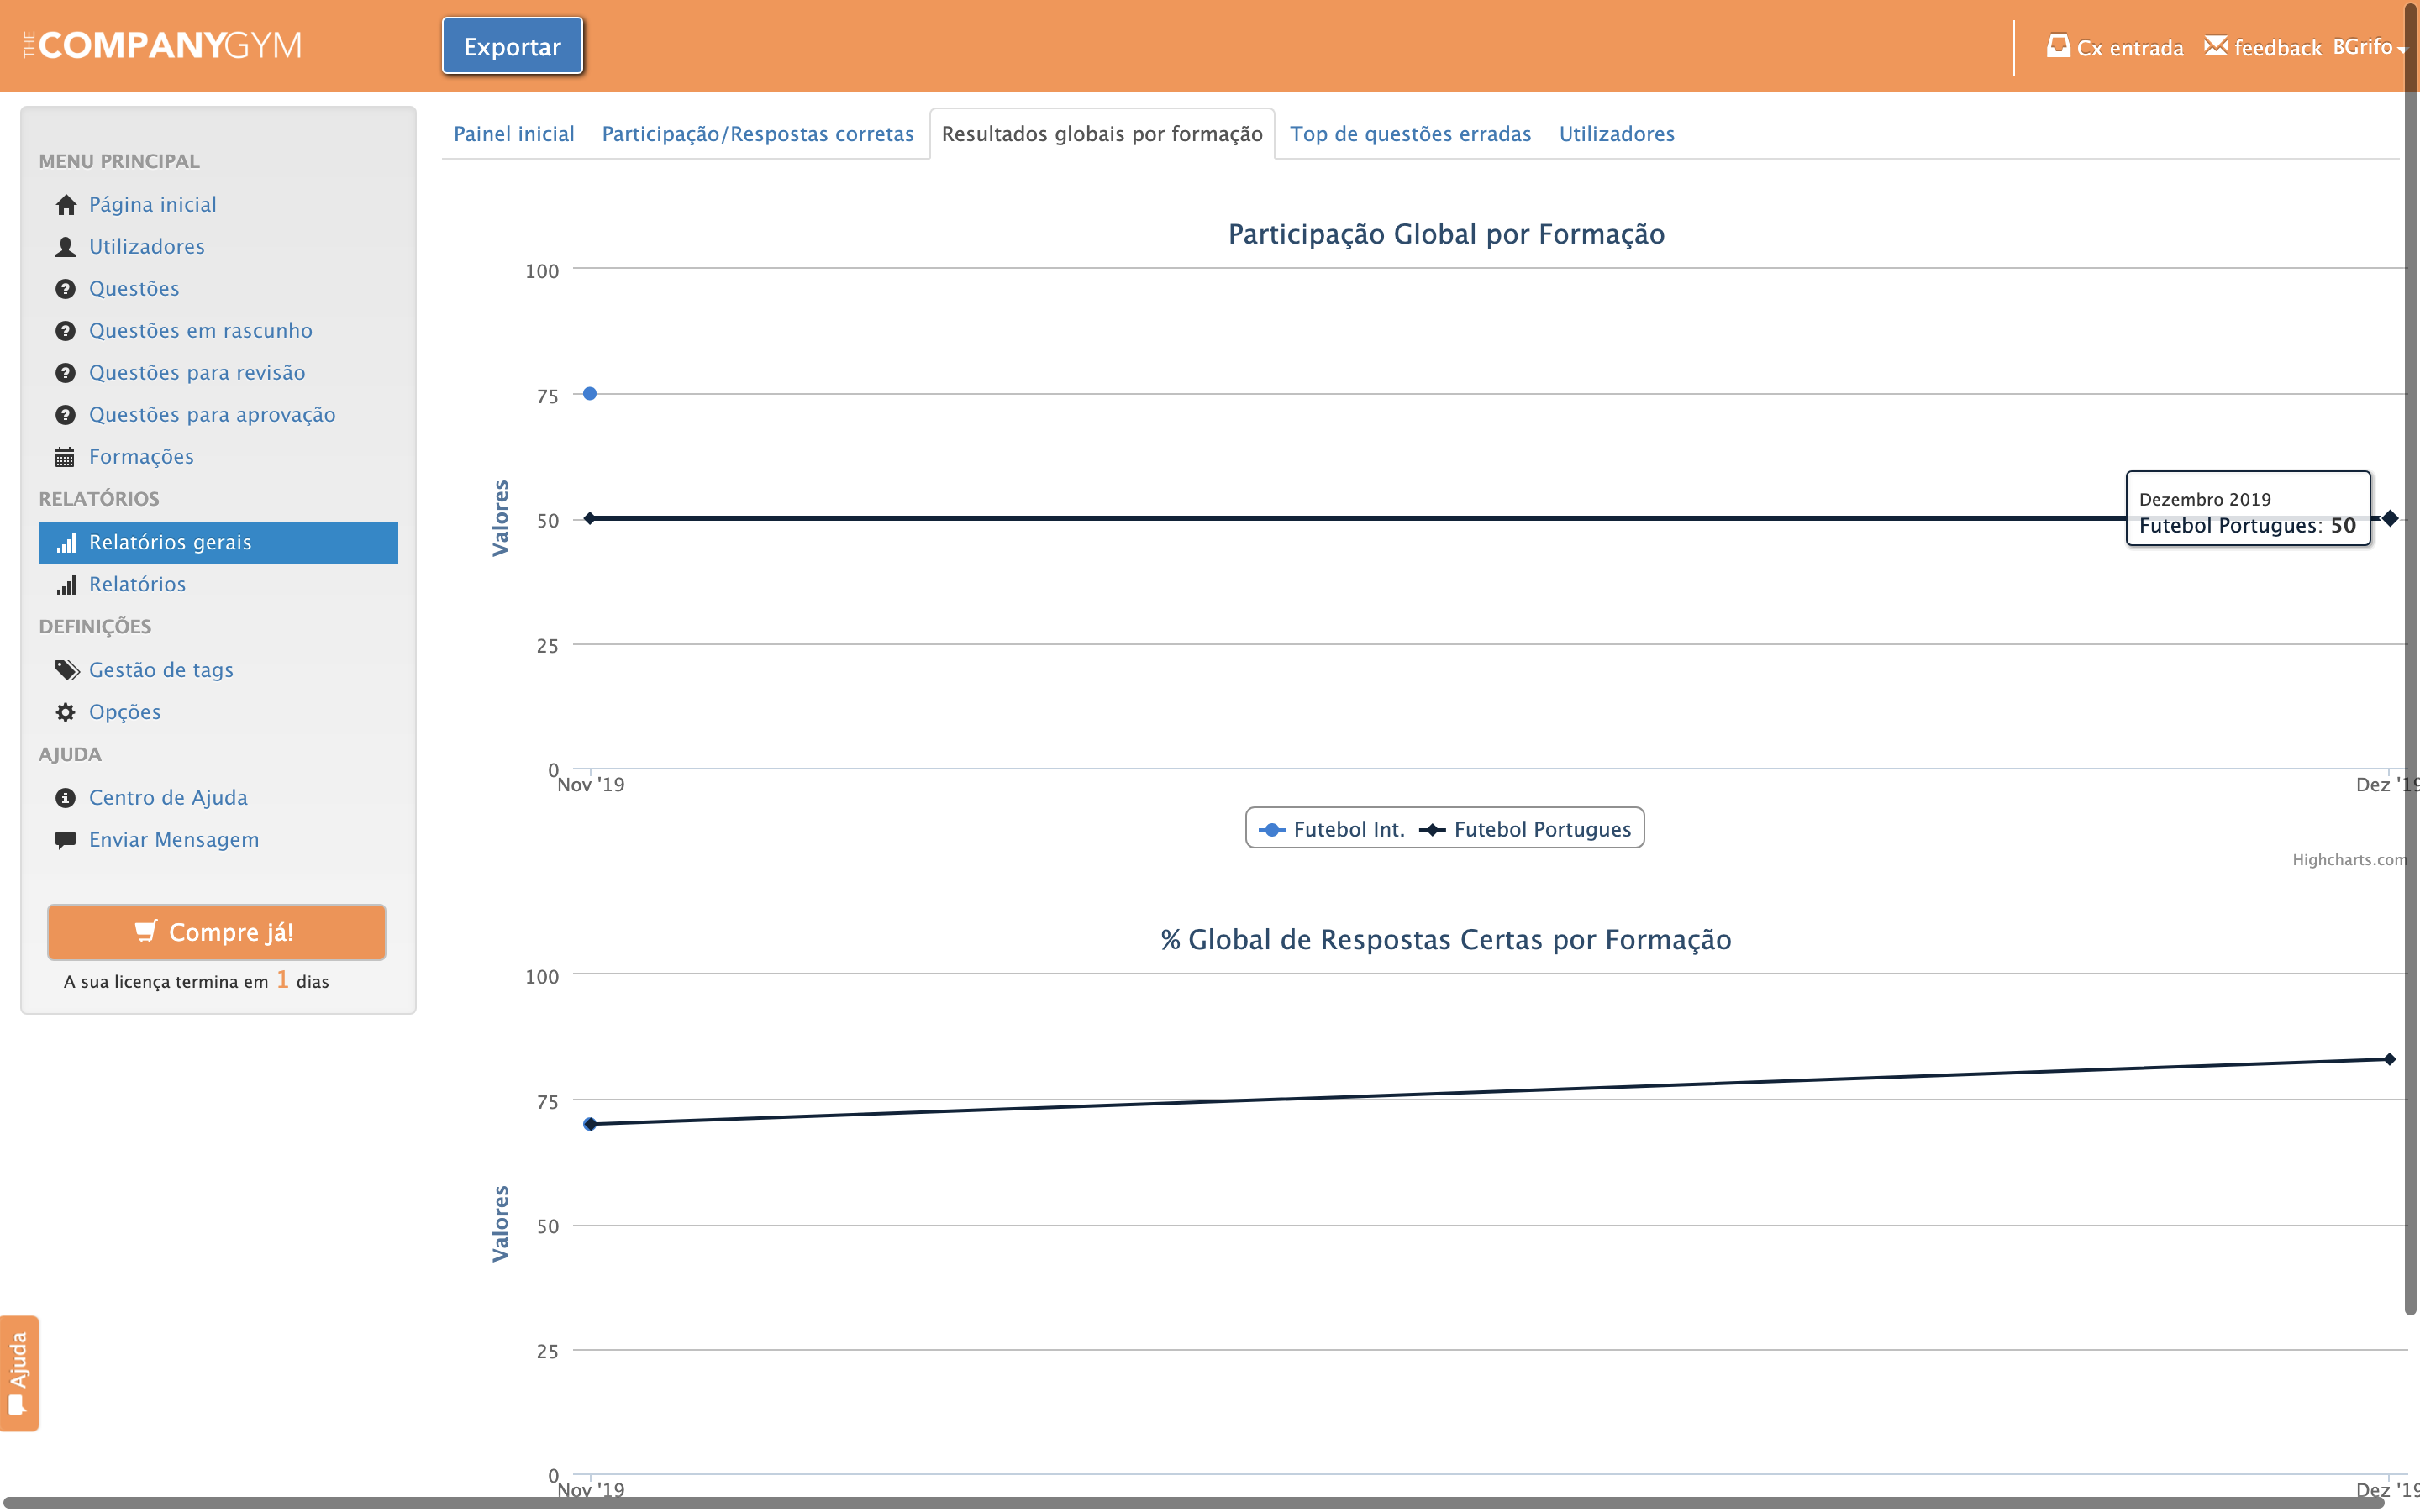
\includegraphics[width=1\textwidth]{img/tcg/tcg-data2.png}
		\caption{The Company Gym - Relatório geral (Resultados globais por formação)}
		\label{fig:tcg-data2}
	\end{center}
\end{figure}

\newpage


No relatório geral é também possível monitorizar quais as questões com maior numero de respostas erradas e o desempenho de cada utilizador final, como podemos ver nas Figuras \ref{fig:tcg-data3} e \ref{fig:tcg-data4}, respectivamente, numa escala temporal definida pelo utilizador. 

\begin{figure}[ht!]
	\begin{center}
		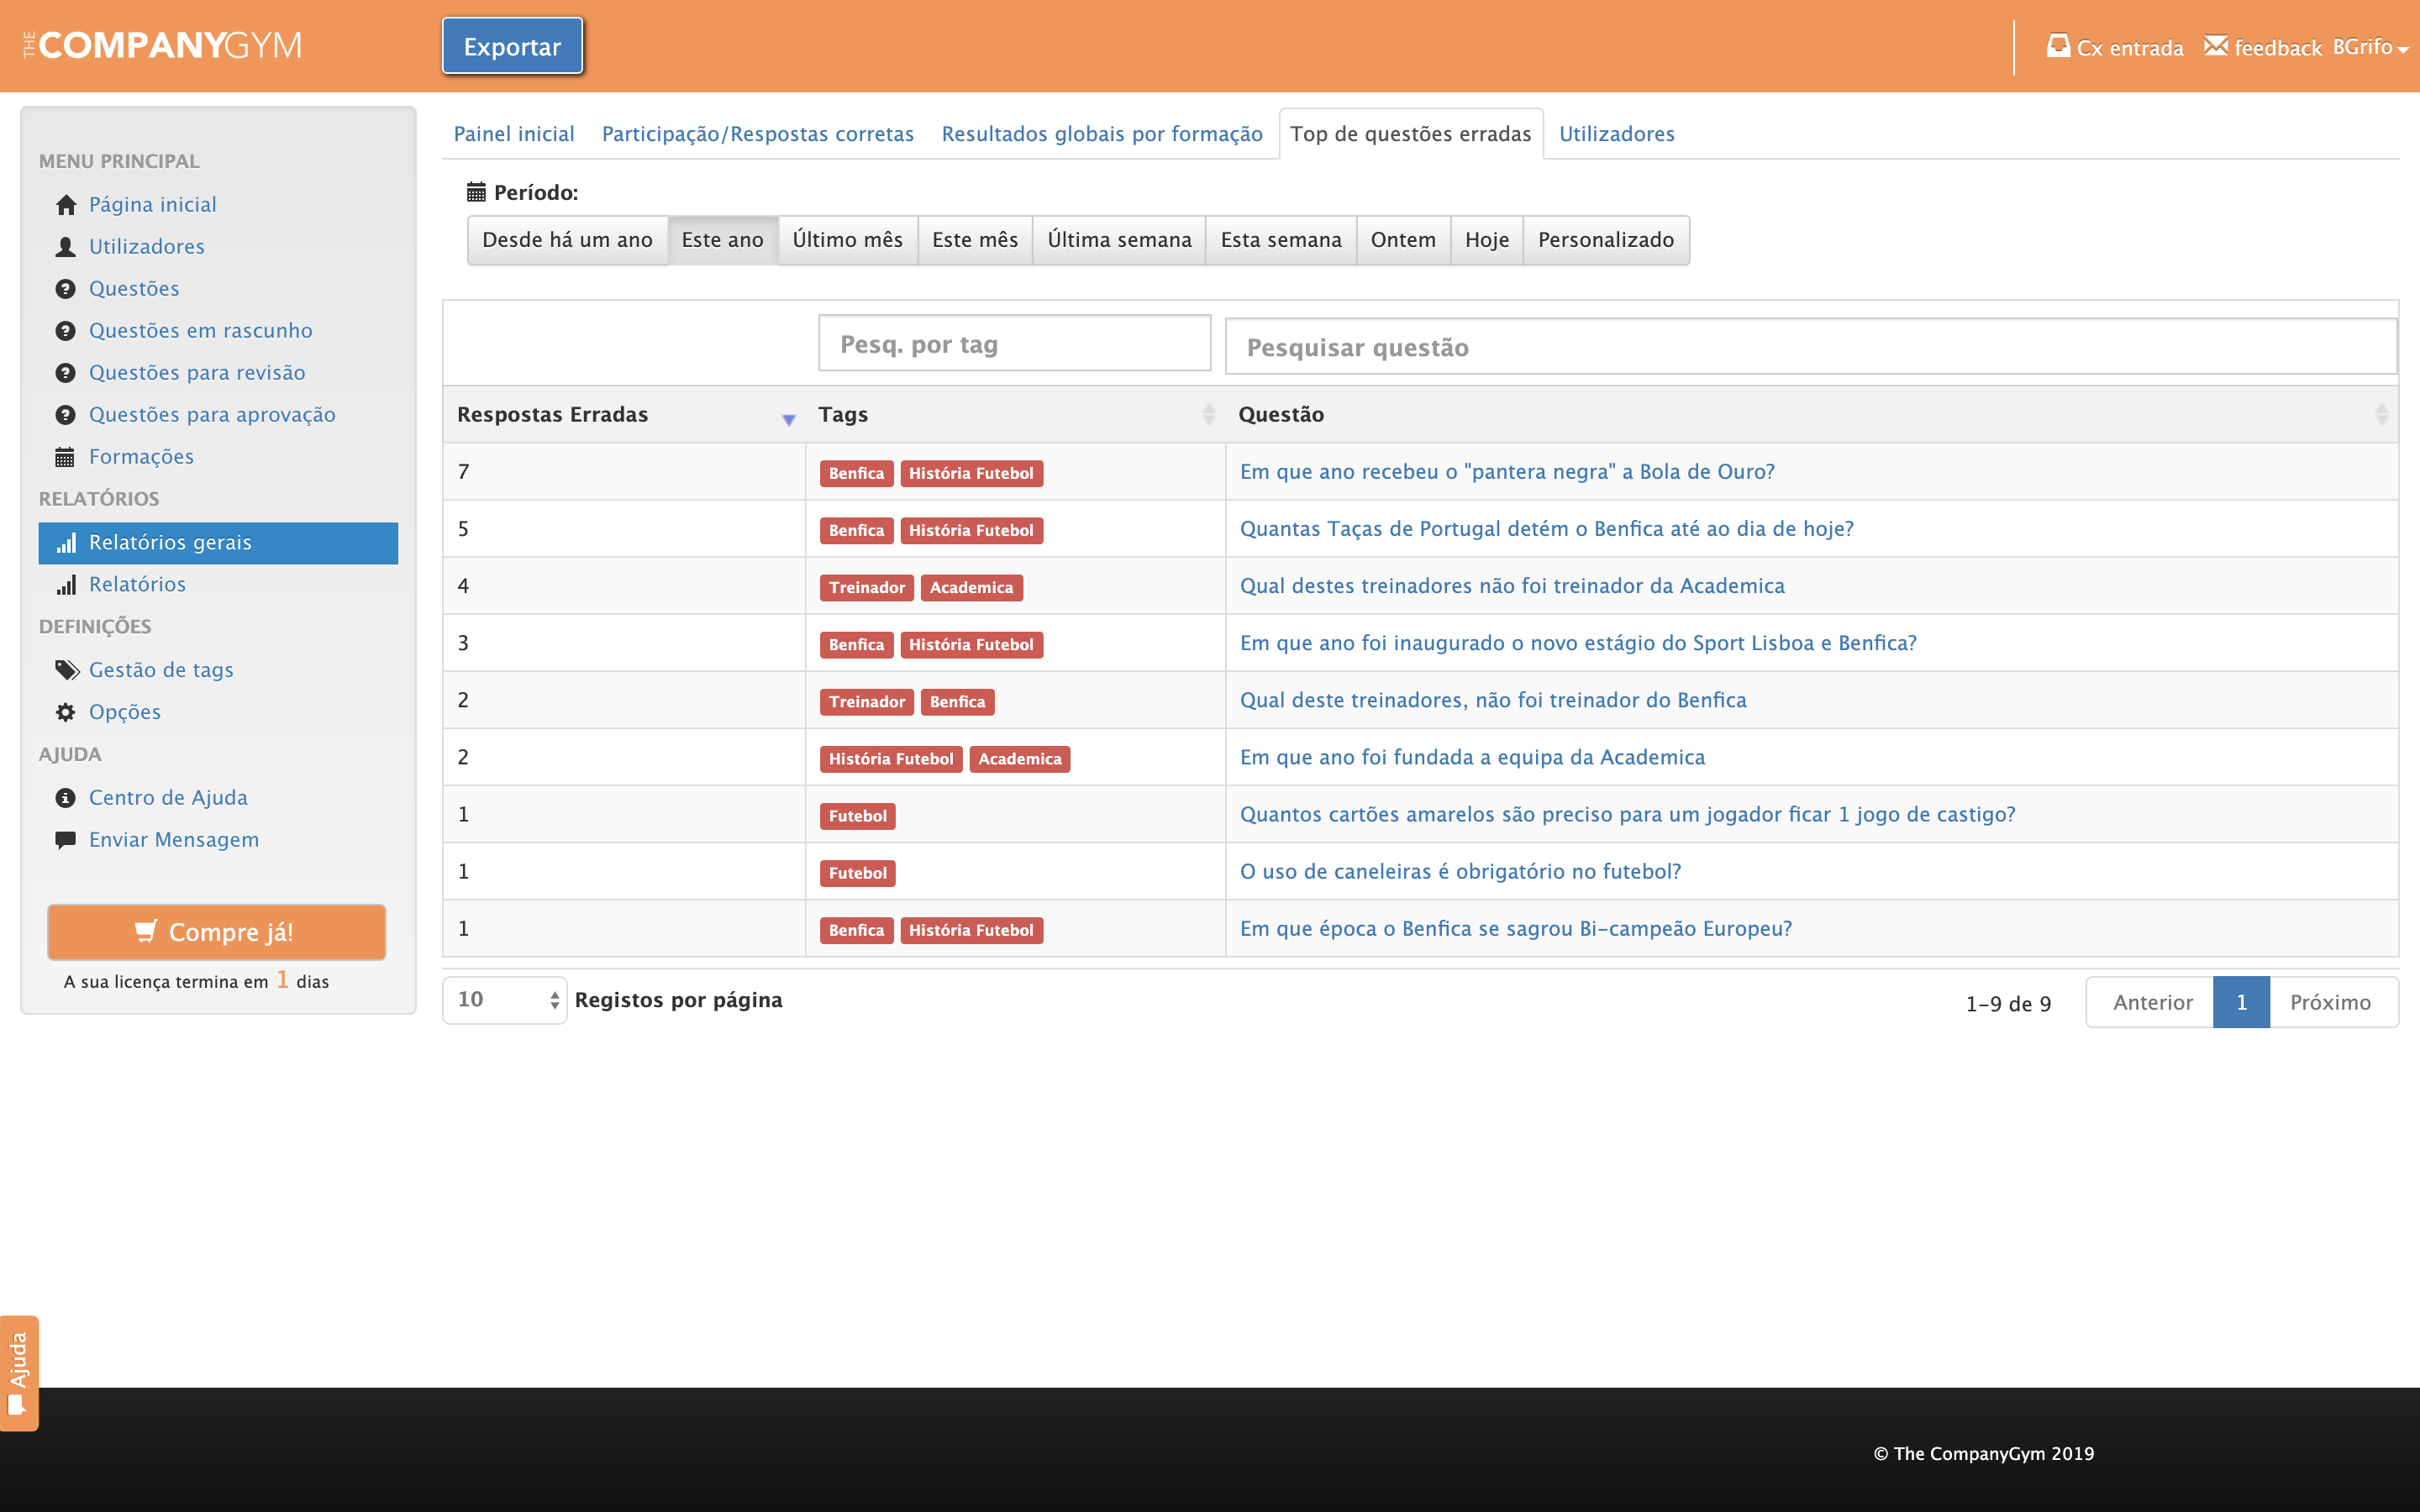
\includegraphics[width=1\textwidth]{img/tcg/tcg-data3.png}
		\caption{The Company Gym - Relatório geral (\textit{Top} de questões erradas)}
		\label{fig:tcg-data3}
	\end{center}
\end{figure}

\begin{figure}[ht!]
	\begin{center}
		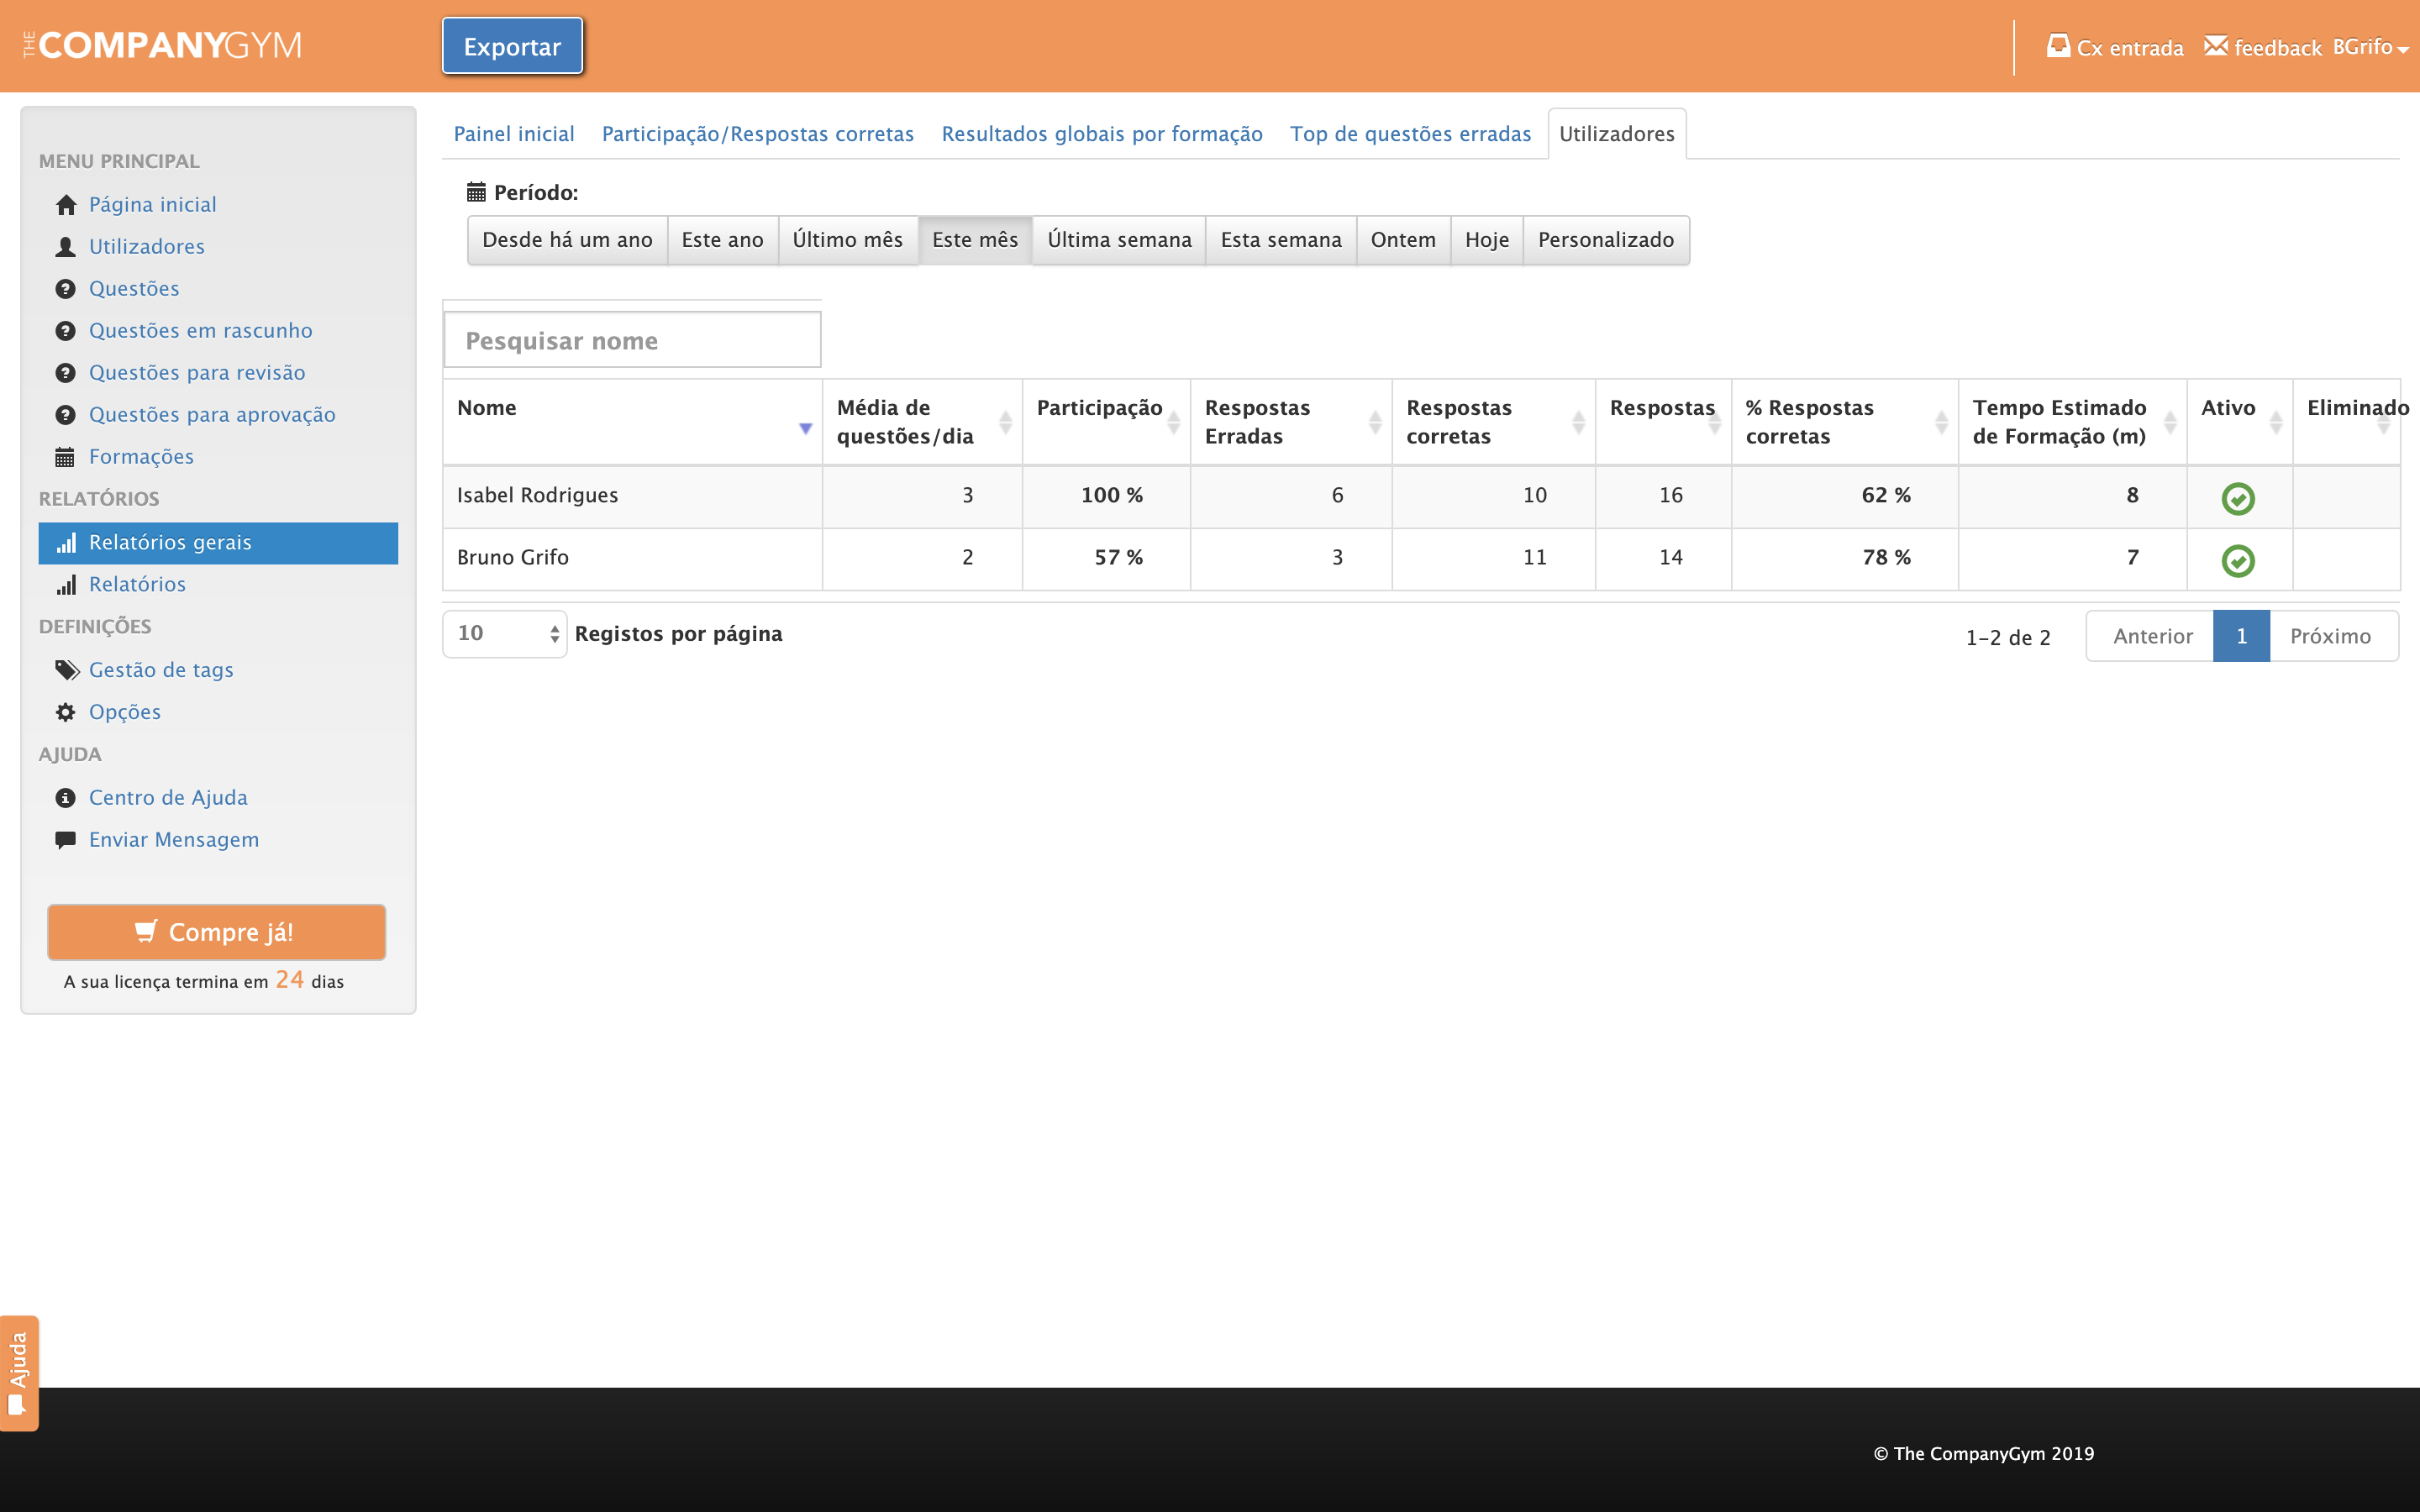
\includegraphics[width=1\textwidth]{img/tcg/tcg-data4.png}
		\caption{The Company Gym - Relatório geral (Utilizadores)}
		\label{fig:tcg-data4}
	\end{center}
\end{figure}

Nos relatórios específicos para uma formação, o tratamento dos dados é muito semelhante como poderemos verificar mais em diante nas Figuras \ref{fig:tcg-data-f},  \ref{fig:tcg-data-f1}, \ref{fig:tcg-data-f2} e \ref{fig:tcg-data-f3}. Depois de selecionar a formação para ser possível gerar o relatório de dados, numa escala temporal definida pelo utilizador, são apresentados os gráficos relativos á percentagem de participação, repostas correctas por \textit{tag} de questão e utilizador. 
No \textit{top} de questões erradas é possível listas os utilizadores finais que erraram uma determinada pergunta. O inverso acontece na página seguinte, representado na Figura \ref{fig:tcg-data-f2}, sendo possível listar as questões onde os utilizadores com mais respostas erradas, erraram. 
Por fim temos a listagem dos utilizadores finais que estão associados à formação em questão, seguidos das estatisticas relacionadas com o seu desempenho.

\begin{figure}[ht!]
	\begin{center}
		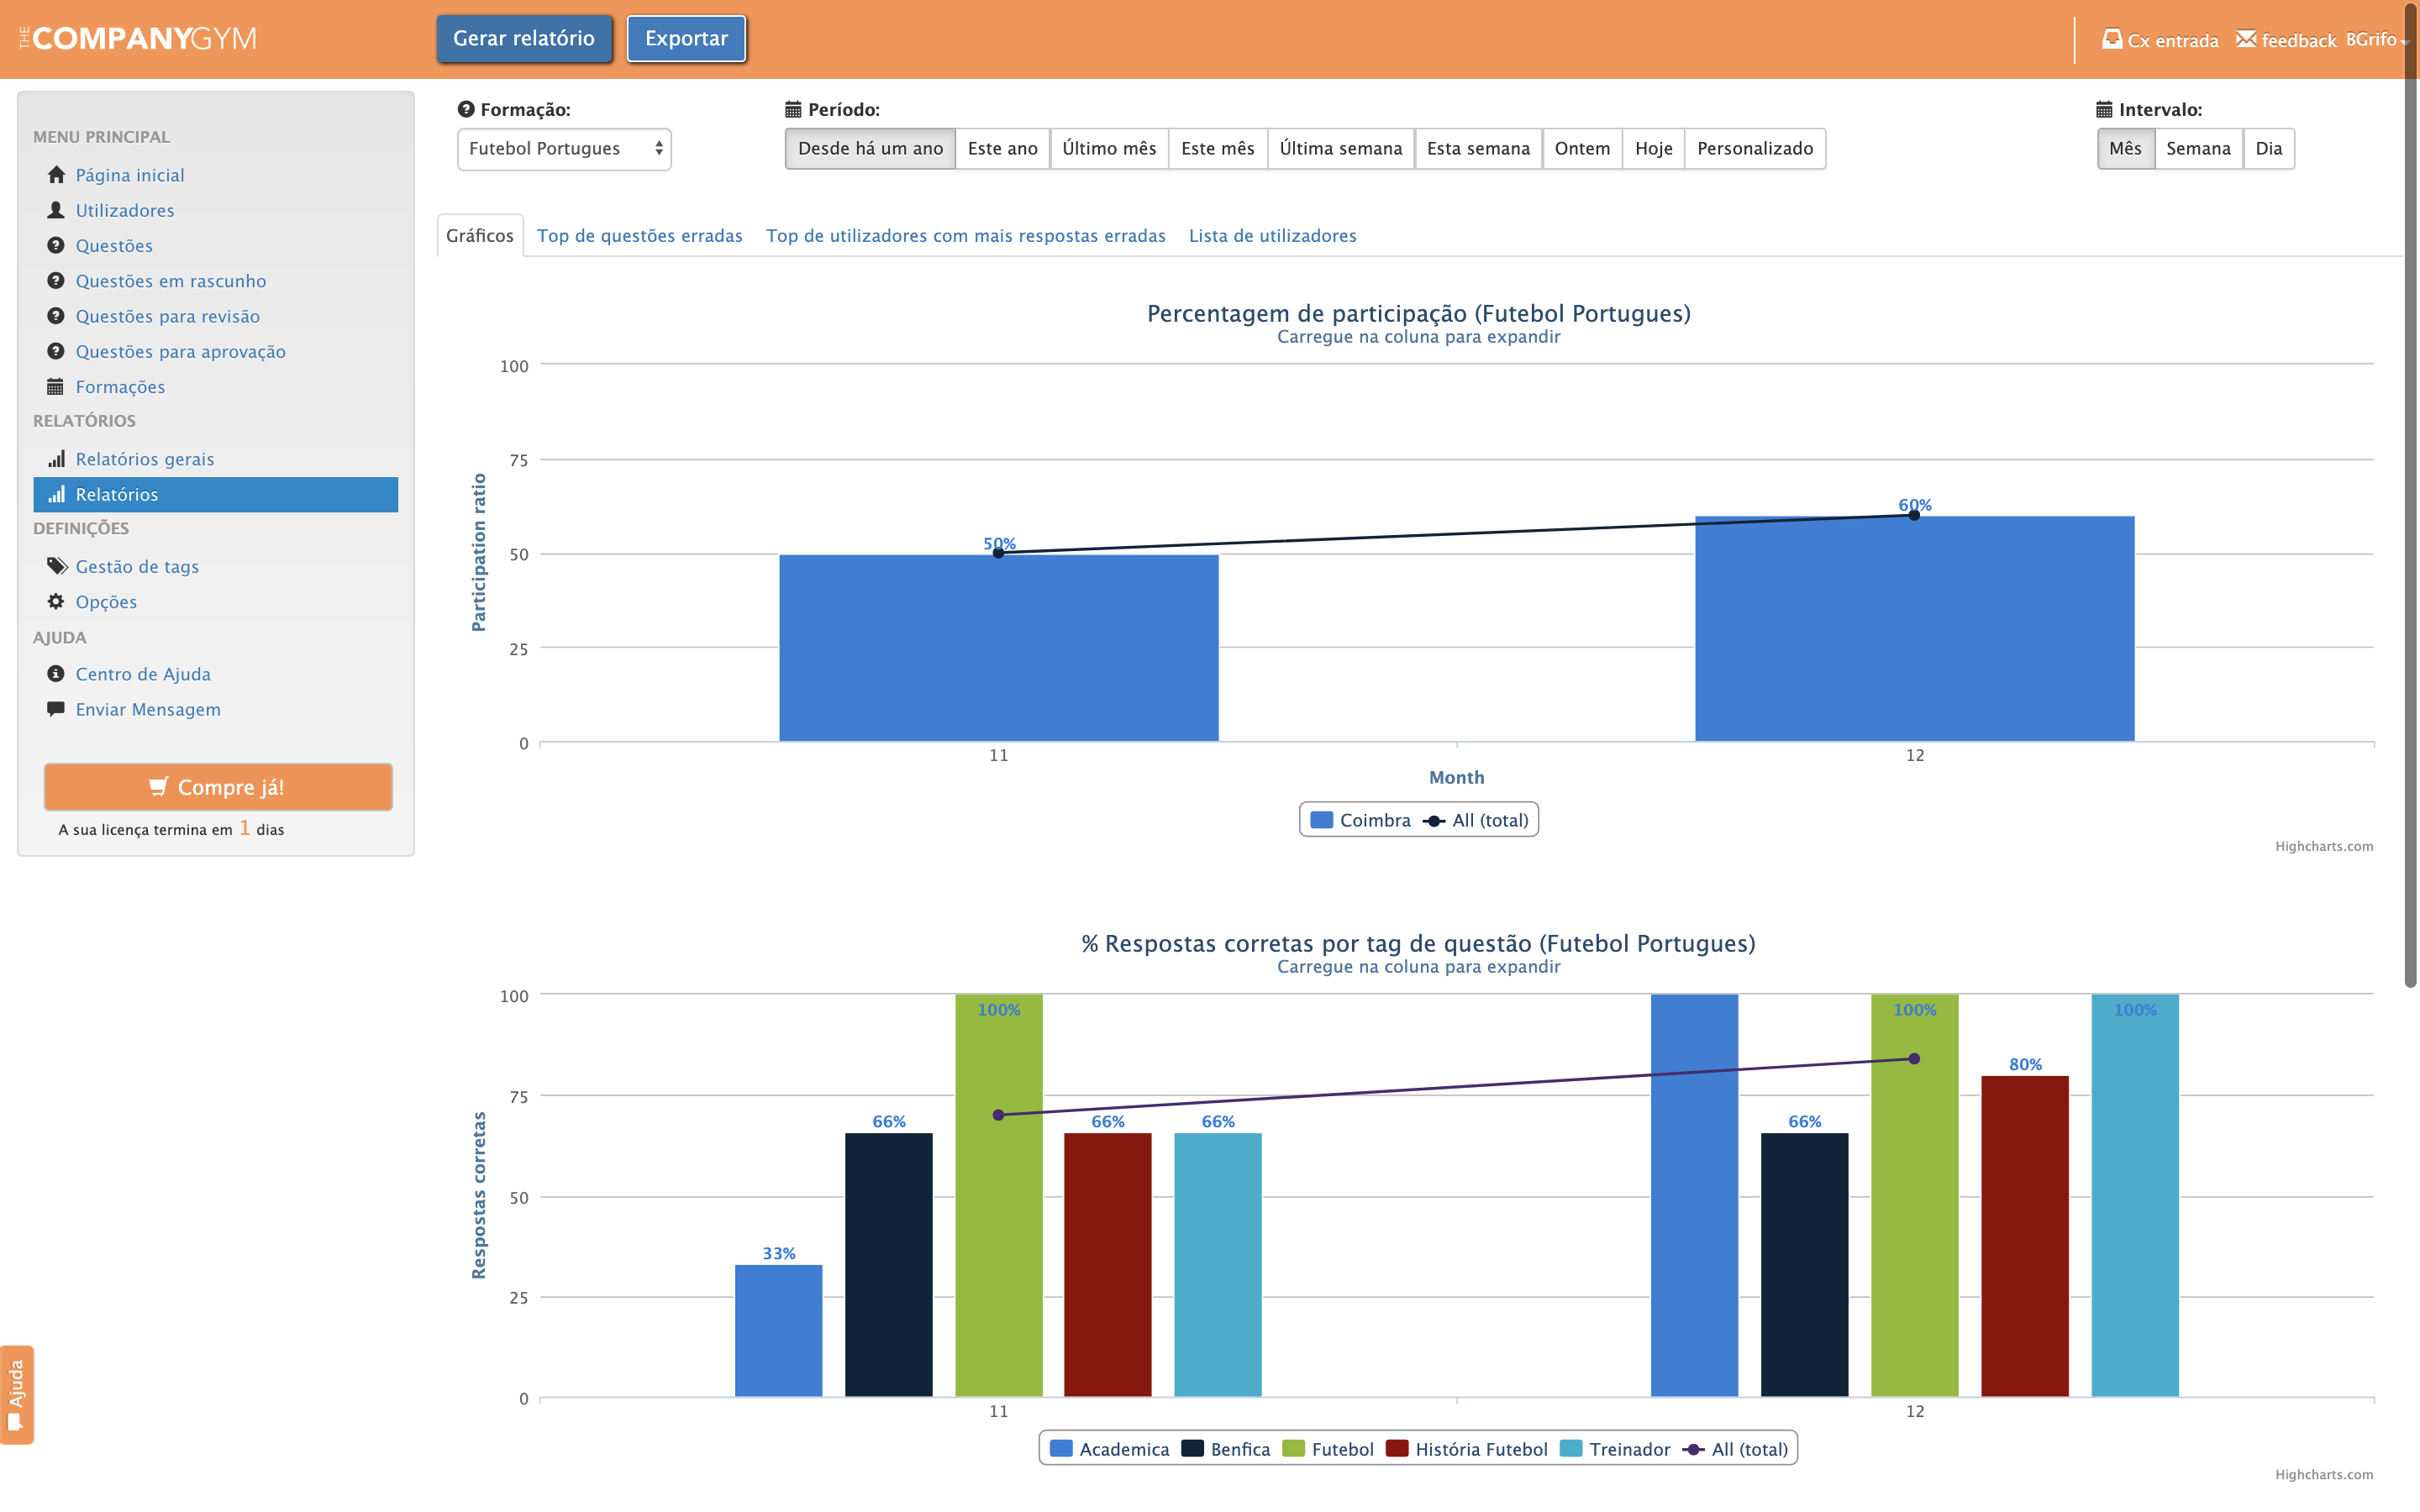
\includegraphics[width=1\textwidth]{img/tcg/tcg-data-f.png}
		\caption{The Company Gym - Relatório específico de uma formação (Gráficos)}
		\label{fig:tcg-data-f}
	\end{center}
\end{figure}

\begin{figure}[ht!]
	\begin{center}
		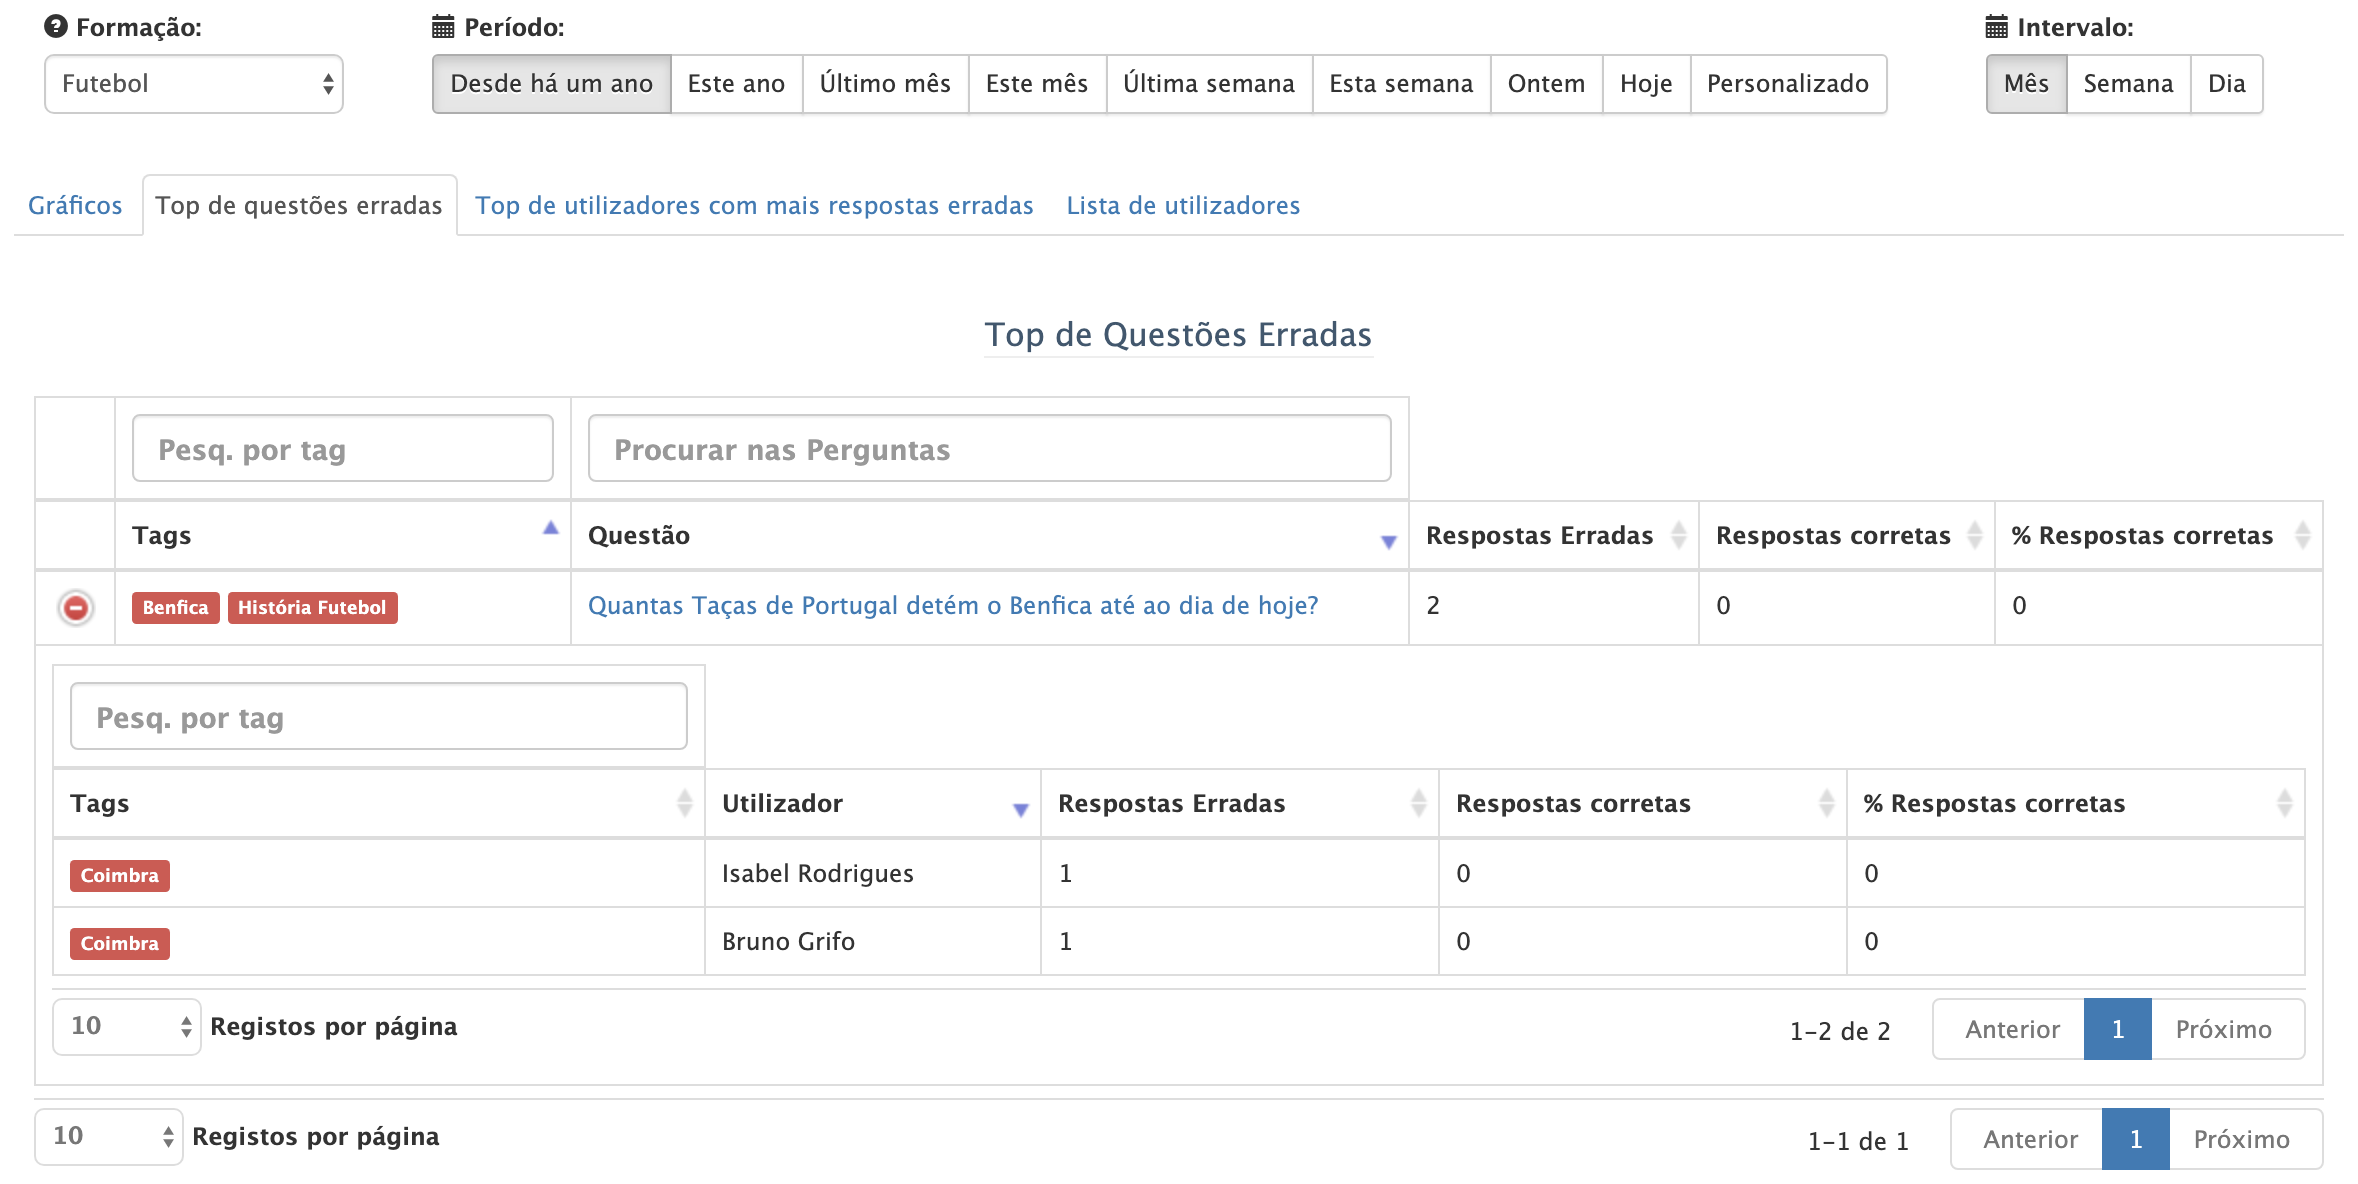
\includegraphics[width=1\textwidth]{img/tcg/tcg-data-f1.png}
		\caption{The Company Gym - Relatório específico de uma formação (\textit{Top} de questões erradas)}
		\label{fig:tcg-data-f1}
	\end{center}
\end{figure}
\mbox{}
\begin{figure}[ht!]
	\begin{center}
		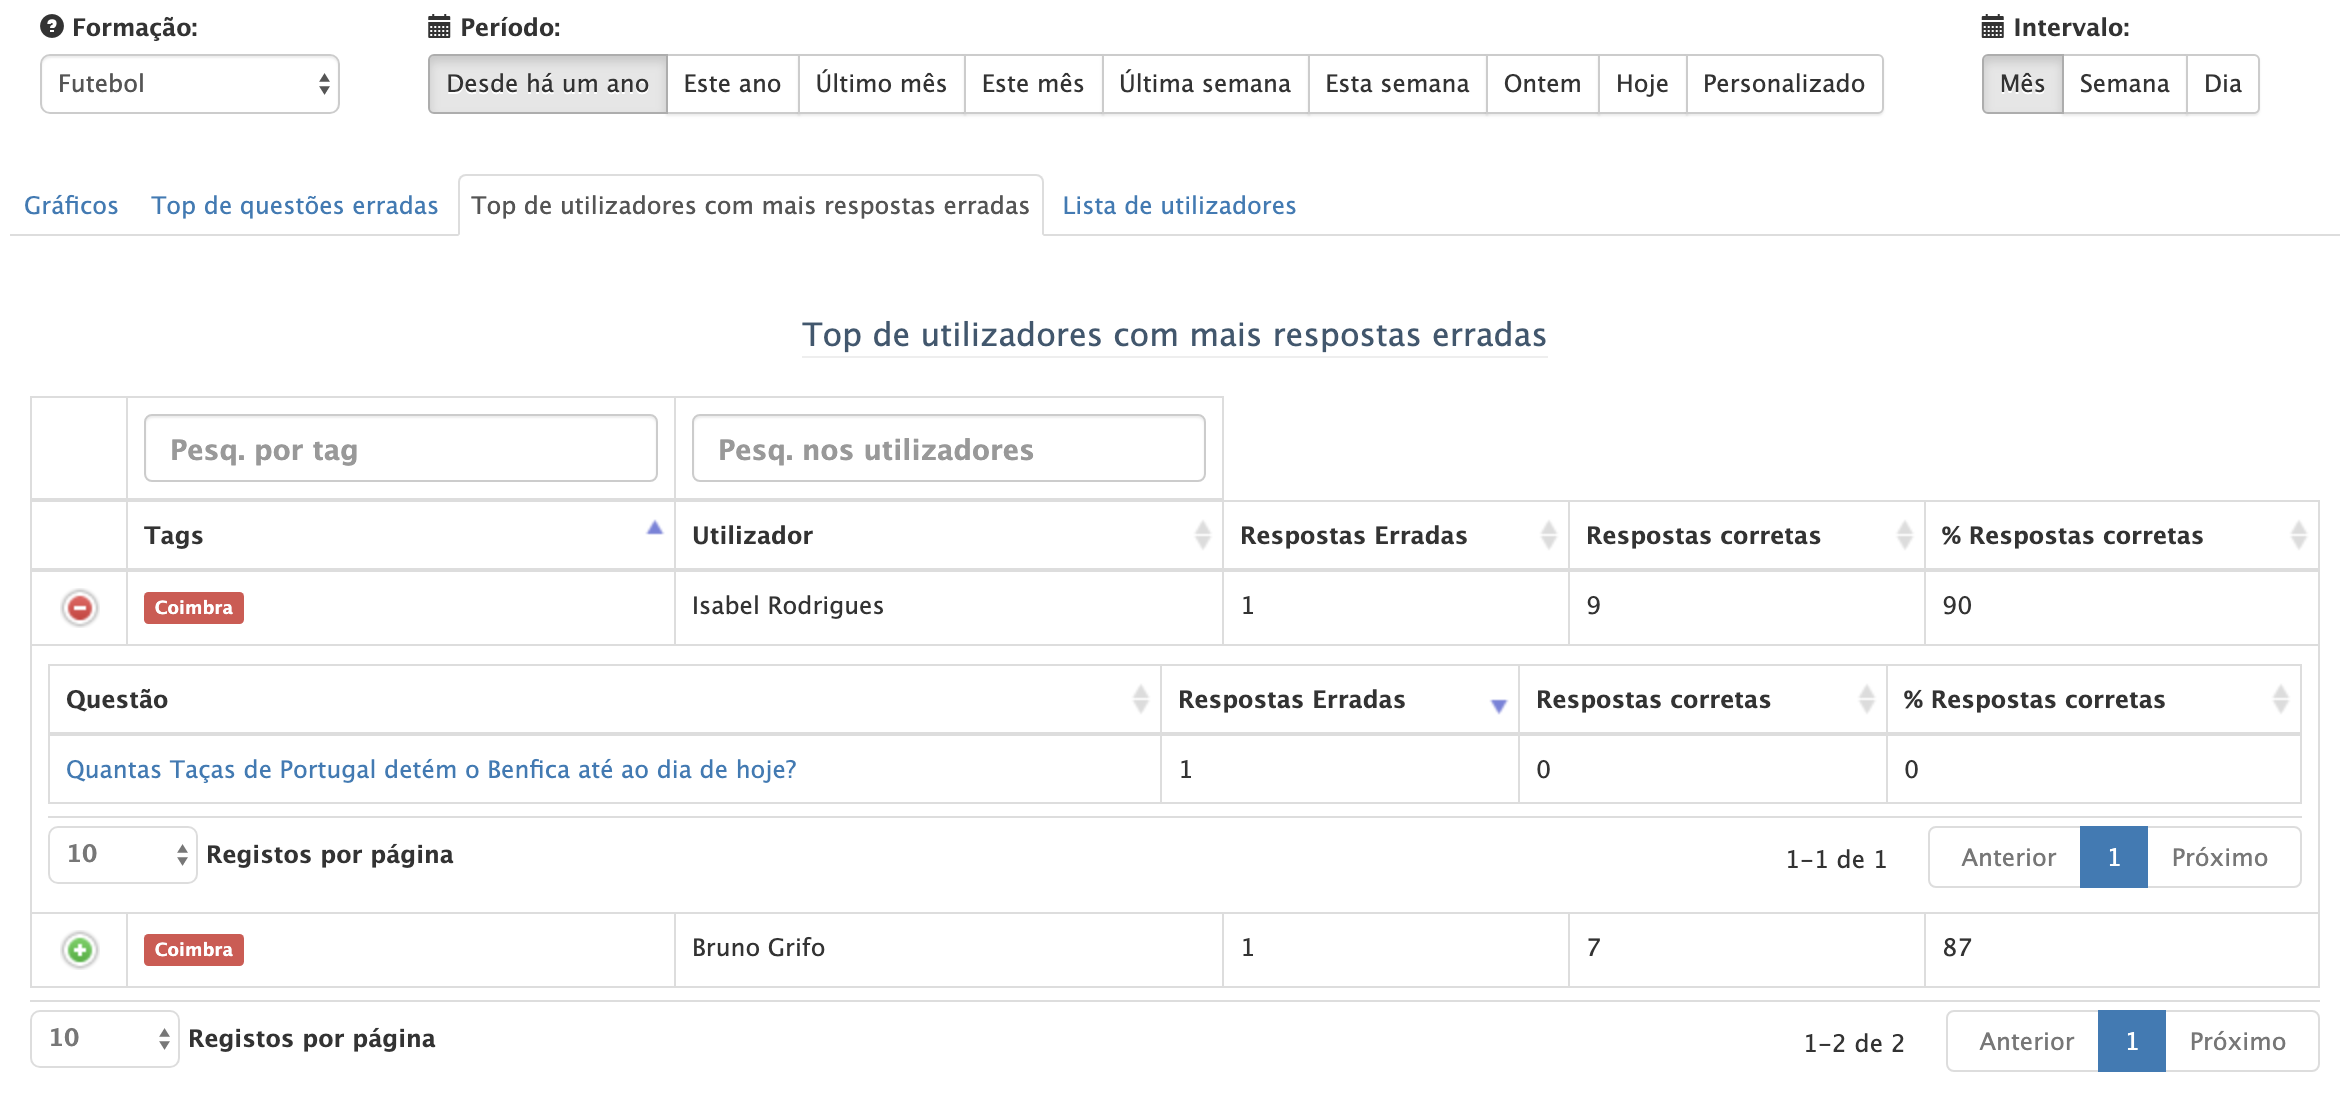
\includegraphics[width=1\textwidth]{img/tcg/tcg-data-f2.png}
		\caption{The Company Gym - Relatório específico de uma formação (\textit{Top} de utilizadores com mais respostas erradas)}
		\label{fig:tcg-data-f2}
	\end{center}
\end{figure}

\begin{figure}[ht!]
	\begin{center}
		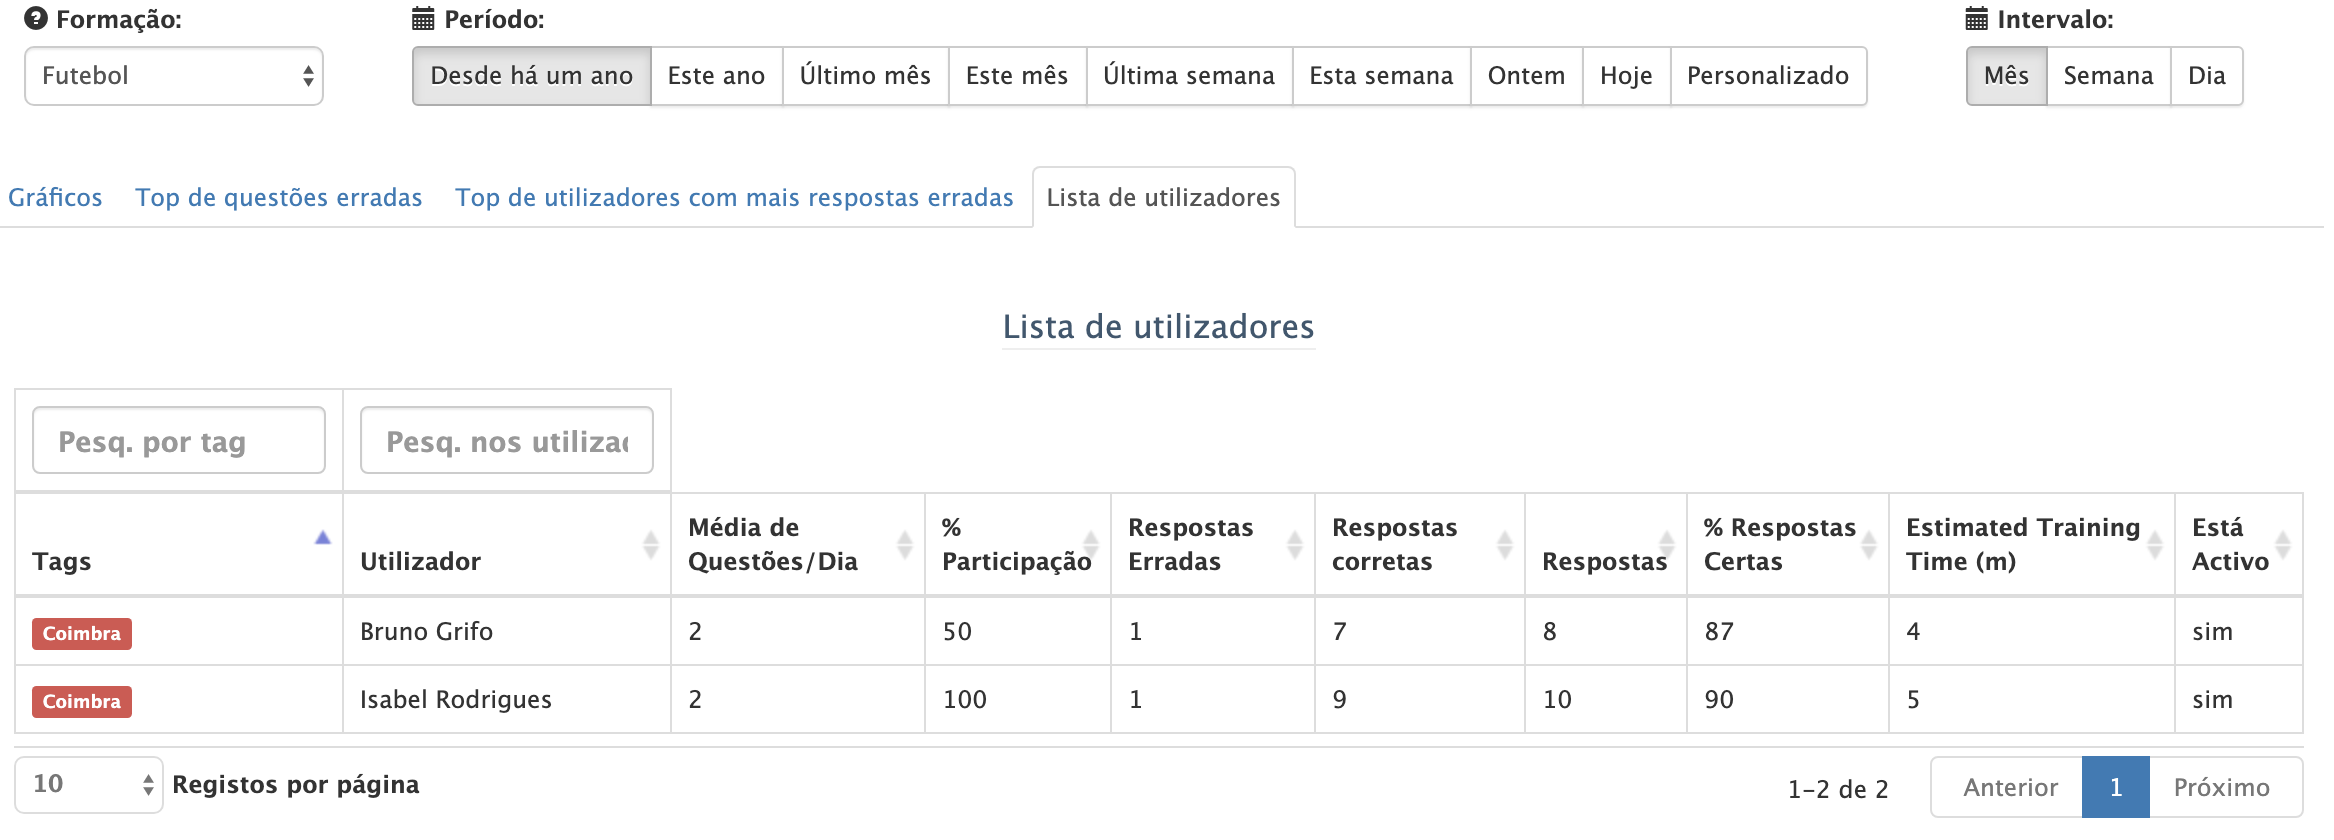
\includegraphics[width=1\textwidth]{img/tcg/tcg-data-f3.png}
		\caption{The Company Gym - Relatório específico de uma formação (Lista de utilizadores)}
		\label{fig:tcg-data-f3}
	\end{center}
\end{figure}

\section{\acrfull{ex.co} Platform}
\label{exco}

O \acrshort{ex.co}, anteriormente Playbuzz, é uma plataforma para criação de conteúdo atraente que permite recolher informação do público alvo através de experiências. Esta plataforma permite também a analise da informação recolhida ajudando a perceber as novas \gls{lead}.

Uma das funcionalidades interessantes do \acrshort{ex.co} é a criação de questionários que por exemplo, consoante as respostas do utilizador final, o resultado vai ser diferente, tal como podemos ver nas Figuras \ref{fig:exco-example} e \ref{fig:exco-example3}.


\begin{figure}[ht!]
	\begin{center}
		\includegraphics[width=1\textwidth]{img/exco/example}
		\caption{EX.CO - Exemplo de um Questionário}
		\label{fig:exco-example}
	\end{center}
\end{figure}

\begin{figure}[ht!]
	\begin{center}
		\includegraphics[width=1\textwidth]{img/exco/example3}
		\caption{EX.CO - Resultado do Questionário da Figura \ref{fig:exco-example}}
		\label{fig:exco-example3}
	\end{center}
\end{figure}

\mbox{}
\newpage

O \acrshort{ex.co} não tem nenhum pacote gratuito contudo, fornece um \textit{trial} de 14 dias com acesso à maioria das funcionalidades. Para aceder às funcionalidades da plataforma é necessário a autenticação do utilizador que pode ser por credências ou pelas \acrshort{api}s do Facebook e da Google.

Como podemos ver na Figura \ref{fig:exco-template}, a partir da página inicial temos acesso a templates de experiencias/\textit{items} (i. e. questionários etc..), definições e plano do utilizador, todas as experiencias criadas e respectiva analise. A partir da página principal conseguimos também criar um novo \textit{item} como podemos ver na Figura \ref{fig:exco-new}.

\begin{figure}[ht!]
	\begin{center}
		\includegraphics[width=1\textwidth]{img/exco/templates}
		\caption{EX.CO - Página Inicial}
		\label{fig:exco-template}
	\end{center}
\end{figure}

\begin{figure}[ht!]
	\begin{center}
		\includegraphics[width=1\textwidth]{img/exco/new}
		\caption{EX.CO - Nova experiência}
		\label{fig:exco-new}
	\end{center}
\end{figure}

\newpage

Representado na Figura \ref{fig:exco-pers} temos o inicio do processo da criação de um \textit{quiz} de personalidade. Outras experiências podem ser criadas como podemos observar na Figura anterior, contudo vamos apenas analisar as funcionalidades chaves que competem com o 10.quest.

O primeiro passo a realizar será introduzir resultados em formato de texte. Os resultados podem ser complementados com anexos que, como podemos ver na Figura \ref{fig:exco-img}, podem ser imagens, gifs, vídeos ou emojis da \acrfull{web} ou do dispositivo pessoal.

Para testar as funcionalidades desta ferramenta, foi criado um questionário para calcular o local ideal para passar férias consoante as preferências do utilizador final. Os resultados adicionados foram em formato de imagem e como podemos na Figura \ref{fig:exco-paris} os anexos adicionados podem ser ligeiramente personalizados (e. g. cortar imagem, trocar imagem, pintar e escrever etc..) de forma a satisfazer as necessidades do utilizador (i. e. utilizadores da plataforma).

\begin{figure}[ht!]
	\begin{center}
		\includegraphics[width=1\textwidth]{img/exco/pers}
		\caption{EX.CO - Editar Experiência}
		\label{fig:exco-pers}
	\end{center}
\end{figure}

\pagebreak

\mbox{}
\begin{figure}[ht!]
	\begin{center}
		\includegraphics[width=1\textwidth]{img/exco/img}
		\caption{EX.CO - Carregar anexo}
		\label{fig:exco-img}
	\end{center}
\end{figure}

\begin{figure}[ht!]
	\begin{center}
		\includegraphics[width=1\textwidth]{img/exco/paris}
		\caption{EX.CO - Resultado para Pais}
		\label{fig:exco-paris}
	\end{center}
\end{figure}

\newpage

Assim que o utilizador acabar de introduzir todos os resultados desejados, podendo sempre voltar atrás, já está em condições de criar o questionário e associar os resultados às respostas do utilizador. 

Representado na Figura \ref{fig:exco-perg1} temos uma das perguntas do questionário teste. Como podemos ver, o utilizador, para cada resposta, tem a possibilidade de relacionar,de forma negativa, neutra ou positiva todos os resultados. Desta forma é criado um mecanismo de pontuações ao longo do questionário sendo possível apresentar o resultado com melhor pontuação no fim.

\begin{figure}[ht!]
	\begin{center}
		\includegraphics[width=1\textwidth]{img/exco/perg1}
		\caption{EX.CO - Associar resultados a respostas}
		\label{fig:exco-perg1}
	\end{center}
\end{figure}


Despois de configurado o ecrã inicial, representado na Figura \ref{fig:exco-view}, é possível fazer uma pré-visualização para verificar se o questionário cumpre as necessidades do utilizador. O \acrshort{ex.co} permite a pré-visualização dos \textit{items}/experiências em dispositivos móveis e/ou computador como podemos ver nas Figuras \ref{fig:exco-view}, \ref{fig:exco- quest} e \ref{fig:exco-result2}.

\pagebreak

\begin{figure}[ht!]
	\begin{center}
		\includegraphics[width=1\textwidth]{img/exco/view}
		\caption{EX.CO - Ecrã inicial}
		\label{fig:exco-view}
	\end{center}
\end{figure}

\begin{figure}[ht!]
	\begin{center}
		\begin{minipage}{0.45\textwidth}
			\begin{center}
				\includegraphics[height=.30\textheight]{img/exco/quest}
				\caption{EX.CO -Questionário teste}
				\label{fig:exco- quest}
			\end{center}
		\end{minipage}
		\hspace{1cm}
		\begin{minipage}{0.45\textwidth}
			\begin{center}
				\includegraphics[height=.30\textheight]{img/exco/result2}
				\caption{EX.CO -Resultado final}
				\label{fig:exco- result2}
			\end{center}
		\end{minipage}
	\end{center}
\end{figure}







